% Options for packages loaded elsewhere
\PassOptionsToPackage{unicode}{hyperref}
\PassOptionsToPackage{hyphens}{url}
%
\documentclass[
]{book}
\usepackage{amsmath,amssymb}
\usepackage{lmodern}
\usepackage{ifxetex,ifluatex}
\ifnum 0\ifxetex 1\fi\ifluatex 1\fi=0 % if pdftex
  \usepackage[T1]{fontenc}
  \usepackage[utf8]{inputenc}
  \usepackage{textcomp} % provide euro and other symbols
\else % if luatex or xetex
  \usepackage{unicode-math}
  \defaultfontfeatures{Scale=MatchLowercase}
  \defaultfontfeatures[\rmfamily]{Ligatures=TeX,Scale=1}
\fi
% Use upquote if available, for straight quotes in verbatim environments
\IfFileExists{upquote.sty}{\usepackage{upquote}}{}
\IfFileExists{microtype.sty}{% use microtype if available
  \usepackage[]{microtype}
  \UseMicrotypeSet[protrusion]{basicmath} % disable protrusion for tt fonts
}{}
\makeatletter
\@ifundefined{KOMAClassName}{% if non-KOMA class
  \IfFileExists{parskip.sty}{%
    \usepackage{parskip}
  }{% else
    \setlength{\parindent}{0pt}
    \setlength{\parskip}{6pt plus 2pt minus 1pt}}
}{% if KOMA class
  \KOMAoptions{parskip=half}}
\makeatother
\usepackage{xcolor}
\IfFileExists{xurl.sty}{\usepackage{xurl}}{} % add URL line breaks if available
\IfFileExists{bookmark.sty}{\usepackage{bookmark}}{\usepackage{hyperref}}
\hypersetup{
  pdftitle={Statistical Rethinking Notes},
  pdfauthor={Jake Lawler},
  hidelinks,
  pdfcreator={LaTeX via pandoc}}
\urlstyle{same} % disable monospaced font for URLs
\usepackage{color}
\usepackage{fancyvrb}
\newcommand{\VerbBar}{|}
\newcommand{\VERB}{\Verb[commandchars=\\\{\}]}
\DefineVerbatimEnvironment{Highlighting}{Verbatim}{commandchars=\\\{\}}
% Add ',fontsize=\small' for more characters per line
\usepackage{framed}
\definecolor{shadecolor}{RGB}{248,248,248}
\newenvironment{Shaded}{\begin{snugshade}}{\end{snugshade}}
\newcommand{\AlertTok}[1]{\textcolor[rgb]{0.94,0.16,0.16}{#1}}
\newcommand{\AnnotationTok}[1]{\textcolor[rgb]{0.56,0.35,0.01}{\textbf{\textit{#1}}}}
\newcommand{\AttributeTok}[1]{\textcolor[rgb]{0.77,0.63,0.00}{#1}}
\newcommand{\BaseNTok}[1]{\textcolor[rgb]{0.00,0.00,0.81}{#1}}
\newcommand{\BuiltInTok}[1]{#1}
\newcommand{\CharTok}[1]{\textcolor[rgb]{0.31,0.60,0.02}{#1}}
\newcommand{\CommentTok}[1]{\textcolor[rgb]{0.56,0.35,0.01}{\textit{#1}}}
\newcommand{\CommentVarTok}[1]{\textcolor[rgb]{0.56,0.35,0.01}{\textbf{\textit{#1}}}}
\newcommand{\ConstantTok}[1]{\textcolor[rgb]{0.00,0.00,0.00}{#1}}
\newcommand{\ControlFlowTok}[1]{\textcolor[rgb]{0.13,0.29,0.53}{\textbf{#1}}}
\newcommand{\DataTypeTok}[1]{\textcolor[rgb]{0.13,0.29,0.53}{#1}}
\newcommand{\DecValTok}[1]{\textcolor[rgb]{0.00,0.00,0.81}{#1}}
\newcommand{\DocumentationTok}[1]{\textcolor[rgb]{0.56,0.35,0.01}{\textbf{\textit{#1}}}}
\newcommand{\ErrorTok}[1]{\textcolor[rgb]{0.64,0.00,0.00}{\textbf{#1}}}
\newcommand{\ExtensionTok}[1]{#1}
\newcommand{\FloatTok}[1]{\textcolor[rgb]{0.00,0.00,0.81}{#1}}
\newcommand{\FunctionTok}[1]{\textcolor[rgb]{0.00,0.00,0.00}{#1}}
\newcommand{\ImportTok}[1]{#1}
\newcommand{\InformationTok}[1]{\textcolor[rgb]{0.56,0.35,0.01}{\textbf{\textit{#1}}}}
\newcommand{\KeywordTok}[1]{\textcolor[rgb]{0.13,0.29,0.53}{\textbf{#1}}}
\newcommand{\NormalTok}[1]{#1}
\newcommand{\OperatorTok}[1]{\textcolor[rgb]{0.81,0.36,0.00}{\textbf{#1}}}
\newcommand{\OtherTok}[1]{\textcolor[rgb]{0.56,0.35,0.01}{#1}}
\newcommand{\PreprocessorTok}[1]{\textcolor[rgb]{0.56,0.35,0.01}{\textit{#1}}}
\newcommand{\RegionMarkerTok}[1]{#1}
\newcommand{\SpecialCharTok}[1]{\textcolor[rgb]{0.00,0.00,0.00}{#1}}
\newcommand{\SpecialStringTok}[1]{\textcolor[rgb]{0.31,0.60,0.02}{#1}}
\newcommand{\StringTok}[1]{\textcolor[rgb]{0.31,0.60,0.02}{#1}}
\newcommand{\VariableTok}[1]{\textcolor[rgb]{0.00,0.00,0.00}{#1}}
\newcommand{\VerbatimStringTok}[1]{\textcolor[rgb]{0.31,0.60,0.02}{#1}}
\newcommand{\WarningTok}[1]{\textcolor[rgb]{0.56,0.35,0.01}{\textbf{\textit{#1}}}}
\usepackage{longtable,booktabs,array}
\usepackage{calc} % for calculating minipage widths
% Correct order of tables after \paragraph or \subparagraph
\usepackage{etoolbox}
\makeatletter
\patchcmd\longtable{\par}{\if@noskipsec\mbox{}\fi\par}{}{}
\makeatother
% Allow footnotes in longtable head/foot
\IfFileExists{footnotehyper.sty}{\usepackage{footnotehyper}}{\usepackage{footnote}}
\makesavenoteenv{longtable}
\usepackage{graphicx}
\makeatletter
\def\maxwidth{\ifdim\Gin@nat@width>\linewidth\linewidth\else\Gin@nat@width\fi}
\def\maxheight{\ifdim\Gin@nat@height>\textheight\textheight\else\Gin@nat@height\fi}
\makeatother
% Scale images if necessary, so that they will not overflow the page
% margins by default, and it is still possible to overwrite the defaults
% using explicit options in \includegraphics[width, height, ...]{}
\setkeys{Gin}{width=\maxwidth,height=\maxheight,keepaspectratio}
% Set default figure placement to htbp
\makeatletter
\def\fps@figure{htbp}
\makeatother
\setlength{\emergencystretch}{3em} % prevent overfull lines
\providecommand{\tightlist}{%
  \setlength{\itemsep}{0pt}\setlength{\parskip}{0pt}}
\setcounter{secnumdepth}{5}
\usepackage{booktabs}
\usepackage{amsthm}
\makeatletter
\def\thm@space@setup{%
  \thm@preskip=8pt plus 2pt minus 4pt
  \thm@postskip=\thm@preskip
}
\makeatother
\ifluatex
  \usepackage{selnolig}  % disable illegal ligatures
\fi
\usepackage[]{natbib}
\bibliographystyle{apalike}

\title{Statistical Rethinking Notes}
\author{Jake Lawler}
\date{2021-04-24}

\begin{document}
\maketitle

{
\setcounter{tocdepth}{1}
\tableofcontents
}
\hypertarget{preface}{%
\chapter*{Preface}\label{preface}}
\addcontentsline{toc}{chapter}{Preface}

These are my notes on Richard McElreath's `Statistical Rethinking'. They are currently incomplete, in particular:

\begin{itemize}
\tightlist
\item
  There are no chapter notes for the first five chapters.
\item
  Until chapter 9 the chapter notes are just implementations of the models, and recreations of the graphs in tidyverse, rather than summaries of the chapter material.
\item
  I haven't done the question sets of the final few chapters yet.
\end{itemize}

My plan is to split my time after work between completing these notes, and working through Larry Wasserman's `All of Statistics'.

If you are a student working through Rethinking and happen to stumble across these notes, please be careful! I am not a statistician, and this book was my first exposure to a lot of this material - my summaries and answers to end-of-chapter questions are probably wrong in many places (!)

This is also my first use of the bookdown package. I've really enjoyed using it as a way of structuring textbook notes, and plan to keep using it in the future. Thank you to Yihui Xie for his work on the package and for the very hepful guide `bookdown: Authoring Books and Technical Documents with R Markdown'.

I've hidden a lot of the code used to train the models, create the graphs etc. It's all available at \url{https://github.com/jake-lawler}.

Also, thanks to Richard McElreath. I had a lot of fun working my way through the book, and have collected a long list of interesting further reading that I'm only just beginning to get started on.

\hypertarget{prague}{%
\chapter{The Golem of Prague}\label{prague}}

\hypertarget{chapter-notes}{%
\section{Chapter Notes}\label{chapter-notes}}

I haven't written chapter notes for the first five chapters.

\hypertarget{questions}{%
\section{Questions}\label{questions}}

There are no questions at the end of this chapter.

\hypertarget{further-reading}{%
\section*{Further Reading}\label{further-reading}}
\addcontentsline{toc}{section}{Further Reading}

\hypertarget{small_worlds}{%
\chapter{Small Worlds and Large Worlds}\label{small_worlds}}

\hypertarget{chapter-notes-1}{%
\section{Chapter Notes}\label{chapter-notes-1}}

I haven't written chapter notes for the first five chapters.

\hypertarget{questions-1}{%
\section{Questions}\label{questions-1}}

\hypertarget{e1}{%
\subsection*{2E1}\label{e1}}
\addcontentsline{toc}{subsection}{2E1}

\hypertarget{question}{%
\subsubsection*{Question}\label{question}}
\addcontentsline{toc}{subsubsection}{Question}

\begin{quote}
Which of the expressions below correspond to the statement: the probability of rain on Monday?

\begin{enumerate}
\def\labelenumi{(\arabic{enumi})}
\tightlist
\item
  Pr(rain)
\item
  Pr(rain\textbar Monday)
\item
  Pr(Monday\textbar rain)
\item
  Pr(rain,Monday)/ Pr(Monday)
\end{enumerate}
\end{quote}

\hypertarget{answer}{%
\subsubsection*{Answer}\label{answer}}
\addcontentsline{toc}{subsubsection}{Answer}

Numbers (2) and (4) are equivalent, and both have the meaning ``the probability of rain, given that it is Monday''.

\hypertarget{e2}{%
\subsection*{2E2}\label{e2}}
\addcontentsline{toc}{subsection}{2E2}

\hypertarget{question-1}{%
\subsubsection*{Question}\label{question-1}}
\addcontentsline{toc}{subsubsection}{Question}

\begin{quote}
Which of the following statements corresponds to the expression: Pr(Monday\textbar rain)?

\begin{enumerate}
\def\labelenumi{(\arabic{enumi})}
\tightlist
\item
  The probability of rain on Monday.
\item
  The probability of rain, given that it is Monday.
\item
  The probability that it is Monday, given that it is raining.
\item
  The probability that it is Monday and that it is raining.
\end{enumerate}
\end{quote}

\hypertarget{answer-1}{%
\subsubsection*{Answer}\label{answer-1}}
\addcontentsline{toc}{subsubsection}{Answer}

The expression should be read ``the probability of it being Monday, given that there is rain'', which is (3).

\hypertarget{e3}{%
\subsection*{2E3}\label{e3}}
\addcontentsline{toc}{subsection}{2E3}

\hypertarget{question-2}{%
\subsubsection*{Question}\label{question-2}}
\addcontentsline{toc}{subsubsection}{Question}

\begin{quote}
Which of the expressions below correspond to the statement: the probability that it is Monday, given that it is raining?

\begin{enumerate}
\def\labelenumi{(\arabic{enumi})}
\tightlist
\item
  Pr(Monday\textbar rain)
\item
  Pr(rain\textbar Monday)
\item
  Pr(rain\textbar Monday) Pr(Monday)
\item
  Pr(rain\textbar Monday) Pr(Monday)/ Pr(rain)
\item
  Pr(Monday\textbar rain) Pr(rain)/ Pr(Monday)
\end{enumerate}
\end{quote}

\hypertarget{answer-2}{%
\subsubsection*{Answer}\label{answer-2}}
\addcontentsline{toc}{subsubsection}{Answer}

Number (1) is the probability that it is Monday, given that it is raining. Number (4) is equivalent by Bayes' rule.

\hypertarget{e4}{%
\subsection*{2E4}\label{e4}}
\addcontentsline{toc}{subsection}{2E4}

\hypertarget{question-3}{%
\subsubsection*{Question}\label{question-3}}
\addcontentsline{toc}{subsubsection}{Question}

\begin{quote}
The Bayesian statistician Bruno de Finetti (1906--1985) began his 1973 book on probability theory with the declaration: ``PROBABILITY DOES NOT EXIST.'' The capitals appeared in the original, so I imagine de Finetti wanted us to shout this statement. What he meant is that probability is a device for describing uncertainty from the perspective of an observer with limited knowledge; it has no objective reality.

Discuss the globe tossing example from the chapter, in light of this statement. What does it mean to say ``the probability of water is 0.7''?
\end{quote}

\hypertarget{answer-3}{%
\subsubsection*{Answer}\label{answer-3}}
\addcontentsline{toc}{subsubsection}{Answer}

It's very fun that the question ``what do we mean when we talk about probability'' is listed as an easy question.

Bruno de Finetti was a major figure in the subjective Bayesian school. For de Finetti, when someone says ``the probability of water is 0.7'' they are expressing something about their belief. Maybe that they believe the toy globe is 70\% covered in water, or that the real globe is 70\% covered in water. Maybe they are expressing something about their expectation for the next toss of the globe. Sometimes subjective Bayesian statements of probability are described in terms of odds that someone would accept on a wager about the belief in question, but this isn't core to the approach (maybe this comes from an overly literal reading of the Dutch Book arguments for the laws of probability).

\hypertarget{m1}{%
\subsection*{2M1}\label{m1}}
\addcontentsline{toc}{subsection}{2M1}

\hypertarget{question-4}{%
\subsubsection*{Question}\label{question-4}}
\addcontentsline{toc}{subsubsection}{Question}

\begin{quote}
Recall the globe tossing model from the chapter. Compute and plot the grid approximate posterior distribution for each of the following sets of observations. In each case, assume a uniform prior for p.~

\begin{enumerate}
\def\labelenumi{(\arabic{enumi})}
\tightlist
\item
  W, W, W
\item
  W, W, W, L
\item
  L, W, W, L, W, W, W
\end{enumerate}
\end{quote}

\hypertarget{answer-4}{%
\subsubsection*{Answer}\label{answer-4}}
\addcontentsline{toc}{subsubsection}{Answer}

\includegraphics{02-small_worlds_files/figure-latex/unnamed-chunk-2-1.pdf} 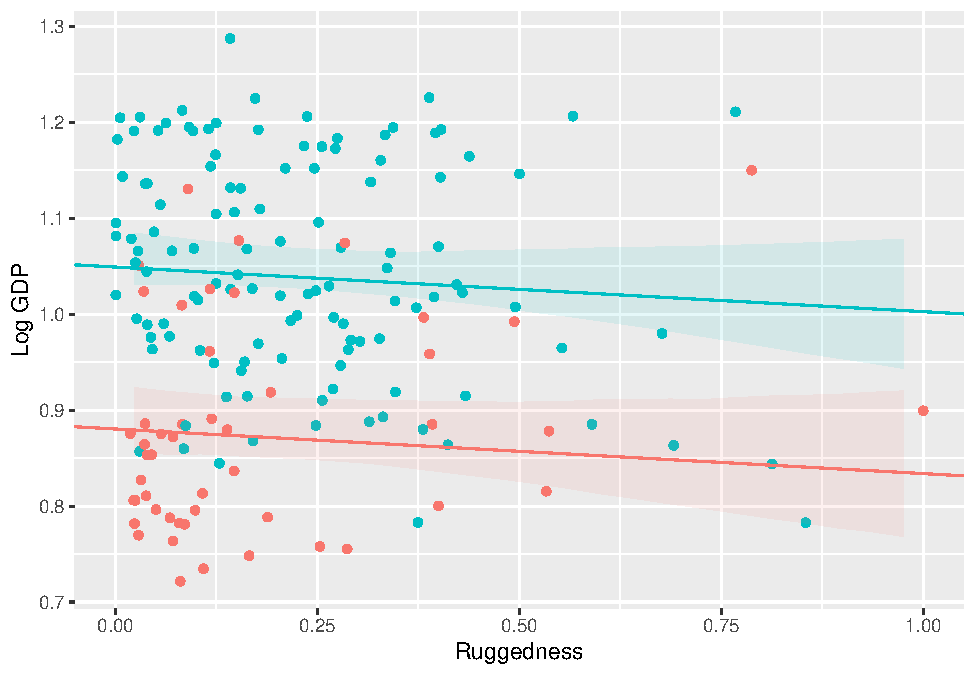
\includegraphics{02-small_worlds_files/figure-latex/unnamed-chunk-2-2.pdf} 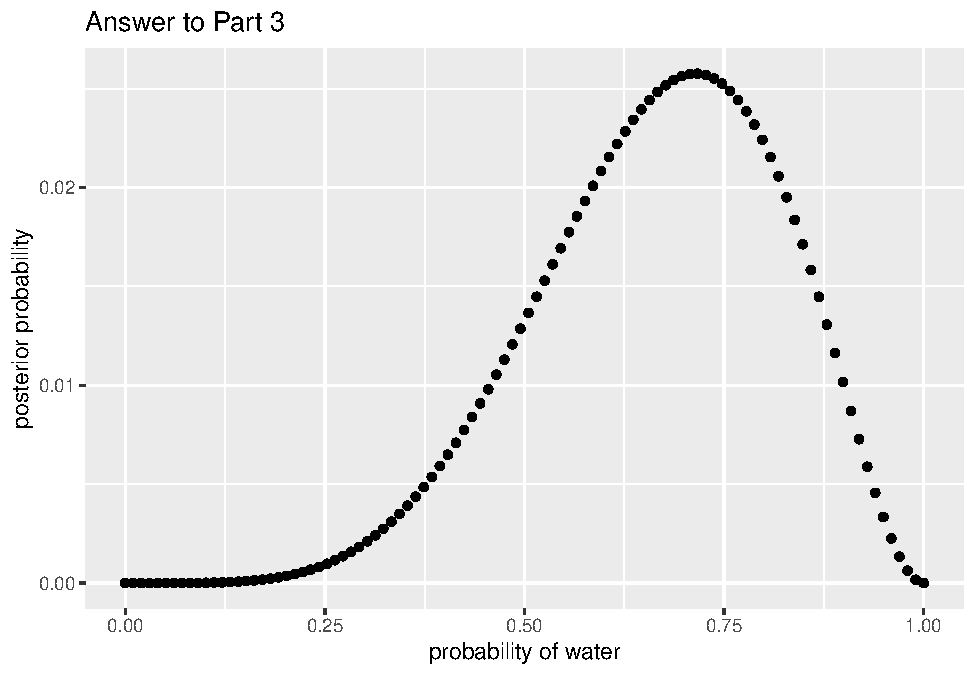
\includegraphics{02-small_worlds_files/figure-latex/unnamed-chunk-2-3.pdf}

\hypertarget{m2}{%
\subsection*{2M2}\label{m2}}
\addcontentsline{toc}{subsection}{2M2}

\hypertarget{question-5}{%
\subsubsection*{Question}\label{question-5}}
\addcontentsline{toc}{subsubsection}{Question}

\begin{quote}
Now assume a prior for p that is equal to zero when p \textless{} 0.5 and is a positive constant when p ≥ 0.5. Again compute and plot the grid approximate posterior distribution for each of the sets of observations in the problem just above.
\end{quote}

\hypertarget{answer-5}{%
\subsubsection*{Answer}\label{answer-5}}
\addcontentsline{toc}{subsubsection}{Answer}

\includegraphics{02-small_worlds_files/figure-latex/unnamed-chunk-3-1.pdf} 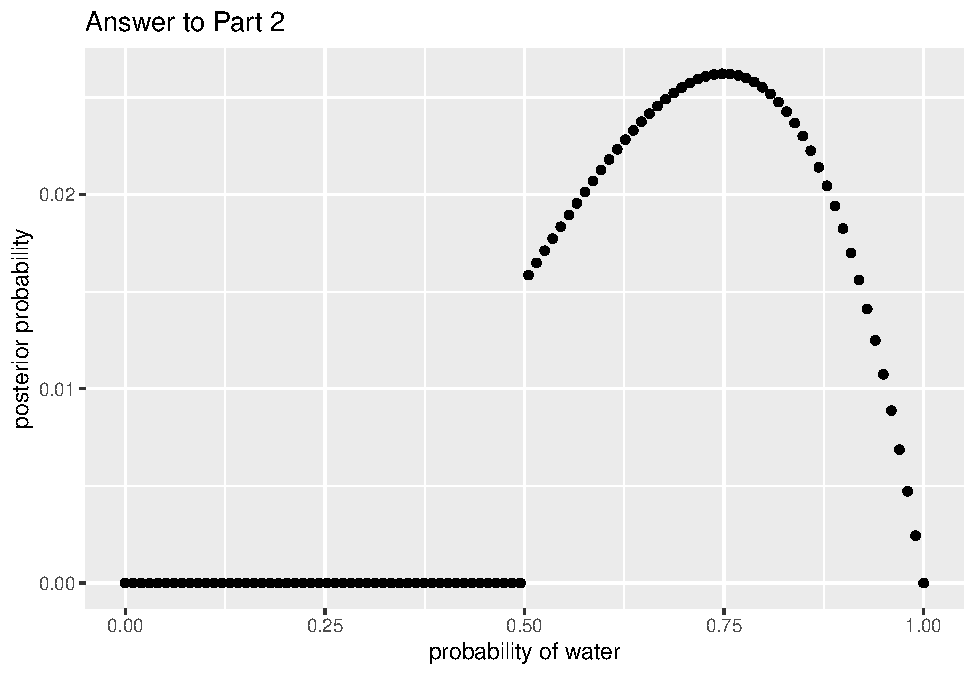
\includegraphics{02-small_worlds_files/figure-latex/unnamed-chunk-3-2.pdf} 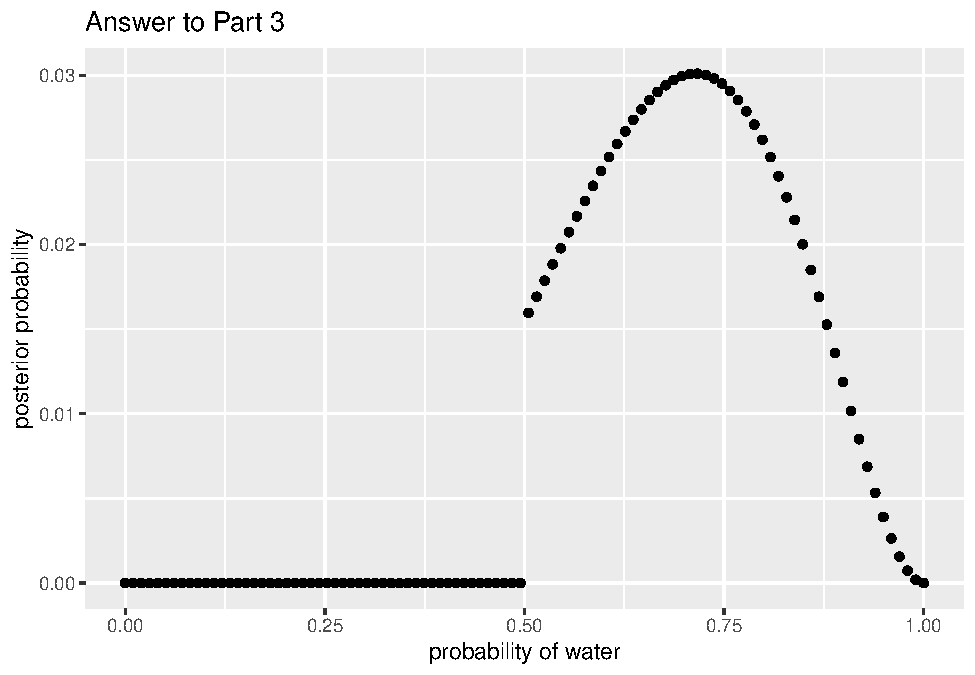
\includegraphics{02-small_worlds_files/figure-latex/unnamed-chunk-3-3.pdf}

\hypertarget{m3}{%
\subsection*{2M3}\label{m3}}
\addcontentsline{toc}{subsection}{2M3}

\hypertarget{question-6}{%
\subsubsection*{Question}\label{question-6}}
\addcontentsline{toc}{subsubsection}{Question}

\begin{quote}
Suppose there are two globes, one for Earth and one for Mars. The Earth globe is 70\% covered in water. The Mars globe is 100\% land. Further suppose that one of these globes --- you don't know which --- was tossed in the air and produced a ``land'' observation. Assume that each globe was equally likely to be tossed.

Show that the posterior probability that the globe was the Earth, conditional on seeing ``land'', \(\text{Pr}(Earth | Land)\), is 0.23.
\end{quote}

\hypertarget{answer-6}{%
\subsubsection*{Answer}\label{answer-6}}
\addcontentsline{toc}{subsubsection}{Answer}

Using Bayes Theorem:

\[
\text{Posterior} = \frac{\text{ prior * probability of the data }}{\text{ average probability of the data }}
\]

The numerator for our calculation will be the prior probability that the globe tossed was the Earth, multiplied by the likelihood of seeing land, assuming the globe tossed was the Earth: \(0.5 * 0.3\).

The denominator is the sum of these probabilities over each value of the prior. In this case, the prior probability of Mars * probability of seeing land given Mars + prior probability of the Earth * probability of seeing land given Earth: 0.5 * 1 + 0.5 * 0.3.

So we have \(\frac{ 0.5 * 0.3 } { 0.5 * 1 + 0.5 * 0.3 }\) which is

\begin{verbatim}
## [1] 0.2307692
\end{verbatim}

as required.

\hypertarget{m4}{%
\subsection*{2M4}\label{m4}}
\addcontentsline{toc}{subsection}{2M4}

\hypertarget{question-7}{%
\subsubsection*{Question}\label{question-7}}
\addcontentsline{toc}{subsubsection}{Question}

\begin{quote}
Suppose you have a deck with only three cards. Each card has two sides, and each side is either black or white. One card has two black sides. The second card has one black and one white side. The third card has two white sides. Now suppose all three cards are placed in a bag and shuffled. Someone reaches into the bag and pulls out a card and places it flat on a table. A black side is shown facing up, but you don't know the color of the side facing down.

Show that the probability that the other side is also black is 2/3. Use the counting method (Section 2 of the chapter) to approach this problem. This means counting up the ways that each card could produce the observed data (a black side facing up on the table).
\end{quote}

\hypertarget{answer-7}{%
\subsubsection*{Answer}\label{answer-7}}
\addcontentsline{toc}{subsubsection}{Answer}

We are looking for the posterior probability that we have chosen the black/black card (Card One), given that we see a black side facing up.

We assume for now that the chance of choosing each card is the same. That is that for every 1 way of choosing Card One, there is 1 way of choosing Card Two, and 1 way of choosing Card Three. Now we need to count up the number of ways of seeing a black side for each of the cards.

\begin{itemize}
\item
  Card One (black/black)
  There are two ways of seeing a black side after choosing this card - we could lay side one face up, or side two.
\item
  Card Two (black/white)
  There is only one way of seeing a black side after choosing this card - we would need to lay side one face up.
\item
  Card Three (white/white)
  There are no ways of seeing a black side after choosing this card.
\end{itemize}

Our calculation is \(\frac{1 * 2}{1 * 2 + 1 * 1 + 1 * 0} = \frac{2}{2+1+0} = \frac{2}{3}\).

\hypertarget{m5}{%
\subsection*{2M5}\label{m5}}
\addcontentsline{toc}{subsection}{2M5}

\hypertarget{question-8}{%
\subsubsection*{Question}\label{question-8}}
\addcontentsline{toc}{subsubsection}{Question}

\begin{quote}
Now suppose there are four cards: B/B, B/W, W/W, and another B/B. Again suppose a card is drawn from the bag and a black side appears face up. Again calculate the probability that the other side is black.
\end{quote}

\hypertarget{answer-8}{%
\subsubsection*{Answer}\label{answer-8}}
\addcontentsline{toc}{subsubsection}{Answer}

We are looking for the probability that we have chosen either Card One or Card Four.

Following the logic above, we get \(\frac{2 + 2}{2 + 2 + 1 + 0} = \frac{4}{5}\).

\hypertarget{m6}{%
\subsection*{2M6}\label{m6}}
\addcontentsline{toc}{subsection}{2M6}

\hypertarget{question-9}{%
\subsubsection*{Question}\label{question-9}}
\addcontentsline{toc}{subsubsection}{Question}

\begin{quote}
Imagine that black ink is heavy, and so cards with black sides are heavier than cards with white sides. As a result, it's less likely that a card with black sides is pulled from the bag. So again assume there are three cards: B/B, B/W, and W/W. After experimenting a number of times, you conclude that for every way to pull the B/B card from the bag, there are 2 ways to pull the B/W card and 3 ways to pull the W/W card. Again suppose that a card is pulled and a black side appears face up.

Show that the probability the other side is black is now 0.5. Use the counting method, as before.
\end{quote}

\hypertarget{answer-9}{%
\subsubsection*{Answer}\label{answer-9}}
\addcontentsline{toc}{subsubsection}{Answer}

We just replace the 1's from 2M4 with the new relative number of ways of pulling each card:

\begin{itemize}
\tightlist
\item
  B/B: 1 way
\item
  B/W: 2 ways
\item
  W/W: 3 ways
\end{itemize}

Our calculation is \(\frac{1 * 2}{1 * 2 + 2 * 1 + 3 * 0} = \frac{2}{2+2+0} = \frac{1}{2}\).

\hypertarget{m7}{%
\subsection*{2M7}\label{m7}}
\addcontentsline{toc}{subsection}{2M7}

\hypertarget{question-10}{%
\subsubsection*{Question}\label{question-10}}
\addcontentsline{toc}{subsubsection}{Question}

\begin{quote}
Assume again the original card problem, with a single card showing a black side face up. Before looking at the other side, we draw another card from the bag and lay it face up on the table. The face that is shown on the new card is white.

Show that the probability that the first card, the one showing a black side, has black on its other side is now 0.75. Use the counting method, if you can.

Hint: Treat this like the sequence of globe tosses, counting all the ways to see each observation, for each possible first card.
\end{quote}

\hypertarget{answer-10}{%
\subsubsection*{Answer}\label{answer-10}}
\addcontentsline{toc}{subsubsection}{Answer}

We are again looking for the probability that the first card we pulled was Card One (b/b), given the data (that we see one card with a black side and then one card with a white side).

we will use a table:

\begin{tabular}{l|r|r|r|r}
\hline
Cards & Prior Count & Black Side Count & White Side Count & Posterior Count\\
\hline
Card One & 1 & 2 & 3 & 6\\
\hline
Card Two & 1 & 1 & 2 & 2\\
\hline
Card Three & 1 & 0 & 1 & 0\\
\hline
\end{tabular}

For each row, we derive the White Side Counts by adding up the number of ways to see a white side for the two cards left in the bag. E.g. if we pulled Card One first, we have one card remaining with two white sides, and one card remaining with one white side = 3 white sides.

Our probability that we first pulled Card One is then \(\frac{6}{6+2} = 0.75\) as required.

\hypertarget{h1}{%
\subsection*{2H1}\label{h1}}
\addcontentsline{toc}{subsection}{2H1}

\hypertarget{question-11}{%
\subsubsection*{Question}\label{question-11}}
\addcontentsline{toc}{subsubsection}{Question}

\begin{quote}
Suppose there are two species of panda bear. Both are equally common in the wild and live in the same places. They look exactly alike and eat the same food, and there is yet no genetic assay capable of telling them apart. They differ however in their family sizes. Species A gives birth to twins 10\% of the time, otherwise birthing a single infant. Species B births twins 20\% of the time, otherwise birthing singleton infants. Assume these numbers are known with certainty, from many years of field research.

Now suppose you are managing a captive panda breeding program. You have a new female panda of unknown species, and she has just given birth to twins. What is the probability that her next birth will also be twins?
\end{quote}

\hypertarget{answer-11}{%
\subsubsection*{Answer}\label{answer-11}}
\addcontentsline{toc}{subsubsection}{Answer}

\begin{tabular}{l|r|r|r|r}
\hline
Species & Prior Count & Twins Count & Posterior Count & Posterior Probability\\
\hline
Species A & 1 & 1 & 1 & 0.33\\
\hline
Species B & 1 & 2 & 2 & 0.67\\
\hline
\end{tabular}

Probability of having twins is \(\text{probability of species } A * 0.1 + \text{probability of species } B * 0.2 = 1/3 * 0.1 + 2/3 * 0.2 = 1/6\).

\hypertarget{h2}{%
\subsection*{2H2}\label{h2}}
\addcontentsline{toc}{subsection}{2H2}

\hypertarget{question-12}{%
\subsubsection*{Question}\label{question-12}}
\addcontentsline{toc}{subsubsection}{Question}

\begin{quote}
Recall all the facts from the problem above. Now compute the probability that the panda we have is from species A, assuming we have observed only the first birth and that it was twins.
\end{quote}

\hypertarget{answer-12}{%
\subsubsection*{Answer}\label{answer-12}}
\addcontentsline{toc}{subsubsection}{Answer}

This questions implies that there was an easier way of answering the first question.

In any case, we have already calculated that the probability of species A is 1/3.

\hypertarget{h3}{%
\subsection*{2H3}\label{h3}}
\addcontentsline{toc}{subsection}{2H3}

\hypertarget{question-13}{%
\subsubsection*{Question}\label{question-13}}
\addcontentsline{toc}{subsubsection}{Question}

\begin{quote}
Continuing on from the previous problem, suppose the same panda mother has a second birth and that it is not twins, but a singleton infant. Compute the posterior probability that this panda is species A.
\end{quote}

\hypertarget{answer-13}{%
\subsubsection*{Answer}\label{answer-13}}
\addcontentsline{toc}{subsubsection}{Answer}

\begin{tabular}{l|r|r|r|r|r}
\hline
Species & Prior Count & Twins Count & Singleton Count & Posterior Count & Posterior Probability\\
\hline
Species A & 1 & 1 & 9 & 9 & 0.36\\
\hline
Species B & 1 & 2 & 8 & 16 & 0.64\\
\hline
\end{tabular}

The probability of species A is now 36\%.

\hypertarget{h4}{%
\subsection*{2H4}\label{h4}}
\addcontentsline{toc}{subsection}{2H4}

\hypertarget{question-14}{%
\subsubsection*{Question}\label{question-14}}
\addcontentsline{toc}{subsubsection}{Question}

\begin{quote}
A common boast of Bayesian statisticians is that Bayesian inference makes it easy to use all of the data, even if the data are of different types. So suppose now that a veterinarian comes along who has a new genetic test that she claims can identify the species of our mother panda. But the test, like all tests, is imperfect. This is the information you have about the test:

\begin{itemize}
\tightlist
\item
  The probability it correctly identifies a species A panda is 0.8.
\item
  The probability it correctly identifies a species B panda is 0.65.
\end{itemize}

The vet administers the test to your panda and tells you that the test is positive for species A. First ignore your previous information from the births and compute the posterior probability that your panda is species A. Then redo your calculation, now using the birth data as well.
\end{quote}

\hypertarget{answer-14}{%
\subsubsection*{Answer}\label{answer-14}}
\addcontentsline{toc}{subsubsection}{Answer}

Using test results alone:

\begin{tabular}{l|r|r|r|r}
\hline
Species & Prior Count & Test for A & Posterior Count & Posterior Probability\\
\hline
Species A & 1 & 8 & 8 & 0.8\\
\hline
Species B & 1 & 2 & 2 & 0.2\\
\hline
\end{tabular}

Using births and test results:

\begin{tabular}{l|r|r|r|r|r|r}
\hline
Species & Prior Count & Twins Count & Singleton Count & Test for A & Posterior Count & Posterior Probability\\
\hline
Species A & 1 & 1 & 9 & 8 & 72 & 0.69\\
\hline
Species B & 1 & 2 & 8 & 2 & 32 & 0.31\\
\hline
\end{tabular}

\hypertarget{further-reading-1}{%
\section*{Further Reading}\label{further-reading-1}}
\addcontentsline{toc}{section}{Further Reading}

\hypertarget{sampling_imaginary}{%
\chapter{Sampling the Imaginary}\label{sampling_imaginary}}

\hypertarget{chapter-notes-2}{%
\section{Chapter Notes}\label{chapter-notes-2}}

I haven't written chapter notes for the first five chapters.

\hypertarget{questions-2}{%
\section{Questions}\label{questions-2}}

\begin{quote}
The Easy problems use the samples from the posterior distribution for the globe tossing example. This code will give you a specific set of samples, so that you can check your answers exactly.
\end{quote}

\begin{Shaded}
\begin{Highlighting}[]
\NormalTok{p\_grid }\OtherTok{\textless{}{-}} \FunctionTok{seq}\NormalTok{( }\AttributeTok{from=}\DecValTok{0}\NormalTok{ , }\AttributeTok{to=}\DecValTok{1}\NormalTok{ , }\AttributeTok{length.out=}\DecValTok{1000}\NormalTok{ ) }

\NormalTok{prior }\OtherTok{\textless{}{-}} \FunctionTok{rep}\NormalTok{( }\DecValTok{1}\NormalTok{ , }\DecValTok{1000}\NormalTok{ ) }

\NormalTok{likelihood }\OtherTok{\textless{}{-}} \FunctionTok{dbinom}\NormalTok{( }\DecValTok{6}\NormalTok{ , }\AttributeTok{size=}\DecValTok{9}\NormalTok{ , }\AttributeTok{prob=}\NormalTok{p\_grid ) }

\NormalTok{posterior }\OtherTok{\textless{}{-}}\NormalTok{ likelihood }\SpecialCharTok{*}\NormalTok{ prior}

\NormalTok{posterior }\OtherTok{\textless{}{-}}\NormalTok{ posterior }\SpecialCharTok{/} \FunctionTok{sum}\NormalTok{(posterior)}

\FunctionTok{set.seed}\NormalTok{(}\DecValTok{100}\NormalTok{) }

\NormalTok{samples }\OtherTok{\textless{}{-}} \FunctionTok{sample}\NormalTok{( p\_grid , }\AttributeTok{prob=}\NormalTok{posterior , }\AttributeTok{size=}\FloatTok{1e4}\NormalTok{ , }\AttributeTok{replace=}\ConstantTok{TRUE}\NormalTok{ )}
\end{Highlighting}
\end{Shaded}

\hypertarget{e1-1}{%
\subsection*{3E1}\label{e1-1}}
\addcontentsline{toc}{subsection}{3E1}

\hypertarget{question-15}{%
\subsubsection*{Question}\label{question-15}}
\addcontentsline{toc}{subsubsection}{Question}

\begin{quote}
How much posterior probability lies below p = 0.2?
\end{quote}

\hypertarget{answer-15}{%
\subsubsection*{Answer}\label{answer-15}}
\addcontentsline{toc}{subsubsection}{Answer}

Here's the code:

\begin{Shaded}
\begin{Highlighting}[]
\CommentTok{\#Exact answer}
\FunctionTok{sum}\NormalTok{(posterior[p\_grid}\SpecialCharTok{\textless{}}\FloatTok{0.2}\NormalTok{])}\SpecialCharTok{*}\DecValTok{100}

\CommentTok{\#Sample answer}
\FunctionTok{sum}\NormalTok{(samples}\SpecialCharTok{\textless{}}\FloatTok{0.2}\NormalTok{)}\SpecialCharTok{/}\FunctionTok{length}\NormalTok{(samples)}\SpecialCharTok{*}\DecValTok{100}
\end{Highlighting}
\end{Shaded}

The exact answer is 0.09\% Sampling from the posterior suggests 0.04\%.

\hypertarget{e2-1}{%
\subsection*{3E2}\label{e2-1}}
\addcontentsline{toc}{subsection}{3E2}

\hypertarget{question-16}{%
\subsubsection*{Question}\label{question-16}}
\addcontentsline{toc}{subsubsection}{Question}

\begin{quote}
How much posterior probability lies above p = 0.8?
\end{quote}

\hypertarget{answer-16}{%
\subsubsection*{Answer}\label{answer-16}}
\addcontentsline{toc}{subsubsection}{Answer}

Similarly:

\begin{Shaded}
\begin{Highlighting}[]
\CommentTok{\#Exact answer}
\FunctionTok{sum}\NormalTok{(posterior[p\_grid}\SpecialCharTok{\textgreater{}}\FloatTok{0.8}\NormalTok{])}\SpecialCharTok{*}\DecValTok{100}

\CommentTok{\#Sample answer}
\FunctionTok{sum}\NormalTok{(samples}\SpecialCharTok{\textgreater{}}\FloatTok{0.8}\NormalTok{)}\SpecialCharTok{/}\FunctionTok{length}\NormalTok{(samples)}\SpecialCharTok{*}\DecValTok{100}
\end{Highlighting}
\end{Shaded}

The exact answer is 12.03\%. Sampling from the posterior suggests 11.16\%.

\hypertarget{e3-1}{%
\subsection*{3E3}\label{e3-1}}
\addcontentsline{toc}{subsection}{3E3}

\hypertarget{question-17}{%
\subsubsection*{Question}\label{question-17}}
\addcontentsline{toc}{subsubsection}{Question}

\begin{quote}
How much posterior probability lies between p = 0.2 and p = 0.8?
\end{quote}

\hypertarget{answer-17}{%
\subsubsection*{Answer}\label{answer-17}}
\addcontentsline{toc}{subsubsection}{Answer}

Code:

\begin{Shaded}
\begin{Highlighting}[]
\CommentTok{\#Exact answer}
\FunctionTok{sum}\NormalTok{(posterior[p\_grid }\SpecialCharTok{\textgreater{}} \FloatTok{0.2} \SpecialCharTok{\&}\NormalTok{ p\_grid }\SpecialCharTok{\textless{}} \FloatTok{0.8}\NormalTok{])}\SpecialCharTok{*}\DecValTok{100}

\CommentTok{\#Sample answer}
\FunctionTok{sum}\NormalTok{(samples }\SpecialCharTok{\textgreater{}} \FloatTok{0.2} \SpecialCharTok{\&}\NormalTok{ samples }\SpecialCharTok{\textless{}} \FloatTok{0.8}\NormalTok{)}\SpecialCharTok{/}\FunctionTok{length}\NormalTok{(samples)}\SpecialCharTok{*}\DecValTok{100}
\end{Highlighting}
\end{Shaded}

The exact answer is 87.88\%. Sampling from the posterior suggests 88.8\%.

\hypertarget{e4-1}{%
\subsection*{3E4}\label{e4-1}}
\addcontentsline{toc}{subsection}{3E4}

\hypertarget{question-18}{%
\subsubsection*{Question}\label{question-18}}
\addcontentsline{toc}{subsubsection}{Question}

\begin{quote}
20\% of the posterior probability lies below which value of p?
\end{quote}

\hypertarget{answer-18}{%
\subsubsection*{Answer}\label{answer-18}}
\addcontentsline{toc}{subsubsection}{Answer}

Code:

\begin{Shaded}
\begin{Highlighting}[]
\CommentTok{\#Exact answer}
\NormalTok{p\_grid[[}
  \FunctionTok{which}\NormalTok{(}\FunctionTok{cumsum}\NormalTok{(posterior)}\SpecialCharTok{\textgreater{}}\FloatTok{0.2}\NormalTok{)[[}\DecValTok{1}\NormalTok{]]}
\NormalTok{  ]]}

\CommentTok{\#Sample answer}
\FunctionTok{quantile}\NormalTok{(samples,}\FloatTok{0.2}\NormalTok{)}
\end{Highlighting}
\end{Shaded}

The exact answer suggests that 20\% of the posterior probability lies below p = 0.52. The sample answer suggests p = 0.52.

\hypertarget{e5}{%
\subsection*{3E5}\label{e5}}
\addcontentsline{toc}{subsection}{3E5}

\hypertarget{question-19}{%
\subsubsection*{Question}\label{question-19}}
\addcontentsline{toc}{subsubsection}{Question}

\begin{quote}
20\% of the posterior probability lies above which value of p?
\end{quote}

\hypertarget{answer-19}{%
\subsubsection*{Answer}\label{answer-19}}
\addcontentsline{toc}{subsubsection}{Answer}

Code:

\begin{Shaded}
\begin{Highlighting}[]
\CommentTok{\#Exact answer}
\NormalTok{p\_grid[[}
  \FunctionTok{which}\NormalTok{(}\FunctionTok{cumsum}\NormalTok{(posterior)}\SpecialCharTok{\textgreater{}}\FloatTok{0.8}\NormalTok{)[[}\DecValTok{1}\NormalTok{]]}
\NormalTok{  ]]}

\CommentTok{\#Sample answer}
\FunctionTok{quantile}\NormalTok{(samples,}\FloatTok{0.8}\NormalTok{)}
\end{Highlighting}
\end{Shaded}

The code checks the value of p such that 80\% of the posterior probability lies below p.~This is equivalent to 20\% lying above p.

The exact answer suggests p = 0.76. The sample answer suggests p = 0.76.

\hypertarget{e6}{%
\subsection*{3E6}\label{e6}}
\addcontentsline{toc}{subsection}{3E6}

\hypertarget{question-20}{%
\subsubsection*{Question}\label{question-20}}
\addcontentsline{toc}{subsubsection}{Question}

\begin{quote}
Which values of p contain the narrowest interval equal to 66\% of the posterior probability?
\end{quote}

\hypertarget{answer-20}{%
\subsubsection*{Answer}\label{answer-20}}
\addcontentsline{toc}{subsubsection}{Answer}

\begin{Shaded}
\begin{Highlighting}[]
\CommentTok{\#Sample answer}
\NormalTok{rethinking}\SpecialCharTok{::}\FunctionTok{HPDI}\NormalTok{(samples,}\AttributeTok{prob=}\FloatTok{0.66}\NormalTok{)}
\end{Highlighting}
\end{Shaded}

The interval (0.51 , 0.77) for p is the narrowest interval that contains 66\% of the posterior probability.

\hypertarget{e7}{%
\subsection*{3E7}\label{e7}}
\addcontentsline{toc}{subsection}{3E7}

\hypertarget{question-21}{%
\subsubsection*{Question}\label{question-21}}
\addcontentsline{toc}{subsubsection}{Question}

\begin{quote}
Which values of p contain 66\% of the posterior probability, assuming equal posterior probability both below and above the interval?
\end{quote}

\hypertarget{answer-21}{%
\subsubsection*{Answer}\label{answer-21}}
\addcontentsline{toc}{subsubsection}{Answer}

\begin{Shaded}
\begin{Highlighting}[]
\CommentTok{\#Sample answer}
\FunctionTok{quantile}\NormalTok{(samples,}\FunctionTok{c}\NormalTok{(}\FloatTok{0.17}\NormalTok{,}\FloatTok{0.83}\NormalTok{))}

\CommentTok{\#Figures calculated by splitting the remaining probability 0.34 in half above and below the desired interval.}
\CommentTok{\#quantile(samples,c( (1{-}0.66) / 2 ,1 {-} (1{-}0.66) / 2))}

\CommentTok{\#alternatively:}
\CommentTok{\#rethinking::PI(samples,0.66)}
\end{Highlighting}
\end{Shaded}

The interval (0.5 , 0.77) for p is the interval that contains 66\% of the posterior probability, assuming equal posterior probability both below and above the interval.

\hypertarget{m1-1}{%
\subsection*{3M1}\label{m1-1}}
\addcontentsline{toc}{subsection}{3M1}

\hypertarget{question-22}{%
\subsubsection*{Question}\label{question-22}}
\addcontentsline{toc}{subsubsection}{Question}

\begin{quote}
Suppose the globe tossing data had turned out to be 8 water in 15 tosses. Construct the posterior distribution, using grid approximation. Use the same flat prior as before.
\end{quote}

\hypertarget{answer-22}{%
\subsubsection*{Answer}\label{answer-22}}
\addcontentsline{toc}{subsubsection}{Answer}

\begin{Shaded}
\begin{Highlighting}[]
\NormalTok{p\_grid }\OtherTok{\textless{}{-}} \FunctionTok{seq}\NormalTok{(}\DecValTok{0}\NormalTok{,}\DecValTok{1}\NormalTok{,}\AttributeTok{length.out =} \FloatTok{1e4}\NormalTok{)}

\NormalTok{prior }\OtherTok{\textless{}{-}} \FunctionTok{rep}\NormalTok{(}\DecValTok{1}\NormalTok{,}\FloatTok{1e4}\NormalTok{)}

\CommentTok{\# This next line contains the only code change}
\NormalTok{likelihood }\OtherTok{\textless{}{-}} \FunctionTok{dbinom}\NormalTok{(}\DecValTok{8}\NormalTok{,}\AttributeTok{size=}\DecValTok{15}\NormalTok{,}\AttributeTok{prob=}\NormalTok{p\_grid)}

\NormalTok{posterior }\OtherTok{\textless{}{-}}\NormalTok{ prior }\SpecialCharTok{*}\NormalTok{ likelihood}

\NormalTok{posterior }\OtherTok{\textless{}{-}}\NormalTok{ posterior}\SpecialCharTok{/}\FunctionTok{sum}\NormalTok{(posterior)}
\end{Highlighting}
\end{Shaded}

\hypertarget{m2-1}{%
\subsection*{3M2}\label{m2-1}}
\addcontentsline{toc}{subsection}{3M2}

\hypertarget{question-23}{%
\subsubsection*{Question}\label{question-23}}
\addcontentsline{toc}{subsubsection}{Question}

\begin{quote}
Draw 10,000 samples from the grid approximation from above. Then use the samples to calculate the 90\% HPDI for p.
\end{quote}

\hypertarget{answer-23}{%
\subsubsection*{Answer}\label{answer-23}}
\addcontentsline{toc}{subsubsection}{Answer}

\begin{Shaded}
\begin{Highlighting}[]
\FunctionTok{set.seed}\NormalTok{(}\DecValTok{100}\NormalTok{) }

\NormalTok{samples }\OtherTok{\textless{}{-}} \FunctionTok{sample}\NormalTok{(p\_grid, }\AttributeTok{size=}\FloatTok{1e4}\NormalTok{, }\AttributeTok{prob=}\NormalTok{ posterior, }\AttributeTok{replace=}\ConstantTok{TRUE}\NormalTok{)}

\NormalTok{rethinking}\SpecialCharTok{::}\FunctionTok{HPDI}\NormalTok{(samples,}\FloatTok{0.9}\NormalTok{)}
\end{Highlighting}
\end{Shaded}

\begin{verbatim}
##      |0.9      0.9| 
## 0.3379338 0.7208721
\end{verbatim}

The interval (0.34 , 0.72) for p is the narrowest interval that contains 90\% of the posterior probability.

\hypertarget{m3-1}{%
\subsection*{3M3}\label{m3-1}}
\addcontentsline{toc}{subsection}{3M3}

\hypertarget{question-24}{%
\subsubsection*{Question}\label{question-24}}
\addcontentsline{toc}{subsubsection}{Question}

\begin{quote}
Construct a posterior predictive check for this model and data. This means simulate the distribution of samples, averaging over the posterior uncertainty in p.~What is the probability of observing 8 water in 15 tosses?
\end{quote}

\hypertarget{answer-24}{%
\subsubsection*{Answer}\label{answer-24}}
\addcontentsline{toc}{subsubsection}{Answer}

\begin{Shaded}
\begin{Highlighting}[]
\FunctionTok{set.seed}\NormalTok{(}\DecValTok{100}\NormalTok{) }

\NormalTok{post\_pred }\OtherTok{\textless{}{-}} \FunctionTok{rbinom}\NormalTok{(}\FloatTok{1e4}\NormalTok{, }\AttributeTok{size=}\DecValTok{15}\NormalTok{, }\AttributeTok{prob=}\NormalTok{samples)}

\FunctionTok{sum}\NormalTok{(post\_pred}\SpecialCharTok{==}\DecValTok{8}\NormalTok{)}\SpecialCharTok{/}\FunctionTok{length}\NormalTok{(post\_pred)}
\end{Highlighting}
\end{Shaded}

\begin{verbatim}
## [1] 0.1473
\end{verbatim}

There is a 14.7\% chance of observing 8 water in 15 tosses.

\hypertarget{m4-1}{%
\subsection*{3M4}\label{m4-1}}
\addcontentsline{toc}{subsection}{3M4}

\hypertarget{question-25}{%
\subsubsection*{Question}\label{question-25}}
\addcontentsline{toc}{subsubsection}{Question}

\begin{quote}
Using the posterior distribution constructed from the new (8/15) data, now calculate the probability of observing 6 water in 9 tosses.
\end{quote}

\hypertarget{answer-25}{%
\subsubsection*{Answer}\label{answer-25}}
\addcontentsline{toc}{subsubsection}{Answer}

\begin{Shaded}
\begin{Highlighting}[]
\FunctionTok{set.seed}\NormalTok{(}\DecValTok{100}\NormalTok{)}

\NormalTok{post\_pred }\OtherTok{\textless{}{-}} \FunctionTok{rbinom}\NormalTok{(}\FloatTok{1e4}\NormalTok{, }\AttributeTok{size=}\DecValTok{9}\NormalTok{, }\AttributeTok{prob=}\NormalTok{samples)}

\FunctionTok{sum}\NormalTok{(post\_pred}\SpecialCharTok{==}\DecValTok{6}\NormalTok{)}\SpecialCharTok{/}\FunctionTok{length}\NormalTok{(post\_pred)}
\end{Highlighting}
\end{Shaded}

\begin{verbatim}
## [1] 0.1804
\end{verbatim}

There is a 18.0\% chance of observing 6 water in 9 tosses.

\hypertarget{m5-1}{%
\subsection*{3M5}\label{m5-1}}
\addcontentsline{toc}{subsection}{3M5}

\hypertarget{question-26}{%
\subsubsection*{Question}\label{question-26}}
\addcontentsline{toc}{subsubsection}{Question}

\begin{quote}
Start over at 3M1, but now use a prior that is zero below p = 0.5 and a constant above p = 0.5. This corresponds to prior information that a majority of the Earth's surface is water. Repeat each problem above and compare the inferences. What difference does the better prior make? If it helps, compare inferences (using both priors) to the true value p = 0.7.
\end{quote}

\hypertarget{answer-26}{%
\subsubsection*{Answer}\label{answer-26}}
\addcontentsline{toc}{subsubsection}{Answer}

\begin{Shaded}
\begin{Highlighting}[]
\CommentTok{\#Recalculate the posterior distribution using the new prior}

\NormalTok{p\_grid }\OtherTok{\textless{}{-}} \FunctionTok{seq}\NormalTok{(}\DecValTok{0}\NormalTok{,}\DecValTok{1}\NormalTok{,}\AttributeTok{length.out =} \FloatTok{1e4}\NormalTok{)}

\NormalTok{new\_prior }\OtherTok{\textless{}{-}} \FunctionTok{c}\NormalTok{(}\FunctionTok{rep}\NormalTok{(}\DecValTok{0}\NormalTok{,}\FunctionTok{sum}\NormalTok{(p\_grid}\SpecialCharTok{\textless{}}\FloatTok{0.5}\NormalTok{)) , }\FunctionTok{rep}\NormalTok{(}\DecValTok{2}\NormalTok{,}\FunctionTok{length}\NormalTok{(p\_grid) }\SpecialCharTok{{-}} \FunctionTok{sum}\NormalTok{(p\_grid}\SpecialCharTok{\textless{}}\FloatTok{0.5}\NormalTok{)) )}

\NormalTok{likelihood }\OtherTok{\textless{}{-}} \FunctionTok{dbinom}\NormalTok{(}\DecValTok{8}\NormalTok{,}\AttributeTok{size=}\DecValTok{15}\NormalTok{,}\AttributeTok{prob=}\NormalTok{p\_grid)}

\NormalTok{new\_posterior }\OtherTok{\textless{}{-}}\NormalTok{ new\_prior }\SpecialCharTok{*}\NormalTok{ likelihood}

\NormalTok{new\_posterior }\OtherTok{\textless{}{-}}\NormalTok{ new\_posterior}\SpecialCharTok{/}\FunctionTok{sum}\NormalTok{(new\_posterior)}


\CommentTok{\#Draw 10,000 samples from the grid approximation. Then use the samples to calculate the 90\% HPDI for p.}

\FunctionTok{set.seed}\NormalTok{(}\DecValTok{100}\NormalTok{)}
\NormalTok{new\_samples }\OtherTok{\textless{}{-}} \FunctionTok{sample}\NormalTok{(p\_grid, }\AttributeTok{size=}\FloatTok{1e4}\NormalTok{, }\AttributeTok{prob=}\NormalTok{ new\_posterior, }\AttributeTok{replace=}\ConstantTok{TRUE}\NormalTok{)}

\NormalTok{rethinking}\SpecialCharTok{::}\FunctionTok{HPDI}\NormalTok{(new\_samples,}\FloatTok{0.9}\NormalTok{)}
\end{Highlighting}
\end{Shaded}

\begin{verbatim}
##      |0.9      0.9| 
## 0.5000500 0.7152715
\end{verbatim}

The 90\% highest probability density interval for p was previously (0.34 , 0.72), now it is (0.5 , 0.72). The HDPI is narrower directly as a consequence of the prior eliminating estimates of p below 0.5.

\begin{Shaded}
\begin{Highlighting}[]
\CommentTok{\#Construct a posterior predictive check for this model and data. This means simulate the distribution of samples, averaging over the posterior uncertainty in p. What is the probability of observing 8 water in 15 tosses?}

\FunctionTok{set.seed}\NormalTok{(}\DecValTok{100}\NormalTok{)}
\NormalTok{new\_post\_pred }\OtherTok{\textless{}{-}} \FunctionTok{rbinom}\NormalTok{(}\FloatTok{1e4}\NormalTok{, }\AttributeTok{size=}\DecValTok{15}\NormalTok{, }\AttributeTok{prob=}\NormalTok{new\_samples)}

\FunctionTok{sum}\NormalTok{(new\_post\_pred}\SpecialCharTok{==}\DecValTok{8}\NormalTok{)}\SpecialCharTok{/}\FunctionTok{length}\NormalTok{(new\_post\_pred)}
\end{Highlighting}
\end{Shaded}

\begin{verbatim}
## [1] 0.1567
\end{verbatim}

\begin{Shaded}
\begin{Highlighting}[]
\CommentTok{\#true probability of seeing water 8 times in 15 tosses}
\FunctionTok{dbinom}\NormalTok{(}\DecValTok{8}\NormalTok{,}\DecValTok{15}\NormalTok{,}\AttributeTok{prob=}\FloatTok{0.7}\NormalTok{)}
\end{Highlighting}
\end{Shaded}

\begin{verbatim}
## [1] 0.08113003
\end{verbatim}

There was previously a 14.7\% chance of observing 8 water in 15 tosses. Now that probability is 15.7\%. The model is trained on data of 8 water observations in 15 tosses, and the probability of reproducing that data from the posterior doesn't seem to change much with our new prior. The true probability is much lower, around 8\% (setting p=70\%).

\begin{Shaded}
\begin{Highlighting}[]
\CommentTok{\#Using the posterior distribution constructed from the new (8/15) data, now calculate the probability of observing 6 water in 9 tosses.}

\FunctionTok{set.seed}\NormalTok{(}\DecValTok{100}\NormalTok{)}
\NormalTok{new\_post\_pred }\OtherTok{\textless{}{-}} \FunctionTok{rbinom}\NormalTok{(}\FloatTok{1e4}\NormalTok{, }\AttributeTok{size=}\DecValTok{9}\NormalTok{, }\AttributeTok{prob=}\NormalTok{new\_samples)}

\FunctionTok{sum}\NormalTok{(new\_post\_pred}\SpecialCharTok{==}\DecValTok{6}\NormalTok{)}\SpecialCharTok{/}\FunctionTok{length}\NormalTok{(new\_post\_pred)}
\end{Highlighting}
\end{Shaded}

\begin{verbatim}
## [1] 0.2292
\end{verbatim}

\begin{Shaded}
\begin{Highlighting}[]
\CommentTok{\#true probability of seeing water 6 times in 9 tosses}
\FunctionTok{dbinom}\NormalTok{(}\DecValTok{6}\NormalTok{,}\DecValTok{9}\NormalTok{,}\AttributeTok{prob=}\FloatTok{0.7}\NormalTok{)}
\end{Highlighting}
\end{Shaded}

\begin{verbatim}
## [1] 0.2668279
\end{verbatim}

There was previously a 18.0\% chance of observing 6 water in 9 tosses. Now that probability is 22.9\%. The model with the new prior does a slightly better job of approximating the true probability of 26.7\%

\hypertarget{m6-1}{%
\subsection*{3M6}\label{m6-1}}
\addcontentsline{toc}{subsection}{3M6}

\hypertarget{question-27}{%
\subsubsection*{Question}\label{question-27}}
\addcontentsline{toc}{subsubsection}{Question}

\begin{quote}
Suppose you want to estimate the Earth's proportion of water very precisely. Specifically, you want the 99\% percentile interval of the posterior distribution of p to be only 0.05 wide. This means the distance between the upper and lower bound of the interval should be 0.05. How many times will you have to toss the globe to do this?
\end{quote}

\hypertarget{answer-27}{%
\subsubsection*{Answer}\label{answer-27}}
\addcontentsline{toc}{subsubsection}{Answer}

I found this one to be quite tricky.

I ended up just looping through sample sizes from 1 to 10000 and measuring the width of the 99\% confidence interval for each size.

One thing that's unsatisfying about this approach is that I've had to assume a number of ``successes'' for each i number of trials. I've assumed that successes occur roughly in the 8 out of 15 proportion seen in the chapter example, but should it be the case that the number of trials required to get a percentile interval to a target width should be dependent on the proportion of successes?

Also, you'd think there might be an analytical approach since we know the distribution is binomial, but I've just brute forced an answer using a loop.

\begin{Shaded}
\begin{Highlighting}[]
\NormalTok{p\_grid }\OtherTok{\textless{}{-}} \FunctionTok{seq}\NormalTok{( }\AttributeTok{from=}\DecValTok{0}\NormalTok{ , }\AttributeTok{to=}\DecValTok{1}\NormalTok{ , }\AttributeTok{length.out=}\DecValTok{1000}\NormalTok{ ) }

\NormalTok{prior }\OtherTok{\textless{}{-}} \FunctionTok{rep}\NormalTok{( }\DecValTok{1}\NormalTok{ , }\DecValTok{1000}\NormalTok{ ) }

\NormalTok{width }\OtherTok{\textless{}{-}} \FunctionTok{list}\NormalTok{()}

\ControlFlowTok{for}\NormalTok{ (i }\ControlFlowTok{in} \FunctionTok{seq}\NormalTok{(}\DecValTok{1}\NormalTok{,}\DecValTok{10000}\NormalTok{))\{}
  
\NormalTok{  likelihood }\OtherTok{\textless{}{-}} \FunctionTok{dbinom}\NormalTok{( }\FunctionTok{round}\NormalTok{(i}\SpecialCharTok{*}\DecValTok{8}\SpecialCharTok{/}\DecValTok{15}\NormalTok{,}\AttributeTok{digits =} \DecValTok{0}\NormalTok{) , }\AttributeTok{size=}\NormalTok{i , }\AttributeTok{prob=}\NormalTok{p\_grid ) }
  
\NormalTok{  posterior }\OtherTok{\textless{}{-}}\NormalTok{ likelihood }\SpecialCharTok{*}\NormalTok{ prior}
  
\NormalTok{  posterior }\OtherTok{\textless{}{-}}\NormalTok{ posterior }\SpecialCharTok{/} \FunctionTok{sum}\NormalTok{(posterior)}
  
  \FunctionTok{set.seed}\NormalTok{(}\DecValTok{100}\NormalTok{) }
  
\NormalTok{  samples }\OtherTok{\textless{}{-}} \FunctionTok{sample}\NormalTok{( p\_grid , }\AttributeTok{prob=}\NormalTok{posterior , }\AttributeTok{size=}\FloatTok{1e4}\NormalTok{ , }\AttributeTok{replace=}\ConstantTok{TRUE}\NormalTok{ )}
  
\NormalTok{  interval }\OtherTok{\textless{}{-}}\NormalTok{ rethinking}\SpecialCharTok{::}\FunctionTok{PI}\NormalTok{(samples,}\FloatTok{0.99}\NormalTok{)}

\NormalTok{  width[i] }\OtherTok{\textless{}{-}}\NormalTok{ interval[}\DecValTok{2}\NormalTok{]}\SpecialCharTok{{-}}\NormalTok{interval[}\DecValTok{1}\NormalTok{]}
  
\NormalTok{\}}

 \FunctionTok{which}\NormalTok{(width}\SpecialCharTok{\textless{}}\FloatTok{0.05}\NormalTok{)[}\DecValTok{1}\NormalTok{]}
\end{Highlighting}
\end{Shaded}

\begin{verbatim}
## [1] 2731
\end{verbatim}

This method suggests 2731 trials should be sufficient.

This is one to revisit in the future.

\hypertarget{h1-1}{%
\subsection*{3H1}\label{h1-1}}
\addcontentsline{toc}{subsection}{3H1}

\begin{quote}
The Hard problems here all use the data below. These data indicate the gender (male=1, female=0) of officially reported first and second born children in 100 two-child families.
\end{quote}

\begin{Shaded}
\begin{Highlighting}[]
\NormalTok{birth1 }\OtherTok{\textless{}{-}} \FunctionTok{c}\NormalTok{(}\DecValTok{1}\NormalTok{,}\DecValTok{0}\NormalTok{,}\DecValTok{0}\NormalTok{,}\DecValTok{0}\NormalTok{,}\DecValTok{1}\NormalTok{,}\DecValTok{1}\NormalTok{,}\DecValTok{0}\NormalTok{,}\DecValTok{1}\NormalTok{,}\DecValTok{0}\NormalTok{,}\DecValTok{1}\NormalTok{,}\DecValTok{0}\NormalTok{,}\DecValTok{0}\NormalTok{,}\DecValTok{1}\NormalTok{,}\DecValTok{1}\NormalTok{,}\DecValTok{0}\NormalTok{,}\DecValTok{1}\NormalTok{,}\DecValTok{1}\NormalTok{,}\DecValTok{0}\NormalTok{,}\DecValTok{0}\NormalTok{,}\DecValTok{0}\NormalTok{,}\DecValTok{1}\NormalTok{,}\DecValTok{0}\NormalTok{,}\DecValTok{0}\NormalTok{,}\DecValTok{0}\NormalTok{,}\DecValTok{1}\NormalTok{,}\DecValTok{0}\NormalTok{, }\DecValTok{0}\NormalTok{,}\DecValTok{0}\NormalTok{,}\DecValTok{0}\NormalTok{,}\DecValTok{1}\NormalTok{,}\DecValTok{1}\NormalTok{,}\DecValTok{1}\NormalTok{,}\DecValTok{0}\NormalTok{,}\DecValTok{1}\NormalTok{,}\DecValTok{0}\NormalTok{,}\DecValTok{1}\NormalTok{,}\DecValTok{1}\NormalTok{,}\DecValTok{1}\NormalTok{,}\DecValTok{0}\NormalTok{,}\DecValTok{1}\NormalTok{,}\DecValTok{0}\NormalTok{,}\DecValTok{1}\NormalTok{,}\DecValTok{1}\NormalTok{,}\DecValTok{0}\NormalTok{,}\DecValTok{1}\NormalTok{,}\DecValTok{0}\NormalTok{,}\DecValTok{0}\NormalTok{,}\DecValTok{1}\NormalTok{,}\DecValTok{1}\NormalTok{,}\DecValTok{0}\NormalTok{,}\DecValTok{1}\NormalTok{,}\DecValTok{0}\NormalTok{,}\DecValTok{0}\NormalTok{,}\DecValTok{0}\NormalTok{,}\DecValTok{0}\NormalTok{,}\DecValTok{0}\NormalTok{,}\DecValTok{0}\NormalTok{,}\DecValTok{0}\NormalTok{, }\DecValTok{1}\NormalTok{,}\DecValTok{1}\NormalTok{,}\DecValTok{0}\NormalTok{,}\DecValTok{1}\NormalTok{,}\DecValTok{0}\NormalTok{,}\DecValTok{0}\NormalTok{,}\DecValTok{1}\NormalTok{,}\DecValTok{0}\NormalTok{,}\DecValTok{0}\NormalTok{,}\DecValTok{0}\NormalTok{,}\DecValTok{1}\NormalTok{,}\DecValTok{0}\NormalTok{,}\DecValTok{0}\NormalTok{,}\DecValTok{1}\NormalTok{,}\DecValTok{1}\NormalTok{,}\DecValTok{1}\NormalTok{,}\DecValTok{1}\NormalTok{,}\DecValTok{0}\NormalTok{,}\DecValTok{1}\NormalTok{,}\DecValTok{0}\NormalTok{,}\DecValTok{1}\NormalTok{,}\DecValTok{1}\NormalTok{,}\DecValTok{1}\NormalTok{,}\DecValTok{1}\NormalTok{,}\DecValTok{1}\NormalTok{,}\DecValTok{0}\NormalTok{,}\DecValTok{0}\NormalTok{,}\DecValTok{1}\NormalTok{,}\DecValTok{0}\NormalTok{,}\DecValTok{1}\NormalTok{,}\DecValTok{1}\NormalTok{,}\DecValTok{0}\NormalTok{, }\DecValTok{1}\NormalTok{,}\DecValTok{0}\NormalTok{,}\DecValTok{1}\NormalTok{,}\DecValTok{1}\NormalTok{,}\DecValTok{1}\NormalTok{,}\DecValTok{0}\NormalTok{,}\DecValTok{1}\NormalTok{,}\DecValTok{1}\NormalTok{,}\DecValTok{1}\NormalTok{,}\DecValTok{1}\NormalTok{) }


\NormalTok{birth2 }\OtherTok{\textless{}{-}} \FunctionTok{c}\NormalTok{(}\DecValTok{0}\NormalTok{,}\DecValTok{1}\NormalTok{,}\DecValTok{0}\NormalTok{,}\DecValTok{1}\NormalTok{,}\DecValTok{0}\NormalTok{,}\DecValTok{1}\NormalTok{,}\DecValTok{1}\NormalTok{,}\DecValTok{1}\NormalTok{,}\DecValTok{0}\NormalTok{,}\DecValTok{0}\NormalTok{,}\DecValTok{1}\NormalTok{,}\DecValTok{1}\NormalTok{,}\DecValTok{1}\NormalTok{,}\DecValTok{1}\NormalTok{,}\DecValTok{1}\NormalTok{,}\DecValTok{0}\NormalTok{,}\DecValTok{0}\NormalTok{,}\DecValTok{1}\NormalTok{,}\DecValTok{1}\NormalTok{,}\DecValTok{1}\NormalTok{,}\DecValTok{0}\NormalTok{,}\DecValTok{0}\NormalTok{,}\DecValTok{1}\NormalTok{,}\DecValTok{1}\NormalTok{,}\DecValTok{1}\NormalTok{,}\DecValTok{0}\NormalTok{, }\DecValTok{1}\NormalTok{,}\DecValTok{1}\NormalTok{,}\DecValTok{1}\NormalTok{,}\DecValTok{0}\NormalTok{,}\DecValTok{1}\NormalTok{,}\DecValTok{1}\NormalTok{,}\DecValTok{1}\NormalTok{,}\DecValTok{0}\NormalTok{,}\DecValTok{1}\NormalTok{,}\DecValTok{0}\NormalTok{,}\DecValTok{0}\NormalTok{,}\DecValTok{1}\NormalTok{,}\DecValTok{1}\NormalTok{,}\DecValTok{1}\NormalTok{,}\DecValTok{1}\NormalTok{,}\DecValTok{0}\NormalTok{,}\DecValTok{0}\NormalTok{,}\DecValTok{1}\NormalTok{,}\DecValTok{0}\NormalTok{,}\DecValTok{1}\NormalTok{,}\DecValTok{1}\NormalTok{,}\DecValTok{1}\NormalTok{,}\DecValTok{1}\NormalTok{,}\DecValTok{1}\NormalTok{,}\DecValTok{1}\NormalTok{,}\DecValTok{1}\NormalTok{,}\DecValTok{1}\NormalTok{,}\DecValTok{1}\NormalTok{,}\DecValTok{1}\NormalTok{,}\DecValTok{1}\NormalTok{,}\DecValTok{1}\NormalTok{,}\DecValTok{1}\NormalTok{, }\DecValTok{1}\NormalTok{,}\DecValTok{1}\NormalTok{,}\DecValTok{1}\NormalTok{,}\DecValTok{0}\NormalTok{,}\DecValTok{1}\NormalTok{,}\DecValTok{1}\NormalTok{,}\DecValTok{0}\NormalTok{,}\DecValTok{1}\NormalTok{,}\DecValTok{1}\NormalTok{,}\DecValTok{0}\NormalTok{,}\DecValTok{1}\NormalTok{,}\DecValTok{1}\NormalTok{,}\DecValTok{1}\NormalTok{,}\DecValTok{0}\NormalTok{,}\DecValTok{0}\NormalTok{,}\DecValTok{0}\NormalTok{,}\DecValTok{0}\NormalTok{,}\DecValTok{0}\NormalTok{,}\DecValTok{0}\NormalTok{,}\DecValTok{1}\NormalTok{,}\DecValTok{0}\NormalTok{,}\DecValTok{0}\NormalTok{,}\DecValTok{0}\NormalTok{,}\DecValTok{1}\NormalTok{,}\DecValTok{1}\NormalTok{,}\DecValTok{0}\NormalTok{,}\DecValTok{0}\NormalTok{,}\DecValTok{1}\NormalTok{,}\DecValTok{0}\NormalTok{,}\DecValTok{0}\NormalTok{,}\DecValTok{1}\NormalTok{,}\DecValTok{1}\NormalTok{,}\DecValTok{0}\NormalTok{,}\DecValTok{0}\NormalTok{,}\DecValTok{0}\NormalTok{,}\DecValTok{1}\NormalTok{,}\DecValTok{1}\NormalTok{,}\DecValTok{1}\NormalTok{,}\DecValTok{0}\NormalTok{,}\DecValTok{0}\NormalTok{,}\DecValTok{0}\NormalTok{,}\DecValTok{0}\NormalTok{)}
\end{Highlighting}
\end{Shaded}

\begin{quote}
So for example, the first family in the data reported a boy (1) and then a girl (0). The second family reported a girl (0) and then a boy (1). The third family reported two girls.
\end{quote}

\hypertarget{question-28}{%
\subsubsection*{Question}\label{question-28}}
\addcontentsline{toc}{subsubsection}{Question}

\begin{quote}
Using grid approximation, compute the posterior distribution for the probability of a birth being a boy. Assume a uniform prior probability. Which parameter value maximizes the posterior probability?
\end{quote}

\hypertarget{answer-28}{%
\subsubsection*{Answer}\label{answer-28}}
\addcontentsline{toc}{subsubsection}{Answer}

We assume for the moment that gender is independent of birth order. Then we have a binomial distribution with an unknown parameter p, which is the target of our inference.

\begin{Shaded}
\begin{Highlighting}[]
\CommentTok{\#observations in our data {-} this will form our likelihood}

\NormalTok{births}\OtherTok{=}\FunctionTok{length}\NormalTok{(birth1)}\SpecialCharTok{+}\FunctionTok{length}\NormalTok{(birth2)}

\NormalTok{boys}\OtherTok{=}\FunctionTok{sum}\NormalTok{(birth1)}\SpecialCharTok{+}\FunctionTok{sum}\NormalTok{(birth2)}

\CommentTok{\#standard grid approximation approach seen above}

\NormalTok{p\_grid }\OtherTok{\textless{}{-}} \FunctionTok{seq}\NormalTok{( }\AttributeTok{from=}\DecValTok{0}\NormalTok{ , }\AttributeTok{to=}\DecValTok{1}\NormalTok{ , }\AttributeTok{length.out=}\DecValTok{1000}\NormalTok{ ) }

\NormalTok{prior }\OtherTok{\textless{}{-}} \FunctionTok{rep}\NormalTok{( }\DecValTok{1}\NormalTok{ , }\DecValTok{1000}\NormalTok{ ) }

\NormalTok{likelihood }\OtherTok{\textless{}{-}} \FunctionTok{dbinom}\NormalTok{(boys , }\AttributeTok{size=}\NormalTok{ births, }\AttributeTok{prob=}\NormalTok{p\_grid ) }
  
\NormalTok{posterior }\OtherTok{\textless{}{-}}\NormalTok{ likelihood }\SpecialCharTok{*}\NormalTok{ prior}
  
\NormalTok{posterior }\OtherTok{\textless{}{-}}\NormalTok{ posterior }\SpecialCharTok{/} \FunctionTok{sum}\NormalTok{(posterior)}


\CommentTok{\#Which parameter value maximizes the posterior probability?}

\CommentTok{\#We sample from the posterior as before, and find the mode.}
  
\FunctionTok{set.seed}\NormalTok{(}\DecValTok{100}\NormalTok{) }
  
\NormalTok{samples }\OtherTok{\textless{}{-}} \FunctionTok{sample}\NormalTok{( p\_grid , }\AttributeTok{prob=}\NormalTok{posterior , }\AttributeTok{size=}\FloatTok{1e4}\NormalTok{ , }\AttributeTok{replace=}\ConstantTok{TRUE}\NormalTok{ )}

\NormalTok{rethinking}\SpecialCharTok{::}\FunctionTok{chainmode}\NormalTok{(samples)}
\end{Highlighting}
\end{Shaded}

\begin{verbatim}
## [1] 0.5552446
\end{verbatim}

The parameter value that maximises the posterior probability is 55.5\%.

\hypertarget{h2-1}{%
\subsection*{3H2}\label{h2-1}}
\addcontentsline{toc}{subsection}{3H2}

\hypertarget{question-29}{%
\subsubsection*{Question}\label{question-29}}
\addcontentsline{toc}{subsubsection}{Question}

\begin{quote}
Using the sample function, draw 10,000 random parameter values from the posterior distribution you calculated above. Use these samples to estimate the 50\%, 89\%, and 97\% highest posterior density intervals.
\end{quote}

\hypertarget{answer-29}{%
\subsubsection*{Answer}\label{answer-29}}
\addcontentsline{toc}{subsubsection}{Answer}

I could have answered the last question analytically by using which.max(posterior)/1000, but since I used samples we're well set up for this question.

\begin{Shaded}
\begin{Highlighting}[]
\FunctionTok{set.seed}\NormalTok{(}\DecValTok{100}\NormalTok{)}

\NormalTok{rethinking}\SpecialCharTok{::}\FunctionTok{HPDI}\NormalTok{(samples, }\FloatTok{0.5}\NormalTok{)}
\end{Highlighting}
\end{Shaded}

\begin{verbatim}
##      |0.5      0.5| 
## 0.5265265 0.5725726
\end{verbatim}

\begin{Shaded}
\begin{Highlighting}[]
\NormalTok{rethinking}\SpecialCharTok{::}\FunctionTok{HPDI}\NormalTok{(samples, }\FloatTok{0.89}\NormalTok{)}
\end{Highlighting}
\end{Shaded}

\begin{verbatim}
##     |0.89     0.89| 
## 0.4994995 0.6076076
\end{verbatim}

\begin{Shaded}
\begin{Highlighting}[]
\NormalTok{rethinking}\SpecialCharTok{::}\FunctionTok{HPDI}\NormalTok{(samples, }\FloatTok{0.97}\NormalTok{)}
\end{Highlighting}
\end{Shaded}

\begin{verbatim}
##     |0.97     0.97| 
## 0.4824825 0.6296296
\end{verbatim}

The narrowest interval for p that contains 50\% of the posterior distribution is (0.527 , 0.573).

The narrowest interval for p that contains 89\% of the posterior distribution is (0.499 , 0.608).

The narrowest interval for p that contains 97\% of the posterior distribution is (0.482 , 0.630).

\hypertarget{h3-1}{%
\subsection*{3H3}\label{h3-1}}
\addcontentsline{toc}{subsection}{3H3}

\hypertarget{question-30}{%
\subsubsection*{Question}\label{question-30}}
\addcontentsline{toc}{subsubsection}{Question}

\begin{quote}
Use rbinom to simulate 10,000 replicates of 200 births. You should end up with 10,000 numbers, each one a count of boys out of 200 births. Compare the distribution of predicted numbers of boys to the actual count in the data (111 boys out of 200 births). There are many good ways to visualize the simulations, but the dens command (part of the rethinking package) is probably the easiest way in this case.

Does it look like the model fits the data well? That is, does the distribution of predictions include the actual observation as a central, likely outcome?
\end{quote}

\hypertarget{answer-30}{%
\subsubsection*{Answer}\label{answer-30}}
\addcontentsline{toc}{subsubsection}{Answer}

\begin{Shaded}
\begin{Highlighting}[]
\FunctionTok{set.seed}\NormalTok{(}\DecValTok{100}\NormalTok{)}

\NormalTok{post\_pred }\OtherTok{\textless{}{-}} \FunctionTok{rbinom}\NormalTok{(}\FloatTok{1e4}\NormalTok{,}\DecValTok{200}\NormalTok{, samples)}

\NormalTok{rethinking}\SpecialCharTok{::}\FunctionTok{simplehist}\NormalTok{(post\_pred)}
\end{Highlighting}
\end{Shaded}

\includegraphics{03-sampling_imaginary_files/figure-latex/unnamed-chunk-21-1.pdf}

\begin{Shaded}
\begin{Highlighting}[]
\NormalTok{rethinking}\SpecialCharTok{::}\FunctionTok{dens}\NormalTok{(post\_pred)}
\end{Highlighting}
\end{Shaded}

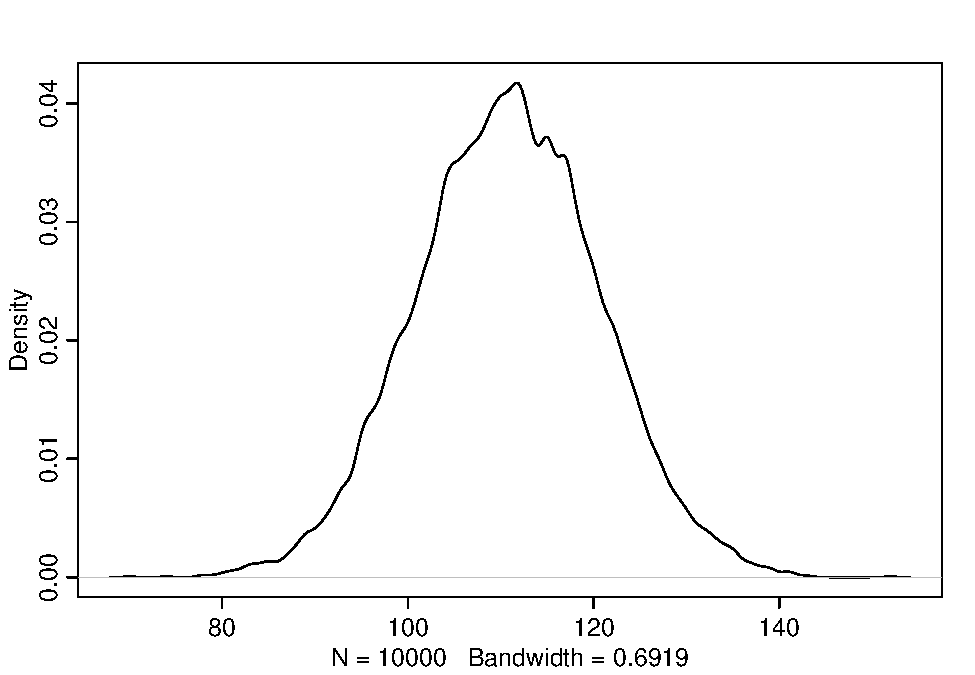
\includegraphics{03-sampling_imaginary_files/figure-latex/unnamed-chunk-21-2.pdf}

The model appears to fit the data well, at least in the sense described: that the distribution of predictions includes the actual observation as a central, likely outcome.

\hypertarget{h4-1}{%
\subsection*{3H4}\label{h4-1}}
\addcontentsline{toc}{subsection}{3H4}

\hypertarget{question-31}{%
\subsubsection*{Question}\label{question-31}}
\addcontentsline{toc}{subsubsection}{Question}

\begin{quote}
Now compare 10,000 counts of boys from 100 simulated first borns only to the number of boys in the first births, birth1. How does the model look in this light?
\end{quote}

\hypertarget{answer-31}{%
\subsubsection*{Answer}\label{answer-31}}
\addcontentsline{toc}{subsubsection}{Answer}

\begin{Shaded}
\begin{Highlighting}[]
\FunctionTok{sum}\NormalTok{(birth1)}
\end{Highlighting}
\end{Shaded}

\begin{verbatim}
## [1] 51
\end{verbatim}

\begin{Shaded}
\begin{Highlighting}[]
\FunctionTok{set.seed}\NormalTok{(}\DecValTok{100}\NormalTok{)}

\NormalTok{post\_pred }\OtherTok{\textless{}{-}} \FunctionTok{rbinom}\NormalTok{(}\FloatTok{1e4}\NormalTok{,}\DecValTok{100}\NormalTok{, samples)}

\NormalTok{rethinking}\SpecialCharTok{::}\FunctionTok{simplehist}\NormalTok{(post\_pred)}
\end{Highlighting}
\end{Shaded}

\includegraphics{03-sampling_imaginary_files/figure-latex/unnamed-chunk-22-1.pdf}

\begin{Shaded}
\begin{Highlighting}[]
\NormalTok{rethinking}\SpecialCharTok{::}\FunctionTok{dens}\NormalTok{(post\_pred)}
\end{Highlighting}
\end{Shaded}

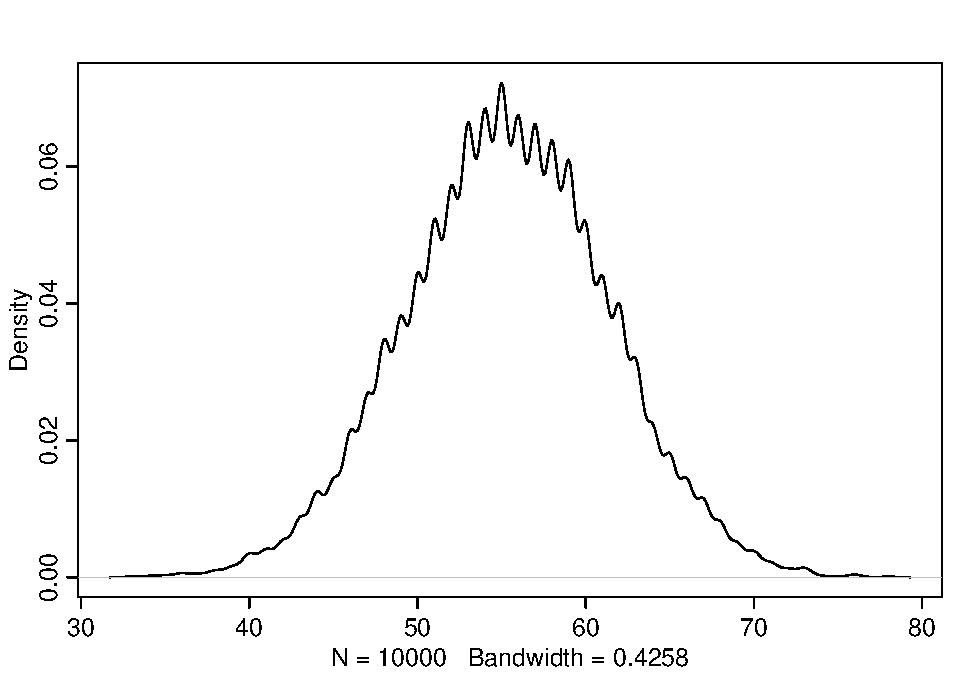
\includegraphics{03-sampling_imaginary_files/figure-latex/unnamed-chunk-22-2.pdf}

The model does a much worse job here. The true number of boys in birth1 is 51 out of 100, while the most likely outcomes expected by the model are closer to 55, 56.

\hypertarget{h5}{%
\subsection*{3H5}\label{h5}}
\addcontentsline{toc}{subsection}{3H5}

\hypertarget{question-32}{%
\subsubsection*{Question}\label{question-32}}
\addcontentsline{toc}{subsubsection}{Question}

\begin{quote}
The model assumes that sex of first and second births are independent. To check this assumption, focus now on second births that followed female first borns. Compare 10,000 simulated counts of boys to only those second births that followed girls. To do this correctly, you need to count the number of first borns who were girls and simulate that many births, 10,000 times.

Compare the counts of boys in your simulations to the actual observed count of boys following girls. How does the model look in this light? Any guesses what is going on in these data?
\end{quote}

\hypertarget{answer-32}{%
\subsubsection*{Answer}\label{answer-32}}
\addcontentsline{toc}{subsubsection}{Answer}

\begin{Shaded}
\begin{Highlighting}[]
\NormalTok{after\_girl }\OtherTok{\textless{}{-}}\NormalTok{ birth2[birth1}\SpecialCharTok{==}\DecValTok{0}\NormalTok{]}

\FunctionTok{sum}\NormalTok{(after\_girl)}
\end{Highlighting}
\end{Shaded}

\begin{verbatim}
## [1] 39
\end{verbatim}

\begin{Shaded}
\begin{Highlighting}[]
\FunctionTok{set.seed}\NormalTok{(}\DecValTok{100}\NormalTok{)}

\NormalTok{post\_pred }\OtherTok{\textless{}{-}} \FunctionTok{rbinom}\NormalTok{(}\FloatTok{1e4}\NormalTok{,}\FunctionTok{length}\NormalTok{(after\_girl), samples)}

\NormalTok{rethinking}\SpecialCharTok{::}\FunctionTok{simplehist}\NormalTok{(post\_pred)}
\end{Highlighting}
\end{Shaded}

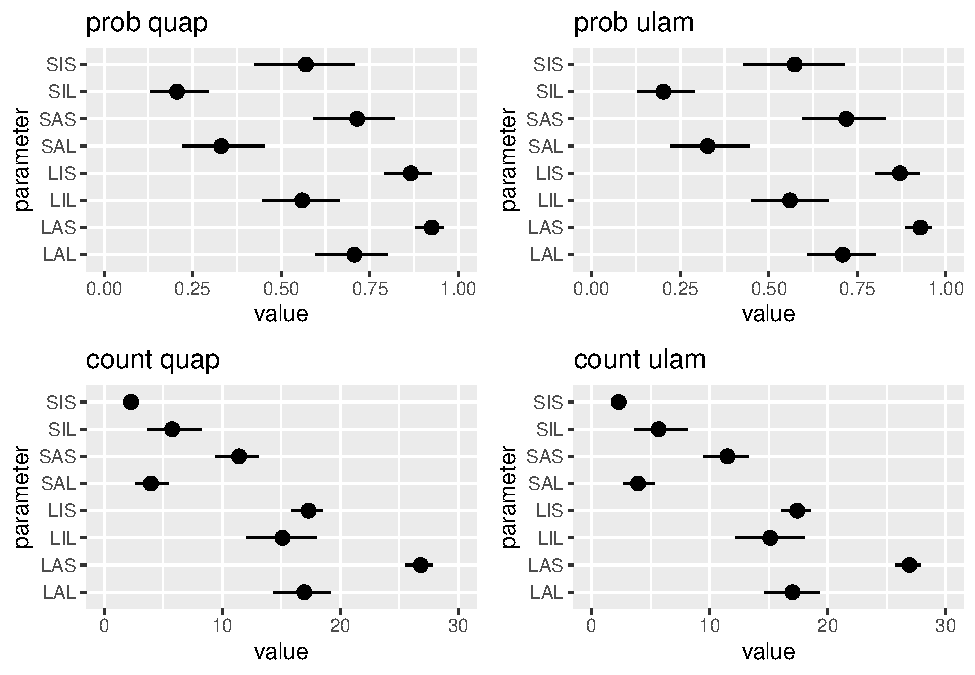
\includegraphics{03-sampling_imaginary_files/figure-latex/unnamed-chunk-23-1.pdf}

There were 49 girls born out of 100 births in the birth1 data. We know that these parents went on to have another child. Out of these 49 other children, our model expects the number of boys to be in the region of 27-28.

In reality there were 39 boys born after the birth of a girl, well outside the central expectations of the model.

No clue what's happening in the data. There's presumably some selection effect going on, but I can't think of a plausible one.

\hypertarget{further-reading-2}{%
\section*{Further Reading}\label{further-reading-2}}
\addcontentsline{toc}{section}{Further Reading}

\hypertarget{geocentric}{%
\chapter{Geocentric Models}\label{geocentric}}

\hypertarget{chapter-notes-3}{%
\section{Chapter Notes}\label{chapter-notes-3}}

I haven't written chapter notes for the first five chapters.

\hypertarget{questions-3}{%
\section{Questions}\label{questions-3}}

\hypertarget{e1-2}{%
\subsection*{4E1}\label{e1-2}}
\addcontentsline{toc}{subsection}{4E1}

\hypertarget{question-33}{%
\subsubsection*{Question}\label{question-33}}
\addcontentsline{toc}{subsubsection}{Question}

\begin{quote}
In the model definition below, which line is the likelihood?

\[
\begin{aligned}
y_i &\sim \text{Normal}(\mu, \sigma) \\
\mu &\sim \text{Normal}(0, 10) \\
\sigma &\sim \text{Exponential}(1)
\end{aligned}
\]
\end{quote}

\hypertarget{answer-33}{%
\subsubsection*{Answer}\label{answer-33}}
\addcontentsline{toc}{subsubsection}{Answer}

\(y_i ∼ \text{Normal}(µ, σ)\)

\hypertarget{e2-2}{%
\subsection*{4E2}\label{e2-2}}
\addcontentsline{toc}{subsection}{4E2}

\hypertarget{question-34}{%
\subsubsection*{Question}\label{question-34}}
\addcontentsline{toc}{subsubsection}{Question}

\begin{quote}
In the model definition just above, how many parameters are in the posterior distribution?
\end{quote}

\hypertarget{answer-34}{%
\subsubsection*{Answer}\label{answer-34}}
\addcontentsline{toc}{subsubsection}{Answer}

Two parameters, \(\mu\) \& \(\sigma\). \(y_i\) is not a parameter, it's the observed data.

\hypertarget{e3-2}{%
\subsection*{4E3}\label{e3-2}}
\addcontentsline{toc}{subsection}{4E3}

\hypertarget{question-35}{%
\subsubsection*{Question}\label{question-35}}
\addcontentsline{toc}{subsubsection}{Question}

\begin{quote}
Using the model definition above, write down the appropriate form of Bayes' theorem that includes the proper likelihood and priors.
\end{quote}

\hypertarget{answer-35}{%
\subsubsection*{Answer}\label{answer-35}}
\addcontentsline{toc}{subsubsection}{Answer}

In Bayes' theorem, we want to end up with the probability of some hypothesis, given some data. In this case, our hypotheses are values for parameters \(\mu\) and \(\sigma\). The probability of seeing the data (\(y_i\)) that we do comes from our likelihood, in this case we've assumed the data is the result of a normal distribution. Let's say we want to find the probability that our parameter values are \(\hat\mu\) and \(\hat\sigma\) given some piece of data \(y_i\). We apply Bayes' theorem like this:

\[
\begin{aligned}
P(\hat\mu,\hat\sigma | y_i) &= \frac{P(y_i | \hat\mu, \hat\sigma)P(\hat\mu)P(\hat\sigma)}{\int\int P(y_i | \mu, \sigma)P(\mu)P(\sigma) d\mu d\sigma}  \\
\\
                    &= \frac{N(y_i | \hat\mu, \hat\sigma)N(\hat\mu | 0,10)\text{Exp}(\hat\sigma|1)}{\int\int N(y_i | \mu, \sigma)N(\mu | 0,10)\text{Exp}(\sigma|1) d\mu d\sigma}
\end{aligned}
\]

I mean \(N(y_i | \mu, \sigma)\) to be read "the probability of observing \(y_i\) given that it is normally distributed with parameters \(\mu\) \& \(\sigma\). That notation is copied from page 78.

\hypertarget{e4-2}{%
\subsection*{4E4}\label{e4-2}}
\addcontentsline{toc}{subsection}{4E4}

\hypertarget{question-36}{%
\subsubsection*{Question}\label{question-36}}
\addcontentsline{toc}{subsubsection}{Question}

\begin{quote}
In the model definition below, which line is the linear model?

\[
\begin{aligned}
y_i &\sim \text{Normal}(\mu, \sigma) \\
\mu_i &= \alpha + \beta x_i \\
\alpha &\sim \text{Normal}(0, 10) \\ 
\beta &\sim \text{Normal}(0, 1) \\
\sigma &\sim \text{Exponential}(2) \\
\end{aligned}
\]
\end{quote}

\hypertarget{answer-36}{%
\subsubsection*{Answer}\label{answer-36}}
\addcontentsline{toc}{subsubsection}{Answer}

\(\mu_i = \alpha + \beta x_i\)

This is the assertion that \(\mu_i\) is a linear function of \(x_i\).

\hypertarget{e5-1}{%
\subsection*{4E5}\label{e5-1}}
\addcontentsline{toc}{subsection}{4E5}

\hypertarget{question-37}{%
\subsubsection*{Question}\label{question-37}}
\addcontentsline{toc}{subsubsection}{Question}

\begin{quote}
In the model definition just above, how many parameters are in the posterior distribution?
\end{quote}

\hypertarget{answer-37}{%
\subsubsection*{Answer}\label{answer-37}}
\addcontentsline{toc}{subsubsection}{Answer}

Three parameters, \(\alpha\), \(\beta\) \& \(\sigma\).

\hypertarget{m1-2}{%
\subsection*{4M1}\label{m1-2}}
\addcontentsline{toc}{subsection}{4M1}

\hypertarget{question-38}{%
\subsubsection*{Question}\label{question-38}}
\addcontentsline{toc}{subsubsection}{Question}

\begin{quote}
For the model definition below, simulate observed \(y\) values from the prior (not the posterior).

\[
\begin{aligned}
y_i &\sim \text{Normal}(\mu, \sigma) \\
\mu &\sim \text{Normal}(0, 10) \\
\sigma &\sim \text{Exponential}(1) \\
\end{aligned}
\]
\end{quote}

\hypertarget{answer-38}{%
\subsubsection*{Answer}\label{answer-38}}
\addcontentsline{toc}{subsubsection}{Answer}

\begin{Shaded}
\begin{Highlighting}[]
\NormalTok{num\_obs }\OtherTok{\textless{}{-}} \FloatTok{1e4}

\NormalTok{sim\_prior }\OtherTok{\textless{}{-}} \FunctionTok{rnorm}\NormalTok{(num\_obs,}
                   \AttributeTok{mean=}\FunctionTok{rnorm}\NormalTok{(num\_obs, }\AttributeTok{mean=}\DecValTok{0}\NormalTok{, }\AttributeTok{sd =} \DecValTok{10}\NormalTok{) , }
                   \AttributeTok{sd=}\FunctionTok{rexp}\NormalTok{(num\_obs, }\AttributeTok{rate =} \DecValTok{1}\NormalTok{))}

\FunctionTok{ggplot}\NormalTok{()}\SpecialCharTok{+}
  \FunctionTok{geom\_density}\NormalTok{(}\FunctionTok{aes}\NormalTok{(}\AttributeTok{x=}\NormalTok{sim\_prior))}
\end{Highlighting}
\end{Shaded}

\includegraphics{04-geocentric_files/figure-latex/unnamed-chunk-2-1.pdf}

\hypertarget{m2-2}{%
\subsection*{4M2}\label{m2-2}}
\addcontentsline{toc}{subsection}{4M2}

\hypertarget{question-39}{%
\subsubsection*{Question}\label{question-39}}
\addcontentsline{toc}{subsubsection}{Question}

\begin{quote}
Translate the model just above into a quap formula.
\end{quote}

\hypertarget{answer-39}{%
\subsubsection*{Answer}\label{answer-39}}
\addcontentsline{toc}{subsubsection}{Answer}

y \textasciitilde{} dnorm(mu, sigma)
mu \textasciitilde{} dnorm(0, 10)
sigma \textasciitilde{} dexp(1)

\hypertarget{m3-2}{%
\subsection*{4M3}\label{m3-2}}
\addcontentsline{toc}{subsection}{4M3}

\hypertarget{question-40}{%
\subsubsection*{Question}\label{question-40}}
\addcontentsline{toc}{subsubsection}{Question}

\begin{quote}
Translate the quap model formula below into a mathematical model definition.

y \textasciitilde{} dnorm( mu , sigma ),

mu \textless- a + b*x,

a \textasciitilde{} dnorm( 0 , 10 ),
.
b \textasciitilde{} dunif( 0 , 1 ),

sigma \textasciitilde{} dexp( 1 )
\end{quote}

\hypertarget{answer-40}{%
\subsubsection{Answer}\label{answer-40}}

\[
\begin{aligned}
y_i &\sim \text{Normal}(\mu, \sigma) \\
\mu_i &= \alpha + \beta x_i\\
\alpha &\sim  \text{Normal}(0, 10) \\
\beta & \sim \text{Uniform}(0,1) \\
\sigma & \sim \text{Exponential}(1)
\end{aligned}
\]

\hypertarget{m4-2}{%
\subsection*{4M4}\label{m4-2}}
\addcontentsline{toc}{subsection}{4M4}

\hypertarget{question-41}{%
\subsubsection*{Question}\label{question-41}}
\addcontentsline{toc}{subsubsection}{Question}

\begin{quote}
A sample of students is measured for height each year for 3 years. After the third year, you want to fit a linear regression predicting height using year as a predictor.

Write down the mathematical model definition for this regression, using any variable names and priors you choose. Be prepared to defend your choice of priors.
\end{quote}

\hypertarget{answer-41}{%
\subsubsection*{Answer}\label{answer-41}}
\addcontentsline{toc}{subsubsection}{Answer}

hi ∼ Normal(µ, σ)

µi = α + βyi

α \textasciitilde{} Normal(178, 20)

β ∼ Normal(0,10)

σ ∼ Exponential(0.05)

\hypertarget{m5-2}{%
\subsection*{4M5}\label{m5-2}}
\addcontentsline{toc}{subsection}{4M5}

\hypertarget{question-42}{%
\subsubsection*{Question}\label{question-42}}
\addcontentsline{toc}{subsubsection}{Question}

\begin{quote}
Now suppose I remind you that every student got taller each year. Does this information lead you to change your choice of priors? How?
\end{quote}

\hypertarget{answer-42}{%
\subsubsection*{Answer}\label{answer-42}}
\addcontentsline{toc}{subsubsection}{Answer}

Yes, I would revise β to something like β ∼ Exponential(0.2).

Now it can only be positive (before I wasn't sure if we were following the same students, or the same class with a new intake of students).

Probably still anticipating too much height growth with this prior, assuming these are university students. On the other hand Dennis Rodman grew like 8 inches one summer after high school apparently so want to keep open the possibility.

\hypertarget{m6-2}{%
\subsection*{4M6}\label{m6-2}}
\addcontentsline{toc}{subsection}{4M6}

\hypertarget{question-43}{%
\subsubsection*{Question}\label{question-43}}
\addcontentsline{toc}{subsubsection}{Question}

\begin{quote}
Now suppose I tell you that the variance among heights for students of the same age is never more than 64cm. How does this lead you to revise your priors?
\end{quote}

\hypertarget{answer-43}{%
\subsubsection*{Answer}\label{answer-43}}
\addcontentsline{toc}{subsubsection}{Answer}

I think my previous prior σ ∼ Exponential(0.05) is probably still fine. If anything this question makes me think I wasn't being conservative enough with my first choice of priors.

\hypertarget{m7-1}{%
\subsection*{4M7}\label{m7-1}}
\addcontentsline{toc}{subsection}{4M7}

\hypertarget{question-44}{%
\subsubsection*{Question}\label{question-44}}
\addcontentsline{toc}{subsubsection}{Question}

\begin{quote}
Refit model m4.3 from the chapter, but omit the mean weight xbar this time.
Compare the new model's posterior to that of the original model. In particular, look at the covariance among the
parameters. What is different? Then compare the posterior predictions of both models.
\end{quote}

\hypertarget{answer-44}{%
\subsubsection*{Answer}\label{answer-44}}
\addcontentsline{toc}{subsubsection}{Answer}

\begin{Shaded}
\begin{Highlighting}[]
\FunctionTok{data}\NormalTok{(Howell1)}

\NormalTok{d }\OtherTok{\textless{}{-}}\NormalTok{ Howell1 }

\NormalTok{d2 }\OtherTok{\textless{}{-}}\NormalTok{ d[ d}\SpecialCharTok{$}\NormalTok{age }\SpecialCharTok{\textgreater{}=} \DecValTok{18}\NormalTok{ , ]}

\CommentTok{\# define the average weight, x{-}bar }

\NormalTok{xbar }\OtherTok{\textless{}{-}} \FunctionTok{mean}\NormalTok{(d2}\SpecialCharTok{$}\NormalTok{weight)}

\CommentTok{\# fit model}

\FunctionTok{set.seed}\NormalTok{(}\DecValTok{100}\NormalTok{)}
\NormalTok{m4}\FloatTok{.3} \OtherTok{\textless{}{-}} \FunctionTok{quap}\NormalTok{( }\FunctionTok{alist}\NormalTok{(}
\NormalTok{  height }\SpecialCharTok{\textasciitilde{}} \FunctionTok{dnorm}\NormalTok{( mu , sigma ) , }
\NormalTok{  mu }\OtherTok{\textless{}{-}}\NormalTok{ a }\SpecialCharTok{+}\NormalTok{ b}\SpecialCharTok{*}\NormalTok{( weight }\SpecialCharTok{{-}}\NormalTok{ xbar ) , }
\NormalTok{  a }\SpecialCharTok{\textasciitilde{}} \FunctionTok{dnorm}\NormalTok{( }\DecValTok{178}\NormalTok{ , }\DecValTok{20}\NormalTok{ ) , }
\NormalTok{  b }\SpecialCharTok{\textasciitilde{}} \FunctionTok{dlnorm}\NormalTok{( }\DecValTok{0}\NormalTok{ , }\DecValTok{1}\NormalTok{ ) , }
\NormalTok{  sigma }\SpecialCharTok{\textasciitilde{}} \FunctionTok{dunif}\NormalTok{( }\DecValTok{0}\NormalTok{ , }\DecValTok{50}\NormalTok{ )}
\NormalTok{  ) , }
  \AttributeTok{data=}\NormalTok{d2 )}

\FunctionTok{set.seed}\NormalTok{(}\DecValTok{100}\NormalTok{)}
\NormalTok{m4.}\FloatTok{3.2} \OtherTok{\textless{}{-}} \FunctionTok{quap}\NormalTok{( }\FunctionTok{alist}\NormalTok{(}
\NormalTok{  height }\SpecialCharTok{\textasciitilde{}} \FunctionTok{dnorm}\NormalTok{( mu , sigma ) , }
\NormalTok{  mu }\OtherTok{\textless{}{-}}\NormalTok{ a }\SpecialCharTok{+}\NormalTok{ b}\SpecialCharTok{*}\NormalTok{( weight ) , }
\NormalTok{  a }\SpecialCharTok{\textasciitilde{}} \FunctionTok{dnorm}\NormalTok{( }\DecValTok{178}\NormalTok{ , }\DecValTok{20}\NormalTok{ ) , }
\NormalTok{  b }\SpecialCharTok{\textasciitilde{}} \FunctionTok{dlnorm}\NormalTok{( }\DecValTok{0}\NormalTok{ , }\DecValTok{1}\NormalTok{ ) , }
\NormalTok{  sigma }\SpecialCharTok{\textasciitilde{}} \FunctionTok{dunif}\NormalTok{( }\DecValTok{0}\NormalTok{ , }\DecValTok{50}\NormalTok{ )}
\NormalTok{  ) , }
  \AttributeTok{data=}\NormalTok{d2 )}
\end{Highlighting}
\end{Shaded}

Chapter questions unfinished.

\hypertarget{further-reading-3}{%
\section*{Further Reading}\label{further-reading-3}}
\addcontentsline{toc}{section}{Further Reading}

\hypertarget{many_variables}{%
\chapter{The Many Variables \& The Spurious Waffles}\label{many_variables}}

\hypertarget{chapter-notes-4}{%
\section{Chapter Notes}\label{chapter-notes-4}}

I haven't written chapter notes for the first five chapters.

\hypertarget{questions-4}{%
\section{Questions}\label{questions-4}}

\hypertarget{e1-3}{%
\subsection*{5E1}\label{e1-3}}
\addcontentsline{toc}{subsection}{5E1}

\hypertarget{question-45}{%
\subsubsection*{Question}\label{question-45}}
\addcontentsline{toc}{subsubsection}{Question}

\begin{quote}
Which of the linear models below are multiple linear regressions?

\begin{enumerate}
\def\labelenumi{(\arabic{enumi})}
\item
  µi = α + βxi
\item
  µi = βx * xi + βz * zi
\item
  µi = α + β(xi − zi)
\item
  µi = α + βx * xi + βz * zi
\end{enumerate}
\end{quote}

\hypertarget{answer-45}{%
\subsubsection*{Answer}\label{answer-45}}
\addcontentsline{toc}{subsubsection}{Answer}

Number 4 looks the most like the multiple regressions in the chapter: µ is regressed on both xi and zi with the ``intercept'' α. (2) is just (4) with the α set to zero, so that counts too.

Number 1 is just a bivariate regression.

Number 3 is interesting. I think this is not really a multiple regression, even though there are two variables. Rather than attempting to determine separately the influence of x and z on µ, you are asserting in the model that they have and equal and opposite impact. I think this is not really what you want a multiple regression to do, but don't feel confident about my answer.

\hypertarget{e2-3}{%
\subsection*{5E2}\label{e2-3}}
\addcontentsline{toc}{subsection}{5E2}

\hypertarget{question-46}{%
\subsubsection*{Question}\label{question-46}}
\addcontentsline{toc}{subsubsection}{Question}

\begin{quote}
Write down a multiple regression to evaluate the claim:

Animal diversity is linearly related to latitude, but only after controlling for plant diversity. You just need to write down the model definition.
\end{quote}

\hypertarget{answer-46}{%
\subsubsection*{Answer}\label{answer-46}}
\addcontentsline{toc}{subsubsection}{Answer}

Oh boy. This question immediately feels like a trap with ``animal diversity is \emph{linearly} related to latitude.'' Surely if I choose to use a multiple linear regression with two variables, and control for one, the only relationships I'll observe will be linear.

I'm going to ignore the ``linearly'' part of the question from this point. It seems like the claim is that if I naively regress animal diversity on to latitude without accounting for plant diversity, I would find no relationship. I.e. that the relationship between latitude and animal diversity is masked.

If that interpretation is correct, I would start with a bivariate model.

\$\$
A\_i \sim Normal(\mu, \sigma) \textbackslash{}

\mu\_i = \alpha + \beta\_L*L
\$\$

Where if the claim is true I would expect to see little relationship. I would then move on to a multiple regression including plant diversity:

\$\$
A\_i \sim Normal(\mu, \sigma) \textbackslash{}

\mu\_i = \alpha + \beta\_L*L +\beta\_P * P
\$\$

and examine whether it appears as if a relationship has now emerged.

\hypertarget{e3-3}{%
\subsection*{5E3}\label{e3-3}}
\addcontentsline{toc}{subsection}{5E3}

\hypertarget{question-47}{%
\subsubsection*{Question}\label{question-47}}
\addcontentsline{toc}{subsubsection}{Question}

\begin{quote}
Write down a multiple regression to evaluate the claim: Neither amount of funding nor size of laboratory is by itself a good predictor of time to PhD degree; but together these variables are both positively associated with time to degree.

Write down the model definition and indicate which side of zero each slope parameter should be on.
\end{quote}

\hypertarget{answer-47}{%
\subsubsection*{Answer}\label{answer-47}}
\addcontentsline{toc}{subsubsection}{Answer}

\$\$
T\_i \sim Normal(\mu, \sigma) \textbackslash{}

\mu\_i = \alpha + \beta\_F*F +\beta\_S * S
\$\$

T - time to PhD degree
F - amount of funding
S - size of laboratory

\hypertarget{e4-3}{%
\subsection*{5E4}\label{e4-3}}
\addcontentsline{toc}{subsection}{5E4}

\hypertarget{question-48}{%
\subsubsection*{Question}\label{question-48}}
\addcontentsline{toc}{subsubsection}{Question}

\begin{quote}
Suppose you have a single categorical predictor with 4 levels (unique values), labeled A, B, C and D. Let \(A_i\) be an indicator variable that is 1 where case i is in category A. Also suppose \(B_i\), \(C_i\), and \(D_i\) for the other categories.
Now which of the following linear models are inferentially equivalent ways to include the categorical variable in a regression? Models are inferentially equivalent when it's possible to compute one posterior distribution from the posterior distribution of another model.

\[
(1) \mu_i = \alpha + \beta_A A_i + \beta_B B_i + \beta_D D_i  \\
(2) \mu_i = \alpha + \beta_A A_i + \beta_B B_i + \beta_C C_i + \beta_D D_i \\ 
(3) \mu_i = \alpha + \beta_B B_i + \beta_C C_i + \beta_D D_i \\
(4) \mu_i = \alpha_A A_i + α_B B_i + α_C C_i + α_D D_i \\
(5) \mu_i = \alpha_A(1 − B_i − C_i −D_i) + \alpha_B B_i + \alpha_C C_i + \alpha_D D_i
\]
\end{quote}

\hypertarget{answer-48}{%
\subsubsection*{Answer}\label{answer-48}}
\addcontentsline{toc}{subsubsection}{Answer}

1 is the standard indicator variable approach. Where A, B and D are equal to 0, \(\alpha\) is the mean \(\mu\) where the predictor is at level C.
2 There is redundancy in two, surely it wouldn't be possible to estimate \(\alpha\) - it can take any value and produce the same \(\mu\) so long as the appropriate \(\beta_x\) adjusts to compensate. I don't know if that means it is not inferentially equivalent though.
3 is clearly equivalent to (1), it doesn't make a difference (except for interpretation) which of the levels you label null.
4 Is equivalent also, just set \(\alpha_c\) equal to \(\alpha\) from (1).
5 Is an incredibly annoying way to set up your model, but can be pretty easily transformed into (3) with some algebra and relabelling:

\[
\begin{aligned}
\mu_i &= \alpha_A(1 − B_i − C_i −D_i) + \alpha_B B_i + \alpha_C C_i + \alpha_D D_i \\
&= \alpha_A + (\alpha_B-\alpha_A)B_i + (\alpha_C -\alpha_A)C_i +(\alpha_D-\alpha_A)D_i  \\
&= \alpha + \beta_B B_i + \beta_C C_i + \beta_D D_i
\end{aligned}          
\]

\hypertarget{further-reading-4}{%
\section*{Further Reading}\label{further-reading-4}}
\addcontentsline{toc}{section}{Further Reading}

\hypertarget{haunted_dag}{%
\chapter{The Haunted DAG \& The Causal Terror}\label{haunted_dag}}

\hypertarget{chapter-notes-5}{%
\section{Chapter Notes}\label{chapter-notes-5}}

Figure 6.1 Selection Bias

\includegraphics{06-haunted_dag_files/figure-latex/unnamed-chunk-2-1.pdf}

Parameters estimates for effect of leg length on height.

\includegraphics{06-haunted_dag_files/figure-latex/unnamed-chunk-3-1.pdf}

Figure 6.2 Posterior of height\textasciitilde leg Model

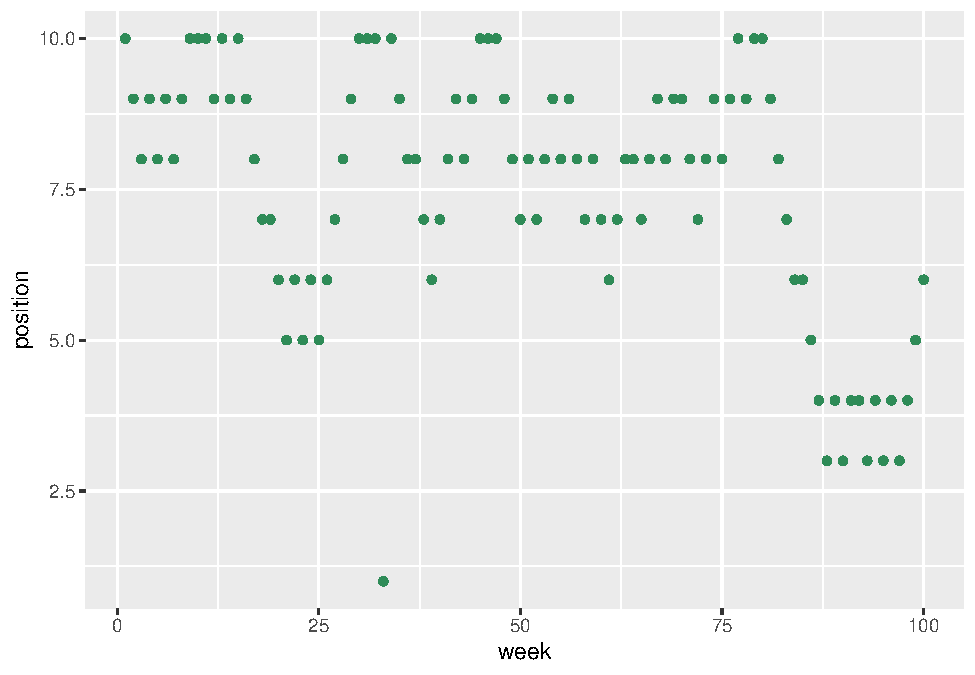
\includegraphics{06-haunted_dag_files/figure-latex/unnamed-chunk-4-1.pdf} 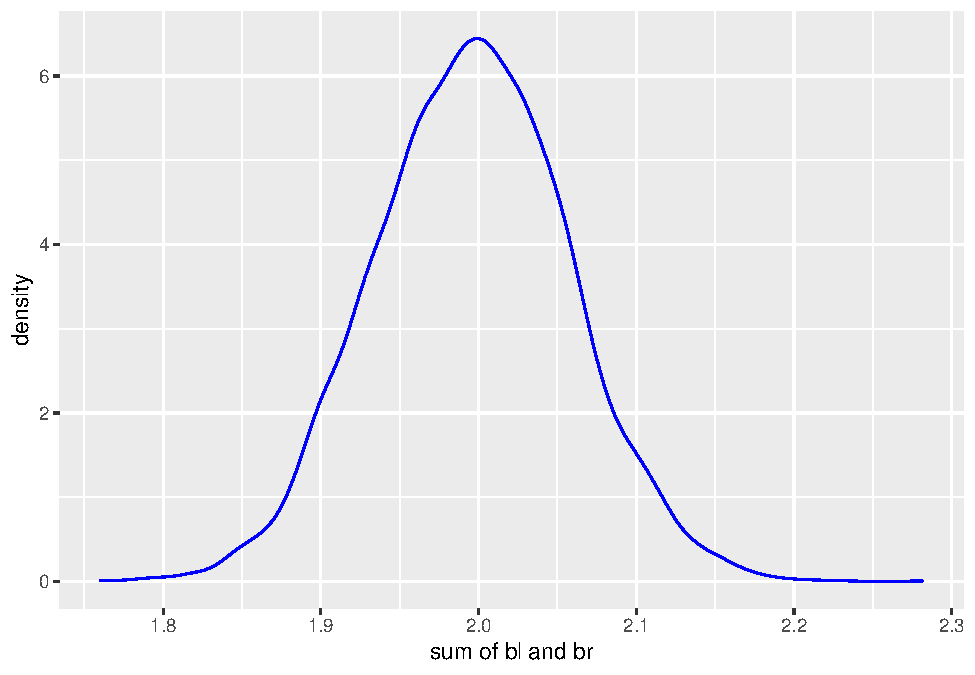
\includegraphics{06-haunted_dag_files/figure-latex/unnamed-chunk-4-2.pdf}

Figure 6.3

\includegraphics{06-haunted_dag_files/figure-latex/unnamed-chunk-5-1.pdf}

Primate Milk DAG

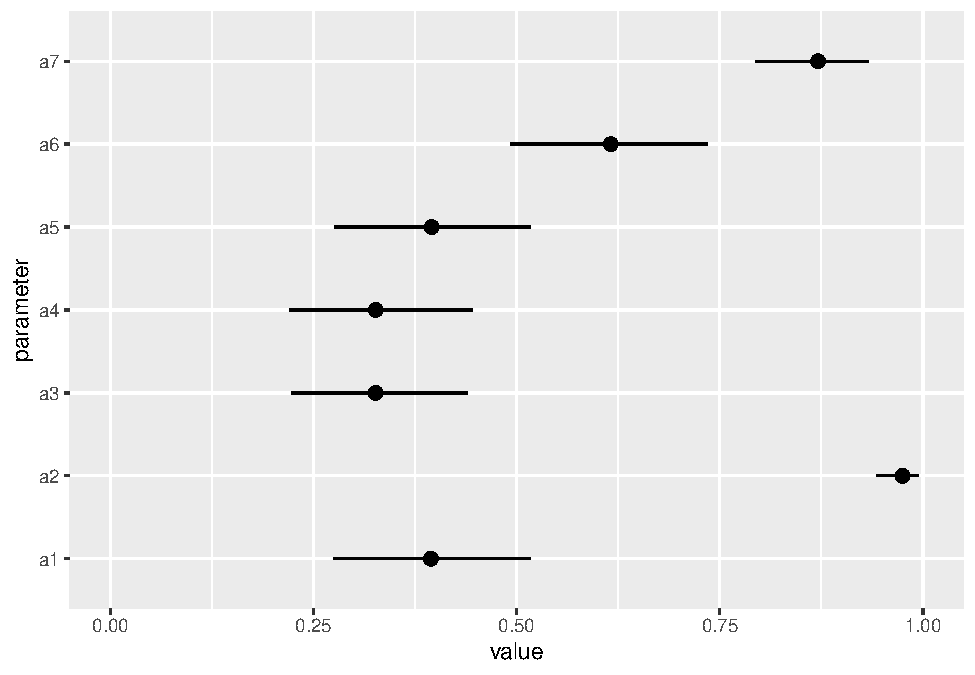
\includegraphics{06-haunted_dag_files/figure-latex/unnamed-chunk-6-1.pdf}

Simulating Colliinearity

\includegraphics{06-haunted_dag_files/figure-latex/unnamed-chunk-7-1.pdf}

\includegraphics{06-haunted_dag_files/figure-latex/unnamed-chunk-8-1.pdf} 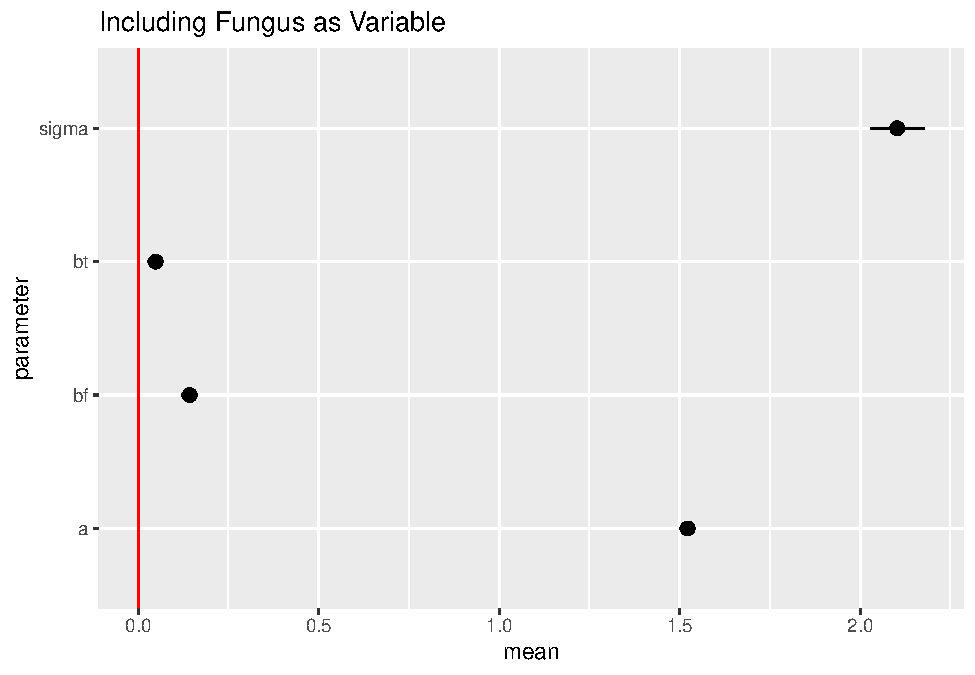
\includegraphics{06-haunted_dag_files/figure-latex/unnamed-chunk-8-2.pdf} 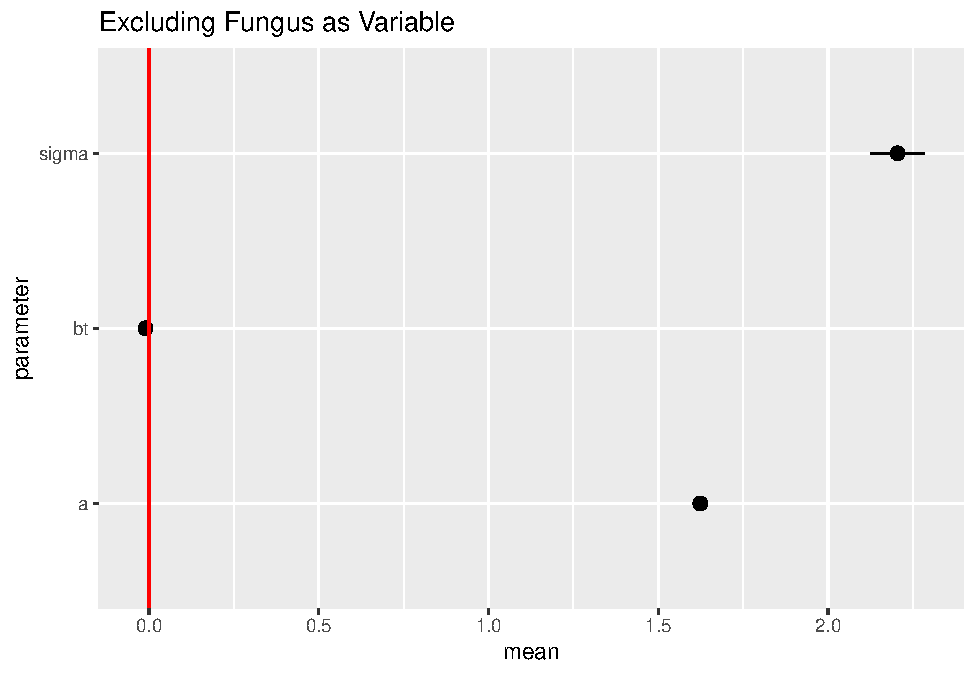
\includegraphics{06-haunted_dag_files/figure-latex/unnamed-chunk-8-3.pdf}

Here's my very rough attempt at explaining to myself why conditioning on fungus makes treatment appear to have a small positive effect.

If fungus is present we may have:

\begin{itemize}
\tightlist
\item
  treatment present and moisture present
\item
  treatment absent and moisture either way (leaning towards present)
\end{itemize}

If fungus is absent we may have:

\begin{itemize}
\tightlist
\item
  treatment absent and moisture absent
\item
  treatment present and moisture either way (leaning towards absent)
\end{itemize}

So once we know fungus there is a weak positive correlation between treatment and moisture. Since moisture is good for plant growth, this means a positive relationship between treatment and growth.

\hypertarget{questions-5}{%
\section{Questions}\label{questions-5}}

\hypertarget{e1-4}{%
\subsection*{6E1}\label{e1-4}}
\addcontentsline{toc}{subsection}{6E1}

\hypertarget{question-49}{%
\subsubsection*{Question}\label{question-49}}
\addcontentsline{toc}{subsubsection}{Question}

\begin{quote}
List three mechanisms by which multiple regression can produce false inferences about causal effects.
\end{quote}

\hypertarget{answer-49}{%
\subsubsection*{Answer}\label{answer-49}}
\addcontentsline{toc}{subsubsection}{Answer}

\begin{enumerate}
\def\labelenumi{\arabic{enumi}.}
\item
  Multicollinearity - regression on highly correlated predictors can produce misleading parameters, as in the leg, or primate milk examples.
\item
  Post-treatment bias - regression on post-treatment effects can make it appear that the treatment is not effective, as in the fungus example.
\item
  Collider bias - regression on a collider can create the appearance of an association between two variables that does not exist.
\end{enumerate}

\hypertarget{e3-4}{%
\subsection*{6E3}\label{e3-4}}
\addcontentsline{toc}{subsection}{6E3}

\hypertarget{question-50}{%
\subsubsection*{Question}\label{question-50}}
\addcontentsline{toc}{subsubsection}{Question}

\begin{quote}
List the four elemental confounds. Can you explain the conditional dependencies of each?
\end{quote}

\hypertarget{answer-50}{%
\subsubsection*{Answer}\label{answer-50}}
\addcontentsline{toc}{subsubsection}{Answer}

\begin{enumerate}
\def\labelenumi{\arabic{enumi}.}
\tightlist
\item
  Fork - X and Y are independent, once we condition on Z.
\end{enumerate}

\includegraphics{06-haunted_dag_files/figure-latex/unnamed-chunk-9-1.pdf}

\begin{enumerate}
\def\labelenumi{\arabic{enumi}.}
\setcounter{enumi}{1}
\tightlist
\item
  Pipe - X and Y are independent, once we condition on Z.
\end{enumerate}

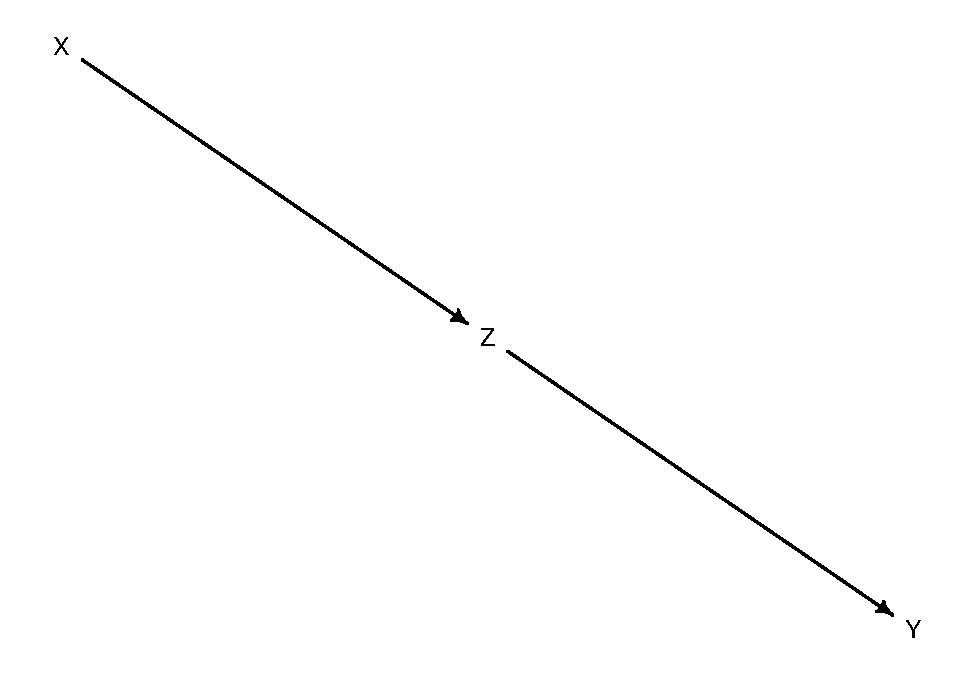
\includegraphics{06-haunted_dag_files/figure-latex/unnamed-chunk-10-1.pdf}

\begin{enumerate}
\def\labelenumi{\arabic{enumi}.}
\setcounter{enumi}{2}
\tightlist
\item
  Collider - Conditioning on Z creates an association between X and Y.
\end{enumerate}

\includegraphics{06-haunted_dag_files/figure-latex/unnamed-chunk-11-1.pdf}

\begin{enumerate}
\def\labelenumi{\arabic{enumi}.}
\setcounter{enumi}{3}
\tightlist
\item
  Descendant - Conditioning on D partly conditions on Z.
\end{enumerate}

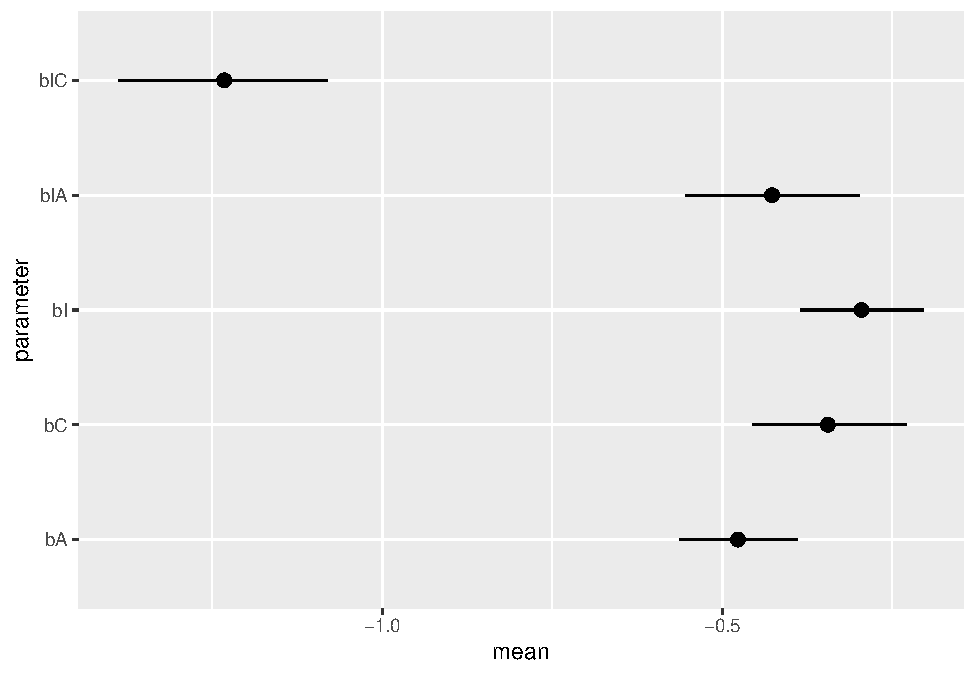
\includegraphics{06-haunted_dag_files/figure-latex/unnamed-chunk-12-1.pdf}

\hypertarget{e4-4}{%
\subsection*{6E4}\label{e4-4}}
\addcontentsline{toc}{subsection}{6E4}

\hypertarget{question-51}{%
\subsubsection*{Question}\label{question-51}}
\addcontentsline{toc}{subsubsection}{Question}

\begin{quote}
How is a biased sample like conditioning on a collider? Think of the example at the open of the chapter.
\end{quote}

\hypertarget{answer-51}{%
\subsubsection*{Answer}\label{answer-51}}
\addcontentsline{toc}{subsubsection}{Answer}

Using the publishing example at the beginning of the chapter, we know that there is no causal relationship between trustworthiness and newsworthiness (because that's how the simulation is constructed). However, both cause selection for publication, creating a collider. We saw that sampling only the published papers created a negative correlation between the two predictors.

Conditioning on publication would have the same effect - once we know newsworthiness and publication status, we can deduce some information about trustworthiness, or vice versa. For example, a study that was published but had low newsworthiness must be quite trustworthy. A study with high trustworthiness that wasn't published is probably not very newsworthy.

Conditioning on the collider has the same result as only sampling from papers that were published: the creation of a spurious association.

\hypertarget{m1-3}{%
\subsection*{6M1}\label{m1-3}}
\addcontentsline{toc}{subsection}{6M1}

\hypertarget{question-52}{%
\subsubsection*{Question}\label{question-52}}
\addcontentsline{toc}{subsubsection}{Question}

\begin{quote}
Modify the DAG on page 186 to include the variable V, an unobserved cause of C and Y: C ← V→ Y. Reanalyze the DAG. How many paths connect X to Y? Which must be closed? Which variables should you condition on now?
\end{quote}

\hypertarget{answer-52}{%
\subsubsection*{Answer}\label{answer-52}}
\addcontentsline{toc}{subsubsection}{Answer}

Here's the original DAG:

\includegraphics{06-haunted_dag_files/figure-latex/unnamed-chunk-13-1.pdf}

Now we add the unobserved V:

\includegraphics{06-haunted_dag_files/figure-latex/unnamed-chunk-14-1.pdf}

Previously, we could condition on either A or C to find the direct casual effect of X on Y. Now C is a collider, so we should condition on A.

The dagitty package corrobates this:

\begin{Shaded}
\begin{Highlighting}[]
\FunctionTok{adjustmentSets}\NormalTok{( dag\_6M1B , }\AttributeTok{exposure=}\StringTok{"X"}\NormalTok{ , }\AttributeTok{outcome=}\StringTok{"Y"}\NormalTok{ )}
\end{Highlighting}
\end{Shaded}

\begin{verbatim}
## { A }
\end{verbatim}

\hypertarget{m2-3}{%
\subsection*{6M2}\label{m2-3}}
\addcontentsline{toc}{subsection}{6M2}

\hypertarget{question-53}{%
\subsubsection*{Question}\label{question-53}}
\addcontentsline{toc}{subsubsection}{Question}

\begin{quote}
Sometimes, in order to avoid multicollinearity, people inspect pairwise correlations among predictors before including them in a model. This is a bad procedure, because what matters is the conditional association, not the association before the variables are included in the model. To highlight this, consider the DAG X → Z → Y. Simulate data from this DAG so that the correlation between X and Z is very large. Then include both in a model predicting Y.

Do you observe any multicollinearity? Why or why not? What is different from the legs example in the chapter?
\end{quote}

\hypertarget{answer-53}{%
\subsubsection*{Answer}\label{answer-53}}
\addcontentsline{toc}{subsubsection}{Answer}

Modifying the leg example:

\begin{Shaded}
\begin{Highlighting}[]
\NormalTok{N }\OtherTok{\textless{}{-}} \DecValTok{1000} 
\FunctionTok{set.seed}\NormalTok{(}\DecValTok{909}\NormalTok{) }

\NormalTok{Y }\OtherTok{\textless{}{-}} \FunctionTok{rnorm}\NormalTok{(N,}\DecValTok{10}\NormalTok{,}\DecValTok{2}\NormalTok{)}
\NormalTok{Y\_prop }\OtherTok{\textless{}{-}} \FunctionTok{runif}\NormalTok{(N,}\FloatTok{0.4}\NormalTok{,}\FloatTok{0.5}\NormalTok{) }

\NormalTok{Z }\OtherTok{\textless{}{-}}\NormalTok{ Y\_prop}\SpecialCharTok{*}\NormalTok{Y }\SpecialCharTok{+} \FunctionTok{rnorm}\NormalTok{( N , }\DecValTok{0}\NormalTok{ , }\FloatTok{0.02}\NormalTok{ )}
\NormalTok{Z\_prop }\OtherTok{\textless{}{-}} \FunctionTok{runif}\NormalTok{(N,}\FloatTok{0.8}\NormalTok{,}\FloatTok{0.9}\NormalTok{) }

\NormalTok{X }\OtherTok{\textless{}{-}} \SpecialCharTok{{-}}\NormalTok{Z\_prop}\SpecialCharTok{*}\NormalTok{Z }\SpecialCharTok{+} \FunctionTok{rnorm}\NormalTok{( N , }\DecValTok{0}\NormalTok{ , }\FloatTok{0.02}\NormalTok{ )}

\NormalTok{data\_6M2 }\OtherTok{\textless{}{-}} \FunctionTok{bind\_cols}\NormalTok{(}\AttributeTok{X=}\NormalTok{X,}\AttributeTok{Z=}\NormalTok{Z,}\AttributeTok{Y=}\NormalTok{Y)}

\FunctionTok{ggpairs}\NormalTok{(data\_6M2)}
\end{Highlighting}
\end{Shaded}

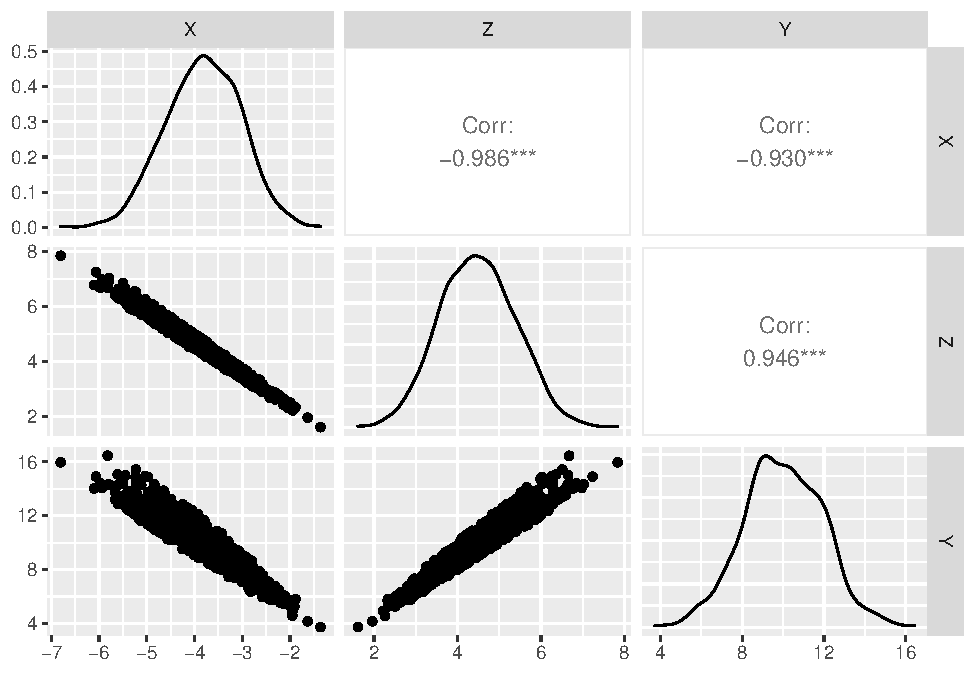
\includegraphics{06-haunted_dag_files/figure-latex/unnamed-chunk-16-1.pdf}

\begin{Shaded}
\begin{Highlighting}[]
\FunctionTok{set.seed}\NormalTok{(}\DecValTok{100}\NormalTok{)}
\NormalTok{m6M2 }\OtherTok{\textless{}{-}} \FunctionTok{quap}\NormalTok{( }
  \FunctionTok{alist}\NormalTok{(}
\NormalTok{    Y }\SpecialCharTok{\textasciitilde{}} \FunctionTok{dnorm}\NormalTok{( mu , sigma ) , }
\NormalTok{    mu }\OtherTok{\textless{}{-}}\NormalTok{ a }\SpecialCharTok{+}\NormalTok{ bX}\SpecialCharTok{*}\NormalTok{X }\SpecialCharTok{+}\NormalTok{ bZ}\SpecialCharTok{*}\NormalTok{Z , }
\NormalTok{    a }\SpecialCharTok{\textasciitilde{}} \FunctionTok{dnorm}\NormalTok{( }\DecValTok{10}\NormalTok{ , }\DecValTok{100}\NormalTok{ ) , }
\NormalTok{    bX }\SpecialCharTok{\textasciitilde{}} \FunctionTok{dnorm}\NormalTok{( }\SpecialCharTok{{-}}\DecValTok{3}\NormalTok{ , }\DecValTok{10}\NormalTok{ ) , }
\NormalTok{    bZ }\SpecialCharTok{\textasciitilde{}} \FunctionTok{dnorm}\NormalTok{( }\DecValTok{2}\NormalTok{ , }\DecValTok{10}\NormalTok{ ) , }
\NormalTok{    sigma }\SpecialCharTok{\textasciitilde{}} \FunctionTok{dexp}\NormalTok{( }\DecValTok{1}\NormalTok{ )}
\NormalTok{) , }\AttributeTok{data=}\NormalTok{data\_6M2 )}


\FunctionTok{ggplot}\NormalTok{(}\AttributeTok{data=}\FunctionTok{precis}\NormalTok{(m6M2))}\SpecialCharTok{+}
  \FunctionTok{geom\_pointrange}\NormalTok{(}\FunctionTok{aes}\NormalTok{(}\AttributeTok{x=}\FunctionTok{rownames}\NormalTok{(}\FunctionTok{precis}\NormalTok{(m6M2)),}\AttributeTok{y=}\NormalTok{mean,}\AttributeTok{ymin=}\StringTok{\textasciigrave{}}\AttributeTok{5.5\%}\StringTok{\textasciigrave{}}\NormalTok{,}\AttributeTok{ymax=}\StringTok{\textasciigrave{}}\AttributeTok{94.5\%}\StringTok{\textasciigrave{}}\NormalTok{))}\SpecialCharTok{+}
  \FunctionTok{geom\_hline}\NormalTok{(}\AttributeTok{yintercept =} \DecValTok{0}\NormalTok{,}\AttributeTok{col=}\StringTok{"red"}\NormalTok{)}\SpecialCharTok{+}
  \FunctionTok{xlab}\NormalTok{(}\StringTok{"parameter"}\NormalTok{)}\SpecialCharTok{+}
  \FunctionTok{coord\_flip}\NormalTok{()}
\end{Highlighting}
\end{Shaded}

\begin{verbatim}
## Warning in sqrt(diag(vcov(model))): NaNs produced

## Warning in sqrt(diag(vcov(model))): NaNs produced

## Warning in sqrt(diag(vcov(model))): NaNs produced

## Warning in sqrt(diag(vcov(model))): NaNs produced

## Warning in sqrt(diag(vcov(model))): NaNs produced

## Warning in sqrt(diag(vcov(model))): NaNs produced

## Warning in sqrt(diag(vcov(model))): NaNs produced

## Warning in sqrt(diag(vcov(model))): NaNs produced

## Warning in sqrt(diag(vcov(model))): NaNs produced
\end{verbatim}

\begin{verbatim}
## Warning: Removed 1 rows containing missing values (geom_segment).
\end{verbatim}

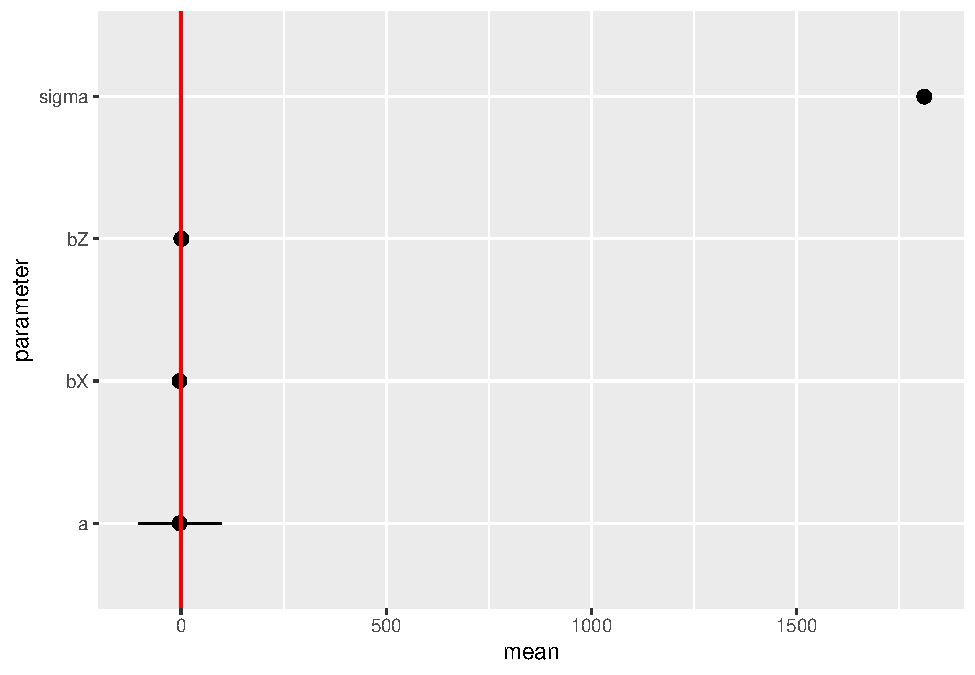
\includegraphics{06-haunted_dag_files/figure-latex/unnamed-chunk-16-2.pdf}

In the legs example, the model was very uncertain about the parameter values for both legs. This is not the case here, the parameter estimate for the influence of Z is about as expected, 2-2.5. The model has correctly identified that the only influence of X on Y is through Z, and so produces parameter estimates for X much smaller than expected. We have a pipe, and including Z blocks the path from X to Y, but we don't have the problems with identifiability that we had in the legs example.

There is no way to tell this scenario apart from the legs example simply from looking at the pairwise correlations.

\hypertarget{m3-3}{%
\subsection*{6M3}\label{m3-3}}
\addcontentsline{toc}{subsection}{6M3}

\hypertarget{question-54}{%
\subsubsection*{Question}\label{question-54}}
\addcontentsline{toc}{subsubsection}{Question}

\begin{quote}
Learning to analyze DAGs requires practice. For each of the four DAGs below, state which variables, if any, you must adjust for (condition on) to estimate the total causal influence of X on Y.
\end{quote}

\hypertarget{answer-54}{%
\subsubsection*{Answer}\label{answer-54}}
\addcontentsline{toc}{subsubsection}{Answer}

\begin{enumerate}
\def\labelenumi{\arabic{enumi}.}
\tightlist
\item
  We should condition on Z to block the backdoor path.
\end{enumerate}

\begin{Shaded}
\begin{Highlighting}[]
\FunctionTok{drawdag}\NormalTok{(dag\_6M3}\FloatTok{.1}\NormalTok{)}
\end{Highlighting}
\end{Shaded}

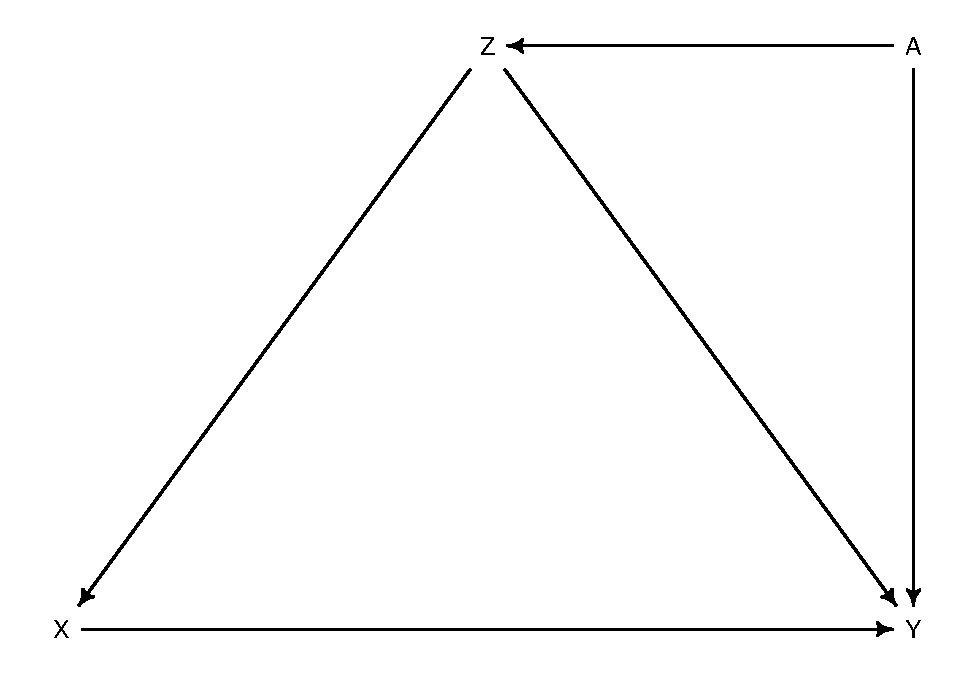
\includegraphics{06-haunted_dag_files/figure-latex/unnamed-chunk-18-1.pdf}

\begin{Shaded}
\begin{Highlighting}[]
\FunctionTok{adjustmentSets}\NormalTok{(dag\_6M3}\FloatTok{.1}\NormalTok{,}\AttributeTok{exposure =} \StringTok{"X"}\NormalTok{,}\AttributeTok{outcome =} \StringTok{"Y"}\NormalTok{,}\AttributeTok{effect =} \StringTok{"total"}\NormalTok{)}
\end{Highlighting}
\end{Shaded}

\begin{verbatim}
## { Z }
\end{verbatim}

\begin{enumerate}
\def\labelenumi{\arabic{enumi}.}
\setcounter{enumi}{1}
\tightlist
\item
  We no longer want to condition on Z - it is a collider.
\end{enumerate}

\begin{Shaded}
\begin{Highlighting}[]
\FunctionTok{drawdag}\NormalTok{(dag\_6M3}\FloatTok{.2}\NormalTok{)}
\end{Highlighting}
\end{Shaded}

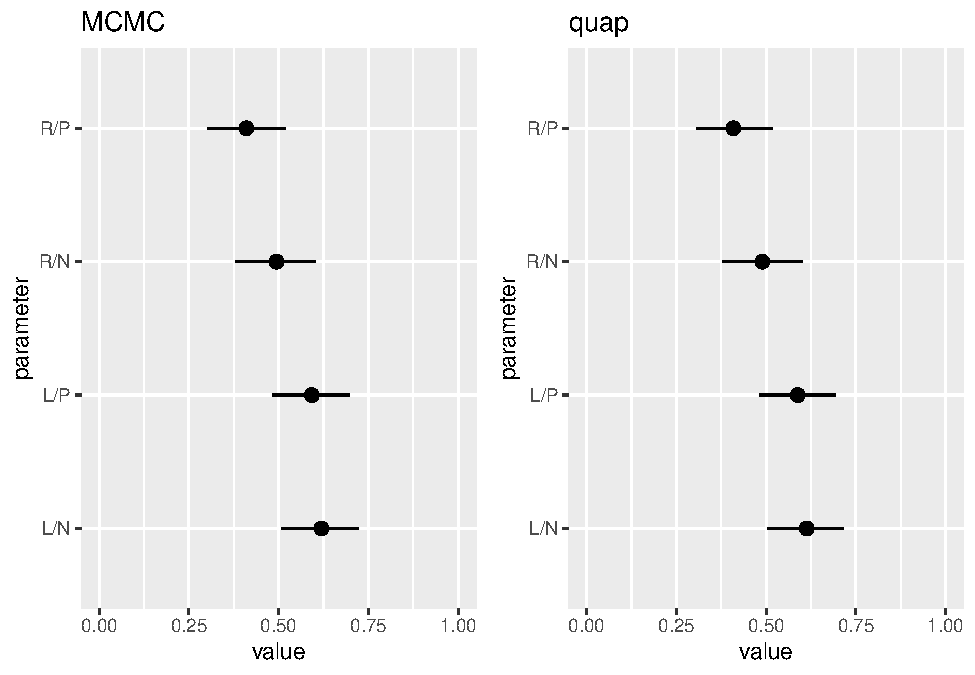
\includegraphics{06-haunted_dag_files/figure-latex/unnamed-chunk-19-1.pdf}

\begin{Shaded}
\begin{Highlighting}[]
\FunctionTok{adjustmentSets}\NormalTok{(dag\_6M3}\FloatTok{.2}\NormalTok{,}\AttributeTok{exposure =} \StringTok{"X"}\NormalTok{,}\AttributeTok{outcome =} \StringTok{"Y"}\NormalTok{,}\AttributeTok{effect =} \StringTok{"total"}\NormalTok{)}
\end{Highlighting}
\end{Shaded}

\begin{verbatim}
##  {}
\end{verbatim}

\begin{enumerate}
\def\labelenumi{\arabic{enumi}.}
\setcounter{enumi}{2}
\tightlist
\item
  We no longer want to condition on Z - it is a collider.
\end{enumerate}

\begin{Shaded}
\begin{Highlighting}[]
\FunctionTok{drawdag}\NormalTok{(dag\_6M3}\FloatTok{.3}\NormalTok{)}
\end{Highlighting}
\end{Shaded}

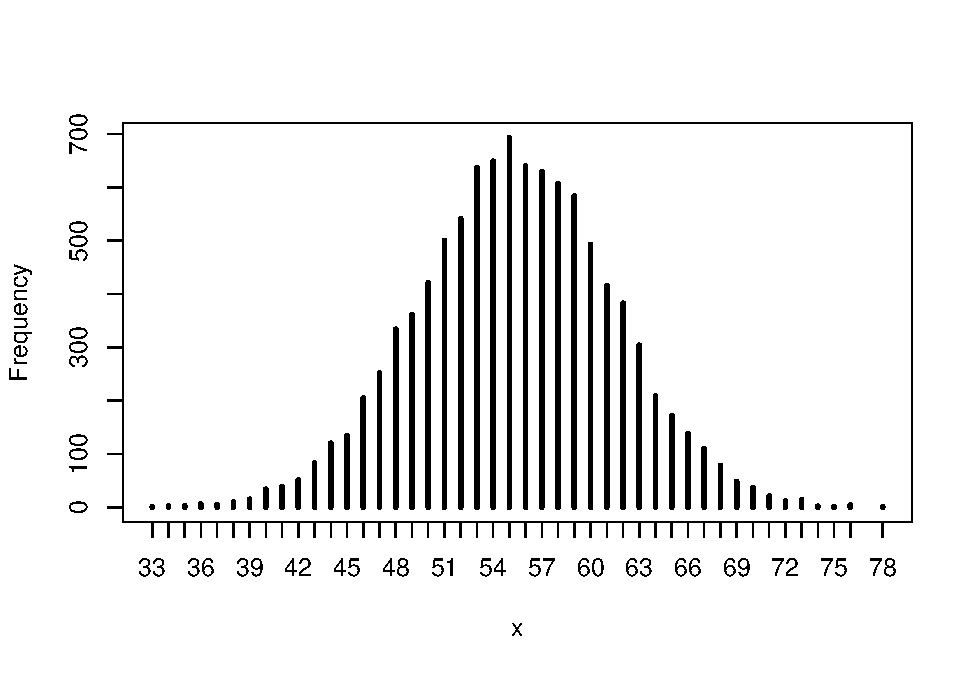
\includegraphics{06-haunted_dag_files/figure-latex/unnamed-chunk-20-1.pdf}

\begin{Shaded}
\begin{Highlighting}[]
\FunctionTok{adjustmentSets}\NormalTok{(dag\_6M3}\FloatTok{.3}\NormalTok{,}\AttributeTok{exposure =} \StringTok{"X"}\NormalTok{,}\AttributeTok{outcome =} \StringTok{"Y"}\NormalTok{,}\AttributeTok{effect =} \StringTok{"total"}\NormalTok{)}
\end{Highlighting}
\end{Shaded}

\begin{verbatim}
##  {}
\end{verbatim}

\begin{enumerate}
\def\labelenumi{\arabic{enumi}.}
\setcounter{enumi}{3}
\tightlist
\item
  We don't want to condition on Z here because we are looking for the \emph{total} casual influence of X on Y - one route of this influence goes through Z. We should condition on A however, to block the backdoor path.
\end{enumerate}

\begin{Shaded}
\begin{Highlighting}[]
\FunctionTok{drawdag}\NormalTok{(dag\_6M3}\FloatTok{.4}\NormalTok{)}
\end{Highlighting}
\end{Shaded}

\includegraphics{06-haunted_dag_files/figure-latex/unnamed-chunk-21-1.pdf}

\begin{Shaded}
\begin{Highlighting}[]
\FunctionTok{adjustmentSets}\NormalTok{(dag\_6M3}\FloatTok{.4}\NormalTok{,}\AttributeTok{exposure =} \StringTok{"X"}\NormalTok{,}\AttributeTok{outcome =} \StringTok{"Y"}\NormalTok{,}\AttributeTok{effect =} \StringTok{"total"}\NormalTok{)}
\end{Highlighting}
\end{Shaded}

\begin{verbatim}
## { A }
\end{verbatim}

\hypertarget{h1-2}{%
\subsection*{6H1}\label{h1-2}}
\addcontentsline{toc}{subsection}{6H1}

\hypertarget{question-55}{%
\subsubsection*{Question}\label{question-55}}
\addcontentsline{toc}{subsubsection}{Question}

\begin{quote}
Use the Waffle House data to find the total causal influence of number of Waffle Houses on divorce rate. Justify your model or models with a causal graph.
\end{quote}

\hypertarget{answer-55}{%
\subsubsection*{Answer}\label{answer-55}}
\addcontentsline{toc}{subsubsection}{Answer}

Looking through the available variables, I think I want to consider the following:
* Number of Waffle Houses (W)
* Divorce rate (D)
* Whether we're in the South (S)
* Marriage rate (M)
* Median age of marriage (A)

Here's my proposed DAG:

\begin{Shaded}
\begin{Highlighting}[]
\NormalTok{dag\_waf }\OtherTok{\textless{}{-}} \FunctionTok{dagitty}\NormalTok{( }\StringTok{"dag \{S {-}\textgreater{} W; S {-}\textgreater{} M; S{-}\textgreater{}A; W {-}\textgreater{} D ; M {-}\textgreater{} D; A {-}\textgreater{} D;\}"}\NormalTok{)}
\FunctionTok{coordinates}\NormalTok{(dag\_waf) }\OtherTok{\textless{}{-}} \FunctionTok{list}\NormalTok{( }\AttributeTok{x=}\FunctionTok{c}\NormalTok{(}\AttributeTok{W=}\DecValTok{0}\NormalTok{,}\AttributeTok{S=}\DecValTok{1}\NormalTok{,}\AttributeTok{M=}\DecValTok{1}\NormalTok{,}\AttributeTok{D=}\DecValTok{1}\NormalTok{,}\AttributeTok{A=}\DecValTok{2}\NormalTok{) , }\AttributeTok{y=}\FunctionTok{c}\NormalTok{(}\AttributeTok{S=}\DecValTok{0}\NormalTok{,}\AttributeTok{W=}\DecValTok{1}\NormalTok{,}\AttributeTok{M=}\DecValTok{1}\NormalTok{,}\AttributeTok{A=}\DecValTok{1}\NormalTok{,}\AttributeTok{D=}\DecValTok{2}\NormalTok{) )}

\FunctionTok{drawdag}\NormalTok{(dag\_waf )}
\end{Highlighting}
\end{Shaded}

\includegraphics{06-haunted_dag_files/figure-latex/unnamed-chunk-22-1.pdf}

\begin{Shaded}
\begin{Highlighting}[]
\FunctionTok{adjustmentSets}\NormalTok{(dag\_waf,}\AttributeTok{exposure =} \StringTok{"W"}\NormalTok{,}\AttributeTok{outcome =} \StringTok{"D"}\NormalTok{,}\AttributeTok{effect =} \StringTok{"total"}\NormalTok{)}
\end{Highlighting}
\end{Shaded}

\begin{verbatim}
## { A, M }
## { S }
\end{verbatim}

So we need to include S in the model, to block the backdoor path through A and M.

After loading the data, standardising, and doing some prior simulation, I have the model below:

\begin{Shaded}
\begin{Highlighting}[]
\FunctionTok{set.seed}\NormalTok{(}\DecValTok{100}\NormalTok{)}
\NormalTok{m6H1 }\OtherTok{\textless{}{-}} \FunctionTok{quap}\NormalTok{( }
  \FunctionTok{alist}\NormalTok{(}
\NormalTok{    Divorce }\SpecialCharTok{\textasciitilde{}} \FunctionTok{dnorm}\NormalTok{( mu , sigma ) , }
\NormalTok{    mu }\OtherTok{\textless{}{-}}\NormalTok{ a[South] }\SpecialCharTok{+}\NormalTok{ bW}\SpecialCharTok{*}\NormalTok{WaffleHouses, }
\NormalTok{    a[South] }\SpecialCharTok{\textasciitilde{}} \FunctionTok{dnorm}\NormalTok{( }\DecValTok{0}\NormalTok{ , }\FloatTok{0.6}\NormalTok{ ) , }
\NormalTok{    bW }\SpecialCharTok{\textasciitilde{}} \FunctionTok{dnorm}\NormalTok{( }\DecValTok{0}\NormalTok{ , }\FloatTok{0.2}\NormalTok{ ) , }
\NormalTok{    sigma }\SpecialCharTok{\textasciitilde{}} \FunctionTok{dexp}\NormalTok{( }\DecValTok{1}\NormalTok{ )}
\NormalTok{) , }\AttributeTok{data=}\NormalTok{data\_waf )}


\FunctionTok{ggplot}\NormalTok{(}\AttributeTok{data=}\FunctionTok{precis}\NormalTok{(m6H1,}\AttributeTok{depth =} \DecValTok{2}\NormalTok{))}\SpecialCharTok{+}
  \FunctionTok{geom\_pointrange}\NormalTok{(}\FunctionTok{aes}\NormalTok{(}\AttributeTok{x=}\FunctionTok{rownames}\NormalTok{(}\FunctionTok{precis}\NormalTok{(m6H1,}\AttributeTok{depth =} \DecValTok{2}\NormalTok{)),}\AttributeTok{y=}\NormalTok{mean,}\AttributeTok{ymin=}\StringTok{\textasciigrave{}}\AttributeTok{5.5\%}\StringTok{\textasciigrave{}}\NormalTok{,}\AttributeTok{ymax=}\StringTok{\textasciigrave{}}\AttributeTok{94.5\%}\StringTok{\textasciigrave{}}\NormalTok{))}\SpecialCharTok{+}
  \FunctionTok{geom\_hline}\NormalTok{(}\AttributeTok{yintercept =} \DecValTok{0}\NormalTok{,}\AttributeTok{col=}\StringTok{"red"}\NormalTok{)}\SpecialCharTok{+}
  \FunctionTok{xlab}\NormalTok{(}\StringTok{"parameter"}\NormalTok{)}\SpecialCharTok{+}
  \FunctionTok{coord\_flip}\NormalTok{()}
\end{Highlighting}
\end{Shaded}

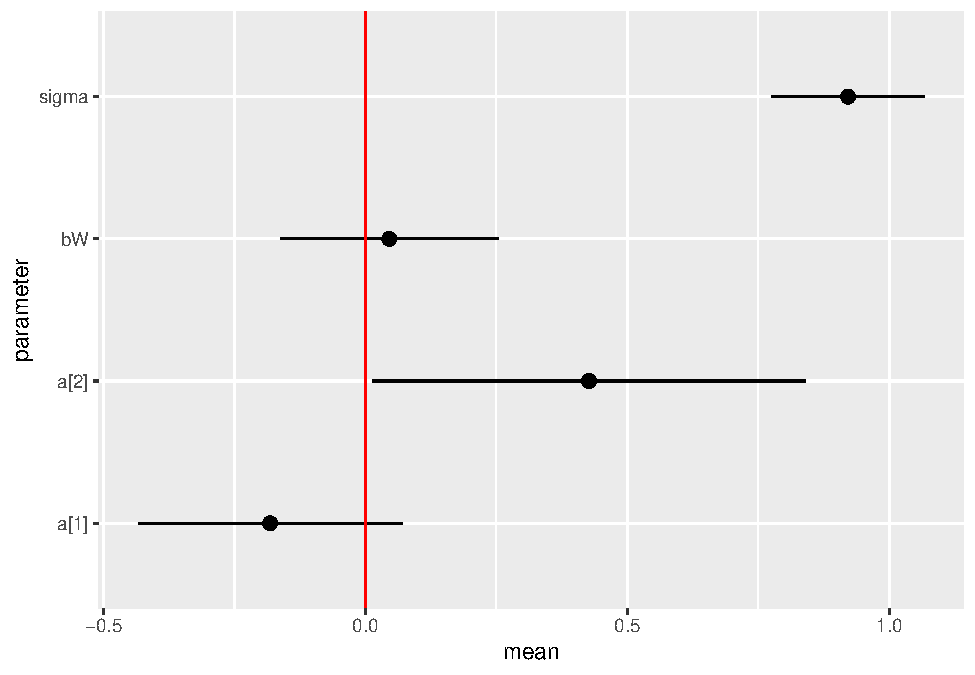
\includegraphics{06-haunted_dag_files/figure-latex/unnamed-chunk-24-1.pdf}

This is consistent with the number of Waffle Houses having no causal effect on the divorce rate.

\hypertarget{h2-2}{%
\subsection*{6H2}\label{h2-2}}
\addcontentsline{toc}{subsection}{6H2}

\hypertarget{question-56}{%
\subsubsection*{Question}\label{question-56}}
\addcontentsline{toc}{subsubsection}{Question}

\begin{quote}
Build a series of models to test the implied conditional independencies of the causal graph you used in the previous problem. If any of the tests fail, how do you think the graph needs to be amended?

Does the graph need more or fewer arrows? Feel free to nominate variables that aren't in the data.
\end{quote}

\hypertarget{answer-56}{%
\subsubsection*{Answer}\label{answer-56}}
\addcontentsline{toc}{subsubsection}{Answer}

\begin{Shaded}
\begin{Highlighting}[]
\FunctionTok{impliedConditionalIndependencies}\NormalTok{(dag\_waf)}
\end{Highlighting}
\end{Shaded}

\begin{verbatim}
## A _||_ M | S
## A _||_ W | S
## D _||_ S | A, M, W
## M _||_ W | S
\end{verbatim}

We'll first test that the divorce rate is independent of being in the South, conditional on number of waffle houses, median age of marriage, and marriage rate.

\begin{Shaded}
\begin{Highlighting}[]
\FunctionTok{set.seed}\NormalTok{(}\DecValTok{100}\NormalTok{)}
\NormalTok{m6H2}\FloatTok{.1} \OtherTok{\textless{}{-}} \FunctionTok{quap}\NormalTok{( }
  \FunctionTok{alist}\NormalTok{(}
\NormalTok{    Divorce }\SpecialCharTok{\textasciitilde{}} \FunctionTok{dnorm}\NormalTok{( mu , sigma ) , }
\NormalTok{    mu }\OtherTok{\textless{}{-}}\NormalTok{ a[South] }\SpecialCharTok{+}\NormalTok{ bW}\SpecialCharTok{*}\NormalTok{WaffleHouses }\SpecialCharTok{+}\NormalTok{ bM}\SpecialCharTok{*}\NormalTok{Marriage }\SpecialCharTok{+}\NormalTok{ bA}\SpecialCharTok{*}\NormalTok{MedianAgeMarriage, }
\NormalTok{    a[South] }\SpecialCharTok{\textasciitilde{}} \FunctionTok{dnorm}\NormalTok{( }\DecValTok{0}\NormalTok{ , }\FloatTok{0.6}\NormalTok{ ) , }
\NormalTok{    bW }\SpecialCharTok{\textasciitilde{}} \FunctionTok{dnorm}\NormalTok{( }\DecValTok{0}\NormalTok{ , }\FloatTok{0.2}\NormalTok{ ) , }
\NormalTok{    bM }\SpecialCharTok{\textasciitilde{}} \FunctionTok{dnorm}\NormalTok{( }\DecValTok{0}\NormalTok{ , }\DecValTok{1}\NormalTok{ ) ,}
\NormalTok{    bA }\SpecialCharTok{\textasciitilde{}} \FunctionTok{dnorm}\NormalTok{( }\DecValTok{0}\NormalTok{ , }\DecValTok{1}\NormalTok{ ) ,}
\NormalTok{    sigma }\SpecialCharTok{\textasciitilde{}} \FunctionTok{dexp}\NormalTok{( }\DecValTok{1}\NormalTok{ )}
\NormalTok{) , }\AttributeTok{data=}\NormalTok{data\_waf )}

\NormalTok{m6H2}\FloatTok{.1}\NormalTok{\_post }\OtherTok{\textless{}{-}}\NormalTok{ post }\OtherTok{\textless{}{-}} \FunctionTok{extract.samples}\NormalTok{(m6H2}\FloatTok{.1}\NormalTok{)}
\NormalTok{m6H2}\FloatTok{.1}\NormalTok{\_post}\SpecialCharTok{$}\NormalTok{diff\_south }\OtherTok{\textless{}{-}}\NormalTok{ m6H2}\FloatTok{.1}\NormalTok{\_post}\SpecialCharTok{$}\NormalTok{a[,}\DecValTok{1}\NormalTok{] }\SpecialCharTok{{-}}\NormalTok{ m6H2}\FloatTok{.1}\NormalTok{\_post}\SpecialCharTok{$}\NormalTok{a[,}\DecValTok{2}\NormalTok{]}

\FunctionTok{ggplot}\NormalTok{(}\AttributeTok{data=}\FunctionTok{precis}\NormalTok{( m6H2}\FloatTok{.1}\NormalTok{\_post , }\AttributeTok{depth=}\DecValTok{2}\NormalTok{ ))}\SpecialCharTok{+}
  \FunctionTok{geom\_pointrange}\NormalTok{(}\FunctionTok{aes}\NormalTok{(}\AttributeTok{x=}\FunctionTok{rownames}\NormalTok{(}\FunctionTok{precis}\NormalTok{( m6H2}\FloatTok{.1}\NormalTok{\_post , }\AttributeTok{depth=}\DecValTok{2}\NormalTok{ )),}\AttributeTok{y=}\NormalTok{mean,}\AttributeTok{ymin=}\StringTok{\textasciigrave{}}\AttributeTok{5.5\%}\StringTok{\textasciigrave{}}\NormalTok{,}\AttributeTok{ymax=}\StringTok{\textasciigrave{}}\AttributeTok{94.5\%}\StringTok{\textasciigrave{}}\NormalTok{))}\SpecialCharTok{+}
  \FunctionTok{geom\_hline}\NormalTok{(}\AttributeTok{yintercept =} \DecValTok{0}\NormalTok{,}\AttributeTok{col=}\StringTok{"red"}\NormalTok{)}\SpecialCharTok{+}
  \FunctionTok{xlab}\NormalTok{(}\StringTok{"parameter"}\NormalTok{)}\SpecialCharTok{+}
  \FunctionTok{coord\_flip}\NormalTok{()}
\end{Highlighting}
\end{Shaded}

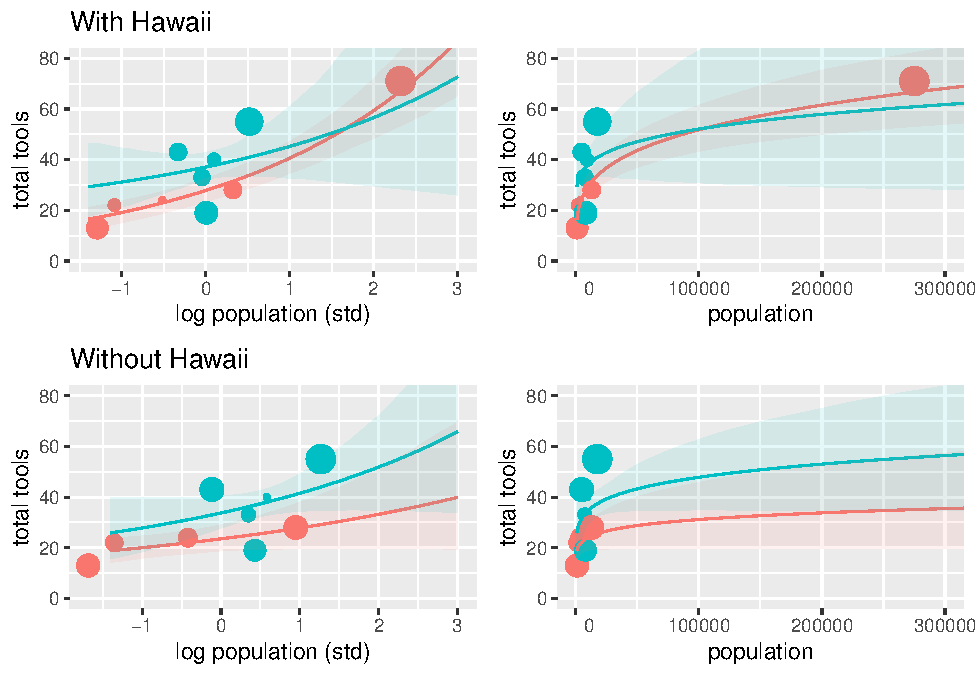
\includegraphics{06-haunted_dag_files/figure-latex/unnamed-chunk-26-1.pdf}

The values of the diff\_south parameter are consistent with the conditional independence, but I'm not completely happy that I've caught all the ways that being in the South can influence the divorce rate. Perhaps I should add an arrow directly from the South to the divorce rate, or add in an unobserved variable to stand in for cultural/ religious attitudes towards divorce.

We'll test one more conditional independence, one that I think is more likely to be true. Let's see if the median age of marriage is independent of the number of waffle houses, once we condition on being in the south.

\begin{Shaded}
\begin{Highlighting}[]
\FunctionTok{set.seed}\NormalTok{(}\DecValTok{100}\NormalTok{)}
\NormalTok{m6H2}\FloatTok{.2} \OtherTok{\textless{}{-}} \FunctionTok{quap}\NormalTok{( }
  \FunctionTok{alist}\NormalTok{(}
\NormalTok{    MedianAgeMarriage }\SpecialCharTok{\textasciitilde{}} \FunctionTok{dnorm}\NormalTok{( mu , sigma ) , }
\NormalTok{    mu }\OtherTok{\textless{}{-}}\NormalTok{ a[South] }\SpecialCharTok{+}\NormalTok{ bW}\SpecialCharTok{*}\NormalTok{WaffleHouses, }
\NormalTok{    a[South] }\SpecialCharTok{\textasciitilde{}} \FunctionTok{dnorm}\NormalTok{( }\DecValTok{0}\NormalTok{ , }\FloatTok{0.6}\NormalTok{ ) , }
\NormalTok{    bW }\SpecialCharTok{\textasciitilde{}} \FunctionTok{dnorm}\NormalTok{( }\DecValTok{0}\NormalTok{ , }\DecValTok{1}\NormalTok{ ) , }
\NormalTok{    sigma }\SpecialCharTok{\textasciitilde{}} \FunctionTok{dexp}\NormalTok{( }\DecValTok{1}\NormalTok{ )}
\NormalTok{) , }\AttributeTok{data=}\NormalTok{data\_waf )}

\NormalTok{m6H2}\FloatTok{.2}\NormalTok{\_post }\OtherTok{\textless{}{-}} \FunctionTok{extract.samples}\NormalTok{(m6H2}\FloatTok{.2}\NormalTok{)}
\NormalTok{m6H2}\FloatTok{.2}\NormalTok{\_post}\SpecialCharTok{$}\NormalTok{diff\_south }\OtherTok{\textless{}{-}}\NormalTok{ m6H2}\FloatTok{.2}\NormalTok{\_post}\SpecialCharTok{$}\NormalTok{a[,}\DecValTok{1}\NormalTok{] }\SpecialCharTok{{-}}\NormalTok{ m6H2}\FloatTok{.2}\NormalTok{\_post}\SpecialCharTok{$}\NormalTok{a[,}\DecValTok{2}\NormalTok{]}

\FunctionTok{ggplot}\NormalTok{(}\AttributeTok{data=}\FunctionTok{precis}\NormalTok{( m6H2}\FloatTok{.2}\NormalTok{\_post , }\AttributeTok{depth=}\DecValTok{2}\NormalTok{ ))}\SpecialCharTok{+}
  \FunctionTok{geom\_pointrange}\NormalTok{(}\FunctionTok{aes}\NormalTok{(}\AttributeTok{x=}\FunctionTok{rownames}\NormalTok{(}\FunctionTok{precis}\NormalTok{( m6H2}\FloatTok{.2}\NormalTok{\_post , }\AttributeTok{depth=}\DecValTok{2}\NormalTok{ )),}\AttributeTok{y=}\NormalTok{mean,}\AttributeTok{ymin=}\StringTok{\textasciigrave{}}\AttributeTok{5.5\%}\StringTok{\textasciigrave{}}\NormalTok{,}\AttributeTok{ymax=}\StringTok{\textasciigrave{}}\AttributeTok{94.5\%}\StringTok{\textasciigrave{}}\NormalTok{))}\SpecialCharTok{+}
  \FunctionTok{geom\_hline}\NormalTok{(}\AttributeTok{yintercept =} \DecValTok{0}\NormalTok{,}\AttributeTok{col=}\StringTok{"red"}\NormalTok{)}\SpecialCharTok{+}
  \FunctionTok{xlab}\NormalTok{(}\StringTok{"parameter"}\NormalTok{)}\SpecialCharTok{+}
  \FunctionTok{coord\_flip}\NormalTok{()}
\end{Highlighting}
\end{Shaded}

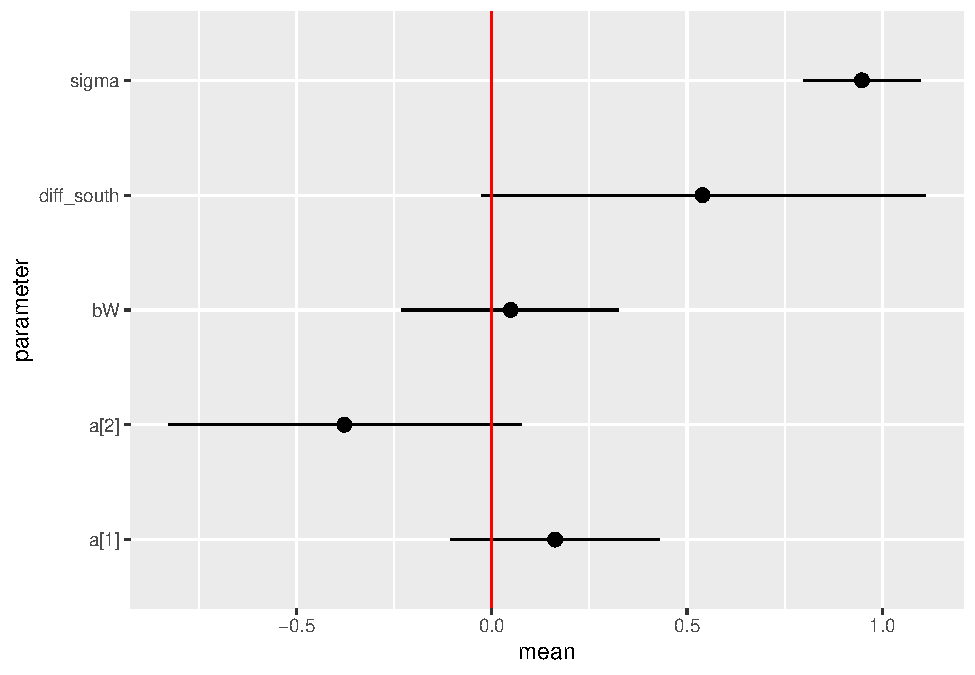
\includegraphics{06-haunted_dag_files/figure-latex/unnamed-chunk-27-1.pdf}

The parameter bW is estimated to be quite close to zero.

\hypertarget{h3-2}{%
\subsection*{6H3}\label{h3-2}}
\addcontentsline{toc}{subsection}{6H3}

\hypertarget{question-57}{%
\subsubsection*{Question}\label{question-57}}
\addcontentsline{toc}{subsubsection}{Question}

\begin{quote}
Use a model to infer the total causal influence of area on weight. Would increasing the area available to each fox make it heavier (healthier)?

You might want to standardize the variables. Regardless, use prior predictive simulation to show that your model's prior predictions stay within the possible outcome range.
\end{quote}

\hypertarget{answer-57}{%
\subsubsection*{Answer}\label{answer-57}}
\addcontentsline{toc}{subsubsection}{Answer}

We don't need to condition on any other parameters since we're looking for the total causal effect.

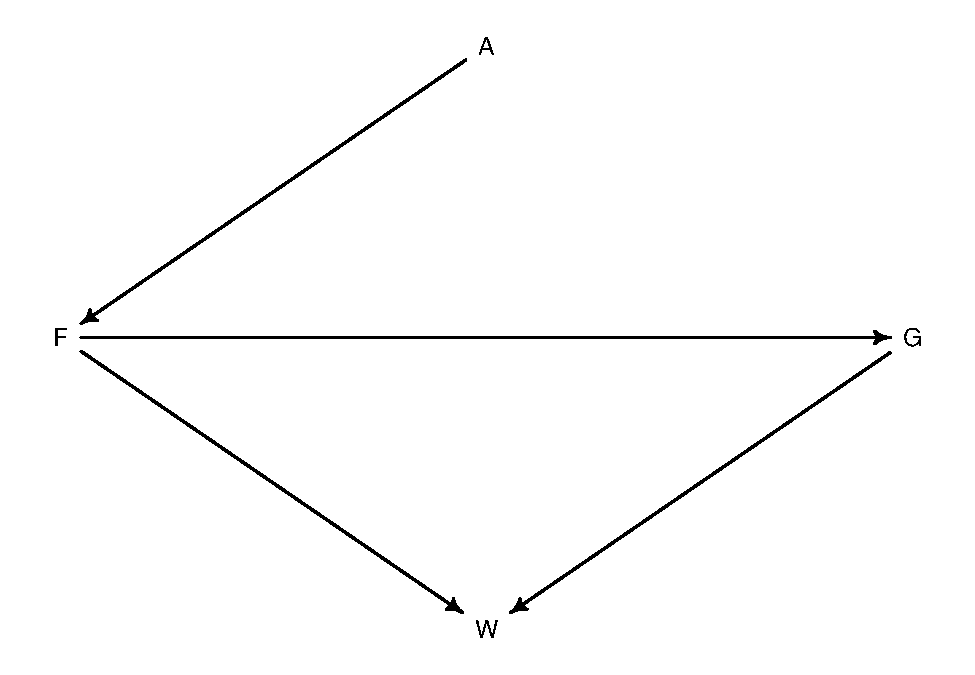
\includegraphics{06-haunted_dag_files/figure-latex/unnamed-chunk-28-1.pdf}

\begin{verbatim}
##  {}
\end{verbatim}

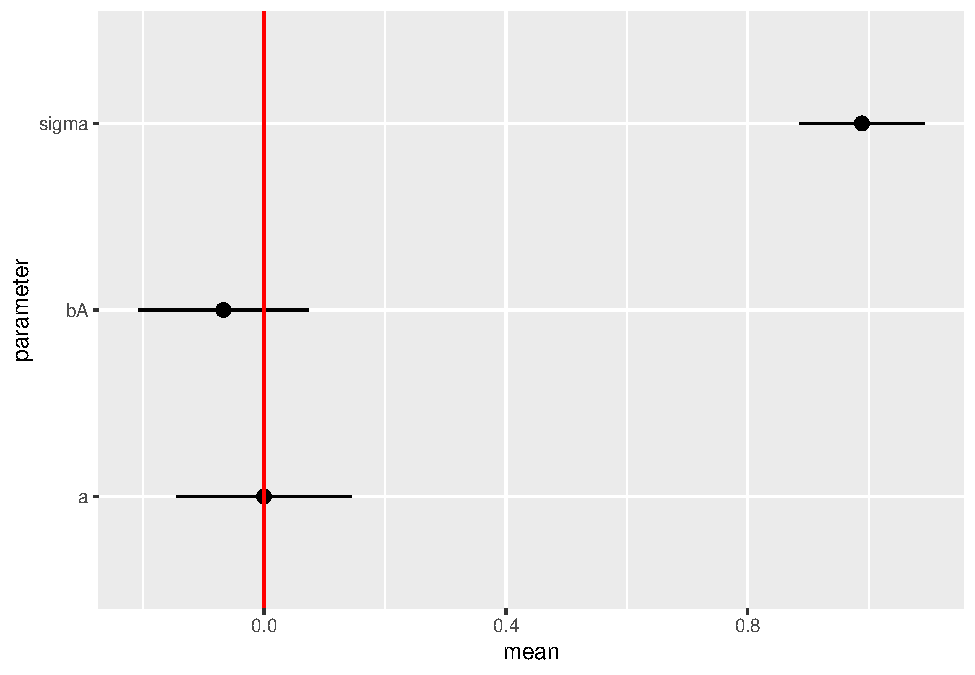
\includegraphics{06-haunted_dag_files/figure-latex/unnamed-chunk-28-2.pdf}

Unexpectedly, the total causal impact of area on weight appears to be zero, or slightly negative. Increasing area would not make foxes heavier.

\hypertarget{h4-2}{%
\subsection*{6H4}\label{h4-2}}
\addcontentsline{toc}{subsection}{6H4}

\hypertarget{question-58}{%
\subsubsection*{Question}\label{question-58}}
\addcontentsline{toc}{subsubsection}{Question}

\begin{quote}
Now infer the causal impact of adding food to a territory. Would this make foxes heavier? Which covariates do you need to adjust for to estimate the total causal influence of food?
\end{quote}

\hypertarget{answer-58}{%
\subsubsection*{Answer}\label{answer-58}}
\addcontentsline{toc}{subsubsection}{Answer}

We don't need to condition on any other parameters assuming the DAG we're given is correct.

\begin{verbatim}
##  {}
\end{verbatim}

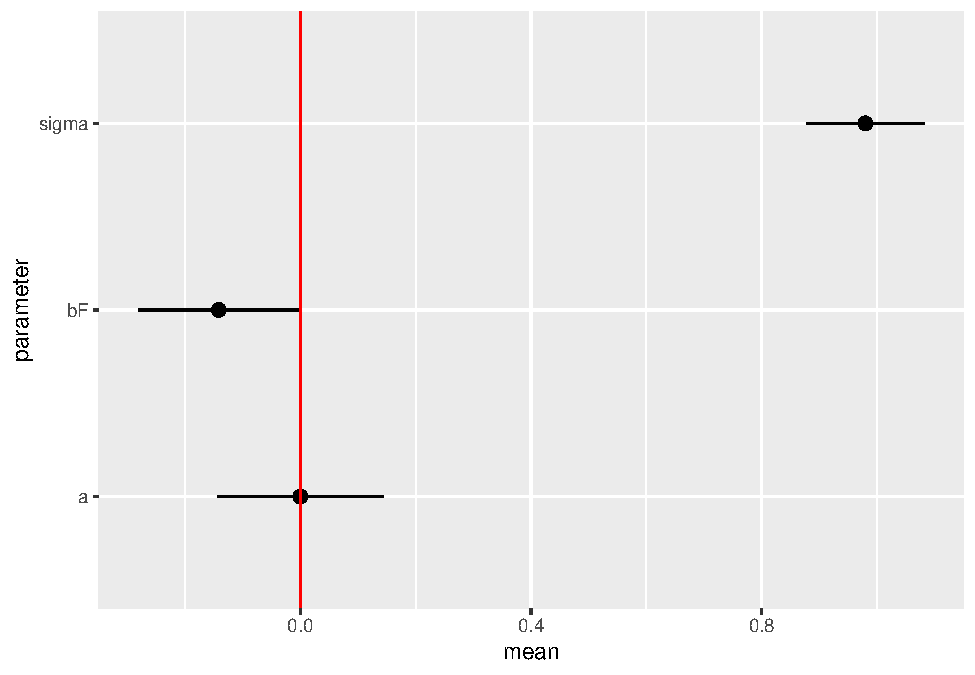
\includegraphics{06-haunted_dag_files/figure-latex/unnamed-chunk-29-1.pdf}

The total causal impact of food on weight again appears to be negative. Increasing food would not make foxes heavier.

\hypertarget{h5-1}{%
\subsection*{6H5}\label{h5-1}}
\addcontentsline{toc}{subsection}{6H5}

\hypertarget{question-59}{%
\subsubsection*{Question}\label{question-59}}
\addcontentsline{toc}{subsubsection}{Question}

\begin{quote}
Now infer the causal impact of group size. Which covariates do you need to adjust for? Looking at the posterior distribution of the resulting model, what do you think explains these data? That is, can you explain the estimates for all three problems? How do they go together?
\end{quote}

\hypertarget{answer-59}{%
\subsubsection*{Answer}\label{answer-59}}
\addcontentsline{toc}{subsubsection}{Answer}

Now we have to condition on food to block the backdoor path.

\begin{verbatim}
## { F }
\end{verbatim}

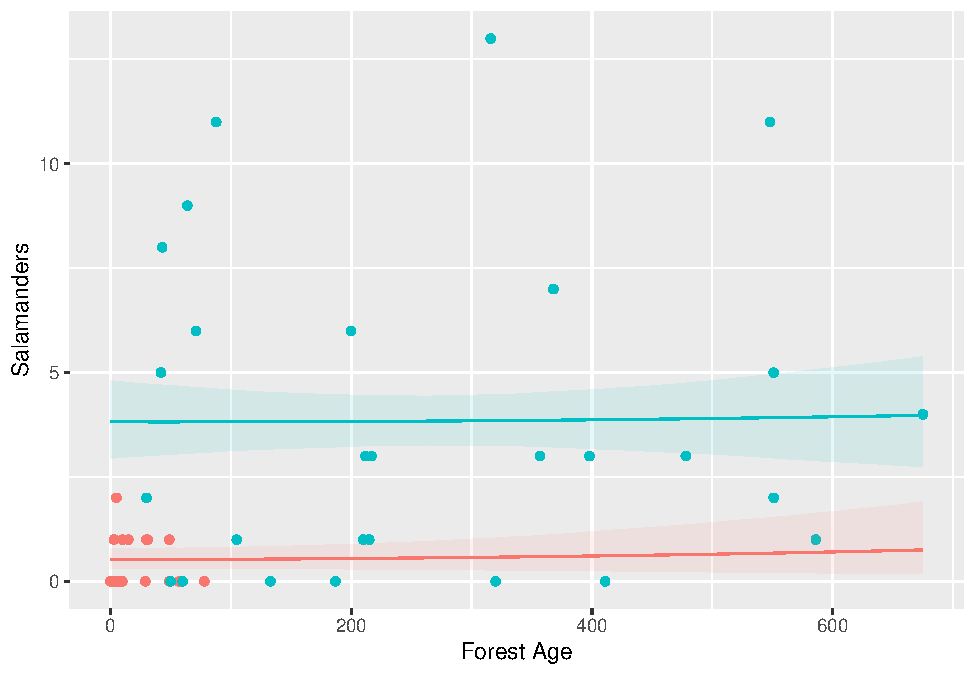
\includegraphics{06-haunted_dag_files/figure-latex/unnamed-chunk-30-1.pdf}

We see that the causal impact of group size is negative, and that the direct effect of food is zero or slightly positive. It is at least not so negative as the total causal effect.

I'd suggest that what's happening here is that the main effect of an increase in food (either directly or by an increase in area) would be to increase group size, which has a detrimental effect on weight. This effect seems to overwhelm any direct effect of increasing food on weight.

\hypertarget{further-reading-5}{%
\section*{Further Reading}\label{further-reading-5}}
\addcontentsline{toc}{section}{Further Reading}

\hypertarget{ulysses}{%
\chapter{Ulysses' Compass}\label{ulysses}}

\hypertarget{chapter-notes-6}{%
\section{Chapter Notes}\label{chapter-notes-6}}

\hypertarget{brain-volume-model}{%
\subsection*{Brain Volume model}\label{brain-volume-model}}
\addcontentsline{toc}{subsection}{Brain Volume model}

We fit the linear brain volume model since it is used to illustrate various concepts later in the chapter:

\begin{Shaded}
\begin{Highlighting}[]
\FunctionTok{set.seed}\NormalTok{(}\DecValTok{100}\NormalTok{)}
\NormalTok{m7}\FloatTok{.1} \OtherTok{\textless{}{-}} \FunctionTok{quap}\NormalTok{( }\FunctionTok{alist}\NormalTok{(}
\NormalTok{  brain\_std }\SpecialCharTok{\textasciitilde{}} \FunctionTok{dnorm}\NormalTok{( mu , }\FunctionTok{exp}\NormalTok{(log\_sigma) ), }
\NormalTok{  mu }\OtherTok{\textless{}{-}}\NormalTok{ a }\SpecialCharTok{+}\NormalTok{ b}\SpecialCharTok{*}\NormalTok{mass\_std, }
\NormalTok{  a }\SpecialCharTok{\textasciitilde{}} \FunctionTok{dnorm}\NormalTok{( }\FloatTok{0.5}\NormalTok{ , }\DecValTok{1}\NormalTok{ ), }
\NormalTok{  b }\SpecialCharTok{\textasciitilde{}} \FunctionTok{dnorm}\NormalTok{( }\DecValTok{0}\NormalTok{ , }\DecValTok{10}\NormalTok{ ), }
\NormalTok{  log\_sigma }\SpecialCharTok{\textasciitilde{}} \FunctionTok{dnorm}\NormalTok{( }\DecValTok{0}\NormalTok{ , }\DecValTok{1}\NormalTok{ )}
\NormalTok{), }\AttributeTok{data=}\NormalTok{brain\_volume )}
\end{Highlighting}
\end{Shaded}

\hypertarget{log-pointwise-predictive-density}{%
\subsection*{Log Pointwise Predictive Density}\label{log-pointwise-predictive-density}}
\addcontentsline{toc}{subsection}{Log Pointwise Predictive Density}

Computing the log pointwise predictive density. With data \(y = \{y_i\}\) and posterior distribution \(\Theta\):

\[
\text{lppd}(y,\Theta) = \sum_i \log \left( \frac{1}{S}\sum_s p(y_i | \theta_s) \right)
\]
Where \(S\) is the number of samples and each \(\theta_s\) is a sample from \(\Theta\).

For an observation say \(y_1\), you calculate the average probability of seeing this observation given the posterior (i.e.~you sum the conditional probabilities of the observation over each posterior sample, and divide by the number of samples). You repeat this process for each observation \(y_i\), take the log of each and sum them all together.

Here is the calculation done in R, from the ``Overthinking: Computing the lppd'' box:

\begin{Shaded}
\begin{Highlighting}[]
\FunctionTok{set.seed}\NormalTok{(}\DecValTok{1}\NormalTok{) }

\CommentTok{\# Using the lppd function built into the Rethinking package}
\NormalTok{lppd1 }\OtherTok{\textless{}{-}} \FunctionTok{lppd}\NormalTok{( m7}\FloatTok{.1}\NormalTok{ , }\AttributeTok{n=}\FloatTok{1e4}\NormalTok{ )}


\CommentTok{\# Extracting posterior samples and calculating manually}

\NormalTok{logprob }\OtherTok{\textless{}{-}} \FunctionTok{sim}\NormalTok{( m7}\FloatTok{.1}\NormalTok{ , }\AttributeTok{ll=}\ConstantTok{TRUE}\NormalTok{ , }\AttributeTok{n=}\FloatTok{1e4}\NormalTok{ )   }\CommentTok{\# logprob contains 10,000 samples from the posterior distribution, each estimating the (log) probability of seeing each}
                                           \CommentTok{\# of the seven observations. }

\NormalTok{n }\OtherTok{\textless{}{-}} \FunctionTok{ncol}\NormalTok{(logprob) }
\NormalTok{ns }\OtherTok{\textless{}{-}} \FunctionTok{nrow}\NormalTok{(logprob) }

\NormalTok{average\_post\_prob }\OtherTok{\textless{}{-}} \ControlFlowTok{function}\NormalTok{( i ) \{}
    \FunctionTok{log\_sum\_exp}\NormalTok{( logprob[,i] ) }\SpecialCharTok{{-}} \FunctionTok{log}\NormalTok{(ns)\}     }\CommentTok{\# this functions sums the log probabilities of the 10,000 samples and divides by the number of rows}
                                              \CommentTok{\# except it is working on a log probability scale.}

\NormalTok{lppd2 }\OtherTok{\textless{}{-}} \FunctionTok{sapply}\NormalTok{( }\DecValTok{1}\SpecialCharTok{:}\NormalTok{n , average\_post\_prob )    }\CommentTok{\# the function is applied to each of the seven observations}

\NormalTok{lppd1}
\end{Highlighting}
\end{Shaded}

\begin{verbatim}
## [1]  0.6099135  0.6484063  0.5496868  0.6235310  0.4648179  0.4347736 -0.8444470
\end{verbatim}

\begin{Shaded}
\begin{Highlighting}[]
\NormalTok{lppd2}
\end{Highlighting}
\end{Shaded}

\begin{verbatim}
## [1]  0.6117253  0.6488831  0.5448708  0.6278331  0.4638980  0.4263233 -0.8522201
\end{verbatim}

Summing over these seven observations will give the total lppd.

\hypertarget{simulating-in-and-out-of-sample-deviance-for-varying-parameter-numbers}{%
\subsection*{Simulating in and out of sample deviance for varying parameter numbers}\label{simulating-in-and-out-of-sample-deviance-for-varying-parameter-numbers}}
\addcontentsline{toc}{subsection}{Simulating in and out of sample deviance for varying parameter numbers}

The idea here is to simulate from the following model with two parameters:

\[\begin{aligned}
y_i & \sim \text{Normal}(\mu_i,1) \\
\mu_i &= (0.15)x_{1,i} - (0.4)x_{2,i}
\end{aligned}\]

To the data produced, we try to fit linear regressions with between 1 and 5 parameters, and compare the in and out of sample deviance for these five models.

\begin{Shaded}
\begin{Highlighting}[]
\NormalTok{N }\OtherTok{\textless{}{-}} \DecValTok{20} 
\NormalTok{kseq }\OtherTok{\textless{}{-}} \DecValTok{1}\SpecialCharTok{:}\DecValTok{5} 

\CommentTok{\# sim\_train\_test simulates Gaussian data with N cases and fits a model with k parameters, returning the in sample and out of sample lppd (can also do WAIC criteria)}

\CommentTok{\# dev contains the mean in sample deviance, mean out of sample deviance, sd of in sample deviance, and sd of out of sample deviance for each model with 1{-}5 parameters.  }

\NormalTok{dev }\OtherTok{\textless{}{-}} \FunctionTok{map\_dfr}\NormalTok{( kseq , }\ControlFlowTok{function}\NormalTok{(k) \{}
\NormalTok{  r }\OtherTok{\textless{}{-}} \FunctionTok{replicate}\NormalTok{( }\DecValTok{100}\NormalTok{ , }\FunctionTok{sim\_train\_test}\NormalTok{( }\AttributeTok{N=}\NormalTok{N, }\AttributeTok{k=}\NormalTok{k , }\AttributeTok{cv.cores =} \DecValTok{4}\NormalTok{)); }
  \FunctionTok{tibble}\NormalTok{(}\AttributeTok{mean\_in =} \FunctionTok{mean}\NormalTok{(r[}\DecValTok{1}\NormalTok{,]) ,}\AttributeTok{mean\_out=} \FunctionTok{mean}\NormalTok{(r[}\DecValTok{2}\NormalTok{,]) ,}\AttributeTok{sd\_in=} \FunctionTok{sd}\NormalTok{(r[}\DecValTok{1}\NormalTok{,]) ,}\AttributeTok{sd\_out=} \FunctionTok{sd}\NormalTok{(r[}\DecValTok{2}\NormalTok{,]) )}
\NormalTok{\} )}

\FunctionTok{ggplot}\NormalTok{(}\AttributeTok{data=}\NormalTok{dev)}\SpecialCharTok{+}
  \FunctionTok{geom\_pointrange}\NormalTok{(}\FunctionTok{aes}\NormalTok{(}\AttributeTok{x=}\DecValTok{1}\SpecialCharTok{:}\DecValTok{5}\NormalTok{,}\AttributeTok{y=}\NormalTok{mean\_in,}\AttributeTok{ymin=}\NormalTok{mean\_in}\SpecialCharTok{{-}}\NormalTok{sd\_in,}\AttributeTok{ymax=}\NormalTok{mean\_in}\SpecialCharTok{+}\NormalTok{sd\_in), }\AttributeTok{colour =} \StringTok{"blue"}\NormalTok{)}\SpecialCharTok{+}
  \FunctionTok{geom\_pointrange}\NormalTok{(}\FunctionTok{aes}\NormalTok{(}\AttributeTok{x=}\FloatTok{1.1}\SpecialCharTok{:}\FloatTok{5.1}\NormalTok{,}\AttributeTok{y=}\NormalTok{mean\_out,}\AttributeTok{ymin=}\NormalTok{mean\_out}\SpecialCharTok{{-}}\NormalTok{sd\_out,}\AttributeTok{ymax=}\NormalTok{mean\_out}\SpecialCharTok{+}\NormalTok{sd\_out))}\SpecialCharTok{+}
  \FunctionTok{geom\_text}\NormalTok{(}\FunctionTok{aes}\NormalTok{(}\AttributeTok{x=}\FloatTok{2.9}\NormalTok{, }\AttributeTok{y =}\NormalTok{ mean\_in[}\DecValTok{3}\NormalTok{], }\AttributeTok{label=}\StringTok{"in"}\NormalTok{),}\AttributeTok{colour=}\StringTok{"blue"}\NormalTok{)}\SpecialCharTok{+}
  \FunctionTok{geom\_text}\NormalTok{(}\FunctionTok{aes}\NormalTok{(}\AttributeTok{x=}\FloatTok{3.2}\NormalTok{, }\AttributeTok{y =}\NormalTok{ mean\_out[}\DecValTok{3}\NormalTok{], }\AttributeTok{label=}\StringTok{"out"}\NormalTok{))}\SpecialCharTok{+}
  \FunctionTok{xlab}\NormalTok{(}\StringTok{"number of parameters"}\NormalTok{)}\SpecialCharTok{+}
  \FunctionTok{ylab}\NormalTok{(}\StringTok{"deviance"}\NormalTok{)}\SpecialCharTok{+}
  \FunctionTok{ggtitle}\NormalTok{(}\StringTok{"N = 20"}\NormalTok{)}
\end{Highlighting}
\end{Shaded}

\includegraphics{07-ulysses_files/figure-latex/unnamed-chunk-5-1.pdf}

Overthinking: WAIC calculations.

The formula for WAIC is:

\[
\text{WAIC}(y,\Theta) = -2 \left( \text{lppd} - \sum_i \text{var}_\theta ( \log p(y_i | \theta)) \right)
\]

where \(\text{var}_\theta\) means taking the variance over the set of posterior samples.

The book calculates it for a simple model:

\begin{Shaded}
\begin{Highlighting}[]
\CommentTok{\# fit a linear model of stopping distance \& speed}

\FunctionTok{data}\NormalTok{(cars) }

\FunctionTok{set.seed}\NormalTok{(}\DecValTok{100}\NormalTok{)}
\NormalTok{m }\OtherTok{\textless{}{-}} \FunctionTok{quap}\NormalTok{( }\FunctionTok{alist}\NormalTok{(}
\NormalTok{dist }\SpecialCharTok{\textasciitilde{}} \FunctionTok{dnorm}\NormalTok{(mu,sigma), }
\NormalTok{mu }\OtherTok{\textless{}{-}}\NormalTok{ a }\SpecialCharTok{+}\NormalTok{ b}\SpecialCharTok{*}\NormalTok{speed, }
\NormalTok{a }\SpecialCharTok{\textasciitilde{}} \FunctionTok{dnorm}\NormalTok{(}\DecValTok{0}\NormalTok{,}\DecValTok{100}\NormalTok{), }
\NormalTok{b }\SpecialCharTok{\textasciitilde{}} \FunctionTok{dnorm}\NormalTok{(}\DecValTok{0}\NormalTok{,}\DecValTok{10}\NormalTok{), }
\NormalTok{sigma }\SpecialCharTok{\textasciitilde{}} \FunctionTok{dexp}\NormalTok{(}\DecValTok{1}\NormalTok{)}
\NormalTok{) , }\AttributeTok{data=}\NormalTok{cars )}

\FunctionTok{set.seed}\NormalTok{(}\DecValTok{94}\NormalTok{)}

\NormalTok{cars\_post }\OtherTok{\textless{}{-}} \FunctionTok{extract.samples}\NormalTok{(m,}\AttributeTok{n=}\DecValTok{1000}\NormalTok{)}

\CommentTok{\# calculate (log) probability of seeing data in cars, assuming it comes from a normal distribution with mean and sd taken from the posterior samples. There are 1000 samples so logprob contains 1000 columns. There are 50 observations in cars so logprob has 50 rows.}

\NormalTok{n\_samples }\OtherTok{\textless{}{-}} \DecValTok{1000} 

\NormalTok{cars\_logprob }\OtherTok{\textless{}{-}} \FunctionTok{sapply}\NormalTok{( }\DecValTok{1}\SpecialCharTok{:}\NormalTok{n\_samples , }\ControlFlowTok{function}\NormalTok{(s) \{ }
\NormalTok{  mu }\OtherTok{\textless{}{-}}\NormalTok{ cars\_post}\SpecialCharTok{$}\NormalTok{a[s] }\SpecialCharTok{+}\NormalTok{ cars\_post}\SpecialCharTok{$}\NormalTok{b[s]}\SpecialCharTok{*}\NormalTok{cars}\SpecialCharTok{$}\NormalTok{speed }
  \FunctionTok{dnorm}\NormalTok{( cars}\SpecialCharTok{$}\NormalTok{dist , mu , cars\_post}\SpecialCharTok{$}\NormalTok{sigma[s] , }\AttributeTok{log=}\ConstantTok{TRUE}\NormalTok{ )}
\NormalTok{\} )}

\CommentTok{\# we take the log of the average probabilities (with a little extra code since we\textquotesingle{}re working with log probabilities)}

\NormalTok{n\_cases }\OtherTok{\textless{}{-}} \FunctionTok{nrow}\NormalTok{(cars) }

\NormalTok{cars\_lppd }\OtherTok{\textless{}{-}} \FunctionTok{sapply}\NormalTok{( }\DecValTok{1}\SpecialCharTok{:}\NormalTok{n\_cases , }\ControlFlowTok{function}\NormalTok{(i) }\FunctionTok{log\_sum\_exp}\NormalTok{(cars\_logprob[i,]) }\SpecialCharTok{{-}} \FunctionTok{log}\NormalTok{(n\_samples) )}

\CommentTok{\# we calculate the penalty term {-} taking the variance for each observation across all 1000 rows}

\NormalTok{cars\_pWAIC }\OtherTok{\textless{}{-}} \FunctionTok{sapply}\NormalTok{( }\DecValTok{1}\SpecialCharTok{:}\NormalTok{n\_cases , }\ControlFlowTok{function}\NormalTok{(i) }\FunctionTok{var}\NormalTok{(cars\_logprob[i,]) )}

\CommentTok{\# we compute WAIC}

\SpecialCharTok{{-}}\DecValTok{2}\SpecialCharTok{*}\NormalTok{( }\FunctionTok{sum}\NormalTok{(cars\_lppd) }\SpecialCharTok{{-}} \FunctionTok{sum}\NormalTok{(cars\_pWAIC) )}
\end{Highlighting}
\end{Shaded}

\begin{verbatim}
## [1] 423.3188
\end{verbatim}

\hypertarget{questions-6}{%
\section{Questions}\label{questions-6}}

\hypertarget{e1-5}{%
\subsection*{7E1}\label{e1-5}}
\addcontentsline{toc}{subsection}{7E1}

\hypertarget{question-60}{%
\subsubsection*{Question}\label{question-60}}
\addcontentsline{toc}{subsubsection}{Question}

\begin{quote}
State the three motivating criteria that define information entropy. Try to express each in your own words.
\end{quote}

\hypertarget{answer-60}{%
\subsubsection*{Answer}\label{answer-60}}
\addcontentsline{toc}{subsubsection}{Answer}

We want our measure of uncertainty to be:

\begin{enumerate}
\def\labelenumi{\arabic{enumi}.}
\tightlist
\item
  Continuous - a small change in the probabilities should lead to a small change in uncertainty.
\item
  Increasing - uncertainty should increase as the number of events increases
\item
  Additive - the uncertainty of two successive events should be the weighted sum of the uncertainties of each event.
\end{enumerate}

\hypertarget{e2-4}{%
\subsection*{7E2}\label{e2-4}}
\addcontentsline{toc}{subsection}{7E2}

\hypertarget{question-61}{%
\subsubsection*{Question}\label{question-61}}
\addcontentsline{toc}{subsubsection}{Question}

\begin{quote}
Suppose a coin is weighted such that, when it is tossed and lands on a table, it comes up heads 70\% of the time. What is the entropy of this coin?
\end{quote}

\hypertarget{answer-61}{%
\subsubsection*{Answer}\label{answer-61}}
\addcontentsline{toc}{subsubsection}{Answer}

Since the textbook uses the natural log, I'll use it too.

\[\begin{aligned}
H(p) &= -\sum^n_{i=1}p_i \log(p_i) \\
&= -(0.7 \log(0.7) + 0.3 \log(0.3))\\
&= 0.6109
\end{aligned}\]

These are the same figures as the `rain or shine' example in the chapter.

\hypertarget{e3-5}{%
\subsection*{7E3}\label{e3-5}}
\addcontentsline{toc}{subsection}{7E3}

\hypertarget{question-62}{%
\subsubsection*{Question}\label{question-62}}
\addcontentsline{toc}{subsubsection}{Question}

\begin{quote}
Suppose a four-sided die is loaded such that, when tossed onto a table, it shows ``1'' 20\%, ``2'' 25\%, ``3'' 25\%, and ``4'' 30\% of the time. What is the entropy of this die?
\end{quote}

\hypertarget{answer-62}{%
\subsubsection*{Answer}\label{answer-62}}
\addcontentsline{toc}{subsubsection}{Answer}

\[\begin{aligned}
H(p) &= -\sum^n_{i=1}p_i \log(p_i) \\
&= -(0.2 \log(0.2) + 0.25 \log(0.25) + 0.25 \log(0.25) + 0.3 \log(0.3))\\
&= 1.3762
\end{aligned}\]

\hypertarget{e4-5}{%
\subsection*{7E4}\label{e4-5}}
\addcontentsline{toc}{subsection}{7E4}

\hypertarget{question-63}{%
\subsubsection*{Question}\label{question-63}}
\addcontentsline{toc}{subsubsection}{Question}

\begin{quote}
Suppose another four-sided die is loaded such that it never shows ``4''. The other three sides show equally often. What is the entropy of this die?
\end{quote}

\hypertarget{answer-63}{%
\subsubsection*{Answer}\label{answer-63}}
\addcontentsline{toc}{subsubsection}{Answer}

\[\begin{aligned}
H(p) &= -\sum^n_{i=1}p_i \ \log(p_i) \\
&= -(\frac{1}{3}  \log(\frac{1}{3}) + \frac{1}{3}  \log(\frac{1}{3}) + \frac{1}{3}  \log(\frac{1}{3}) + 0  \log(0))\\
&= -\log(\frac{1}{3}) &&\text{using the convention that } 0  \log(0) = 0 \\
&= 1.0986
\end{aligned}\]

\hypertarget{m1-4}{%
\subsection*{7M1}\label{m1-4}}
\addcontentsline{toc}{subsection}{7M1}

\hypertarget{question-64}{%
\subsubsection*{Question}\label{question-64}}
\addcontentsline{toc}{subsubsection}{Question}

\begin{quote}
Write down and compare the definitions of AIC and WAIC. Which of these criteria is most general? Which assumptions are required to transform the more general criterion into a less general one?
\end{quote}

\hypertarget{answer-64}{%
\subsubsection*{Answer}\label{answer-64}}
\addcontentsline{toc}{subsubsection}{Answer}

\emph{AIC}

\[
\text{AIC}(y,\Theta) = -2 \text{lppd} + 2p
\]

\emph{WAIC}

\[
\text{WAIC}(y,\Theta) = -2 \left( \text{lppd} - \sum_i \text{var}_\theta ( \log p(y_i | \theta)) \right)
\]

WAIC is more general, since the adjustment term \(\sum_i \text{var}_\theta ( \log p(y_i | \theta))\) is approximately equal to the number of parameters when the following constraints are in place:

\begin{itemize}
\tightlist
\item
  the posterior is Gaussian
\item
  there is a large sample size
\item
  the prior is uninformative (or overwhelmed by the data)
\end{itemize}

\hypertarget{m2-4}{%
\subsection*{7M2}\label{m2-4}}
\addcontentsline{toc}{subsection}{7M2}

\hypertarget{question-65}{%
\subsubsection*{Question}\label{question-65}}
\addcontentsline{toc}{subsubsection}{Question}

\begin{quote}
Explain the difference between model selection and model comparison. What information is lost under model selection?
\end{quote}

\hypertarget{answer-65}{%
\subsubsection*{Answer}\label{answer-65}}
\addcontentsline{toc}{subsubsection}{Answer}

Model selection here involves comparing candidate models using a some criterion (say WAIC), choosing the model with the lowest WAIC, and discarding the rest.

This approach involves throwing away information about the relative differences between models, which can give hints about how confident we should be about our models.

\hypertarget{m3-4}{%
\subsection*{7M3}\label{m3-4}}
\addcontentsline{toc}{subsection}{7M3}

\hypertarget{question-66}{%
\subsubsection*{Question}\label{question-66}}
\addcontentsline{toc}{subsubsection}{Question}

\begin{quote}
When comparing models with an information criterion, why must all models be fit to exactly the same observations? What would happen to the information criterion values, if the models were fit to different numbers of observations? Perform some experiments, if you are not sure.
\end{quote}

\hypertarget{answer-66}{%
\subsubsection*{Answer}\label{answer-66}}
\addcontentsline{toc}{subsubsection}{Answer}

We should be able to answer this question by inspecting the formula for lppd:

\[
\text{lppd}(y,\Theta) = \sum_i \log \left( \frac{1}{S}\sum_s p(y_i | \theta_s) \right)
\]

Changing the observations means changing the \(y_i\)'s and therefore the calculation of the average probability of the observations given the data \(\frac{1}{S}\sum_s p(y_i | \theta_s)\). Using a different set of observations for different models will make the resulting information criterion values uninterpretable.

An easy way to see this is to consider that changing observations will lead to different information criterion values even with the \emph{same} model.

\hypertarget{m4-3}{%
\subsection*{7M4}\label{m4-3}}
\addcontentsline{toc}{subsection}{7M4}

\hypertarget{question-67}{%
\subsubsection*{Question}\label{question-67}}
\addcontentsline{toc}{subsubsection}{Question}

\begin{quote}
What happens to the effective number of parameters, as measured by PSIS or WAIC, as a prior becomes more concentrated? Why? Perform some experiments, if you are not sure.
\end{quote}

\hypertarget{answer-67}{%
\subsubsection*{Answer}\label{answer-67}}
\addcontentsline{toc}{subsubsection}{Answer}

Before performing any experiments, I'll take a guess by looking at the definition of effective number of parameters for WAIC:

\[ \sum_i \text{var}_\theta ( \log p(y_i | \theta))\]

I'd expect the variance of the log probabilities here to decrease, since informative priors give a model more concentrated expectations for the data, i.e.~they lead to unusual values of \(y\) being assigned less probability.

So I expect that making priors more narrowly peaked decreases the effective number of parameters.

I'll pick up the cars data set from earlier and fit a couple of models with increasingly concentrated priors.

\begin{Shaded}
\begin{Highlighting}[]
\CommentTok{\# previous model}

\CommentTok{\# m \textless{}{-} quap( alist(}
\CommentTok{\# dist \textasciitilde{} dnorm(mu,sigma), }
\CommentTok{\# mu \textless{}{-} a + b*speed, }
\CommentTok{\# a \textasciitilde{} dnorm(0,100), }
\CommentTok{\# b \textasciitilde{} dnorm(0,10), }
\CommentTok{\# sigma \textasciitilde{} dexp(1)}
\CommentTok{\# ) , data=cars )}

\NormalTok{cars\_prior\_sim\_1 }\OtherTok{\textless{}{-}} \FunctionTok{tibble}\NormalTok{(}\AttributeTok{a=}\FunctionTok{rnorm}\NormalTok{(}\DecValTok{100}\NormalTok{,}\DecValTok{0}\NormalTok{,}\DecValTok{100}\NormalTok{),}\AttributeTok{b=}\FunctionTok{rnorm}\NormalTok{(}\DecValTok{100}\NormalTok{,}\DecValTok{0}\NormalTok{,}\DecValTok{10}\NormalTok{),}\AttributeTok{mu=}\NormalTok{a}\SpecialCharTok{+}\NormalTok{b)}

\FunctionTok{ggplot}\NormalTok{()}\SpecialCharTok{+}
  \FunctionTok{geom\_abline}\NormalTok{(}\AttributeTok{data=}\NormalTok{cars\_prior\_sim\_1, }\AttributeTok{mapping=}\FunctionTok{aes}\NormalTok{(}\AttributeTok{slope=}\NormalTok{b,}\AttributeTok{intercept=}\NormalTok{a))}\SpecialCharTok{+}
  \FunctionTok{geom\_hline}\NormalTok{(}\AttributeTok{yintercept =} \FloatTok{1.2}\SpecialCharTok{*}\FunctionTok{max}\NormalTok{(cars}\SpecialCharTok{$}\NormalTok{dist) ,}\AttributeTok{colour=}\StringTok{"red"}\NormalTok{)}\SpecialCharTok{+}
  \FunctionTok{geom\_hline}\NormalTok{(}\AttributeTok{yintercept =} \FloatTok{0.8}\SpecialCharTok{*}\FunctionTok{min}\NormalTok{(cars}\SpecialCharTok{$}\NormalTok{dist),}\AttributeTok{colour=}\StringTok{"red"}\NormalTok{)}\SpecialCharTok{+}
  \FunctionTok{xlim}\NormalTok{(}\FunctionTok{min}\NormalTok{(cars}\SpecialCharTok{$}\NormalTok{speed),}\FunctionTok{max}\NormalTok{(cars}\SpecialCharTok{$}\NormalTok{speed))}
\end{Highlighting}
\end{Shaded}

\includegraphics{07-ulysses_files/figure-latex/unnamed-chunk-7-1.pdf}
These priors are very flat. Let's make them more concentrated.

Logically, the intercept a should be near zero since if you're going zero mph it should take you zero feet to stop.

Also we'd expect b to be positive - the faster you go the further it takes you to stop.

\begin{Shaded}
\begin{Highlighting}[]
\NormalTok{cars\_prior\_sim\_2 }\OtherTok{\textless{}{-}} \FunctionTok{tibble}\NormalTok{(}\AttributeTok{a=}\FunctionTok{rnorm}\NormalTok{(}\DecValTok{100}\NormalTok{,}\DecValTok{0}\NormalTok{,}\DecValTok{5}\NormalTok{),}\AttributeTok{b=}\FunctionTok{rnorm}\NormalTok{(}\DecValTok{100}\NormalTok{,}\DecValTok{5}\NormalTok{,}\FloatTok{2.5}\NormalTok{),}\AttributeTok{mu=}\NormalTok{a}\SpecialCharTok{+}\NormalTok{b)}

\FunctionTok{ggplot}\NormalTok{()}\SpecialCharTok{+}
  \FunctionTok{geom\_abline}\NormalTok{(}\AttributeTok{data=}\NormalTok{cars\_prior\_sim\_2, }\AttributeTok{mapping=}\FunctionTok{aes}\NormalTok{(}\AttributeTok{slope=}\NormalTok{b,}\AttributeTok{intercept=}\NormalTok{a))}\SpecialCharTok{+}
  \FunctionTok{geom\_hline}\NormalTok{(}\AttributeTok{yintercept =} \FloatTok{1.2}\SpecialCharTok{*}\FunctionTok{max}\NormalTok{(cars}\SpecialCharTok{$}\NormalTok{dist) ,}\AttributeTok{colour=}\StringTok{"red"}\NormalTok{)}\SpecialCharTok{+}
  \FunctionTok{geom\_hline}\NormalTok{(}\AttributeTok{yintercept =} \FloatTok{0.8}\SpecialCharTok{*}\FunctionTok{min}\NormalTok{(cars}\SpecialCharTok{$}\NormalTok{dist),}\AttributeTok{colour=}\StringTok{"red"}\NormalTok{)}\SpecialCharTok{+}
  \FunctionTok{xlim}\NormalTok{(}\FunctionTok{min}\NormalTok{(cars}\SpecialCharTok{$}\NormalTok{speed),}\FunctionTok{max}\NormalTok{(cars}\SpecialCharTok{$}\NormalTok{speed))}
\end{Highlighting}
\end{Shaded}

\includegraphics{07-ulysses_files/figure-latex/unnamed-chunk-8-1.pdf}

I think this is reasonable for our purposes.

Now let's make the prior very concentrated.

\begin{Shaded}
\begin{Highlighting}[]
\NormalTok{cars\_prior\_sim\_3 }\OtherTok{\textless{}{-}} \FunctionTok{tibble}\NormalTok{(}\AttributeTok{a=}\FunctionTok{rnorm}\NormalTok{(}\DecValTok{100}\NormalTok{,}\DecValTok{0}\NormalTok{,}\FloatTok{0.5}\NormalTok{),}\AttributeTok{b=}\FunctionTok{rnorm}\NormalTok{(}\DecValTok{100}\NormalTok{,}\DecValTok{5}\NormalTok{,}\FloatTok{0.5}\NormalTok{),}\AttributeTok{mu=}\NormalTok{a}\SpecialCharTok{+}\NormalTok{b)}

\FunctionTok{ggplot}\NormalTok{()}\SpecialCharTok{+}
  \FunctionTok{geom\_abline}\NormalTok{(}\AttributeTok{data=}\NormalTok{cars\_prior\_sim\_3, }\AttributeTok{mapping=}\FunctionTok{aes}\NormalTok{(}\AttributeTok{slope=}\NormalTok{b,}\AttributeTok{intercept=}\NormalTok{a))}\SpecialCharTok{+}
  \FunctionTok{geom\_hline}\NormalTok{(}\AttributeTok{yintercept =} \FloatTok{1.2}\SpecialCharTok{*}\FunctionTok{max}\NormalTok{(cars}\SpecialCharTok{$}\NormalTok{dist) ,}\AttributeTok{colour=}\StringTok{"red"}\NormalTok{)}\SpecialCharTok{+}
  \FunctionTok{geom\_hline}\NormalTok{(}\AttributeTok{yintercept =} \FloatTok{0.8}\SpecialCharTok{*}\FunctionTok{min}\NormalTok{(cars}\SpecialCharTok{$}\NormalTok{dist),}\AttributeTok{colour=}\StringTok{"red"}\NormalTok{)}\SpecialCharTok{+}
  \FunctionTok{xlim}\NormalTok{(}\FunctionTok{min}\NormalTok{(cars}\SpecialCharTok{$}\NormalTok{speed),}\FunctionTok{max}\NormalTok{(cars}\SpecialCharTok{$}\NormalTok{speed))}
\end{Highlighting}
\end{Shaded}

\includegraphics{07-ulysses_files/figure-latex/unnamed-chunk-9-1.pdf}

Now we fit two new models with our new priors and calculate the effective number of parameters.

\begin{Shaded}
\begin{Highlighting}[]
\FunctionTok{set.seed}\NormalTok{(}\DecValTok{100}\NormalTok{)}
\NormalTok{ m\_moderate }\OtherTok{\textless{}{-}} \FunctionTok{quap}\NormalTok{( }\FunctionTok{alist}\NormalTok{(}
\NormalTok{ dist }\SpecialCharTok{\textasciitilde{}} \FunctionTok{dnorm}\NormalTok{(mu,sigma), }
\NormalTok{ mu }\OtherTok{\textless{}{-}}\NormalTok{ a }\SpecialCharTok{+}\NormalTok{ b}\SpecialCharTok{*}\NormalTok{speed, }
\NormalTok{ a }\SpecialCharTok{\textasciitilde{}} \FunctionTok{dnorm}\NormalTok{(}\DecValTok{0}\NormalTok{,}\DecValTok{5}\NormalTok{), }
\NormalTok{ b }\SpecialCharTok{\textasciitilde{}} \FunctionTok{dnorm}\NormalTok{(}\DecValTok{5}\NormalTok{,}\FloatTok{2.5}\NormalTok{), }
\NormalTok{ sigma }\SpecialCharTok{\textasciitilde{}} \FunctionTok{dexp}\NormalTok{(}\DecValTok{1}\NormalTok{)}
\NormalTok{ ) , }\AttributeTok{data=}\NormalTok{cars )}

 \FunctionTok{set.seed}\NormalTok{(}\DecValTok{100}\NormalTok{)}
\NormalTok{ m\_concentrated }\OtherTok{\textless{}{-}} \FunctionTok{quap}\NormalTok{( }\FunctionTok{alist}\NormalTok{(}
\NormalTok{ dist }\SpecialCharTok{\textasciitilde{}} \FunctionTok{dnorm}\NormalTok{(mu,sigma), }
\NormalTok{ mu }\OtherTok{\textless{}{-}}\NormalTok{ a }\SpecialCharTok{+}\NormalTok{ b}\SpecialCharTok{*}\NormalTok{speed, }
\NormalTok{ a }\SpecialCharTok{\textasciitilde{}} \FunctionTok{dnorm}\NormalTok{(}\DecValTok{0}\NormalTok{,}\FloatTok{0.5}\NormalTok{), }
\NormalTok{ b }\SpecialCharTok{\textasciitilde{}} \FunctionTok{dnorm}\NormalTok{(}\DecValTok{5}\NormalTok{,}\FloatTok{0.5}\NormalTok{), }
\NormalTok{ sigma }\SpecialCharTok{\textasciitilde{}} \FunctionTok{dexp}\NormalTok{(}\DecValTok{1}\NormalTok{)}
\NormalTok{ ) , }\AttributeTok{data=}\NormalTok{cars )}
 

\NormalTok{moderate\_post }\OtherTok{\textless{}{-}} \FunctionTok{extract.samples}\NormalTok{(m\_moderate,}\AttributeTok{n=}\DecValTok{1000}\NormalTok{)}
\NormalTok{concentrated\_post }\OtherTok{\textless{}{-}} \FunctionTok{extract.samples}\NormalTok{(m\_concentrated,}\AttributeTok{n=}\DecValTok{1000}\NormalTok{)}

\NormalTok{n\_samples }\OtherTok{\textless{}{-}} \DecValTok{1000} 

\NormalTok{moderate\_logprob }\OtherTok{\textless{}{-}} \FunctionTok{sapply}\NormalTok{( }\DecValTok{1}\SpecialCharTok{:}\NormalTok{n\_samples , }\ControlFlowTok{function}\NormalTok{(s) \{ }
\NormalTok{  mu }\OtherTok{\textless{}{-}}\NormalTok{ moderate\_post}\SpecialCharTok{$}\NormalTok{a[s] }\SpecialCharTok{+}\NormalTok{ moderate\_post}\SpecialCharTok{$}\NormalTok{b[s]}\SpecialCharTok{*}\NormalTok{cars}\SpecialCharTok{$}\NormalTok{speed }
  \FunctionTok{dnorm}\NormalTok{( cars}\SpecialCharTok{$}\NormalTok{dist , mu , moderate\_post}\SpecialCharTok{$}\NormalTok{sigma[s] , }\AttributeTok{log=}\ConstantTok{TRUE}\NormalTok{ )}
\NormalTok{\} )}

\NormalTok{concentrated\_logprob }\OtherTok{\textless{}{-}} \FunctionTok{sapply}\NormalTok{( }\DecValTok{1}\SpecialCharTok{:}\NormalTok{n\_samples , }\ControlFlowTok{function}\NormalTok{(s) \{ }
\NormalTok{  mu }\OtherTok{\textless{}{-}}\NormalTok{ concentrated\_post}\SpecialCharTok{$}\NormalTok{a[s] }\SpecialCharTok{+}\NormalTok{ concentrated\_post}\SpecialCharTok{$}\NormalTok{b[s]}\SpecialCharTok{*}\NormalTok{cars}\SpecialCharTok{$}\NormalTok{speed }
  \FunctionTok{dnorm}\NormalTok{( cars}\SpecialCharTok{$}\NormalTok{dist , mu , concentrated\_post}\SpecialCharTok{$}\NormalTok{sigma[s] , }\AttributeTok{log=}\ConstantTok{TRUE}\NormalTok{ )}
\NormalTok{\} )}

\NormalTok{n\_cases }\OtherTok{\textless{}{-}} \FunctionTok{nrow}\NormalTok{(cars) }

\NormalTok{moderate\_pWAIC }\OtherTok{\textless{}{-}} \FunctionTok{sapply}\NormalTok{( }\DecValTok{1}\SpecialCharTok{:}\NormalTok{n\_cases , }\ControlFlowTok{function}\NormalTok{(i) }\FunctionTok{var}\NormalTok{(moderate\_logprob[i,]) )}

\NormalTok{concentrated\_pWAIC }\OtherTok{\textless{}{-}} \FunctionTok{sapply}\NormalTok{( }\DecValTok{1}\SpecialCharTok{:}\NormalTok{n\_cases , }\ControlFlowTok{function}\NormalTok{(i) }\FunctionTok{var}\NormalTok{(concentrated\_logprob[i,]) )}

\FunctionTok{sum}\NormalTok{(cars\_pWAIC)}
\end{Highlighting}
\end{Shaded}

\begin{verbatim}
## [1] 4.780675
\end{verbatim}

\begin{Shaded}
\begin{Highlighting}[]
\FunctionTok{sum}\NormalTok{(moderate\_pWAIC)}
\end{Highlighting}
\end{Shaded}

\begin{verbatim}
## [1] 3.732736
\end{verbatim}

\begin{Shaded}
\begin{Highlighting}[]
\FunctionTok{sum}\NormalTok{(concentrated\_pWAIC)}
\end{Highlighting}
\end{Shaded}

\begin{verbatim}
## [1] 3.662483
\end{verbatim}

\begin{Shaded}
\begin{Highlighting}[]
\CommentTok{\#compare(m,m\_moderate,m\_concentrated, func = PSIS)}
\end{Highlighting}
\end{Shaded}

As expected, the effective number of parameters (in the WAIC calculation) decreases as the prior becomes more concentrated.

Running the commented-out compare function shows the same for PSIS.

\hypertarget{m5-3}{%
\subsection*{7M5}\label{m5-3}}
\addcontentsline{toc}{subsection}{7M5}

\hypertarget{question-68}{%
\subsubsection*{Question}\label{question-68}}
\addcontentsline{toc}{subsubsection}{Question}

\begin{quote}
Provide an informal explanation of why informative priors reduce overfitting.
\end{quote}

\hypertarget{answer-68}{%
\subsubsection*{Answer}\label{answer-68}}
\addcontentsline{toc}{subsubsection}{Answer}

Informative priors make a model more sceptical of the data, since the model has narrower expectations of plausible parameter values before it even sees the data.

Overfitting occurs when a model is too wedded to the particular data set it is trained on. It encodes features of this data set that are unlikely to be present in future data,

Because of their scepticism, informative priors reduce the risk of overfitting. The aim is that only regular features - those that you might expect to occur in a future data set - will be encoded into the model.

\hypertarget{m6-3}{%
\subsection*{7M6}\label{m6-3}}
\addcontentsline{toc}{subsection}{7M6}

\hypertarget{question-69}{%
\subsubsection*{Question}\label{question-69}}
\addcontentsline{toc}{subsubsection}{Question}

\begin{quote}
Provide an informal explanation of why overly informative priors result in underfitting.
\end{quote}

\hypertarget{answer-69}{%
\subsubsection*{Answer}\label{answer-69}}
\addcontentsline{toc}{subsubsection}{Answer}

If the priors make the model too sceptical of the data, it will fail to capture some of the regular features of the data. The model would do a better job of predicting future data if it were allowed to learn more from the training data.

\hypertarget{h1-3}{%
\subsection*{7H1}\label{h1-3}}
\addcontentsline{toc}{subsection}{7H1}

\hypertarget{question-70}{%
\subsubsection*{Question}\label{question-70}}
\addcontentsline{toc}{subsubsection}{Question}

\begin{quote}
In 2007, The Wall Street Journal published an editorial (``We're Number One, Alas'') with a graph of corporate tax rates in 29 countries plotted against tax revenue. A badly fit curve was drawn in, seemingly by hand, to make the argument that the relationship between tax rate and tax revenue increases and then declines, such that higher tax rates can actually produce less tax revenue.

I want you to actually fit a curve to these data, found in data(Laffer). Consider models that use tax rate to predict tax revenue. Compare, using WAIC or PSIS, a straight-line model to any curved models you like. What do you conclude about the relationship between tax rate and tax revenue?
\end{quote}

\hypertarget{answer-70}{%
\subsubsection*{Answer}\label{answer-70}}
\addcontentsline{toc}{subsubsection}{Answer}

\begin{Shaded}
\begin{Highlighting}[]
\FunctionTok{data}\NormalTok{(Laffer)}

\CommentTok{\#laffer\_prior1 \textless{}{-} tibble(a=rnorm(100,1,0.5),b=rnorm(100,0.3,0.2),mu=a+b)}

\CommentTok{\#ggplot()+}
\CommentTok{\#  geom\_abline(data=laffer\_prior1, mapping=aes(slope=b,intercept=a))+}
\CommentTok{\#  geom\_hline(yintercept = 1.2*max(Laffer$tax\_revenue) ,colour="red")+}
\CommentTok{\#  geom\_hline(yintercept = 0.8*min(Laffer$tax\_revenue),colour="red")+}
\CommentTok{\#  xlim(min(Laffer$tax\_rate),max(Laffer$tax\_rate))}

\FunctionTok{set.seed}\NormalTok{(}\DecValTok{100}\NormalTok{)}
\NormalTok{ m\_laffer1 }\OtherTok{\textless{}{-}} \FunctionTok{quap}\NormalTok{( }\FunctionTok{alist}\NormalTok{(}
\NormalTok{ tax\_revenue }\SpecialCharTok{\textasciitilde{}} \FunctionTok{dnorm}\NormalTok{(mu,sigma), }
\NormalTok{ mu }\OtherTok{\textless{}{-}}\NormalTok{ a }\SpecialCharTok{+}\NormalTok{ b}\SpecialCharTok{*}\NormalTok{tax\_rate, }
\NormalTok{ a }\SpecialCharTok{\textasciitilde{}} \FunctionTok{dnorm}\NormalTok{(}\DecValTok{1}\NormalTok{,}\FloatTok{0.5}\NormalTok{), }
\NormalTok{ b }\SpecialCharTok{\textasciitilde{}} \FunctionTok{dnorm}\NormalTok{(}\FloatTok{0.3}\NormalTok{,}\FloatTok{0.2}\NormalTok{), }
\NormalTok{ sigma }\SpecialCharTok{\textasciitilde{}} \FunctionTok{dexp}\NormalTok{(}\DecValTok{1}\NormalTok{)}
\NormalTok{ ) , }\AttributeTok{data=}\NormalTok{Laffer )}
 
\NormalTok{ laffer1\_post }\OtherTok{\textless{}{-}} \FunctionTok{extract.samples}\NormalTok{(m\_laffer1)}

\CommentTok{\#laffer\_prior2 \textless{}{-} tibble(a=rnorm(100,1,0.5),b=rnorm(100,0.01,1),c=rnorm(100,0.01,1))}

\CommentTok{\#ggplot()+}
\CommentTok{\#  purrr::map(1:nrow(laffer\_prior2), \textasciitilde{}geom\_function(fun = function(x) laffer\_prior2$a[.x] + laffer\_prior2$b[.x] * x + laffer\_prior2$c[.x] * x\^{}2 ))+}
\CommentTok{\#  geom\_hline(yintercept = 1.2*max(Laffer$tax\_revenue) ,colour="red")+}
\CommentTok{\#  geom\_hline(yintercept = 0.8*min(Laffer$tax\_revenue),colour="red")+}
\CommentTok{\#  xlim(min(Laffer$tax\_rate),max(Laffer$tax\_rate))}
 
 \FunctionTok{set.seed}\NormalTok{(}\DecValTok{100}\NormalTok{)}
\NormalTok{ m\_laffer2 }\OtherTok{\textless{}{-}} \FunctionTok{quap}\NormalTok{( }\FunctionTok{alist}\NormalTok{(}
\NormalTok{ tax\_revenue }\SpecialCharTok{\textasciitilde{}} \FunctionTok{dnorm}\NormalTok{(mu,sigma), }
\NormalTok{ mu }\OtherTok{\textless{}{-}}\NormalTok{ a }\SpecialCharTok{+}\NormalTok{ b}\SpecialCharTok{*}\NormalTok{tax\_rate }\SpecialCharTok{+}\NormalTok{c}\SpecialCharTok{*}\NormalTok{tax\_rate}\SpecialCharTok{\^{}}\DecValTok{2}\NormalTok{, }
\NormalTok{ a }\SpecialCharTok{\textasciitilde{}} \FunctionTok{dnorm}\NormalTok{(}\DecValTok{1}\NormalTok{,}\FloatTok{0.5}\NormalTok{), }
\NormalTok{ b }\SpecialCharTok{\textasciitilde{}} \FunctionTok{dnorm}\NormalTok{(}\FloatTok{0.1}\NormalTok{,}\DecValTok{1}\NormalTok{), }
\NormalTok{ c }\SpecialCharTok{\textasciitilde{}} \FunctionTok{dnorm}\NormalTok{(}\FloatTok{0.1}\NormalTok{,}\DecValTok{1}\NormalTok{),}
\NormalTok{ sigma }\SpecialCharTok{\textasciitilde{}} \FunctionTok{dexp}\NormalTok{(}\DecValTok{1}\NormalTok{)}
\NormalTok{ ) , }\AttributeTok{data=}\NormalTok{Laffer )}
 
\NormalTok{ laffer2\_post }\OtherTok{\textless{}{-}} \FunctionTok{extract.samples}\NormalTok{(m\_laffer2)}
 
\NormalTok{ laffer2\_mean }\OtherTok{\textless{}{-}} \FunctionTok{tibble}\NormalTok{(}\AttributeTok{a=}\FunctionTok{mean}\NormalTok{(laffer2\_post}\SpecialCharTok{$}\NormalTok{a),}\AttributeTok{b=}\FunctionTok{mean}\NormalTok{(laffer2\_post}\SpecialCharTok{$}\NormalTok{b),}\AttributeTok{c=}\FunctionTok{mean}\NormalTok{(laffer2\_post}\SpecialCharTok{$}\NormalTok{c),}\AttributeTok{d=}\FunctionTok{mean}\NormalTok{(laffer2\_post}\SpecialCharTok{$}\NormalTok{d))}
 
\FunctionTok{set.seed}\NormalTok{(}\DecValTok{101}\NormalTok{)}
\NormalTok{ m\_laffer3 }\OtherTok{\textless{}{-}} \FunctionTok{quap}\NormalTok{( }\FunctionTok{alist}\NormalTok{(}
\NormalTok{ tax\_revenue }\SpecialCharTok{\textasciitilde{}} \FunctionTok{dnorm}\NormalTok{(mu,sigma), }
\NormalTok{ mu }\OtherTok{\textless{}{-}}\NormalTok{ a }\SpecialCharTok{+}\NormalTok{ b}\SpecialCharTok{*}\NormalTok{tax\_rate }\SpecialCharTok{+}\NormalTok{c}\SpecialCharTok{*}\NormalTok{tax\_rate}\SpecialCharTok{\^{}}\DecValTok{2} \SpecialCharTok{+}\NormalTok{d}\SpecialCharTok{*}\NormalTok{tax\_rate}\SpecialCharTok{\^{}}\DecValTok{3}\NormalTok{, }
\NormalTok{ a }\SpecialCharTok{\textasciitilde{}} \FunctionTok{dnorm}\NormalTok{(}\DecValTok{1}\NormalTok{,}\FloatTok{0.5}\NormalTok{), }
\NormalTok{ b }\SpecialCharTok{\textasciitilde{}} \FunctionTok{dnorm}\NormalTok{(}\FloatTok{0.1}\NormalTok{,}\DecValTok{1}\NormalTok{), }
\NormalTok{ c }\SpecialCharTok{\textasciitilde{}} \FunctionTok{dnorm}\NormalTok{(}\FloatTok{0.1}\NormalTok{,}\DecValTok{1}\NormalTok{),}
\NormalTok{ d }\SpecialCharTok{\textasciitilde{}} \FunctionTok{dnorm}\NormalTok{(}\FloatTok{0.1}\NormalTok{,}\DecValTok{1}\NormalTok{),}
\NormalTok{ sigma }\SpecialCharTok{\textasciitilde{}} \FunctionTok{dexp}\NormalTok{(}\DecValTok{1}\NormalTok{)}
\NormalTok{ ) , }\AttributeTok{data=}\NormalTok{Laffer )}
 
\NormalTok{ laffer3\_post }\OtherTok{\textless{}{-}} \FunctionTok{extract.samples}\NormalTok{(m\_laffer3)}
 
\NormalTok{ laffer3\_mean }\OtherTok{\textless{}{-}} \FunctionTok{tibble}\NormalTok{(}\AttributeTok{a=}\FunctionTok{mean}\NormalTok{(laffer3\_post}\SpecialCharTok{$}\NormalTok{a),}\AttributeTok{b=}\FunctionTok{mean}\NormalTok{(laffer3\_post}\SpecialCharTok{$}\NormalTok{b),}\AttributeTok{c=}\FunctionTok{mean}\NormalTok{(laffer3\_post}\SpecialCharTok{$}\NormalTok{c),}\AttributeTok{d=}\FunctionTok{mean}\NormalTok{(laffer3\_post}\SpecialCharTok{$}\NormalTok{d))}
 
\FunctionTok{ggplot}\NormalTok{()}\SpecialCharTok{+}
  \FunctionTok{geom\_point}\NormalTok{(}\AttributeTok{data=}\NormalTok{Laffer, }\AttributeTok{mapping=}\FunctionTok{aes}\NormalTok{(tax\_rate,tax\_revenue))}\SpecialCharTok{+}
  \FunctionTok{geom\_abline}\NormalTok{(}\AttributeTok{data=}\NormalTok{laffer1\_post, }\AttributeTok{mapping=}\FunctionTok{aes}\NormalTok{(}\AttributeTok{slope=}\FunctionTok{mean}\NormalTok{(b),}\AttributeTok{intercept=}\FunctionTok{mean}\NormalTok{(a)),}\AttributeTok{colour=}\StringTok{"red"}\NormalTok{)}\SpecialCharTok{+}
  \FunctionTok{geom\_function}\NormalTok{(}\AttributeTok{fun =} \ControlFlowTok{function}\NormalTok{(x) laffer2\_mean}\SpecialCharTok{$}\NormalTok{a }\SpecialCharTok{+}\NormalTok{ laffer2\_mean}\SpecialCharTok{$}\NormalTok{b}\SpecialCharTok{*}\NormalTok{x }\SpecialCharTok{+}\NormalTok{ laffer2\_mean}\SpecialCharTok{$}\NormalTok{c}\SpecialCharTok{*}\NormalTok{x}\SpecialCharTok{\^{}}\DecValTok{2}\NormalTok{, }\AttributeTok{colour =} \StringTok{"blue"}\NormalTok{)}\SpecialCharTok{+}
  \FunctionTok{geom\_function}\NormalTok{(}\AttributeTok{fun =} \ControlFlowTok{function}\NormalTok{(x) laffer3\_mean}\SpecialCharTok{$}\NormalTok{a }\SpecialCharTok{+}\NormalTok{ laffer3\_mean}\SpecialCharTok{$}\NormalTok{b}\SpecialCharTok{*}\NormalTok{x }\SpecialCharTok{+}\NormalTok{ laffer3\_mean}\SpecialCharTok{$}\NormalTok{c}\SpecialCharTok{*}\NormalTok{x}\SpecialCharTok{\^{}}\DecValTok{2} \SpecialCharTok{+}\NormalTok{ laffer3\_mean}\SpecialCharTok{$}\NormalTok{d}\SpecialCharTok{*}\NormalTok{x}\SpecialCharTok{\^{}}\DecValTok{3}\NormalTok{, }\AttributeTok{colour =} \StringTok{"green"}\NormalTok{)}\SpecialCharTok{+}
  \FunctionTok{xlim}\NormalTok{(}\FunctionTok{min}\NormalTok{(Laffer}\SpecialCharTok{$}\NormalTok{tax\_rate),}\FunctionTok{max}\NormalTok{(Laffer}\SpecialCharTok{$}\NormalTok{tax\_rate)) }
\end{Highlighting}
\end{Shaded}

\includegraphics{07-ulysses_files/figure-latex/unnamed-chunk-11-1.pdf}

\begin{Shaded}
\begin{Highlighting}[]
\FunctionTok{compare}\NormalTok{(m\_laffer1,m\_laffer2,m\_laffer3)}
\end{Highlighting}
\end{Shaded}

\begin{verbatim}
##               WAIC       SE    dWAIC      dSE    pWAIC    weight
## m_laffer1 124.1184 23.65623 0.000000       NA 6.365137 0.4870995
## m_laffer2 125.1519 25.68798 1.033533 3.284146 7.971944 0.2905286
## m_laffer3 125.6866 25.18629 1.568234 3.537762 8.963676 0.2223720
\end{verbatim}

The linear model predicts an increasing relationship between tax rate and tax revenue.

The quadratic model predicts a decreasing relationship between tax rate and tax revenue, after reaching a maximum.

They are with one standard error of each other by WAIC so I wouldn't want to draw strong conclusions about the relationship between tax rate and revenue from this data. Tax revenue appears to increase with tax rate, with a possible leveling out or decline after a certain rate.

\hypertarget{h2-3}{%
\subsection*{7H2}\label{h2-3}}
\addcontentsline{toc}{subsection}{7H2}

\hypertarget{question-71}{%
\subsubsection*{Question}\label{question-71}}
\addcontentsline{toc}{subsubsection}{Question}

\begin{quote}
In the Laffer data, there is one country with a high tax revenue that is an outlier. Use PSIS and WAIC to measure the importance of this outlier in the models you fit in the previous problem. Then use robust regression with a Student's t distribution to revisit the curve fitting problem. How much does a curved relationship depend upon the outlier point?
\end{quote}

\hypertarget{answer-71}{%
\subsubsection*{Answer}\label{answer-71}}
\addcontentsline{toc}{subsubsection}{Answer}

We get warnings about high Pareto k values when using PSIS to compare the models:

\begin{Shaded}
\begin{Highlighting}[]
\FunctionTok{compare}\NormalTok{(m\_laffer1,m\_laffer2,m\_laffer3, }\AttributeTok{func=}\NormalTok{PSIS)}
\end{Highlighting}
\end{Shaded}

\begin{verbatim}
## Some Pareto k values are very high (>1). Set pointwise=TRUE to inspect individual points.
## Some Pareto k values are very high (>1). Set pointwise=TRUE to inspect individual points.
## Some Pareto k values are very high (>1). Set pointwise=TRUE to inspect individual points.
\end{verbatim}

\begin{verbatim}
##               PSIS       SE     dPSIS      dSE     pPSIS     weight
## m_laffer1 126.3576 26.21755 0.0000000       NA  7.411442 0.55631136
## m_laffer2 127.1612 28.19643 0.8036119 3.263653  9.026825 0.37223382
## m_laffer3 130.4621 30.29146 4.1045255 5.320317 11.297844 0.07145482
\end{verbatim}

\begin{Shaded}
\begin{Highlighting}[]
\FunctionTok{set.seed}\NormalTok{(}\DecValTok{24071847}\NormalTok{) }

\NormalTok{PSIS\_m\_laffer1 }\OtherTok{\textless{}{-}} \FunctionTok{PSIS}\NormalTok{(m\_laffer1,}\AttributeTok{pointwise=}\ConstantTok{TRUE}\NormalTok{) }

\NormalTok{WAIC\_m\_laffer1 }\OtherTok{\textless{}{-}} \FunctionTok{WAIC}\NormalTok{(m\_laffer1,}\AttributeTok{pointwise=}\ConstantTok{TRUE}\NormalTok{) }

\FunctionTok{ggplot}\NormalTok{()}\SpecialCharTok{+} 
  \FunctionTok{geom\_point}\NormalTok{(}\FunctionTok{aes}\NormalTok{(}\AttributeTok{x=}\NormalTok{PSIS\_m\_laffer1}\SpecialCharTok{$}\NormalTok{k , }\AttributeTok{y=}\NormalTok{WAIC\_m\_laffer1}\SpecialCharTok{$}\NormalTok{penalty), }\AttributeTok{colour=}\FunctionTok{if\_else}\NormalTok{(PSIS\_m\_laffer1}\SpecialCharTok{$}\NormalTok{k}\SpecialCharTok{\textgreater{}}\FloatTok{0.5}\NormalTok{,}\StringTok{"red"}\NormalTok{,}\StringTok{"dark blue"}\NormalTok{))}\SpecialCharTok{+}
  \FunctionTok{geom\_vline}\NormalTok{(}\FunctionTok{aes}\NormalTok{(}\AttributeTok{xintercept=}\FloatTok{0.5}\NormalTok{),}\AttributeTok{linetype=}\DecValTok{2}\NormalTok{)}\SpecialCharTok{+}
  \FunctionTok{xlab}\NormalTok{(}\StringTok{"PSIS Pareto k"}\NormalTok{)}\SpecialCharTok{+}
  \FunctionTok{ylab}\NormalTok{(}\StringTok{"WAIC penalty"}\NormalTok{)}
\end{Highlighting}
\end{Shaded}

\includegraphics{07-ulysses_files/figure-latex/unnamed-chunk-13-1.pdf}

We alter the models fit above to use a Student's t distribution with shape parameter 2.

\begin{Shaded}
\begin{Highlighting}[]
\FunctionTok{data}\NormalTok{(Laffer)}

\FunctionTok{set.seed}\NormalTok{(}\DecValTok{100}\NormalTok{)}
\NormalTok{ m\_laffer1\_t }\OtherTok{\textless{}{-}} \FunctionTok{quap}\NormalTok{( }\FunctionTok{alist}\NormalTok{(}
\NormalTok{ tax\_revenue }\SpecialCharTok{\textasciitilde{}} \FunctionTok{dstudent}\NormalTok{(}\DecValTok{2}\NormalTok{,mu,sigma), }
\NormalTok{ mu }\OtherTok{\textless{}{-}}\NormalTok{ a }\SpecialCharTok{+}\NormalTok{ b}\SpecialCharTok{*}\NormalTok{tax\_rate, }
\NormalTok{ a }\SpecialCharTok{\textasciitilde{}} \FunctionTok{dnorm}\NormalTok{(}\DecValTok{1}\NormalTok{,}\FloatTok{0.5}\NormalTok{), }
\NormalTok{ b }\SpecialCharTok{\textasciitilde{}} \FunctionTok{dnorm}\NormalTok{(}\FloatTok{0.3}\NormalTok{,}\FloatTok{0.2}\NormalTok{), }
\NormalTok{ sigma }\SpecialCharTok{\textasciitilde{}} \FunctionTok{dexp}\NormalTok{(}\DecValTok{1}\NormalTok{)}
\NormalTok{ ) , }\AttributeTok{data=}\NormalTok{Laffer )}
 
\NormalTok{ laffer1\_post\_t }\OtherTok{\textless{}{-}} \FunctionTok{extract.samples}\NormalTok{(m\_laffer1\_t)}

 \FunctionTok{set.seed}\NormalTok{(}\DecValTok{100}\NormalTok{)}
\NormalTok{ m\_laffer2\_t }\OtherTok{\textless{}{-}} \FunctionTok{quap}\NormalTok{( }\FunctionTok{alist}\NormalTok{(}
\NormalTok{ tax\_revenue }\SpecialCharTok{\textasciitilde{}} \FunctionTok{dstudent}\NormalTok{(}\DecValTok{2}\NormalTok{,mu,sigma), }
\NormalTok{ mu }\OtherTok{\textless{}{-}}\NormalTok{ a }\SpecialCharTok{+}\NormalTok{ b}\SpecialCharTok{*}\NormalTok{tax\_rate }\SpecialCharTok{+}\NormalTok{c}\SpecialCharTok{*}\NormalTok{tax\_rate}\SpecialCharTok{\^{}}\DecValTok{2}\NormalTok{, }
\NormalTok{ a }\SpecialCharTok{\textasciitilde{}} \FunctionTok{dnorm}\NormalTok{(}\DecValTok{1}\NormalTok{,}\FloatTok{0.5}\NormalTok{), }
\NormalTok{ b }\SpecialCharTok{\textasciitilde{}} \FunctionTok{dnorm}\NormalTok{(}\FloatTok{0.1}\NormalTok{,}\DecValTok{1}\NormalTok{), }
\NormalTok{ c }\SpecialCharTok{\textasciitilde{}} \FunctionTok{dnorm}\NormalTok{(}\FloatTok{0.1}\NormalTok{,}\DecValTok{1}\NormalTok{),}
\NormalTok{ sigma }\SpecialCharTok{\textasciitilde{}} \FunctionTok{dexp}\NormalTok{(}\DecValTok{1}\NormalTok{)}
\NormalTok{ ) , }\AttributeTok{data=}\NormalTok{Laffer )}
 
\NormalTok{ laffer2\_post\_t }\OtherTok{\textless{}{-}} \FunctionTok{extract.samples}\NormalTok{(m\_laffer2\_t)}
 
\NormalTok{ laffer2\_mean\_t }\OtherTok{\textless{}{-}} \FunctionTok{tibble}\NormalTok{(}\AttributeTok{a=}\FunctionTok{mean}\NormalTok{(laffer2\_post\_t}\SpecialCharTok{$}\NormalTok{a),}\AttributeTok{b=}\FunctionTok{mean}\NormalTok{(laffer2\_post\_t}\SpecialCharTok{$}\NormalTok{b),}\AttributeTok{c=}\FunctionTok{mean}\NormalTok{(laffer2\_post\_t}\SpecialCharTok{$}\NormalTok{c),}\AttributeTok{d=}\FunctionTok{mean}\NormalTok{(laffer2\_post\_t}\SpecialCharTok{$}\NormalTok{d))}
 
\FunctionTok{ggplot}\NormalTok{()}\SpecialCharTok{+}
  \FunctionTok{geom\_point}\NormalTok{(}\AttributeTok{data=}\NormalTok{Laffer, }\AttributeTok{mapping=}\FunctionTok{aes}\NormalTok{(tax\_rate,tax\_revenue))}\SpecialCharTok{+}
  \FunctionTok{geom\_abline}\NormalTok{(}\AttributeTok{data=}\NormalTok{laffer1\_post\_t, }\AttributeTok{mapping=}\FunctionTok{aes}\NormalTok{(}\AttributeTok{slope=}\FunctionTok{mean}\NormalTok{(b),}\AttributeTok{intercept=}\FunctionTok{mean}\NormalTok{(a)),}\AttributeTok{colour=}\StringTok{"red"}\NormalTok{)}\SpecialCharTok{+}
  \FunctionTok{geom\_function}\NormalTok{(}\AttributeTok{fun =} \ControlFlowTok{function}\NormalTok{(x) laffer2\_mean\_t}\SpecialCharTok{$}\NormalTok{a }\SpecialCharTok{+}\NormalTok{ laffer2\_mean\_t}\SpecialCharTok{$}\NormalTok{b}\SpecialCharTok{*}\NormalTok{x }\SpecialCharTok{+}\NormalTok{ laffer2\_mean\_t}\SpecialCharTok{$}\NormalTok{c}\SpecialCharTok{*}\NormalTok{x}\SpecialCharTok{\^{}}\DecValTok{2}\NormalTok{, }\AttributeTok{colour =} \StringTok{"blue"}\NormalTok{)}\SpecialCharTok{+}
  \FunctionTok{xlim}\NormalTok{(}\FunctionTok{min}\NormalTok{(Laffer}\SpecialCharTok{$}\NormalTok{tax\_rate),}\FunctionTok{max}\NormalTok{(Laffer}\SpecialCharTok{$}\NormalTok{tax\_rate)) }
\end{Highlighting}
\end{Shaded}

\includegraphics{07-ulysses_files/figure-latex/unnamed-chunk-14-1.pdf}

\begin{Shaded}
\begin{Highlighting}[]
\CommentTok{\#compare(m\_laffer1\_t,m\_laffer2\_t)}

\FunctionTok{compare}\NormalTok{(m\_laffer1\_t,m\_laffer2\_t, }\AttributeTok{func =}\NormalTok{ PSIS)}
\end{Highlighting}
\end{Shaded}

\begin{verbatim}
##                 PSIS       SE     dPSIS      dSE    pPSIS    weight
## m_laffer1_t 108.2617 13.64436 0.0000000       NA 3.077506 0.6003157
## m_laffer2_t 109.0752 12.20443 0.8135611 2.118027 3.755171 0.3996843
\end{verbatim}

We no longer receive the message about high Pareto k values

Now the predictions of the linear and quadratic models are very close over the whole range. The quadratic model appears to show some leveling off but there is no evidence of a decreasing relationship over the range where we have data.

\hypertarget{h3-3}{%
\subsection*{7H3}\label{h3-3}}
\addcontentsline{toc}{subsection}{7H3}

\hypertarget{question-72}{%
\subsubsection*{Question}\label{question-72}}
\addcontentsline{toc}{subsubsection}{Question}

\begin{quote}
Consider three fictional Polynesian islands. On each there is a Royal Ornithologist charged by the king with surveying the bird population. They have each found the following proportions of 5 important bird species:
\end{quote}

\begin{tabular}{l|r|r|r|r|r}
\hline
  & Species A & Species B & Species C & Species D & Species E\\
\hline
Island 1 & 0.20 & 0.20 & 0.20 & 0.200 & 0.200\\
\hline
Island 2 & 0.80 & 0.10 & 0.05 & 0.025 & 0.025\\
\hline
Island 3 & 0.05 & 0.15 & 0.70 & 0.050 & 0.050\\
\hline
\end{tabular}

\begin{quote}
Notice that each row sums to 1, all the birds. This problem has two parts. It is not computationally complicated. But it is conceptually tricky. First, compute the entropy of each island's bird distribution. Interpret these entropy values. Second, use each island's bird distribution to predict the other two. This means to compute the KL divergence of each island from the others, treating each island as if it were a statistical model of the other islands. You should end up with 6 different KL divergence values.

Which island predicts the others best? Why?
\end{quote}

\hypertarget{answer-72}{%
\subsubsection*{Answer}\label{answer-72}}
\addcontentsline{toc}{subsubsection}{Answer}

First we calculate the entropy of the bird distributions:

\begin{Shaded}
\begin{Highlighting}[]
\NormalTok{island\_birds\_en }\OtherTok{\textless{}{-}}\NormalTok{ island\_birds}\SpecialCharTok{\%\textgreater{}\%}\FunctionTok{rowwise}\NormalTok{()}\SpecialCharTok{\%\textgreater{}\%}
  \FunctionTok{mutate}\NormalTok{(}\AttributeTok{Entropy=} \SpecialCharTok{{-}}\FunctionTok{sum}\NormalTok{( }\FunctionTok{c\_across}\NormalTok{(}\FunctionTok{contains}\NormalTok{(}\StringTok{"Species"}\NormalTok{)) }\SpecialCharTok{*} \FunctionTok{log}\NormalTok{(}\FunctionTok{c\_across}\NormalTok{(}\FunctionTok{contains}\NormalTok{(}\StringTok{"Species"}\NormalTok{))) ))}
  
\FunctionTok{kable}\NormalTok{(island\_birds\_en,}\AttributeTok{digits=}\DecValTok{3}\NormalTok{)}
\end{Highlighting}
\end{Shaded}

\begin{tabular}{l|r|r|r|r|r|r}
\hline
  & Species A & Species B & Species C & Species D & Species E & Entropy\\
\hline
Island 1 & 0.20 & 0.20 & 0.20 & 0.200 & 0.200 & 1.609\\
\hline
Island 2 & 0.80 & 0.10 & 0.05 & 0.025 & 0.025 & 0.743\\
\hline
Island 3 & 0.05 & 0.15 & 0.70 & 0.050 & 0.050 & 0.984\\
\hline
\end{tabular}

Entropy here can be interpreted as a measure of biodiversity. Island 1 has the highest entropy, with no one species dominating any other. Island 2, where species A accounts for 80\% of all birds, has the lowest entropy.

\begin{Shaded}
\begin{Highlighting}[]
\NormalTok{island\_KL }\OtherTok{\textless{}{-}} \ControlFlowTok{function}\NormalTok{(a,b)\{ }\FunctionTok{sum}\NormalTok{( island\_birds[a,}\SpecialCharTok{{-}}\DecValTok{1}\NormalTok{] }\SpecialCharTok{*} \FunctionTok{log}\NormalTok{( island\_birds[a,}\SpecialCharTok{{-}}\DecValTok{1}\NormalTok{] }\SpecialCharTok{/}\NormalTok{ island\_birds[b,}\SpecialCharTok{{-}}\DecValTok{1}\NormalTok{]) )\}}

\CommentTok{\# island\_KL(a,b) estimates the divergence of distribution in row a using the distribution in row b  }

\CommentTok{\# Divergence from Island 1}
\FunctionTok{island\_KL}\NormalTok{(}\DecValTok{2}\NormalTok{,}\DecValTok{1}\NormalTok{)}
\end{Highlighting}
\end{Shaded}

\begin{verbatim}
## [1] 0.866434
\end{verbatim}

\begin{Shaded}
\begin{Highlighting}[]
\FunctionTok{island\_KL}\NormalTok{(}\DecValTok{3}\NormalTok{,}\DecValTok{1}\NormalTok{)}
\end{Highlighting}
\end{Shaded}

\begin{verbatim}
## [1] 0.6258376
\end{verbatim}

\begin{Shaded}
\begin{Highlighting}[]
\CommentTok{\# Divergence from Island 2}

\FunctionTok{island\_KL}\NormalTok{(}\DecValTok{1}\NormalTok{,}\DecValTok{2}\NormalTok{)}
\end{Highlighting}
\end{Shaded}

\begin{verbatim}
## [1] 0.9704061
\end{verbatim}

\begin{Shaded}
\begin{Highlighting}[]
\FunctionTok{island\_KL}\NormalTok{(}\DecValTok{3}\NormalTok{,}\DecValTok{2}\NormalTok{)}
\end{Highlighting}
\end{Shaded}

\begin{verbatim}
## [1] 1.838845
\end{verbatim}

\begin{Shaded}
\begin{Highlighting}[]
\CommentTok{\# Divergence from Island 3}

\FunctionTok{island\_KL}\NormalTok{(}\DecValTok{1}\NormalTok{,}\DecValTok{3}\NormalTok{)}
\end{Highlighting}
\end{Shaded}

\begin{verbatim}
## [1] 0.6387604
\end{verbatim}

\begin{Shaded}
\begin{Highlighting}[]
\FunctionTok{island\_KL}\NormalTok{(}\DecValTok{2}\NormalTok{,}\DecValTok{3}\NormalTok{)}
\end{Highlighting}
\end{Shaded}

\begin{verbatim}
## [1] 2.010914
\end{verbatim}

\begin{Shaded}
\begin{Highlighting}[]
\NormalTok{island\_birds\_KL }\OtherTok{\textless{}{-}}\NormalTok{ island\_birds\_en}\SpecialCharTok{\%\textgreater{}\%} \FunctionTok{bind\_cols}\NormalTok{( }\StringTok{\textasciigrave{}}\AttributeTok{Sum of Divergences}\StringTok{\textasciigrave{}} \OtherTok{=} \FunctionTok{c}\NormalTok{(}\FunctionTok{sum}\NormalTok{(}\FunctionTok{island\_KL}\NormalTok{(}\DecValTok{2}\NormalTok{,}\DecValTok{1}\NormalTok{),}\FunctionTok{island\_KL}\NormalTok{(}\DecValTok{3}\NormalTok{,}\DecValTok{1}\NormalTok{)),}
                                                    \FunctionTok{sum}\NormalTok{(}\FunctionTok{island\_KL}\NormalTok{(}\DecValTok{1}\NormalTok{,}\DecValTok{2}\NormalTok{),}\FunctionTok{island\_KL}\NormalTok{(}\DecValTok{3}\NormalTok{,}\DecValTok{2}\NormalTok{)),}
                                                    \FunctionTok{sum}\NormalTok{(}\FunctionTok{island\_KL}\NormalTok{(}\DecValTok{1}\NormalTok{,}\DecValTok{3}\NormalTok{),}\FunctionTok{island\_KL}\NormalTok{(}\DecValTok{2}\NormalTok{,}\DecValTok{3}\NormalTok{))))}

\FunctionTok{kable}\NormalTok{(island\_birds\_KL,}\AttributeTok{digits=}\DecValTok{3}\NormalTok{)}
\end{Highlighting}
\end{Shaded}

\begin{tabular}{l|r|r|r|r|r|r|r}
\hline
  & Species A & Species B & Species C & Species D & Species E & Entropy & Sum of Divergences\\
\hline
Island 1 & 0.20 & 0.20 & 0.20 & 0.200 & 0.200 & 1.609 & 1.492\\
\hline
Island 2 & 0.80 & 0.10 & 0.05 & 0.025 & 0.025 & 0.743 & 2.809\\
\hline
Island 3 & 0.05 & 0.15 & 0.70 & 0.050 & 0.050 & 0.984 & 2.650\\
\hline
\end{tabular}

Island 1 is the best at predicting the other islands, because it has the highest entropy. It is the least ``surprised'' by the other islands.

\hypertarget{h4-3}{%
\subsection*{7H4}\label{h4-3}}
\addcontentsline{toc}{subsection}{7H4}

\hypertarget{question-73}{%
\subsubsection*{Question}\label{question-73}}
\addcontentsline{toc}{subsubsection}{Question}

\begin{quote}
Recall the marriage, age, and happiness collider bias example from Chapter 6. Run models m6.9 and m6.10 again. Compare these two models using WAIC (or PSIS, they will produce identical results).

Which model is expected to make better predictions? Which model provides the correct causal inference about the influence of age on happiness? Can you explain why the answers to these two questions disagree?
\end{quote}

\hypertarget{answer-73}{%
\subsubsection*{Answer}\label{answer-73}}
\addcontentsline{toc}{subsubsection}{Answer}

\begin{Shaded}
\begin{Highlighting}[]
\FunctionTok{compare}\NormalTok{(m6}\FloatTok{.9}\NormalTok{, m6}\FloatTok{.10}\NormalTok{)}
\end{Highlighting}
\end{Shaded}

\begin{verbatim}
##           WAIC       SE    dWAIC      dSE    pWAIC       weight
## m6.9  2713.759 37.50349   0.0000       NA 3.614323 1.000000e+00
## m6.10 3102.039 27.84842 388.2804 35.39789 2.419089 4.852645e-85
\end{verbatim}

Model 6.9 is expected to make better predictions, but model 6.10 provides the correct causal inference.

Model 6.9 includes marriage status in the model, which is a collider of age and happiness. Including it misleads about their relationship. However, both age and marriage status are associated with happiness, and so including them both allows the model to make better predictions, hence the lower WAIC.

\hypertarget{h5-2}{%
\subsection*{7H5}\label{h5-2}}
\addcontentsline{toc}{subsection}{7H5}

\hypertarget{question-74}{%
\subsubsection*{Question}\label{question-74}}
\addcontentsline{toc}{subsubsection}{Question}

\begin{quote}
Revisit the urban fox data, data(foxes), from the previous chapter's practice problems. Use WAIC or PSIS based model comparison on five different models, each using weight as the outcome, and containing these sets of predictor variables:

\begin{enumerate}
\def\labelenumi{\arabic{enumi}.}
\tightlist
\item
  avgfood + groupsize + area
\item
  avgfood + groupsize
\item
  groupsize + area
\item
  avgfood
\item
  area
\end{enumerate}

Can you explain the relative differences in WAIC scores, using the fox DAG from the previous chapter? Be sure to pay attention to the standard error of the score differences (dSE).
\end{quote}

\hypertarget{answer-74}{%
\subsubsection*{Answer}\label{answer-74}}
\addcontentsline{toc}{subsubsection}{Answer}

\begin{Shaded}
\begin{Highlighting}[]
\FunctionTok{compare}\NormalTok{(m7H5}\FloatTok{.1}\NormalTok{,m7H5}\FloatTok{.2}\NormalTok{,m7H5}\FloatTok{.3}\NormalTok{,m7H5}\FloatTok{.4}\NormalTok{,m7H5}\FloatTok{.5}\NormalTok{)}
\end{Highlighting}
\end{Shaded}

\begin{verbatim}
##            WAIC       SE     dWAIC       dSE    pWAIC      weight
## m7H5.3 323.3126 19.58726  0.000000        NA 4.566105 0.608394357
## m7H5.1 324.4759 19.50192  1.163270 0.6420368 5.139118 0.340082478
## m7H5.2 328.7308 18.31676  5.418239 4.0042524 4.166766 0.040516271
## m7H5.4 331.8269 17.87634  8.514287 5.0679471 3.241450 0.008616508
## m7H5.5 334.3913 18.30572 11.078738 5.5154867 3.561676 0.002390385
\end{verbatim}

\begin{Shaded}
\begin{Highlighting}[]
\FunctionTok{drawdag}\NormalTok{( dag\_foxes )}
\end{Highlighting}
\end{Shaded}

\includegraphics{07-ulysses_files/figure-latex/unnamed-chunk-21-1.pdf}

Surprising! Comparing the WAIC difference and the standard errors of the difference, it looks like 3 is expected to be a more accurate model than 1. Both contain group size and area, but 1 also contains food. Adding a predictor can lower the expected out-of-sample performance if the predictor has little association with the outcome, but this is unusual in light of the DAG in chapter 6, which suggests that the only influence of area is via food. It's not clear why adding area would be useful if adding food is not useful. Perhaps the DAG is incorrect, and there is also a direct line from area to group size.

I'll revisit this later and see if I can make sense of it.

\hypertarget{further-reading-6}{%
\section*{Further Reading}\label{further-reading-6}}
\addcontentsline{toc}{section}{Further Reading}

\hypertarget{conditional}{%
\chapter{Conditional Manatees}\label{conditional}}

\hypertarget{chapter-notes-7}{%
\section{Chapter Notes}\label{chapter-notes-7}}

\hypertarget{ruggedness-gdp-model}{%
\subsection*{Ruggedness \& GDP Model}\label{ruggedness-gdp-model}}
\addcontentsline{toc}{subsection}{Ruggedness \& GDP Model}

\begin{Shaded}
\begin{Highlighting}[]
\FunctionTok{data}\NormalTok{(rugged) }

\CommentTok{\# loading data, standardizing variables, creating index variable for continent ID (cid).}

\NormalTok{data\_rugged }\OtherTok{\textless{}{-}}\NormalTok{ rugged }\SpecialCharTok{\%\textgreater{}\%}
  \FunctionTok{mutate}\NormalTok{(}\AttributeTok{log\_gdp =} \FunctionTok{log}\NormalTok{(rgdppc\_2000))}\SpecialCharTok{\%\textgreater{}\%}
  \FunctionTok{filter}\NormalTok{(}\SpecialCharTok{!}\FunctionTok{is.na}\NormalTok{(log\_gdp)) }\SpecialCharTok{\%\textgreater{}\%}
  \FunctionTok{mutate}\NormalTok{(}\AttributeTok{log\_gdp\_std =}\NormalTok{ log\_gdp}\SpecialCharTok{/} \FunctionTok{mean}\NormalTok{(log\_gdp),}
         \AttributeTok{rugged\_std =}\NormalTok{ rugged}\SpecialCharTok{/} \FunctionTok{max}\NormalTok{(rugged),}
         \AttributeTok{cid=} \FunctionTok{if\_else}\NormalTok{(cont\_africa}\SpecialCharTok{==}\DecValTok{1}\NormalTok{,}\DecValTok{1}\NormalTok{,}\DecValTok{2}\NormalTok{),}
         \AttributeTok{cid =} \FunctionTok{factor}\NormalTok{(cid))}
  
\CommentTok{\# plotting priors}

\NormalTok{rugged\_prior }\OtherTok{\textless{}{-}} \FunctionTok{tibble}\NormalTok{(}\AttributeTok{a=}\FunctionTok{rnorm}\NormalTok{(}\DecValTok{100}\NormalTok{,}\DecValTok{1}\NormalTok{,}\FloatTok{0.1}\NormalTok{),}\AttributeTok{b=}\FunctionTok{rnorm}\NormalTok{(}\DecValTok{100}\NormalTok{,}\DecValTok{0}\NormalTok{,}\FloatTok{0.3}\NormalTok{),}\AttributeTok{mu=}\NormalTok{a}\SpecialCharTok{+}\NormalTok{b)}

\FunctionTok{ggplot}\NormalTok{()}\SpecialCharTok{+}
  \FunctionTok{geom\_abline}\NormalTok{(}\AttributeTok{data=}\NormalTok{rugged\_prior, }\AttributeTok{mapping=}\FunctionTok{aes}\NormalTok{(}\AttributeTok{slope=}\NormalTok{b,}\AttributeTok{intercept=}\NormalTok{a }\SpecialCharTok{{-}}\NormalTok{ b }\SpecialCharTok{*}\FunctionTok{mean}\NormalTok{(data\_rugged}\SpecialCharTok{$}\NormalTok{rugged\_std)))}\SpecialCharTok{+}
  \FunctionTok{geom\_hline}\NormalTok{(}\AttributeTok{yintercept =} \FunctionTok{max}\NormalTok{(data\_rugged}\SpecialCharTok{$}\NormalTok{log\_gdp\_std) ,}\AttributeTok{colour=}\StringTok{"red"}\NormalTok{)}\SpecialCharTok{+}
  \FunctionTok{geom\_hline}\NormalTok{(}\AttributeTok{yintercept =} \FunctionTok{min}\NormalTok{(data\_rugged}\SpecialCharTok{$}\NormalTok{log\_gdp\_std),}\AttributeTok{colour=}\StringTok{"red"}\NormalTok{)}\SpecialCharTok{+}
  \FunctionTok{xlim}\NormalTok{(}\DecValTok{0}\NormalTok{,}\DecValTok{1}\NormalTok{)}\SpecialCharTok{+}
  \FunctionTok{xlab}\NormalTok{(}\StringTok{"Ruggedness"}\NormalTok{)}\SpecialCharTok{+}
  \FunctionTok{ylab}\NormalTok{(}\StringTok{"Log GDP"}\NormalTok{)}
\end{Highlighting}
\end{Shaded}

\includegraphics{08-conditional_files/figure-latex/unnamed-chunk-2-1.pdf}

\begin{Shaded}
\begin{Highlighting}[]
\CommentTok{\# regression of log gdp on ruggedness}

\FunctionTok{set.seed}\NormalTok{(}\DecValTok{100}\NormalTok{)}
\NormalTok{m8}\FloatTok{.1} \OtherTok{\textless{}{-}} \FunctionTok{quap}\NormalTok{( }\FunctionTok{alist}\NormalTok{(}
\NormalTok{log\_gdp\_std }\SpecialCharTok{\textasciitilde{}} \FunctionTok{dnorm}\NormalTok{( mu , sigma ) , }
\NormalTok{mu }\OtherTok{\textless{}{-}}\NormalTok{ a }\SpecialCharTok{+}\NormalTok{ b}\SpecialCharTok{*}\NormalTok{( rugged\_std }\SpecialCharTok{{-}} \FloatTok{0.215}\NormalTok{ ) , }
\NormalTok{a }\SpecialCharTok{\textasciitilde{}} \FunctionTok{dnorm}\NormalTok{( }\DecValTok{1}\NormalTok{ , }\FloatTok{0.1}\NormalTok{ ) , }
\NormalTok{b }\SpecialCharTok{\textasciitilde{}} \FunctionTok{dnorm}\NormalTok{( }\DecValTok{0}\NormalTok{ , }\FloatTok{0.3}\NormalTok{ ) , sigma }\SpecialCharTok{\textasciitilde{}} \FunctionTok{dexp}\NormalTok{(}\DecValTok{1}\NormalTok{)}
\NormalTok{) , }\AttributeTok{data=}\NormalTok{data\_rugged )}

\CommentTok{\# model including continent ID}

\FunctionTok{set.seed}\NormalTok{(}\DecValTok{100}\NormalTok{)}
\NormalTok{m8}\FloatTok{.2} \OtherTok{\textless{}{-}} \FunctionTok{quap}\NormalTok{( }\FunctionTok{alist}\NormalTok{(}
\NormalTok{log\_gdp\_std }\SpecialCharTok{\textasciitilde{}} \FunctionTok{dnorm}\NormalTok{( mu , sigma ) , }
\NormalTok{mu }\OtherTok{\textless{}{-}}\NormalTok{ a[cid] }\SpecialCharTok{+}\NormalTok{ b}\SpecialCharTok{*}\NormalTok{( rugged\_std }\SpecialCharTok{{-}} \FloatTok{0.215}\NormalTok{ ) , }
\NormalTok{a[cid] }\SpecialCharTok{\textasciitilde{}} \FunctionTok{dnorm}\NormalTok{( }\DecValTok{1}\NormalTok{ , }\FloatTok{0.1}\NormalTok{ ) , }
\NormalTok{b }\SpecialCharTok{\textasciitilde{}} \FunctionTok{dnorm}\NormalTok{( }\DecValTok{0}\NormalTok{ , }\FloatTok{0.3}\NormalTok{ ) , }
\NormalTok{sigma }\SpecialCharTok{\textasciitilde{}} \FunctionTok{dexp}\NormalTok{( }\DecValTok{1}\NormalTok{ )}
\NormalTok{) , }\AttributeTok{data=}\NormalTok{data\_rugged )}

\FunctionTok{compare}\NormalTok{( m8}\FloatTok{.1}\NormalTok{ , m8}\FloatTok{.2}\NormalTok{ )}
\end{Highlighting}
\end{Shaded}

\begin{verbatim}
##           WAIC       SE    dWAIC     dSE    pWAIC       weight
## m8.2 -251.8651 15.45758  0.00000      NA 4.469525 1.000000e+00
## m8.1 -188.8462 13.31864 63.01889 15.2182 2.648242 2.068341e-14
\end{verbatim}

\begin{Shaded}
\begin{Highlighting}[]
\NormalTok{rugged\_precis }\OtherTok{\textless{}{-}} \FunctionTok{precis}\NormalTok{(m8}\FloatTok{.2}\NormalTok{,}\AttributeTok{depth =} \DecValTok{2}\NormalTok{)}



\NormalTok{rugged\_seq }\OtherTok{\textless{}{-}} \FunctionTok{seq}\NormalTok{( }\AttributeTok{from=}\SpecialCharTok{{-}}\FloatTok{0.1}\NormalTok{ , }\AttributeTok{to=}\FloatTok{1.1}\NormalTok{ , }\AttributeTok{length.out=}\DecValTok{30}\NormalTok{ ) }\CommentTok{\# compute mu over samples, fixing cid=2 and then cid=1 }

\NormalTok{mu\_not\_africa }\OtherTok{\textless{}{-}} \FunctionTok{as\_tibble}\NormalTok{(}\FunctionTok{link}\NormalTok{( m8}\FloatTok{.2}\NormalTok{ ,}
\AttributeTok{data=}\FunctionTok{tibble}\NormalTok{( }\AttributeTok{cid=}\DecValTok{2}\NormalTok{ , }\AttributeTok{rugged\_std=}\NormalTok{rugged\_seq ) ))}
\end{Highlighting}
\end{Shaded}

\begin{verbatim}
## Warning: The `x` argument of `as_tibble.matrix()` must have unique column names if `.name_repair` is omitted as of tibble 2.0.0.
## Using compatibility `.name_repair`.
\end{verbatim}

\begin{Shaded}
\begin{Highlighting}[]
\NormalTok{mu\_africa }\OtherTok{\textless{}{-}} \FunctionTok{as\_tibble}\NormalTok{(}\FunctionTok{link}\NormalTok{( m8}\FloatTok{.2}\NormalTok{ ,}
\AttributeTok{data=}\FunctionTok{tibble}\NormalTok{( }\AttributeTok{cid=}\DecValTok{1}\NormalTok{ , }\AttributeTok{rugged\_std=}\NormalTok{rugged\_seq ) ))}

\NormalTok{not\_africa\_lower }\OtherTok{\textless{}{-}}\NormalTok{ purrr}\SpecialCharTok{::}\FunctionTok{map\_dbl}\NormalTok{(mu\_not\_africa,quantile,}\AttributeTok{probs=}\FloatTok{0.025}\NormalTok{,}\AttributeTok{names=}\ConstantTok{FALSE}\NormalTok{)}

\NormalTok{not\_africa\_mean }\OtherTok{\textless{}{-}}\NormalTok{ purrr}\SpecialCharTok{::}\FunctionTok{map\_dbl}\NormalTok{(mu\_not\_africa,mean)}

\NormalTok{not\_africa\_upper }\OtherTok{\textless{}{-}}\NormalTok{ purrr}\SpecialCharTok{::}\FunctionTok{map\_dbl}\NormalTok{(mu\_not\_africa,quantile,}\AttributeTok{probs=}\FloatTok{0.975}\NormalTok{,}\AttributeTok{names=}\ConstantTok{FALSE}\NormalTok{)}



\NormalTok{africa\_lower }\OtherTok{\textless{}{-}}\NormalTok{ purrr}\SpecialCharTok{::}\FunctionTok{map\_dbl}\NormalTok{(mu\_africa,quantile,}\AttributeTok{probs=}\FloatTok{0.025}\NormalTok{,}\AttributeTok{names=}\ConstantTok{FALSE}\NormalTok{)}

\NormalTok{africa\_mean }\OtherTok{\textless{}{-}}\NormalTok{ purrr}\SpecialCharTok{::}\FunctionTok{map\_dbl}\NormalTok{(mu\_africa,mean)}

\NormalTok{africa\_upper }\OtherTok{\textless{}{-}}\NormalTok{ purrr}\SpecialCharTok{::}\FunctionTok{map\_dbl}\NormalTok{(mu\_africa,quantile,}\AttributeTok{probs=}\FloatTok{0.975}\NormalTok{,}\AttributeTok{names=}\ConstantTok{FALSE}\NormalTok{)}


\NormalTok{shaded\_interval }\OtherTok{\textless{}{-}} \FunctionTok{tibble}\NormalTok{(}\AttributeTok{rugged =}\NormalTok{ rugged\_seq, }\AttributeTok{na\_lower =}\NormalTok{ not\_africa\_lower, }\AttributeTok{na\_mean =}\NormalTok{ not\_africa\_mean, }\AttributeTok{na\_upper =}\NormalTok{ not\_africa\_upper,}
                                               \AttributeTok{a\_lower =}\NormalTok{ africa\_lower, }\AttributeTok{a\_mean =}\NormalTok{ africa\_mean, }\AttributeTok{a\_upper =}\NormalTok{ africa\_upper)}



\FunctionTok{ggplot}\NormalTok{(}\AttributeTok{data =}\NormalTok{ shaded\_interval)}\SpecialCharTok{+}
  \FunctionTok{geom\_point}\NormalTok{(}\AttributeTok{data =}\NormalTok{ data\_rugged, }\AttributeTok{mapping =} \FunctionTok{aes}\NormalTok{(}\AttributeTok{x=}\NormalTok{rugged\_std, }\AttributeTok{y =}\NormalTok{ log\_gdp\_std, }\AttributeTok{colour =}\NormalTok{ cid))}\SpecialCharTok{+}
\CommentTok{\# geom\_line(aes(x=rugged,y=na\_mean),colour="\#00BFC4")+}
\CommentTok{\# geom\_line(aes(x=rugged,y=a\_mean),colour="\#F8766D")+}
  \FunctionTok{geom\_abline}\NormalTok{(}\AttributeTok{data=}\NormalTok{rugged\_precis, }\FunctionTok{aes}\NormalTok{(}\AttributeTok{intercept =}\NormalTok{ mean[}\DecValTok{2}\NormalTok{],}\AttributeTok{slope =}\NormalTok{ mean[}\DecValTok{3}\NormalTok{]), }\AttributeTok{colour=} \StringTok{"\#00BFC4"}\NormalTok{)}\SpecialCharTok{+} 
  \FunctionTok{geom\_abline}\NormalTok{(}\AttributeTok{data=}\NormalTok{rugged\_precis, }\FunctionTok{aes}\NormalTok{(}\AttributeTok{intercept =}\NormalTok{ mean[}\DecValTok{1}\NormalTok{],}\AttributeTok{slope =}\NormalTok{ mean[}\DecValTok{3}\NormalTok{]), }\AttributeTok{colour=} \StringTok{"\#F8766D"}\NormalTok{)}\SpecialCharTok{+}
  \FunctionTok{geom\_ribbon}\NormalTok{(}\FunctionTok{aes}\NormalTok{(}\AttributeTok{x=}\NormalTok{rugged,}\AttributeTok{ymin=}\NormalTok{na\_lower,}\AttributeTok{ymax=}\NormalTok{na\_upper),}\AttributeTok{alpha=}\FloatTok{0.1}\NormalTok{,}\AttributeTok{fill=}\StringTok{"\#00BFC4"}\NormalTok{)}\SpecialCharTok{+}
  \FunctionTok{geom\_ribbon}\NormalTok{(}\FunctionTok{aes}\NormalTok{(}\AttributeTok{x=}\NormalTok{rugged,}\AttributeTok{ymin=}\NormalTok{a\_lower,}\AttributeTok{ymax=}\NormalTok{a\_upper),}\AttributeTok{alpha=}\FloatTok{0.1}\NormalTok{,}\AttributeTok{fill=}\StringTok{"\#F8766D"}\NormalTok{)}\SpecialCharTok{+}
  \FunctionTok{xlim}\NormalTok{(}\DecValTok{0}\NormalTok{, }\DecValTok{1}\NormalTok{)}\SpecialCharTok{+}
  \FunctionTok{xlab}\NormalTok{(}\StringTok{"Ruggedness"}\NormalTok{)}\SpecialCharTok{+}
  \FunctionTok{ylab}\NormalTok{(}\StringTok{"Log GDP"}\NormalTok{)}\SpecialCharTok{+}
  \FunctionTok{theme}\NormalTok{(}\AttributeTok{legend.position =}  \StringTok{"none"}\NormalTok{)}
\end{Highlighting}
\end{Shaded}

\includegraphics{08-conditional_files/figure-latex/unnamed-chunk-2-2.pdf}

\begin{Shaded}
\begin{Highlighting}[]
\CommentTok{\# model allowing slopes to vary}

\FunctionTok{set.seed}\NormalTok{(}\DecValTok{100}\NormalTok{)}
\NormalTok{m8}\FloatTok{.3} \OtherTok{\textless{}{-}} \FunctionTok{quap}\NormalTok{( }\FunctionTok{alist}\NormalTok{(}
\NormalTok{log\_gdp\_std }\SpecialCharTok{\textasciitilde{}} \FunctionTok{dnorm}\NormalTok{( mu , sigma ) , }
\NormalTok{mu }\OtherTok{\textless{}{-}}\NormalTok{ a[cid] }\SpecialCharTok{+}\NormalTok{ b[cid]}\SpecialCharTok{*}\NormalTok{( rugged\_std }\SpecialCharTok{{-}} \FloatTok{0.215}\NormalTok{ ) , }
\NormalTok{a[cid] }\SpecialCharTok{\textasciitilde{}} \FunctionTok{dnorm}\NormalTok{( }\DecValTok{1}\NormalTok{ , }\FloatTok{0.1}\NormalTok{ ) , }
\NormalTok{b[cid] }\SpecialCharTok{\textasciitilde{}} \FunctionTok{dnorm}\NormalTok{( }\DecValTok{0}\NormalTok{ , }\FloatTok{0.3}\NormalTok{ ) , }
\NormalTok{sigma }\SpecialCharTok{\textasciitilde{}} \FunctionTok{dexp}\NormalTok{( }\DecValTok{1}\NormalTok{ )}
\NormalTok{) , }\AttributeTok{data=}\NormalTok{data\_rugged )  }
 
\FunctionTok{compare}\NormalTok{( m8}\FloatTok{.1}\NormalTok{ , m8}\FloatTok{.2}\NormalTok{ , m8}\FloatTok{.3}\NormalTok{ , }\AttributeTok{func=}\NormalTok{PSIS )}
\end{Highlighting}
\end{Shaded}

\begin{verbatim}
##           PSIS       SE     dPSIS       dSE    pPSIS       weight
## m8.3 -258.6786 15.32203  0.000000        NA 5.353173 9.696032e-01
## m8.2 -251.7535 15.53286  6.925096  6.789394 4.525019 3.039684e-02
## m8.1 -188.8192 13.36087 69.859371 15.531288 2.661879 6.558798e-16
\end{verbatim}

\begin{Shaded}
\begin{Highlighting}[]
\NormalTok{rugged\_precis\_2 }\OtherTok{\textless{}{-}} \FunctionTok{precis}\NormalTok{(m8}\FloatTok{.3}\NormalTok{,}\AttributeTok{depth =} \DecValTok{2}\NormalTok{)}

\NormalTok{mu\_not\_africa\_2 }\OtherTok{\textless{}{-}} \FunctionTok{as\_tibble}\NormalTok{(}\FunctionTok{link}\NormalTok{( m8}\FloatTok{.3}\NormalTok{ ,}
\AttributeTok{data=}\FunctionTok{tibble}\NormalTok{( }\AttributeTok{cid=}\DecValTok{2}\NormalTok{ , }\AttributeTok{rugged\_std=}\NormalTok{rugged\_seq ) ))}

\NormalTok{mu\_africa\_2 }\OtherTok{\textless{}{-}} \FunctionTok{as\_tibble}\NormalTok{(}\FunctionTok{link}\NormalTok{( m8}\FloatTok{.3}\NormalTok{ ,}
\AttributeTok{data=}\FunctionTok{tibble}\NormalTok{( }\AttributeTok{cid=}\DecValTok{1}\NormalTok{ , }\AttributeTok{rugged\_std=}\NormalTok{rugged\_seq ) ))}

\NormalTok{not\_africa\_lower\_2 }\OtherTok{\textless{}{-}}\NormalTok{ purrr}\SpecialCharTok{::}\FunctionTok{map\_dbl}\NormalTok{(mu\_not\_africa\_2,quantile,}\AttributeTok{probs=}\FloatTok{0.025}\NormalTok{,}\AttributeTok{names=}\ConstantTok{FALSE}\NormalTok{)}

\NormalTok{not\_africa\_mean\_2 }\OtherTok{\textless{}{-}}\NormalTok{ purrr}\SpecialCharTok{::}\FunctionTok{map\_dbl}\NormalTok{(mu\_not\_africa\_2,mean)}

\NormalTok{not\_africa\_upper\_2 }\OtherTok{\textless{}{-}}\NormalTok{ purrr}\SpecialCharTok{::}\FunctionTok{map\_dbl}\NormalTok{(mu\_not\_africa\_2,quantile,}\AttributeTok{probs=}\FloatTok{0.975}\NormalTok{,}\AttributeTok{names=}\ConstantTok{FALSE}\NormalTok{)}



\NormalTok{africa\_lower\_2 }\OtherTok{\textless{}{-}}\NormalTok{ purrr}\SpecialCharTok{::}\FunctionTok{map\_dbl}\NormalTok{(mu\_africa\_2,quantile,}\AttributeTok{probs=}\FloatTok{0.025}\NormalTok{,}\AttributeTok{names=}\ConstantTok{FALSE}\NormalTok{)}

\NormalTok{africa\_mean\_2 }\OtherTok{\textless{}{-}}\NormalTok{ purrr}\SpecialCharTok{::}\FunctionTok{map\_dbl}\NormalTok{(mu\_africa\_2,mean)}

\NormalTok{africa\_upper\_2 }\OtherTok{\textless{}{-}}\NormalTok{ purrr}\SpecialCharTok{::}\FunctionTok{map\_dbl}\NormalTok{(mu\_africa\_2,quantile,}\AttributeTok{probs=}\FloatTok{0.975}\NormalTok{,}\AttributeTok{names=}\ConstantTok{FALSE}\NormalTok{)}


\NormalTok{shaded\_interval\_2 }\OtherTok{\textless{}{-}} \FunctionTok{tibble}\NormalTok{(}\AttributeTok{rugged =}\NormalTok{ rugged\_seq, }\AttributeTok{na\_lower =}\NormalTok{ not\_africa\_lower\_2, }\AttributeTok{na\_mean =}\NormalTok{ not\_africa\_mean\_2, }\AttributeTok{na\_upper =}\NormalTok{ not\_africa\_upper\_2,}
                                               \AttributeTok{a\_lower =}\NormalTok{ africa\_lower\_2, }\AttributeTok{a\_mean =}\NormalTok{ africa\_mean\_2, }\AttributeTok{a\_upper =}\NormalTok{ africa\_upper\_2)}
\end{Highlighting}
\end{Shaded}

To do: check why geom\_line excludes 6 rows in the second plot.
Fix the graph labels to label africa / not africa correctly.
Consider wrapping work in a function. I can use this function later to plot model results, and shaded intervals easily.

\hypertarget{questions-7}{%
\section{Questions}\label{questions-7}}

\hypertarget{e1-6}{%
\subsection*{8E1}\label{e1-6}}
\addcontentsline{toc}{subsection}{8E1}

\hypertarget{question-75}{%
\subsubsection*{Question}\label{question-75}}
\addcontentsline{toc}{subsubsection}{Question}

For each of the causal relationships below, name a hypothetical third variable that would lead to an interaction effect.

\begin{enumerate}
\def\labelenumi{\arabic{enumi}.}
\item
  Bread dough rises because of yeast.
\item
  Education leads to higher income.
\item
  Gasoline makes a car go.
\end{enumerate}

\hypertarget{answer-75}{%
\subsubsection*{Answer}\label{answer-75}}
\addcontentsline{toc}{subsubsection}{Answer}

Here are three hypotheses about interaction effects:

\begin{enumerate}
\def\labelenumi{\arabic{enumi}.}
\item
  The amount that yeast causes bread dough to rise depends on temperature.
\item
  The effect that education has on income depends on the industry you work in.
\item
  That effect that gasoline has on car speed depends on whether the engine is running.
\end{enumerate}

\hypertarget{e2-5}{%
\subsection*{8E2}\label{e2-5}}
\addcontentsline{toc}{subsection}{8E2}

\hypertarget{question-76}{%
\subsubsection*{Question}\label{question-76}}
\addcontentsline{toc}{subsubsection}{Question}

Which of the following explanations invokes an interaction?

\begin{enumerate}
\def\labelenumi{\arabic{enumi}.}
\item
  Caramelizing onions requires cooking over low heat and making sure the onions do not dry out.
\item
  A car will go faster when it has more cylinders or when it has a better fuel injector.
\item
  Most people acquire their political beliefs from their parents, unless they get them instead from their friends.
\item
  Intelligent animal species tend to be either highly social or have manipulative appendages (hands, tentacles, etc.).
\end{enumerate}

\hypertarget{answer-76}{%
\subsubsection*{Answer}\label{answer-76}}
\addcontentsline{toc}{subsubsection}{Answer}

\begin{enumerate}
\def\labelenumi{\arabic{enumi}.}
\item
  This is an interaction effect. The effect of low heat on caramelisation depends on moisture.
\item
  I don't know enough about car engines to know if this is an interaction effect. The question doesn't suggest that the effect of additional cylinders depends on fuel injector quality, so this wouldn't be an interaction effect.
\item
  Can interpret this sentence as an interaction effect: the effect a person's parents' political beliefs on them depends on whether they have adopted their friends' beliefs.
\item
  Don't think this suggests an interaction effect.
\end{enumerate}

\hypertarget{e3-6}{%
\subsection*{8E3}\label{e3-6}}
\addcontentsline{toc}{subsection}{8E3}

\hypertarget{question-77}{%
\subsubsection*{Question}\label{question-77}}
\addcontentsline{toc}{subsubsection}{Question}

For each of the explanations in 8E2, write a linear model that expresses the stated relationship.

\hypertarget{answer-77}{%
\subsubsection*{Answer}\label{answer-77}}
\addcontentsline{toc}{subsubsection}{Answer}

\begin{enumerate}
\def\labelenumi{\arabic{enumi}.}
\tightlist
\item
  Caramelizing onions requires cooking over low heat and making sure the onions do not dry out.
\end{enumerate}

\[
\begin{aligned}
&\text{Caramelisation} \sim \text{Normal}(\mu,\sigma) \\
&\mu = \alpha + \beta_{h} * \text{heat} + \beta_w * \text{water} + \beta_i * \text{heat}*\text{water} 
\end{aligned}
\]

\begin{enumerate}
\def\labelenumi{\arabic{enumi}.}
\setcounter{enumi}{1}
\tightlist
\item
  A car will go faster when it has more cylinders or when it has a better fuel injector.
\end{enumerate}

\[
\begin{aligned}
&\text{Speed} \sim \text{Normal}(\mu,\sigma) \\
&\mu = \alpha + \beta_{c} * \text{cylinders} + \beta_f * \text{fuel injector quality}  \\
\end{aligned}
\]

\begin{enumerate}
\def\labelenumi{\arabic{enumi}.}
\setcounter{enumi}{2}
\tightlist
\item
  Most people acquire their political beliefs from their parents, unless they get them instead from their friends.
\end{enumerate}

\[
\begin{aligned}
&\text{beliefs} \sim \text{Normal}(\mu,\sigma) \\
&\mu_i = \alpha + \beta_{p} * \text{parents' beliefs}_i + \beta_f * \text{friends' beliefs}_i + \beta_i * \text{parents' beliefs}_i*\text{friends' beliefs}_i  \\
\end{aligned}
\]

\begin{enumerate}
\def\labelenumi{\arabic{enumi}.}
\setcounter{enumi}{3}
\tightlist
\item
  Intelligent animal species tend to be either highly social or have manipulative appendages (hands, tentacles, etc.).
\end{enumerate}

\[
\begin{aligned}
&\text{intelligence} \sim \text{Normal}(\mu,\sigma) \\
&\mu_i = \alpha + \beta_{s} * \text{sociality}_i + \beta_a * \text{appendages}_i  \\
\end{aligned}
\]

The statement above doesn't suggest that sociality or manipulative appendages cause intelligence. But that if you want to predict a species' intelligence, having information about either of those two traits will help you.

\hypertarget{m1-5}{%
\subsection*{8M1}\label{m1-5}}
\addcontentsline{toc}{subsection}{8M1}

\hypertarget{question-78}{%
\subsubsection*{Question}\label{question-78}}
\addcontentsline{toc}{subsubsection}{Question}

Recall the tulips example from the chapter. Suppose another set of treatments adjusted the temperature in the greenhouse over two levels: cold and hot.
The data in the chapter were collected at the cold temperature. You find none of the plants grown under the hot temperature developed any blooms at all, regardless of the water and shade levels.

Can you explain this result in terms of interactions between water, shade, and temperature?

\hypertarget{answer-78}{%
\subsubsection*{Answer}\label{answer-78}}
\addcontentsline{toc}{subsubsection}{Answer}

The effect of water and shade on the development of blooms depends on temperature. At hot temperatures, no amount of light and water will cause blooms.

\hypertarget{m2-5}{%
\subsection*{8M2}\label{m2-5}}
\addcontentsline{toc}{subsection}{8M2}

\hypertarget{question-79}{%
\subsubsection*{Question}\label{question-79}}
\addcontentsline{toc}{subsubsection}{Question}

Can you invent a regression equation that would make the bloom size zero, whenever the temperature is hot?

\hypertarget{answer-79}{%
\subsubsection*{Answer}\label{answer-79}}
\addcontentsline{toc}{subsubsection}{Answer}

Here's the original model:

\[
\begin{aligned}
&\text{B}_i \sim \text{Normal}(\mu,\sigma) \\
&\mu = \alpha + \beta_{W} * \text{W}_i + \beta_S * \text{S}_i + \beta_{WS} * \text{W}_i* \text{S}_i  \\
\end{aligned}
\]

Here's one that produces no blooms whenever temperature is hot:

\[
\begin{aligned}
&\text{B}_i \sim \text{Normal}(\mu,\sigma) \\
&\mu = \left( alpha + \beta_{W} * \text{W}_i + \beta_S * \text{S}_i + \beta_{WS} * \text{W}_i* \text{S}_i \right) * \text{cold}  \\
\end{aligned}
\]

Where the cold variable can take two values, 1 for cold and 0 for hot.

\hypertarget{m3-5}{%
\subsection*{8M3}\label{m3-5}}
\addcontentsline{toc}{subsection}{8M3}

\hypertarget{question-80}{%
\subsubsection*{Question}\label{question-80}}
\addcontentsline{toc}{subsubsection}{Question}

In parts of North America, ravens depend upon wolves for their food. This is because ravens are carnivorous but cannot usually kill or open carcasses of prey. Wolves however can and do kill and tear open animals, and they tolerate ravens co-feeding at their kills. This species relationship is generally described as a ``species interaction.''

Can you invent a hypothetical set of data on raven population size in which this relationship would manifest as a statistical interaction? Do you think the biological interaction could be linear? Why or why not?

\hypertarget{answer-80}{%
\subsubsection*{Answer}\label{answer-80}}
\addcontentsline{toc}{subsubsection}{Answer}

What is the outcome variable of interest? Is it population of ravens?

Raven population size
Wolf population size
Prey population size

It may not be linear - perhaps when there are few wolves, increasing the number of wolves permits the raven population to increase with the number of prey animals

\hypertarget{markov_chain}{%
\chapter{Markov Chain Monte Carlo}\label{markov_chain}}

\hypertarget{chapter-notes-8}{%
\section{Chapter Notes}\label{chapter-notes-8}}

\hypertarget{simulating-king-markovs-journey-a-metropolis-algorithm}{%
\subsection*{Simulating King Markov's Journey (A Metropolis Algorithm)}\label{simulating-king-markovs-journey-a-metropolis-algorithm}}
\addcontentsline{toc}{subsection}{Simulating King Markov's Journey (A Metropolis Algorithm)}

The chapter opens with an implementation of the Metropolis algorithm, through a parable about the king of a ring of ten islands. Each week, the king decides whether to remain on his current island, or move to a neighbouring island. A proposal island is chosen by flipping a coin - either the next island clockwise or anti-clockwise from the current one. Whether the king moves to the proposal island or stays put depends on a random draw, with the probability weighted by the relative population of the island:

\begin{Shaded}
\begin{Highlighting}[]
\NormalTok{num\_weeks }\OtherTok{\textless{}{-}} \FloatTok{1e5} 

\NormalTok{positions }\OtherTok{\textless{}{-}} \FunctionTok{rep}\NormalTok{(}\DecValTok{0}\NormalTok{,num\_weeks) }

\NormalTok{current }\OtherTok{\textless{}{-}} \DecValTok{10} 

\ControlFlowTok{for}\NormalTok{ ( i }\ControlFlowTok{in} \DecValTok{1}\SpecialCharTok{:}\NormalTok{num\_weeks ) \{ }
  
  \DocumentationTok{\#\# record current position }
  
\NormalTok{  positions[i] }\OtherTok{\textless{}{-}}\NormalTok{ current}
  
  \DocumentationTok{\#\# flip coin to generate proposal }
  
\NormalTok{  proposal }\OtherTok{\textless{}{-}}\NormalTok{ current }\SpecialCharTok{+} \FunctionTok{sample}\NormalTok{( }\FunctionTok{c}\NormalTok{(}\SpecialCharTok{{-}}\DecValTok{1}\NormalTok{,}\DecValTok{1}\NormalTok{) , }\AttributeTok{size=}\DecValTok{1}\NormalTok{ )}
  
  \DocumentationTok{\#\# now make sure he loops around the archipelago }
  
  \ControlFlowTok{if}\NormalTok{ ( proposal }\SpecialCharTok{\textless{}} \DecValTok{1}\NormalTok{ ) proposal }\OtherTok{\textless{}{-}} \DecValTok{10} 
  \ControlFlowTok{if}\NormalTok{ ( proposal }\SpecialCharTok{\textgreater{}} \DecValTok{10}\NormalTok{ ) proposal }\OtherTok{\textless{}{-}} \DecValTok{1}

  \DocumentationTok{\#\# move?}

\NormalTok{  prob\_move }\OtherTok{\textless{}{-}}\NormalTok{ proposal}\SpecialCharTok{/}\NormalTok{current }

\NormalTok{  current }\OtherTok{\textless{}{-}} \FunctionTok{ifelse}\NormalTok{( }\FunctionTok{runif}\NormalTok{(}\DecValTok{1}\NormalTok{) }\SpecialCharTok{\textless{}}\NormalTok{ prob\_move , proposal , current )}
\NormalTok{\}}

\NormalTok{position\_data }\OtherTok{\textless{}{-}} \FunctionTok{tibble}\NormalTok{(}\AttributeTok{week =} \DecValTok{1}\SpecialCharTok{:}\DecValTok{100000}\NormalTok{, }\AttributeTok{position =}\NormalTok{ positions)}
\end{Highlighting}
\end{Shaded}

Overall time, the proportion of time the king spends on each island is in proportion to its population:

\includegraphics{09-markov_chain_files/figure-latex/unnamed-chunk-3-1.pdf}

The chapter also displays the first 100 weeks so you can see the path that the king takes:

\includegraphics{09-markov_chain_files/figure-latex/unnamed-chunk-4-1.pdf}

Revisit: Return to the Overthinking box on page 276: Overthinking: Hamiltonian Monte Carlo in the raw.

The chapter introduces the ulam tool for fitting Hamiltonian Monte Carlo (HMC) models in Stan. We load the ruggedness data from chapter 8 and fit the interaction model, this time using HMC instead of quadratic approximation.

To save computation, we want to pre-process any variable transformations before passing the model to Stan. It's also good practice to remove columns from the data frame if they will not be included in the model.

\begin{Shaded}
\begin{Highlighting}[]
\FunctionTok{data}\NormalTok{(rugged)}
\NormalTok{data\_rugged }\OtherTok{\textless{}{-}} \FunctionTok{as\_tibble}\NormalTok{(rugged)}

\NormalTok{data\_rugged }\OtherTok{\textless{}{-}}\NormalTok{ data\_rugged}\SpecialCharTok{\%\textgreater{}\%}
  \FunctionTok{mutate}\NormalTok{(}\AttributeTok{log\_gdp =} \FunctionTok{log}\NormalTok{(rgdppc\_2000))}\SpecialCharTok{\%\textgreater{}\%}
  \FunctionTok{filter}\NormalTok{(}\SpecialCharTok{!}\FunctionTok{is.na}\NormalTok{(log\_gdp))}\SpecialCharTok{\%\textgreater{}\%}
  \FunctionTok{mutate}\NormalTok{(}\AttributeTok{log\_gdp\_std =}\NormalTok{ log\_gdp }\SpecialCharTok{/} \FunctionTok{mean}\NormalTok{(log\_gdp),}
         \AttributeTok{rugged\_std =}\NormalTok{ rugged }\SpecialCharTok{/} \FunctionTok{max}\NormalTok{(rugged),}
\NormalTok{         cid }\OtherTok{\textless{}{-}} \FunctionTok{if\_else}\NormalTok{(cont\_africa}\SpecialCharTok{==}\DecValTok{1}\NormalTok{,}\DecValTok{1}\NormalTok{,}\DecValTok{2}\NormalTok{),}
         \AttributeTok{cid =} \FunctionTok{factor}\NormalTok{(cid))}\SpecialCharTok{\%\textgreater{}\%}
  \FunctionTok{select}\NormalTok{(log\_gdp\_std, rugged\_std,cid)}
\end{Highlighting}
\end{Shaded}

The model in chapter 8, fit using quadratic approximation looks like this:

\begin{Shaded}
\begin{Highlighting}[]
\NormalTok{m8}\FloatTok{.3} \OtherTok{\textless{}{-}} \FunctionTok{quap}\NormalTok{( }\FunctionTok{alist}\NormalTok{(}
\NormalTok{log\_gdp\_std }\SpecialCharTok{\textasciitilde{}} \FunctionTok{dnorm}\NormalTok{( mu , sigma ) , }
\NormalTok{mu }\OtherTok{\textless{}{-}}\NormalTok{ a[cid] }\SpecialCharTok{+}\NormalTok{ b[cid]}\SpecialCharTok{*}\NormalTok{( rugged\_std }\SpecialCharTok{{-}} \FloatTok{0.215}\NormalTok{ ) , }
\NormalTok{a[cid] }\SpecialCharTok{\textasciitilde{}} \FunctionTok{dnorm}\NormalTok{( }\DecValTok{1}\NormalTok{ , }\FloatTok{0.1}\NormalTok{ ) , }
\NormalTok{b[cid] }\SpecialCharTok{\textasciitilde{}} \FunctionTok{dnorm}\NormalTok{( }\DecValTok{0}\NormalTok{ , }\FloatTok{0.3}\NormalTok{ ) , }
\NormalTok{sigma }\SpecialCharTok{\textasciitilde{}} \FunctionTok{dexp}\NormalTok{( }\DecValTok{1}\NormalTok{ )}
\NormalTok{) , }\AttributeTok{data=}\NormalTok{data\_rugged )}

\FunctionTok{precis}\NormalTok{( m8}\FloatTok{.3}\NormalTok{ , }\AttributeTok{depth=}\DecValTok{2}\NormalTok{ )}
\end{Highlighting}
\end{Shaded}

\begin{verbatim}
##             mean          sd        5.5%       94.5%
## a[1]   0.8865635 0.015675730  0.86151069  0.91161638
## a[2]   1.0505696 0.009936630  1.03468895  1.06645026
## b[1]   0.1325052 0.074204606  0.01391187  0.25109846
## b[2]  -0.1425764 0.054749526 -0.23007674 -0.05507611
## sigma  0.1094944 0.005935334  0.10000856  0.11898018
\end{verbatim}

Here is the same model using ulam:

\begin{Shaded}
\begin{Highlighting}[]
\FunctionTok{set.seed}\NormalTok{(}\DecValTok{100}\NormalTok{)}
\NormalTok{m9}\FloatTok{.1} \OtherTok{\textless{}{-}} \FunctionTok{ulam}\NormalTok{( }\FunctionTok{alist}\NormalTok{(}
\NormalTok{log\_gdp\_std }\SpecialCharTok{\textasciitilde{}} \FunctionTok{dnorm}\NormalTok{( mu , sigma ) ,}
\NormalTok{mu }\OtherTok{\textless{}{-}}\NormalTok{ a[cid] }\SpecialCharTok{+}\NormalTok{ b[cid]}\SpecialCharTok{*}\NormalTok{( rugged\_std }\SpecialCharTok{{-}} \FloatTok{0.215}\NormalTok{ ) ,}
\NormalTok{a[cid] }\SpecialCharTok{\textasciitilde{}} \FunctionTok{dnorm}\NormalTok{( }\DecValTok{1}\NormalTok{ , }\FloatTok{0.1}\NormalTok{ ) ,}
\NormalTok{b[cid] }\SpecialCharTok{\textasciitilde{}} \FunctionTok{dnorm}\NormalTok{( }\DecValTok{0}\NormalTok{ , }\FloatTok{0.3}\NormalTok{ ) ,}
\NormalTok{sigma }\SpecialCharTok{\textasciitilde{}} \FunctionTok{dexp}\NormalTok{( }\DecValTok{1}\NormalTok{ )}
\NormalTok{) , }\AttributeTok{data=}\NormalTok{data\_rugged , }\AttributeTok{chains=}\DecValTok{4}\NormalTok{, }\AttributeTok{cores=}\DecValTok{4}\NormalTok{, }\AttributeTok{cmdstan =} \ConstantTok{TRUE}\NormalTok{ )}
\end{Highlighting}
\end{Shaded}

\begin{verbatim}
##             mean          sd         5.5%       94.5%    n_eff     Rhat4
## a[1]   0.8863900 0.016066653  0.861263755  0.91239339 2385.040 0.9989979
## a[2]   1.0507876 0.010359464  1.034099450  1.06736275 3169.658 0.9983588
## b[1]   0.1308372 0.074861084  0.007588926  0.24926313 2501.290 0.9999101
## b[2]  -0.1421440 0.053609582 -0.231558840 -0.05599294 2814.435 0.9984347
## sigma  0.1115744 0.006327084  0.102049240  0.12232890 2873.048 0.9992689
\end{verbatim}

We show the traceplot and trankplot for the model fit, in order to contrast with more pathological plots that will be shown in the next section.

\begin{Shaded}
\begin{Highlighting}[]
\FunctionTok{traceplot}\NormalTok{(m9}\FloatTok{.1}\NormalTok{)}
\end{Highlighting}
\end{Shaded}

\begin{verbatim}
## [1] 1000
## [1] 1
## [1] 1000
\end{verbatim}

\begin{Shaded}
\begin{Highlighting}[]
\FunctionTok{trankplot}\NormalTok{(m9}\FloatTok{.1}\NormalTok{)}
\end{Highlighting}
\end{Shaded}

\includegraphics{09-markov_chain_files/figure-latex/unnamed-chunk-10-1.pdf} \includegraphics{09-markov_chain_files/figure-latex/unnamed-chunk-10-2.pdf}

The chapter includes an example of a model with very flat priors and very little data, in order to demonstrate how you may be able to tell if you're attempt at model fitting has gone wrong somewhere.

\begin{verbatim}
## [1] 1000
## [1] 1
## [1] 1000
\end{verbatim}

\includegraphics{09-markov_chain_files/figure-latex/unnamed-chunk-12-1.pdf} \includegraphics{09-markov_chain_files/figure-latex/unnamed-chunk-12-2.pdf}

The chain's here are not stationary, and they do not converge to the same region of high probability. They are a warning that something has gone wrong.

In this case we can fix the issue by using even slightly informative priors.

Another way that model fitting can go wrong is with non-identifiable parameters. We saw this in the leg length example in chapter 6.

\hypertarget{questions-8}{%
\section{Questions}\label{questions-8}}

Revisit.

\hypertarget{e1-7}{%
\subsection*{9E1}\label{e1-7}}
\addcontentsline{toc}{subsection}{9E1}

\hypertarget{further-reading-7}{%
\section*{Further Reading}\label{further-reading-7}}
\addcontentsline{toc}{section}{Further Reading}

\hypertarget{big_entropy}{%
\chapter{Big Entropy and the Generalized Linear Model}\label{big_entropy}}

\hypertarget{chapter-notes-9}{%
\section{Chapter Notes}\label{chapter-notes-9}}

\hypertarget{maximum-entropy}{%
\subsection*{Maximum Entropy}\label{maximum-entropy}}
\addcontentsline{toc}{subsection}{Maximum Entropy}

The chapter introduces a justification for maximum entropy approaches that appears in Jaynes' Probability Theory. Jaynes attributes the approach to Graham Wallis. We have \(m\) different possibilities, and we want to assign probabilities \(\{ p_1, \dots, p_m \}\) to them, with the probabilities summing to 1. We want to do this by making use of some information \(I\) that we have.

Jaynes described a thought experiment in which a blindfolded person throws pennies into \(m\) equal boxes, so that any penny has an equal chance of landing in any of the boxes. The person throws some large number \(n >> m\) of pennies and at the end we count up all the pennies in each box, divide by the total number of pennies and take this to be the probability assigned to the boxes by our experiment. For each box \(i = 1,2,\dots,m\)

\[
p_i = \frac{n_i}{n} 
\]

where \(n_i\) is the observed number of pennies in box \(i\).

The probability of any particular assignment is given by the multinomial distribution:

\[
m^{-n} \frac{n!}{n_1! \dots n_m!}.
\]

After the experiment, we check whether the probability assignment is consistent with our information \(I\). If it is not, we ask the blindfolded person to try again. We continue in this way until a probability assignment is accepted.

What is the most likely probability distribution to be chosen by this experiment? The answer is whatever one maximises

\[
W = m^{-n} \frac{n!}{n_1! \dots n_m!}
\]

subject to the constraints of \(I\). This is equivalent to finding the distribution which maximises \(\frac{1}{n} \log(W)\):

\[
\begin{aligned}
\frac{1}{n} \log(W) &= \frac{1}{n} \left( \log(n!) - \log(n_1!) - \dots - \log(n_m!) \right) \\
 &= \frac{1}{n} \left( n \log(n) - n + \sqrt{2 \pi n} + \frac{1}{12n} + \mathcal{O}\left(\frac{1}{n^2}\right) \right) \\ 
 &\quad - \frac{1}{n} \left( n_1 \log(n_1) - n_1 + \sqrt{2 \pi n_1} + \frac{1}{12n_1} + \mathcal{O}\left(\frac{1}{n_1^2}\right)  \right) \\
 &\vdots \\
 &\quad- \frac{1}{n} \left( n_m \log(n_m) - n_m + \sqrt{2 \pi n_m} + \frac{1}{12n_m} + \mathcal{O}\left(\frac{1}{n_m^2}\right)  \right)  \\
 &= \left( \log(n) - 1 + \sqrt{2 \pi \frac{1}{n}} + \mathcal{O}\left(\frac{1}{n^2}\right) \right) \\ 
 &\quad- \left( p_1 \log(np_1) - p_1 + \sqrt{2 \pi \frac{1}{n}p_1} + \frac{1}{12n^2p_1} + \mathcal{O}\left(\frac{1}{n_1^2}\right)  \right) \\
 &\vdots \\
 &\quad- \left( p_m \log(np_m) - p_m + \sqrt{2 \pi \frac{1}{n}p_m} + \frac{1}{12n^2p_m} + \mathcal{O}\left(\frac{1}{n_m^2}\right)  \right) \\
 &\to -\sum p_i \log(p_i) +\log(n) -\sum p_i \log(n) - 1 + \sum p_i \\
 &= -\sum p_i \log(p_i)
\end{aligned}
\]

with the limit taken as \(n \to \inf\) and \(n_i \to \inf\) so that \(p_i\) remains constant.

Note: I used the Stirling approximation above. Initially used a tag in the latex to explain but doesn't seem to work with the aligned environment. Correct later.

We've recovered the formula for information entropy introduced in Chapter 7.

The chapter then goes on to introduce proofs that the Gaussian distribution is the maximum entropy distribution given only a finite variance, and that the binomial is the maximum entropy distribution given only some constant expected value and two unordered possible events. First the Gaussian.

Here's the probability density function of the Gaussian:

\[
p(x) = (2 \pi \sigma^2)^{-1/2} \exp \left( - \frac{(x- \mu)^2}{2 \sigma^2} \right)
\]
and its entropy:

\[
H(p) = - \int p(x) \log p(x) dx = \frac{1}{2} \log(2 \pi e \sigma^2) 
\]

We want to consider \(q(x)\), some other probability density function with the same variance \(\sigma^2\). The basic structure of this proof is that we reintroduce KL divergence from Chapter 7

\hypertarget{generalized-linear-models}{%
\subsection*{Generalized Linear Models}\label{generalized-linear-models}}
\addcontentsline{toc}{subsection}{Generalized Linear Models}

This part of the chapter extends the notion of a linear model we've been working with so far to include non-Gaussian likelihoods. There is an introduction to the exponential family, and then a discussion of two common link functions that we'll be using over the rest of the book: the logit link and the log link.

The logit link is used for parameters that represent probabilities, and that therefore must be between 0 and 1. Since a linear function of a predictor may well return values for parameters outside of these boundaries, we want a function to transform the output of our linear function. E.g.

\[
\begin{aligned}
y_i &\sim \text{Binomial}(n,p_i) \\
\text{logit}(p_i) &= \alpha + \beta x_i
\end{aligned}
\]

with the logit function representing the log odds like so:
\[
\text{logit}(p_i) = \frac{p_i}{1 - p_i}
\]

So in this model, our parameter \(p_i\) is the inverse-logit transform of the linear model:

\[
p_i = \frac{\exp(\alpha + \beta x_i)}{1 + \exp(\alpha + \beta x_i)}.
\]

The log link function is for parameters that are only defined over positive real numbers. E.g.

\[
\begin{aligned}
y_i &\sim \text{Normal}(\mu,\sigma) \\
\log(\sigma_i) &= \alpha + \beta x_i
\end{aligned}
\]

Definitionally, \(\sigma\) cannot be negative, and the log transform keeps this from happening. In the model above, our \(sigma\) is modelled as the exponentiation of the linear model.

\hypertarget{questions-9}{%
\section{Questions}\label{questions-9}}

There are no questions at the end of this chapter.

\hypertarget{further-resources}{%
\section*{Further Resources}\label{further-resources}}
\addcontentsline{toc}{section}{Further Resources}

On the link between Bayesian conditioning and entropy maximisation:

Williams (1980): Bayesian Conditionalisation and the Principle of Minimum Information (\url{http://www.yaroslavvb.com/papers/williams-conditionalization.pdf})

Caticha, A. and Griffin, A. (2007). Updating probabilities. In Mohammad-Djafari, A., editor, Bayesian Inference and Maximum Entropy Methods in Science and Engineering, volume 872 ofAIP Conf. Proc.

Griffin (2008): Maximum Entropy: The Universal Method for Inference (\url{https://arxiv.org/ftp/arxiv/papers/0901/0901.2987.pdf})

Conrad's paper deriving various maximum entropy distributions. \url{https://kconrad.math.uconn.edu/blurbs/analysis/entropypost.pdf}
Work through this and fill out the Gaussian and Binomial arguments above.

\hypertarget{god_spiked}{%
\chapter{God Spiked the Integers}\label{god_spiked}}

\hypertarget{chapter-notes-10}{%
\section{Chapter Notes}\label{chapter-notes-10}}

\hypertarget{binomial-regression}{%
\subsection*{Binomial Regression}\label{binomial-regression}}
\addcontentsline{toc}{subsection}{Binomial Regression}

The chapter introduces a case where we might want to use logistic regression. It describes an experiment in which chimpanzees were given the option to pull one of two levers (left or right). Each lever would deliver a tray to the chimpanzee, and also to the opposite end of the table where a partner chimpanzee may or may not be sitting. In all cases the trays delivered to the lever-pulling chimpanzee would contain food, but only one of the levers would deliver food to the partner. The aim of the experiment was to determine whether chimpanzees were more likely to pull the lever that delivers food to the other end of the table if a partner chimpanzee was present.

We start by loading the data and defining an index variable (``treatment'') that takes digits 1-4 with the following meaning:

\begin{enumerate}
\def\labelenumi{\arabic{enumi}.}
\tightlist
\item
  Right-hand lever delivers food to both ends of the table, and no partner is present.
\item
  Left-hand lever delivers food to both ends of the table, and no partner is present.
\item
  Right-hand lever delivers food to both ends of the table, and a partner is present.
\item
  Left-hand lever delivers food to both ends of the table, and a partner is present.
\end{enumerate}

We model the outcome that the left lever is pulled like so:

\[
\begin{aligned}
L_i &\sim \text{Binomial}(1,p_i) \\
\text{logit}(p_i) &= \alpha_{actor[i]} + \beta_{treatment[i]} \\
\alpha_j &\sim \text{Normal}(0,1.5) \\
\beta_k &\sim \text{Normal}(0,0.5)
\end{aligned}
\]

In R:

\begin{Shaded}
\begin{Highlighting}[]
\FunctionTok{set.seed}\NormalTok{(}\DecValTok{100}\NormalTok{)}
\NormalTok{m11}\FloatTok{.4} \OtherTok{\textless{}{-}} \FunctionTok{ulam}\NormalTok{( }\FunctionTok{alist}\NormalTok{(}
\NormalTok{  pulled\_left }\SpecialCharTok{\textasciitilde{}} \FunctionTok{dbinom}\NormalTok{( }\DecValTok{1}\NormalTok{ , p ) , }
  \FunctionTok{logit}\NormalTok{(p) }\OtherTok{\textless{}{-}}\NormalTok{ a[actor] }\SpecialCharTok{+}\NormalTok{ b[treatment] , }
\NormalTok{  a[actor] }\SpecialCharTok{\textasciitilde{}} \FunctionTok{dnorm}\NormalTok{( }\DecValTok{0}\NormalTok{ , }\FloatTok{1.5}\NormalTok{ ), }
\NormalTok{  b[treatment] }\SpecialCharTok{\textasciitilde{}} \FunctionTok{dnorm}\NormalTok{( }\DecValTok{0}\NormalTok{ , }\FloatTok{0.5}\NormalTok{ )}
\NormalTok{) , }\AttributeTok{data=}\NormalTok{data\_chimp , }\AttributeTok{chains=}\DecValTok{4}\NormalTok{ , }\AttributeTok{log\_lik=}\ConstantTok{TRUE}\NormalTok{, }\AttributeTok{cmdstan =} \ConstantTok{TRUE}\NormalTok{ )}
\end{Highlighting}
\end{Shaded}

After transforming them into the outcome scale, we can plot the parameters that represent each chimpanzee:

\begin{verbatim}
##         mean         sd      5.5%     94.5%
## a1 0.3944755 0.07538840 0.2751757 0.5166700
## a2 0.9749322 0.01700938 0.9422885 0.9940229
## a3 0.3264039 0.06860096 0.2230224 0.4394275
## a4 0.3266157 0.07132896 0.2198608 0.4456540
## a5 0.3954838 0.07458802 0.2763856 0.5167282
## a6 0.6159157 0.07700935 0.4920274 0.7350907
## a7 0.8708656 0.04414408 0.7936983 0.9326369
\end{verbatim}

\includegraphics{11-god_spiked_files/figure-latex/unnamed-chunk-6-1.pdf}

Here, values close to zero indicate a preference for the right lever, and values close to one a preference for the left lever.

And here is the same graph for the treatment effects:

\includegraphics{11-god_spiked_files/figure-latex/unnamed-chunk-7-1.pdf}

Here R and L refer to which level was the pro-social option - right or left. N and P refer to whether a partner was present. If the chimps in this experiment exhibited pro-social behaviour, we'd expect that the pro-social lever would be pulled more often in the presence of a partner. I.e. we want to compare R/P against R/N, and L/P against L/N.

We can see that when right is the pro-social option there is a slight tendency for the chimps to pull the right lever more when a partner is present. There is no similar tendency to pull the left lever more when a partner is present when the left lever is the pro-social choice.

Revisit: Recreate Figure 11.4?

\hypertarget{poisson-regression}{%
\subsection{Poisson Regression}\label{poisson-regression}}

The chapter introduces the Poisson distribution, and then sets up an example model using data on tool use among historical societies in Oceania.

We want to model tool use among these societies, with predictors populations size, and amount of contact with other populations. Our model is:

\[
\begin{aligned}
T_i &\sim \text{Poisson}(\lambda_i) \\
\log \lambda_i &= \alpha_{\text{CID}[i]}+ \beta_{\text{CID}[i]} \log P_i \\
\alpha_j &\sim \text{Normal}(3,0.5) \\
\beta_j &\sim \text{Normal}(0,0.2)\\
\end{aligned}
\]

Here it is in R:

\begin{Shaded}
\begin{Highlighting}[]
\FunctionTok{set.seed}\NormalTok{(}\DecValTok{100}\NormalTok{)}
\NormalTok{m11}\FloatTok{.10} \OtherTok{\textless{}{-}} \FunctionTok{ulam}\NormalTok{( }\FunctionTok{alist}\NormalTok{( }
\NormalTok{  T }\SpecialCharTok{\textasciitilde{}} \FunctionTok{dpois}\NormalTok{( lambda ), }
  \FunctionTok{log}\NormalTok{(lambda) }\OtherTok{\textless{}{-}}\NormalTok{ a[cid] }\SpecialCharTok{+}\NormalTok{ b[cid]}\SpecialCharTok{*}\NormalTok{P, }
\NormalTok{  a[cid] }\SpecialCharTok{\textasciitilde{}} \FunctionTok{dnorm}\NormalTok{( }\DecValTok{3}\NormalTok{ , }\FloatTok{0.5}\NormalTok{ ), }
\NormalTok{  b[cid] }\SpecialCharTok{\textasciitilde{}} \FunctionTok{dnorm}\NormalTok{( }\DecValTok{0}\NormalTok{ , }\FloatTok{0.2}\NormalTok{ )}
\NormalTok{), }\AttributeTok{data=}\NormalTok{data\_tool , }\AttributeTok{chains=}\DecValTok{4}\NormalTok{ , }\AttributeTok{log\_lik=}\ConstantTok{TRUE}\NormalTok{, }\AttributeTok{cmdstan =} \ConstantTok{TRUE}\NormalTok{ )}
\end{Highlighting}
\end{Shaded}

We plot the posterior predictions:

\includegraphics{11-god_spiked_files/figure-latex/unnamed-chunk-11-1.pdf}

Here blue dots are high contact, and red low contact societies. The size of the points is scaled by Pareto k-value.

Revisit: Theory-based model - include

\hypertarget{negative-binomial-models}{%
\subsubsection*{Negative Binomial Models}\label{negative-binomial-models}}
\addcontentsline{toc}{subsubsection}{Negative Binomial Models}

The chapter introduces an extension of the Poisson generalised linear model that uses the negative binomial distribution. This adds the ability to adjust our model for data over varying exposures. A toy example is introduced to explain.

We own a monastery that produces manuscripts at a rate \(\lambda\) of 1.5 per day. We simulate data over a month:

\begin{Shaded}
\begin{Highlighting}[]
\FunctionTok{set.seed}\NormalTok{(}\DecValTok{47}\NormalTok{)}
\NormalTok{num\_days }\OtherTok{\textless{}{-}} \DecValTok{30}

\NormalTok{y }\OtherTok{\textless{}{-}} \FunctionTok{rpois}\NormalTok{(num\_days, }\FloatTok{1.5}\NormalTok{)}
\end{Highlighting}
\end{Shaded}

We are considering acquiring a new monastery, and want to compare its productivity. However this one does not keep a daily record of manuscript production, but instead a weekly one. The \emph{exposure} is different: seven days instead of one. Our task will be to model the rate of manuscript production at each monastery in order to inform our purchasing decision.

The (unknown to us) daily rate of the second monastery is actually 0.5 manuscripts per day, and we simulate 4 weeks worth of data on that basis:

\begin{Shaded}
\begin{Highlighting}[]
\FunctionTok{set.seed}\NormalTok{(}\DecValTok{47}\NormalTok{)}
\NormalTok{num\_weeks }\OtherTok{\textless{}{-}} \DecValTok{4}

\NormalTok{y\_new }\OtherTok{\textless{}{-}} \FunctionTok{rpois}\NormalTok{(num\_weeks, }\FloatTok{0.5}\SpecialCharTok{*}\DecValTok{7}\NormalTok{)}
\end{Highlighting}
\end{Shaded}

We collect these two sets of data into one data frame.

\begin{Shaded}
\begin{Highlighting}[]
\NormalTok{data\_manu }\OtherTok{\textless{}{-}} \FunctionTok{tibble}\NormalTok{(}\AttributeTok{y\_all =} \FunctionTok{c}\NormalTok{(y,y\_new),}
                    \AttributeTok{exposure =} \FunctionTok{c}\NormalTok{(}\FunctionTok{rep}\NormalTok{(}\DecValTok{1}\NormalTok{,}\DecValTok{30}\NormalTok{),}\FunctionTok{rep}\NormalTok{(}\DecValTok{7}\NormalTok{,}\DecValTok{4}\NormalTok{)),}
                    \AttributeTok{monastery =} \FunctionTok{c}\NormalTok{(}\FunctionTok{rep}\NormalTok{(}\DecValTok{0}\NormalTok{,}\DecValTok{30}\NormalTok{),}\FunctionTok{rep}\NormalTok{(}\DecValTok{1}\NormalTok{,}\DecValTok{4}\NormalTok{))) }\CommentTok{\# monastery indicator}
\end{Highlighting}
\end{Shaded}

The introduction of a new term into our model allows us to compare rates across our varying exposures. This term is the logarithm of the exposure.

\begin{Shaded}
\begin{Highlighting}[]
\NormalTok{data\_manu }\OtherTok{\textless{}{-}}\NormalTok{ data\_manu }\SpecialCharTok{\%\textgreater{}\%} \FunctionTok{mutate}\NormalTok{(}\AttributeTok{log\_exp =} \FunctionTok{log}\NormalTok{(exposure))}

\FunctionTok{set.seed}\NormalTok{(}\DecValTok{100}\NormalTok{)}
\NormalTok{m11}\FloatTok{.12} \OtherTok{\textless{}{-}} \FunctionTok{quap}\NormalTok{( }\FunctionTok{alist}\NormalTok{( }
\NormalTok{  y }\SpecialCharTok{\textasciitilde{}} \FunctionTok{dpois}\NormalTok{( lambda ), }
  \FunctionTok{log}\NormalTok{(lambda) }\OtherTok{\textless{}{-}}\NormalTok{ log\_exp }\SpecialCharTok{+}\NormalTok{ a }\SpecialCharTok{+}\NormalTok{ b}\SpecialCharTok{*}\NormalTok{monastery, }
\NormalTok{  a }\SpecialCharTok{\textasciitilde{}} \FunctionTok{dnorm}\NormalTok{( }\DecValTok{0}\NormalTok{ , }\DecValTok{1}\NormalTok{ ), }
\NormalTok{  b }\SpecialCharTok{\textasciitilde{}} \FunctionTok{dnorm}\NormalTok{( }\DecValTok{0}\NormalTok{ , }\DecValTok{1}\NormalTok{ )}
\NormalTok{), }\AttributeTok{data=}\NormalTok{data\_manu )}
\end{Highlighting}
\end{Shaded}

Why does the addition of this term adjust for the varying exposures?

If we think about \(\lambda\) as a rate we can express it as a number of manuscripts \(\mu\) produced over a number of days \(\tau\): \(\lambda = \mu/\tau\). If we return to the definition of the Poisson GLM with the log link function we can see how this helps us to scale our rate parameter to adjust for the varying exposures:

\[
\begin{aligned}
y_i &\sim \text{Poisson}(\lambda_i) \\
\log \lambda_i &= \log \left( \frac{\mu_i}{\tau_i} \right)= \alpha + \beta x_i \\
\implies \log \lambda_i &= \log\mu_i - \log\tau_i = \alpha + \beta x_i \\
\implies \log\mu_i &= \log\tau_i + \alpha + \beta x_i \\
\end{aligned}
\]
We define a new model with the exposures on the daily scale.

\[
\begin{aligned}
y_i &\sim \text{Poisson}(\mu_i) \\
\log \mu_i &= \log \tau_i + \alpha + \beta x_i \\
\end{aligned}
\]

When the exposure \(\tau_i\) equals one, \(\log(\tau_i) = 0\) and we get back the initial model.

We can now compare the production of the two monasteries:

\begin{verbatim}
##                 mean        sd      5.5%     94.5%
## lambda_old 1.2398507 0.2001562 0.9464707 1.5844527
## lambda_new 0.4151877 0.1213752 0.2502575 0.6281128
\end{verbatim}

These are daily rates. We can see that the new monastery is about a third as productive as the old, and we can adjust the price we're willing to pay accordingly.

\hypertarget{multinomial-and-categorical-models}{%
\subsection*{Multinomial and Categorical Models}\label{multinomial-and-categorical-models}}
\addcontentsline{toc}{subsection}{Multinomial and Categorical Models}

The chapter introduces the multi-nomial distribution as an extension of the binomial. It has probability mass function:

\[
\text{Pr}(y_i, \dots , y_K | n, p_i, \dots , p_K) = \frac{n!}{\prod_i y_i!} \prod^K_{i=1}p_i^{y_i}
\]

Here there are \(K\) kinds of events (not just two) and we observe \(y_i\) events of each type \(i\) over \(n\) total trials. Imagine an urn filled with balls of \(K\) different colours. We pull \(n\) balls from the urn with replacement and count up how many of each colour we get. The

\[
\frac{n!}{\prod_i y_i!}
\]
term is analogous to the

\[
{n \choose y} = \frac{n!}{y! (n-y)!}
\]
term in the binomial PMF.

The equivalent to the inverse logit function we used in the binomial case is called the softmax function, and it looks like this:

\[
\text{Pr}(k| s_1, s_2, \dots, s_K) = \frac{\exp(s_k)}{\sum^K_{i=1} \exp(s_i)}
\]
where \(s_i\) is a \emph{score} assigned to event type \(i\).

To illustrate, the chapter introduces a simulated example. We are trying to model career choice in 500 young adults. There are three career options, each comes with its own expected income.

The following code assigns an income to each career option, converts this to a score, and converts the score to a set of probabilities using the softmax function. Then the 500 individuals pick one of the three options, with the choice weighted by the calculated probabilities. We end up with a vector of length 500, where each entry is one of the three career options.

\begin{Shaded}
\begin{Highlighting}[]
\NormalTok{N }\OtherTok{\textless{}{-}} \DecValTok{500}

\NormalTok{income }\OtherTok{\textless{}{-}} \FunctionTok{c}\NormalTok{(}\DecValTok{1}\NormalTok{,}\DecValTok{2}\NormalTok{,}\DecValTok{5}\NormalTok{)}

\NormalTok{score }\OtherTok{\textless{}{-}}\NormalTok{ income}\SpecialCharTok{*}\FloatTok{0.5}

\NormalTok{p }\OtherTok{\textless{}{-}} \FunctionTok{softmax}\NormalTok{(score[}\DecValTok{1}\NormalTok{],score[}\DecValTok{2}\NormalTok{],score[}\DecValTok{3}\NormalTok{])}


\NormalTok{career }\OtherTok{\textless{}{-}} \FunctionTok{rep}\NormalTok{(}\DecValTok{0}\NormalTok{,N)}

\FunctionTok{set.seed}\NormalTok{(}\DecValTok{34302}\NormalTok{)}
\ControlFlowTok{for}\NormalTok{ (i }\ControlFlowTok{in} \DecValTok{1}\SpecialCharTok{:}\NormalTok{N)\{}
\NormalTok{  career[i] }\OtherTok{\textless{}{-}} \FunctionTok{sample}\NormalTok{( }\DecValTok{1}\SpecialCharTok{:}\DecValTok{3}\NormalTok{, }\AttributeTok{size =}\DecValTok{1}\NormalTok{, }\AttributeTok{prob =}\NormalTok{ p)}
\NormalTok{\}}
\end{Highlighting}
\end{Shaded}

The chapter presents the code for the multi-nomial model in raw Stan code. This is the first model written in raw Stan in the book.

\begin{Shaded}
\begin{Highlighting}[]
\NormalTok{code\_m11}\FloatTok{.13} \OtherTok{\textless{}{-}} \StringTok{" data\{}
\StringTok{int N; // number of individuals }
\StringTok{int K; // number of possible careers }
\StringTok{int career[N]; // outcome }
\StringTok{vector[K] career\_income;}
\StringTok{\} }
\StringTok{parameters\{}
\StringTok{vector[K{-}1] a; // intercepts }
\StringTok{real\textless{}lower=0\textgreater{} b; // association of income with choice}
\StringTok{\} }
\StringTok{model\{}
\StringTok{vector[K] p; }
\StringTok{vector[K] s; }
\StringTok{a \textasciitilde{} normal( 0 , 1 ); }
\StringTok{b \textasciitilde{} normal( 0 , 0.5 ); }
\StringTok{s[1] = a[1] + b*career\_income[1]; }
\StringTok{s[2] = a[2] + b*career\_income[2]; }
\StringTok{s[3] = 0; // pivot }
\StringTok{p = softmax( s ); }
\StringTok{career \textasciitilde{} categorical( p );}
\StringTok{\}}
\StringTok{"}
\end{Highlighting}
\end{Shaded}

The string of code is fed to Stan like so:

\begin{Shaded}
\begin{Highlighting}[]
\NormalTok{data\_career }\OtherTok{\textless{}{-}} \FunctionTok{list}\NormalTok{( }\AttributeTok{N=}\NormalTok{N , }\AttributeTok{K=}\DecValTok{3}\NormalTok{ , }\AttributeTok{career=}\NormalTok{career , }\AttributeTok{career\_income=}\NormalTok{income ) }

\FunctionTok{set.seed}\NormalTok{(}\DecValTok{100}\NormalTok{)}
\NormalTok{m11}\FloatTok{.13} \OtherTok{\textless{}{-}} \FunctionTok{stan}\NormalTok{( }\AttributeTok{model\_code=}\NormalTok{code\_m11}\FloatTok{.13}\NormalTok{ , }\AttributeTok{data=}\NormalTok{data\_career , }\AttributeTok{chains=}\DecValTok{4}\NormalTok{ )}


\FunctionTok{precis}\NormalTok{( m11}\FloatTok{.13}\NormalTok{ , }\DecValTok{2}\NormalTok{ )}
\end{Highlighting}
\end{Shaded}

Revisit: I got lost here. Return after attempting some questions.

\hypertarget{questions-10}{%
\section{Questions}\label{questions-10}}

\hypertarget{e1-8}{%
\subsection*{11E1}\label{e1-8}}
\addcontentsline{toc}{subsection}{11E1}

\hypertarget{question-81}{%
\subsubsection*{Question}\label{question-81}}
\addcontentsline{toc}{subsubsection}{Question}

If an event has probability 0.35, what are the log-odds of this event?

\hypertarget{answer-81}{%
\subsubsection*{Answer}\label{answer-81}}
\addcontentsline{toc}{subsubsection}{Answer}

We expect a ratio of 35 ``successes'' to 65 ``failures'', which equates to odds of \(\frac{35}{65} = \frac{7}{13}\). Taking the natural log of this value gives \(-0.62\).

\hypertarget{e2-6}{%
\subsection*{11E2}\label{e2-6}}
\addcontentsline{toc}{subsection}{11E2}

\hypertarget{question-82}{%
\subsubsection*{Question}\label{question-82}}
\addcontentsline{toc}{subsubsection}{Question}

If an event has log-odds 3.2, what is the probability of this event?

\hypertarget{answer-82}{%
\subsubsection*{Answer}\label{answer-82}}
\addcontentsline{toc}{subsubsection}{Answer}

\[
\begin{aligned}
\exp(3.2) = 24.53 &= \frac{p}{1-p} \\
\implies p &= 0.96
\end{aligned}
\]

\hypertarget{e3-7}{%
\subsection*{11E3}\label{e3-7}}
\addcontentsline{toc}{subsection}{11E3}

\hypertarget{question-83}{%
\subsubsection*{Question}\label{question-83}}
\addcontentsline{toc}{subsubsection}{Question}

Suppose that a coefficient in a logistic regression has value 1.7. What does this imply about the proportional change in odds of the outcome?

\hypertarget{answer-83}{%
\subsubsection*{Answer}\label{answer-83}}
\addcontentsline{toc}{subsubsection}{Answer}

This question asks us to compute the \emph{relative effect} of a parameter. If we exponentiate the coefficient then we get the proportional odds: \$ exp(1.7) = 5.47 \$ which suggests a 447\% increase in the odds of the outcome when we increase the parameter in question by one unit.

As outlined in the Overthinking box on page 337, this works because the ratio in odds that we get with a one unit increase in the parameter is:

\[
\begin{aligned}
q &= \frac{\exp(\alpha + \beta(x_i + 1) )}{\exp(\alpha + \beta(x_i))} = \frac{\exp(\alpha) \exp(\beta x_i) \exp(\beta)}{\exp(\alpha) \exp(\beta x_i)} \\
 &= \exp(\beta)
\end{aligned}
\]

\hypertarget{e4-6}{%
\subsection*{11E4}\label{e4-6}}
\addcontentsline{toc}{subsection}{11E4}

\hypertarget{question-84}{%
\subsubsection*{Question}\label{question-84}}
\addcontentsline{toc}{subsubsection}{Question}

Why do Poisson regressions sometimes require the use of an offset? Provide an example.

\hypertarget{answer-84}{%
\subsubsection*{Answer}\label{answer-84}}
\addcontentsline{toc}{subsubsection}{Answer}

Sometimes we get count data reported with varying exposures. The example in the chapter in one monastery reports daily counts of manuscripts produced, and one reports weekly. The offset allows us to compare rates across varying exposures. The offset is the logarithm of the exposure.

Why does the offset adjust for the varying exposures?

If we think about \(\lambda\) as a rate we can express it as a number of manuscripts \(\mu\) produced over a number of days \(\tau\): \(\lambda = \mu/\tau\). If we return to the definition of the Poisson GLM with the log link function we can see how this helps us to scale our rate parameter to adjust for the varying exposures:

\[
\begin{aligned}
\log \lambda_i &= \log \left( \frac{\mu_i}{\tau_i} \right)= \alpha + \beta x_i \\
\implies \log \lambda_i &= \log\mu_i - \log\tau_i = \alpha + \beta x_i \\
\implies \log\mu_i &= \log\tau_i + \alpha + \beta x_i \\
\end{aligned}
\]

We can then define a new model with the exposures on the daily scale.

\[
\begin{aligned}
y_i &\sim \text{Poisson}(\mu_i) \\
\log \mu_i &= \log \tau_i + \alpha + \beta x_i \\
\end{aligned}
\]

\hypertarget{m1-6}{%
\subsection*{11M1}\label{m1-6}}
\addcontentsline{toc}{subsection}{11M1}

\hypertarget{question-85}{%
\subsubsection*{Question}\label{question-85}}
\addcontentsline{toc}{subsubsection}{Question}

As explained in the chapter, binomial data can be organized in aggregated and disaggregated forms, without any impact on inference. But the likelihood of the data does change when the data are converted between the two formats. Can you explain why?

\hypertarget{answer-85}{%
\subsubsection*{Answer}\label{answer-85}}
\addcontentsline{toc}{subsubsection}{Answer}

Let's follow the example explanation in the chapter (page 339) and talk about 9 trials with 6 successes. The likelihood of this data in the aggregate model is

\[
\text{Pr}(6|9,p) = \frac{6!}{6!(9-6)!}p^6(1-p)^{9-6}
\]

The fraction on the right hand side is \({9 \choose 6}\) which multiplies the likelihood by the number of different ways you could see 6 successes in 9 trials.

The joint probability of the same disaggregated data is

\[
\text{Pr}(1,1,1,1,1,1,0,0,0,p) = p \times p \times p \times p \times p \times p \times (1-p) \times (1-p) \times (1-p) =p^6(1-p)^{9-6}.
\]

\hypertarget{m2-6}{%
\subsection*{11M2}\label{m2-6}}
\addcontentsline{toc}{subsection}{11M2}

\hypertarget{question-86}{%
\subsubsection*{Question}\label{question-86}}
\addcontentsline{toc}{subsubsection}{Question}

If a coefficient in a Poisson regression has value 1.7, what does this imply about the change in the outcome?

\hypertarget{answer-86}{%
\subsubsection*{Answer}\label{answer-86}}
\addcontentsline{toc}{subsubsection}{Answer}

In a Possion regression with a log link our parameter is the exponentiation of the linear model:

\[
\log(\mu_i) = \alpha + \beta x_i
\]

with a one unit increase in the parameter we get

\[
\begin{aligned}
\frac{\exp(\alpha + \beta(x_i + 1) )}{\exp(\alpha + \beta(x_i))} = \frac{\exp(\alpha) \exp(\beta x_i) \exp(\beta)}{\exp(\alpha) \exp(\beta x_i)}
 = \exp(\beta)
\end{aligned}
\]
Our outcome value has been increased by a factor of \(\exp(\beta)\). In this case if the coefficient has value 1.7, then an increase of one unit in the parameter translates to an outcome value that has increased by a factor of 5.47.

\hypertarget{m3-6}{%
\subsection*{11M3}\label{m3-6}}
\addcontentsline{toc}{subsection}{11M3}

\hypertarget{question-87}{%
\subsubsection*{Question}\label{question-87}}
\addcontentsline{toc}{subsubsection}{Question}

Explain why the logit link is appropriate for a binomial generalized linear model.

\hypertarget{answer-87}{%
\subsubsection*{Answer}\label{answer-87}}
\addcontentsline{toc}{subsubsection}{Answer}

In a binomial GLM we have observed a number of trials where there are two possible outcomes, and we are looking to make inferences about the unobserved ``underlying'' probabilities that influence these outcomes.

These probabilities must be between zero and one, and an inverse-logit transform of the linear model will constrain the parameter to these values.

\hypertarget{m4-4}{%
\subsection*{11M4}\label{m4-4}}
\addcontentsline{toc}{subsection}{11M4}

\hypertarget{question-88}{%
\subsubsection*{Question}\label{question-88}}
\addcontentsline{toc}{subsubsection}{Question}

Explain why the log link is appropriate for a Poisson generalized linear model.

\hypertarget{answer-88}{%
\subsubsection*{Answer}\label{answer-88}}
\addcontentsline{toc}{subsubsection}{Answer}

In a Poisson GLM our observed outcomes are counts that occur over time or space, and we are looking to make inferences about the unobserved ``underlying'' rates that influence these outcomes.

A rate must be non-negative, and exponentiation (inverse log) of the linear model will constrain the parameter to these values.

\hypertarget{m5-4}{%
\subsection*{11M5}\label{m5-4}}
\addcontentsline{toc}{subsection}{11M5}

\hypertarget{question-89}{%
\subsubsection*{Question}\label{question-89}}
\addcontentsline{toc}{subsubsection}{Question}

What would it imply to use a logit link for the mean of a Poisson generalized linear model? Can you think of a real research problem for which this would make sense?

\hypertarget{answer-89}{%
\subsubsection*{Answer}\label{answer-89}}
\addcontentsline{toc}{subsubsection}{Answer}

You would be constraining the mean rate to be between 0 and 1. If your research question is considering many small intervals, where for each interval the probability of observing an event is low then a logit function would be suitable.

\hypertarget{m6-4}{%
\subsection*{11M6}\label{m6-4}}
\addcontentsline{toc}{subsection}{11M6}

\hypertarget{question-90}{%
\subsubsection*{Question}\label{question-90}}
\addcontentsline{toc}{subsubsection}{Question}

State the constraints for which the binomial and Poisson distributions have maximum entropy. Are the constraints different at all for binomial and Poisson? Why or why not?

\hypertarget{answer-90}{%
\subsubsection*{Answer}\label{answer-90}}
\addcontentsline{toc}{subsubsection}{Answer}

The binomial distribution has maximum entropy with constraints:

\begin{enumerate}
\def\labelenumi{\arabic{enumi})}
\tightlist
\item
  two unordered events
\item
  constant expected value
\end{enumerate}

The Poisson distribution is the binomial distribution as \(n \to \infty\) and \(p \to 0\) as \(np\) remains constant. If \(n\) is large and \(p\) small enough to model with a Poisson distribution, it will have maximum entropy under the same constraints.

\hypertarget{m7-2}{%
\subsection*{11M7}\label{m7-2}}
\addcontentsline{toc}{subsection}{11M7}

\hypertarget{question-91}{%
\subsubsection*{Question}\label{question-91}}
\addcontentsline{toc}{subsubsection}{Question}

Use quap to construct a quadratic approximate posterior distribution for the chimpanzee model that includes a unique intercept for each actor, m11.4. Compare the quadratic approximation to the posterior distribution produced instead from MCMC.

Can you explain both the differences and the similarities between the approximate and the MCMC distributions? Relax the prior on the actor intercepts to Normal(0,10). Re-estimate the posterior using both ulam and quap.

Do the differences increase or decrease? Why?

\hypertarget{answer-91}{%
\subsubsection*{Answer}\label{answer-91}}
\addcontentsline{toc}{subsubsection}{Answer}

Here's m11.4 using quap instead of ulam:

\begin{Shaded}
\begin{Highlighting}[]
\FunctionTok{set.seed}\NormalTok{(}\DecValTok{100}\NormalTok{)}
\NormalTok{m11.}\FloatTok{4.}\NormalTok{quap }\OtherTok{\textless{}{-}} \FunctionTok{quap}\NormalTok{(}\FunctionTok{alist}\NormalTok{( }
\NormalTok{  pulled\_left }\SpecialCharTok{\textasciitilde{}} \FunctionTok{dbinom}\NormalTok{( }\DecValTok{1}\NormalTok{ , p ) , }
  \FunctionTok{logit}\NormalTok{(p) }\OtherTok{\textless{}{-}}\NormalTok{ a[actor] }\SpecialCharTok{+}\NormalTok{ b[treatment] , }
\NormalTok{  a[actor] }\SpecialCharTok{\textasciitilde{}} \FunctionTok{dnorm}\NormalTok{( }\DecValTok{0}\NormalTok{ , }\FloatTok{1.5}\NormalTok{ ), }
\NormalTok{  b[treatment] }\SpecialCharTok{\textasciitilde{}} \FunctionTok{dnorm}\NormalTok{( }\DecValTok{0}\NormalTok{ , }\FloatTok{0.5}\NormalTok{ )}
\NormalTok{ ), }\AttributeTok{data=}\NormalTok{data\_chimp)}
\end{Highlighting}
\end{Shaded}

And here are the two posterior plots side by side:

\includegraphics{11-god_spiked_files/figure-latex/unnamed-chunk-22-1.pdf}

Here is the same chart after relaxing the actor intercept prior to Normal(0,10).

\includegraphics{11-god_spiked_files/figure-latex/unnamed-chunk-24-1.pdf}

Can't quite figure out what's going on here. Don't think I've made a coding error but will have to revisit later.

\hypertarget{m8}{%
\subsection*{11M8}\label{m8}}
\addcontentsline{toc}{subsection}{11M8}

\hypertarget{question-92}{%
\subsubsection*{Question}\label{question-92}}
\addcontentsline{toc}{subsubsection}{Question}

Revisit the data(Kline) islands example. This time drop Hawaii from the sample and refit the models. What changes do you observe?

\hypertarget{answer-92}{%
\subsubsection*{Answer}\label{answer-92}}
\addcontentsline{toc}{subsubsection}{Answer}

Here is a comparison of the posterior predictions with and without Hawaii:

\includegraphics{11-god_spiked_files/figure-latex/unnamed-chunk-26-1.pdf}

A couple things have changed here. The model is now a lot less confident about high population, low contact societies - the red compatibility interval gets much wider.
Also, as before the model expects that low contact societies will develop fewer tools than high contact societies, except now the prediction is uniform across the data range. Previously the model predicted that over a certain population size more tools would be produced by low contact societies. We now have reason to believe that this crossover point is an artifact of including Hawaii, with it's large population and large number of tools, and the lack of data on any large population, high contact societies.

One annoying thing about removing Hawaii is that it changes the automatic scaling on the data point sizes - I should revisit this later to set the scaling manually for consistency.

\hypertarget{h1-4}{%
\subsection*{11H1}\label{h1-4}}
\addcontentsline{toc}{subsection}{11H1}

\hypertarget{question-93}{%
\subsubsection*{Question}\label{question-93}}
\addcontentsline{toc}{subsubsection}{Question}

Use WAIC or PSIS to compare the chimpanzee model that includes a unique intercept for each actor, m11.4 (page 330), to the simpler models fit in the same section. Interpret the results.

\hypertarget{answer-93}{%
\subsubsection*{Answer}\label{answer-93}}
\addcontentsline{toc}{subsubsection}{Answer}

Here are the models we'll be comparing:

\begin{itemize}
\tightlist
\item
  11.1 - model with no predictors and flat priors
\item
  11.2 - model includes treatment (but not actor) as predictor, flat priors
\item
  11.3 - model includes treatment (but not actor) as predictor, more informative priors
\item
  11.4 - model includes treatment and actor as predictors. more informative priors
\end{itemize}

\begin{verbatim}
##                WAIC        SE    dWAIC      dSE    pWAIC       weight
## m11.4.quap 532.4388 18.538215   0.0000       NA 8.166138 1.000000e+00
## m11.3      682.3300  9.019331 149.8912 18.02068 3.548242 2.828404e-33
## m11.2      682.9577  9.689085 150.5189 18.12860 3.951869 2.066520e-33
## m11.1      688.0776  7.155477 155.6388 18.58770 1.068659 1.597607e-34
\end{verbatim}

It looks like including treatment effect does improve expected accuracy of the model, but it's nowhere close to as important as including actor. This suggests that the most important predictor of a chimp pulling the left lever is simply handedness, rather than presence / absence of a partner and food for them. Comparing model 2 to 3, it also looks like we have enough data here to overwhelm even very bad priors.

\hypertarget{h2-4}{%
\subsection*{11H2}\label{h2-4}}
\addcontentsline{toc}{subsection}{11H2}

\hypertarget{question-94}{%
\subsubsection*{Question}\label{question-94}}
\addcontentsline{toc}{subsubsection}{Question}

The data contained in library(MASS);data(eagles) are records of salmon pirating attempts by Bald Eagles in Washington State. See ?eagles for details. While one eagle feeds, sometimes another will swoop in and try to steal the salmon from it. Call the feeding eagle the ``victim'' and the thief the ``pirate.'' Use the available data to build a binomial GLM of successful pirating attempts.

\begin{enumerate}
\def\labelenumi{(\alph{enumi})}
\tightlist
\item
  Consider the following model:
\end{enumerate}

\[
\begin{aligned}
y_i &\sim \text{Binomial}(n_i,p_i) \\
\text{logit}(p_i) &=  \alpha + \beta_P P_i + \beta_V V_i + \beta_A A_i \\
\alpha &\sim \text{Normal}(0,1.5) \\
\beta_P, \beta_V, \beta_A &\sim \text{Normal}(0,0.5) 
\end{aligned}
\]

where \(y\) is the number of successful attempts, \(n\) is the total number of attempts, \(P\) is a dummy variable indicating whether or not the pirate had large body size, \(V\) is a dummy variable indicating whether or not the victim had large body size, and finally \(A\) is a dummy variable indicating whether or not the pirate was an adult.

Fit the model above to the eagles data, using both quap and ulam. Is the quadratic approximation okay?

\begin{enumerate}
\def\labelenumi{(\alph{enumi})}
\setcounter{enumi}{1}
\tightlist
\item
  Now interpret the estimates. If the quadratic approximation turned out okay, then it's okay to use the quap estimates. Otherwise stick to ulam estimates. Then plot the posterior predictions. Compute and display both:
\end{enumerate}

\begin{enumerate}
\def\labelenumi{\arabic{enumi}.}
\item
  the predicted probability of success and its 89\% interval for each row in the data, as well as
\item
  the predicted success count and its 89\% interval.
\end{enumerate}

What different information does each type of posterior prediction provide?

\begin{enumerate}
\def\labelenumi{(\alph{enumi})}
\setcounter{enumi}{2}
\tightlist
\item
  Now try to improve the model. Consider an interaction between the pirate's size and age (immature or adult). Compare this model to the previous one, using WAIC. Interpret.
\end{enumerate}

\hypertarget{answer-94}{%
\subsubsection*{Answer}\label{answer-94}}
\addcontentsline{toc}{subsubsection}{Answer}

\includegraphics{11-god_spiked_files/figure-latex/unnamed-chunk-29-1.pdf}

Here the first letter refers to the size of the pirate, large or small. The second refers to whether the pirate is adult or immature. The third refers to the size of the victim.

The plot of probabilities contains information about the proportion of successes expected in each scenario. The count predictions contain information on the number of attempts. The count plot can be thought of as predicting the number of successes for each scenario for 160 trials total.

Here's a model with an interaction effect between the pirate's size and age:

\[
\begin{aligned}
y_i &\sim \text{Binomial}(n_i,p_i) \\
\text{logit}(p_i) &=  \alpha + (\beta_P + \beta_A A_i)P_i + \beta_V V_i  \\
\alpha &\sim \text{Normal}(0,1.5) \\
\beta_P, \beta_V, \beta_A &\sim \text{Normal}(0,0.5) 
\end{aligned}
\]

Here's a comparison of the two models by WAIC:

\begin{verbatim}
##             WAIC       SE    dWAIC      dSE    pWAIC    weight
## m11.H2b 59.12533 11.47513 0.000000       NA 8.428120 0.8490221
## m11.H2c 62.57924 15.58555 3.453904 6.463145 8.660236 0.1509779
\end{verbatim}

\hypertarget{h3-4}{%
\subsection*{11H3}\label{h3-4}}
\addcontentsline{toc}{subsection}{11H3}

\hypertarget{question-95}{%
\subsubsection*{Question}\label{question-95}}
\addcontentsline{toc}{subsubsection}{Question}

The data contained in data(salamanders) are counts of salamanders (Plethodon elongatus) from \(47\) different \(49m^2\) plots in northern California. The column SALAMAN is the count in each plot, and the columns PCTCOVER and FORESTAGE are percent of ground cover and age of trees in the plot, respectively. You will model SALAMAN as a Poisson variable.

\begin{enumerate}
\def\labelenumi{(\alph{enumi})}
\item
  Model the relationship between density and percent cover, using a log-link (same as the example in the book and lecture). Use weakly informative priors of your choosing. Check the quadratic approximation again, by comparing quap to ulam. Then plot the expected counts and their 89\% interval against percent cover. In which ways does the model do a good job? A bad job?
\item
  Can you improve the model by using the other predictor, FORESTAGE? Try any models you think useful. Can you explain why FORESTAGE helps or does not help with prediction?
\end{enumerate}

\hypertarget{answer-95}{%
\subsubsection*{Answer}\label{answer-95}}
\addcontentsline{toc}{subsubsection}{Answer}

This is the second questions that asks me to check the performance of the quadratic approximation against Hamiltonian Monte Carlo in ulam before looking at parameter estimates, and I'm not sure how to do this. I've been warned against model comparison using WAIC or PSIS when using two different algorithms. I could use a pairs plot to check whether the posterior distribution looks broadly Gaussian. Need to revisit this.

Also I've been a bit lazy with my use of ulam over this chapter. I should really be pre-processing all of my variables and only feeding ulam a list of the data I want it to use, rather than a data frame that contains unnecessary columns. Hopefully this will speed up and set me up well for using data with varying lengths once I get to multi-level models.

Alright, this starts off as a fairly straightforward-looking Poisson model, with only percentage ground cover as a predictor. I think it should look like this:

\[
\begin{aligned}
y_i &\sim \text{Poisson}(\lambda_i) \\
\log(\lambda_i) &= \alpha + \beta_{C}(x_i-\bar{x})
\end{aligned}
\]

We use the log link since we want our salamander estimates to be non-negative. Here is my data prep:

\begin{Shaded}
\begin{Highlighting}[]
\FunctionTok{data}\NormalTok{(}\StringTok{"salamanders"}\NormalTok{)}

\CommentTok{\# scaling PCTCOVER to be between 0 and 1 and then centering.}

\NormalTok{data\_sal }\OtherTok{\textless{}{-}} \FunctionTok{as\_tibble}\NormalTok{(salamanders)}\SpecialCharTok{\%\textgreater{}\%}
  \FunctionTok{mutate}\NormalTok{(}\AttributeTok{cov\_cen =} \FunctionTok{scale}\NormalTok{(PCTCOVER))}

\NormalTok{list\_sal }\OtherTok{\textless{}{-}} \FunctionTok{with}\NormalTok{(data\_sal,}\FunctionTok{list}\NormalTok{(}\AttributeTok{sal =}\NormalTok{SALAMAN,}\AttributeTok{cov\_cen =}\NormalTok{ cov\_cen)) }
\end{Highlighting}
\end{Shaded}

And now for some prior simulation. After some messing around I settled on Normal(1.2,1) for the intercept, and Normal(0,0.2) for \(\beta_C\).

\includegraphics{11-god_spiked_files/figure-latex/unnamed-chunk-33-1.pdf}

These prior simulations are displayed two different ways. On the left is a density plot of the number of salamanders in the intercept only model when \(a \sim \text{Normal}(1.2,1)\). The plot on the right shows 50 simulations of how the number of salamanders might vary with the amount of ground cover, when \(a\) is as above and \(b \sim \text{Normal}(0,0.2)\).

Now to fit the model and plot the results.

\includegraphics{11-god_spiked_files/figure-latex/unnamed-chunk-35-1.pdf}

I think the model does a good job of capturing the broad relationship here: salamanders like ground cover. The model does a poor job of capturing the variation above 75\%.

The next part of the question asks us to add age of trees into the model, using ``any model you think useful''. Just for fun, I might create a new index variable for cover (high or low, with the boundary at 75\%) and then plot salamander population against forest age.

\includegraphics{11-god_spiked_files/figure-latex/unnamed-chunk-37-1.pdf}

Here red is low cover, blue is high cover.

The slope should be able to vary here, it looks like forest age doesn't seem to have much effect no matter the level of cover.

\hypertarget{h4-4}{%
\subsection*{11H4}\label{h4-4}}
\addcontentsline{toc}{subsection}{11H4}

\hypertarget{question-96}{%
\subsubsection*{Question}\label{question-96}}
\addcontentsline{toc}{subsubsection}{Question}

The data in data(NWOGrants) are outcomes for scientific funding applications for the Netherlands Organization for Scientific Research (NWO) from 2010--2012 (see van der Lee and Ellemers (2015) for data and context). These data have a very similar structure to the UCBAdmit data discussed in the chapter. I want you to consider a similar question: What are the total and indirect causal effects of gender on grant awards? Consider a mediation path (a pipe) through discipline. Draw the corresponding DAG and then use one or more binomial GLMs to answer the question. What is your causal interpretation? If NWO's goal is to equalize rates of funding between men and women, what type of intervention would be most effective?

\hypertarget{answer-96}{%
\subsubsection*{Answer}\label{answer-96}}
\addcontentsline{toc}{subsubsection}{Answer}

\begin{itemize}
\tightlist
\item
  G - Gender
\item
  D - Department
\item
  A - Award
\end{itemize}

\includegraphics{11-god_spiked_files/figure-latex/unnamed-chunk-38-1.pdf}

I'll start with a model that only includes gender, and not department. This will give us an estimate of the total effect of gender.

Here are the results:

\begin{verbatim}
##             mean         sd        5.5%      94.5%
## diff_a 0.2052849 0.10600295 0.033859750 0.37151055
## diff_p 0.0279155 0.01430979 0.004750198 0.05024213
\end{verbatim}

On the probability scale, applications from women are 1-5\% less likely to succeed.

Now we add department to the model, blocking the pipe to estimate the direct effects on gender.

And the results:

\begin{verbatim}
##              mean        sd         5.5%      94.5%
## diff_a 0.13369936 0.1041802 -0.033428400 0.30217128
## diff_p 0.02328461 0.0192204 -0.005233406 0.05567785
\end{verbatim}

See comment above, unsure about this one. revisit this.

\hypertarget{h5-3}{%
\subsection*{11H5}\label{h5-3}}
\addcontentsline{toc}{subsection}{11H5}

\hypertarget{question-97}{%
\subsubsection*{Question}\label{question-97}}
\addcontentsline{toc}{subsubsection}{Question}

Suppose that the NWO Grants sample has an unobserved confound that influences both choice of discipline and the probability of an award. One example of such a confound could be the career stage of each applicant. Suppose that in some disciplines, junior scholars apply for most of the grants. In other disciplines, scholars from all career stages compete. As a result, career stage influences discipline as well as the probability of being awarded a grant. Add these influences to your DAG from the previous problem.

What happens now when you condition on discipline? Does it provide an un-confounded estimate of the direct path from gender to an award? Why or why not? Justify your answer with the backdoor criterion. If you have trouble thinking this though, try simulating fake data, assuming your DAG is true. Then analyze it using the model from the previous problem. What do you conclude? Is it possible for gender to have a real direct causal influence but for a regression conditioning on both gender and discipline to suggest zero influence?

\hypertarget{answer-97}{%
\subsubsection*{Answer}\label{answer-97}}
\addcontentsline{toc}{subsubsection}{Answer}

\includegraphics{11-god_spiked_files/figure-latex/unnamed-chunk-43-1.pdf}

\hypertarget{further-resources-1}{%
\section*{Further Resources}\label{further-resources-1}}
\addcontentsline{toc}{section}{Further Resources}

On the link between Bayesian conditioning and entropy maximisation:

Williams (1980): Bayesian Conditionalisation and the Principle of Minimum Information (\url{http://www.yaroslavvb.com/papers/williams-conditionalization.pdf})

Caticha, A. and Griffin, A. (2007). Updating probabilities. In Mohammad-Djafari, A., editor, Bayesian Inference and Maximum Entropy Methods in Science and Engineering, volume 872 ofAIP Conf. Proc.

Griffin (2008): Maximum Entropy: The Universal Method for Inference (\url{https://arxiv.org/ftp/arxiv/papers/0901/0901.2987.pdf})

Conrad's paper deriving various maximum entropy distributions. \url{https://kconrad.math.uconn.edu/blurbs/analysis/entropypost.pdf}
Work through this and fill out the Gaussian and Binomial arguments above.

An example of multinomial logistic regression in the literature:

\begin{enumerate}
\def\labelenumi{\arabic{enumi}.}
\setcounter{enumi}{178}
\tightlist
\item
  See Koster and McElreath (2017) for a published Stan example with varying effects, applied to behavioral choice.
  (\url{https://pure.mpg.de/rest/items/item_2479179_5/component/file_2479178/content})
\end{enumerate}

Subject of question 11.H.2 on logistic regression:

Knight, R. L. and Skagen, S. K. (1988) Agonistic asymmetries and the foraging ecology of Bald Eagles. Ecology 69, 1188--1194.

\hypertarget{monsters_mixtures}{%
\chapter{Monsters and Mixtures}\label{monsters_mixtures}}

\hypertarget{chapter-notes-11}{%
\section{Chapter Notes}\label{chapter-notes-11}}

\hypertarget{over-dispersed-counts}{%
\subsection*{Over-Dispersed Counts}\label{over-dispersed-counts}}
\addcontentsline{toc}{subsection}{Over-Dispersed Counts}

The chapter opens with a discussion of over-dispersion in count data - when the data exhibits more variation than can be explained by a binomial or Poisson distribution. We'll try to address this using two types of continuous mixture models - beta-binomial and negative-binomial models.

The beta-binomial distribution is the binomial distribution, except that instead of the probability of success p being fixed, it is drawn from some beta distribution.

The chapter example returns to the UCB admissions data from the previous chapter, except this time we allow each row of the data (i.e.~each department / gender combination) is allowed to have a different probability of admission - drawn from a beta distribution. I'd previously seen beta distributions with \(\alpha\) and \(\beta\) parametrisation, but the chapter uses \(\bar{p}\) and \(\theta\), with \(\alpha = \bar{p}\theta\) and \(\beta = (1-\bar{p})\theta\). Here \(\bar{p}\) is the average probability and \(\theta\) is a shape parameter.

Here is the model used for the UCB data:

\[
\begin{aligned}
A_i &\sim \text{BetaBinomial}(N_i,\bar{p_i},\theta) \\
\text{logit}(\bar{p_i}) &= \alpha_{\text{gen}[i]} \\
\alpha_j &\sim \text{Normal}(0,1.5) \\
\theta & \sim \phi + 2 \\
\phi & \sim \text{Exponential}(1)
\end{aligned}
\]
The higher the value of \(\theta\), the more concentrated the probability. When \(\bar{p}_i\) is 0.5, a \(\theta\) of 2 gives a completely flat distribution. This is why \(\theta\) is assigned a minimum of two in the model above.

We fit the model, and examine the posterior:

\begin{verbatim}
##             mean        sd        5.5%     94.5%    n_eff    Rhat4
## a[1]  -0.4382833 0.3978251 -1.07298200 0.1909862 1273.019 1.003047
## a[2]  -0.3122475 0.3929913 -0.93395765 0.3170948 1442.562 1.000484
## phi    1.0201106 0.8173286  0.05844827 2.5509630 1437.939 1.001612
## theta  3.0201106 0.8173286  2.05845170 4.5509630 1437.941 1.001612
\end{verbatim}

The probability of admission increases with the value of \(\alpha\). The difference between \(\alpha\) for men and women is

\begin{Shaded}
\begin{Highlighting}[]
\FunctionTok{mean}\NormalTok{(post\_UCB}\SpecialCharTok{$}\NormalTok{diff\_a)}
\end{Highlighting}
\end{Shaded}

\begin{verbatim}
## [1] -0.1260357
\end{verbatim}

suggesting the model believes women are more likely to be admitted. However the standard deviation of this value is 0.5597575;the model is very uncertain. We contrast this with model m11.7 in the last chapter, which predicted that men were more likely to be admitted, and was quite a bit more confident about this. Even though we haven't included department in the model, allowing \(p\) to vary by department / gender combination has captured some of the variation between departments.

Here's a plot:

\includegraphics{12-monsters_mixtures_files/figure-latex/unnamed-chunk-5-1.pdf}

The chapter then moves on to the use of negative binomial (or gamma-Poisson) continuous mixture models to address over-dispersion. These are Poisson models, where the rate is allowed to vary across observations by drawing it from a gamma distribution. The gamma-Poisson distribution has two parameters, one is a rate parameter \(\lambda\) and one (\(\phi\)) controls the variance. The distribution has \(\text{var} = \lambda + \frac{\lambda^2}{\phi}\) so smaller \(\phi\) implies larger variance.

The chapter refits the tool data from chapter 11 with a gamma-Poisson distribution, the idea is that we expect an outlier point like Hawaii to become less influential, because the model can accommodate more variation (in a Poisson distribution the variance necessarily equals the mean).

Here are the posterior plots of the tools model using a Poisson distribution, and using the gamma-Poisson:

\includegraphics{12-monsters_mixtures_files/figure-latex/unnamed-chunk-8-1.pdf}

Here blue dots are high contact, and red low contact societies. The size of the points is scaled by Pareto k-value. The gamma-Poisson is less influenced by Hawaii, and consequently much more uncertain in large populations.

\hypertarget{zero-inflated-outcomes}{%
\subsection*{Zero-Inflated Outcomes}\label{zero-inflated-outcomes}}
\addcontentsline{toc}{subsection}{Zero-Inflated Outcomes}

The zero-inflated Poisson model is introduced as an example of a mixture model: models that use multiple probability distribution to measure the influence of more than one cause. With zero-inflation, we aim to model a count variable where zeros can be produced in more than one way. In the monastery example in the chapter, each day monks have a fixed probability of taking the day off (maybe they spend the day drinking wine). On these days they will produce zero manuscripts. If they do work, they will produce some (low) number of manuscripts over the course of the day, and this might also be zero (maybe they just finished a bunch). So a zero can be produced two ways (broadly, as the outcome of a binomial process, or a Poisson process).

The chapter introduces the zero-inflated Poisson distribution: a binomial / Poisson mixture. The probability of a zero is:

\[
\begin{aligned}
\text{Pr}(0|p,\lambda) & = \text{Pr}(\text{drink}|p) + \text{Pr}(\text{work}|p) \times \text{Pr}(0|\lambda) \\
&= p + (1-p)\exp(-\lambda)
\end{aligned}
\]
and the probability of some non-zero figure is:

\[
\begin{aligned}
\text{Pr}(y > 0|p,\lambda) & = \text{Pr}(\text{work}|p) \times \text{Pr}(y|\lambda) \\
&= (1-p)\frac{\lambda^y \exp(-\lambda)}{y!}
\end{aligned}
\]
The formulas here come the Poisson likelihood (rate \(\lambda\)) and the binomial (probability \(p\) of taking the day off).

A zero-inflated Poisson model will look something like this, for some predictor x:

\[
\begin{aligned}
y_i & \sim \text{ZIPoisson}(p_i,\lambda_i) \\
\text{logit}(p_i)&= \alpha_p + \beta_p x_i\\
\log(\lambda_i)&= \alpha_\lambda + \beta_\lambda x_i\\
\end{aligned}
\]

The chapter expands on zero-inflation Poisson models by simulating some data from our fictional monastery, fitting a model, and attempting to recover the data-generating process.

\hypertarget{ordered-categorical-outcomes}{%
\subsection*{Ordered Categorical Outcomes}\label{ordered-categorical-outcomes}}
\addcontentsline{toc}{subsection}{Ordered Categorical Outcomes}

Here the outcome we want to predict is made up of some number of categories, like a multinomial. Except that the categories are ordered, e.g.~an approval rating from 1 (strongly disapprove) to 5 (strongly approve). The ordering is important, but the scale is not necessarily linear, and so shouldn't be modelled as a continuous outcome.

The way of dealing with this described in the chapter is to use a log cumulative odds function, as we have used the log odds link in previous chapters. The chapter introduces a trolley problem example where respondents grade the moral permissability of action in a scenario on a scale of 1 to 7.

Here I've reproduced some charts in the chapter that show the counts of each response, the cumulative proportion, and then the log cumulative odds.

\includegraphics{12-monsters_mixtures_files/figure-latex/unnamed-chunk-9-1.pdf}

A model with no predictors is introduced, to check that we can recover the cumulative proportions in the data in the posterior distribution:

\begin{Shaded}
\begin{Highlighting}[]
\NormalTok{m12}\FloatTok{.4} \OtherTok{\textless{}{-}} \FunctionTok{ulam}\NormalTok{( }\FunctionTok{alist}\NormalTok{( }
\NormalTok{  R }\SpecialCharTok{\textasciitilde{}} \FunctionTok{dordlogit}\NormalTok{( }\DecValTok{0}\NormalTok{ , cutpoints ), }
\NormalTok{  cutpoints }\SpecialCharTok{\textasciitilde{}} \FunctionTok{dnorm}\NormalTok{( }\DecValTok{0}\NormalTok{ , }\FloatTok{1.5}\NormalTok{ )}
\NormalTok{) , }\AttributeTok{data=}\FunctionTok{list}\NormalTok{( }\AttributeTok{R=}\NormalTok{data\_trol}\SpecialCharTok{$}\NormalTok{response ), }\AttributeTok{chains=}\DecValTok{4}\NormalTok{ , }\AttributeTok{cores=}\DecValTok{4}\NormalTok{,}\AttributeTok{cmdstan =} \ConstantTok{TRUE}\NormalTok{ )}


\CommentTok{\# cumulative proportions in the data}
\FunctionTok{round}\NormalTok{(hist\_trol}\SpecialCharTok{$}\NormalTok{prop\_cum, }\DecValTok{3}\NormalTok{)}

\CommentTok{\# model expectations for cumulative proportions}
\FunctionTok{round}\NormalTok{( }\FunctionTok{inverse\_logit}\NormalTok{(}\FunctionTok{coef}\NormalTok{(m12}\FloatTok{.4}\NormalTok{)) , }\DecValTok{3}\NormalTok{ )}
\end{Highlighting}
\end{Shaded}

Then the chapter explains how to include predictors in this kind of model. The log cumulative odds for each response k is modelled as a linear combination of it's intercept \(\alpha_k\) and a standard linear model:

\[
\begin{aligned}
\log\frac{\text{Pr}(y_i \leq k)}{1 - \text{Pr}(y_i \leq k)} &= \alpha_k - \phi_i \\
\phi_i & = \beta x_i
\end{aligned}
\]

The subtraction is conventional, to ensure that positive \(\beta\) means the predictor \(x\) is positively associated with the outcome \(y\).

The model actually used for the trolley data looks like this:

\[
\begin{aligned}
\log\frac{\text{Pr}(y_i \leq k)}{1 - \text{Pr}(y_i \leq k)} &= \alpha_k - \phi_i \\
\phi_i & = \beta_A A_i + \beta_C C_i + \beta_{I,i} I_i \\
\beta_{I,i} &= \beta_I + \beta_{IA} A_i + \beta_{IC} C_i 
\end{aligned}
\]
Here:
* \(A_i\) is the value of action on row \(i\), 0 or 1.
* \(I_i\) is the value of intention on row \(i\), 0 or 1.
* \(C_i\) is the value of contact on row \(i\), 0 or 1.
* \(B_I,i\) introduces an interaction effect between intention and action, and intention and contact.

\includegraphics{12-monsters_mixtures_files/figure-latex/unnamed-chunk-12-1.pdf}

We can see that all of the predictors (action - bA, contact - bC, intention - bI) are all negatively associated with permissability.

Need to revisit this for posterior plots. And also the section on ordered categorical predictors.

\hypertarget{questions-11}{%
\section{Questions}\label{questions-11}}

\hypertarget{e1-9}{%
\subsection*{12E1}\label{e1-9}}
\addcontentsline{toc}{subsection}{12E1}

\hypertarget{question-98}{%
\subsubsection*{Question}\label{question-98}}
\addcontentsline{toc}{subsubsection}{Question}

\hypertarget{answer-98}{%
\subsubsection*{Answer}\label{answer-98}}
\addcontentsline{toc}{subsubsection}{Answer}

\hypertarget{further-resources-2}{%
\section*{Further Resources}\label{further-resources-2}}
\addcontentsline{toc}{section}{Further Resources}

\hypertarget{models_memory}{%
\chapter{Models With Memory}\label{models_memory}}

\hypertarget{chapter-notes-12}{%
\section{Chapter Notes}\label{chapter-notes-12}}

This chapter introduces multi-level models, starting with an example using tadpole mortality data. Each row in the data set is a bucket that starts off with some number of tadpoles, each bucket has it's own experimental conditions (number of tadpoles, presence / absence of predators etc.) and at the end the number of surviving tadpoles are counted.

The chapter explains that we do not want to assign the same intercept estimate to each of the buckets - we don't want to accidentally mask any variation that may be due to some of our measured variables. But we also don't want to assign each bucket its own independent intercept - learning about one bucket should tell us something about the next. This is the motivation for multi-level models - in particular we start off with a \emph{varying intercepts} model.

Compare the kind of model we would try to fit in previous chapters:

\[
\begin{aligned}
S_i &\sim \text{Binomial}(N_i,p_i) \\
\text{logit}(p_i) &= \alpha_{\text{TANK}[i]} \\
\alpha_j &\sim \text{Normal}(0,1.5)
\end{aligned}
\]

With the varying intercepts model:

\[
\begin{aligned}
S_i &\sim \text{Binomial}(N_i,p_i) \\
\text{logit}(p_i) &= \alpha_{\text{TANK}[i]} \\
\alpha_j &\sim \text{Normal}(\bar{\alpha},\sigma) \\
\bar{\alpha} & \sim \text{Normal}(0,1.5) \\
\sigma &\sim \text{Exponential}(1)
\end{aligned}
\]

In the first model survival is modelled as binomial, each tank is assigned its own intercept, with each of these intercepts sharing the same fixed prior.

In the multi-level model, the intercept prior is a function of two \emph{hyperpriors}, \(\bar{\alpha}\) and \(\sigma\). The model updates both ``levels'' of the model as it sees the data. We fit both models and compare.

\begin{Shaded}
\begin{Highlighting}[]
\FunctionTok{compare}\NormalTok{(m13}\FloatTok{.1}\NormalTok{,m13}\FloatTok{.2}\NormalTok{)}
\end{Highlighting}
\end{Shaded}

\begin{verbatim}
##           WAIC       SE    dWAIC      dSE    pWAIC       weight
## m13.2 200.1824 7.375376  0.00000       NA 21.02083 0.9993382648
## m13.1 214.8224 4.480321 14.63997 4.157364 25.66467 0.0006617352
\end{verbatim}

The measure of ``effective parameters'', pWAIC is lower for the multi-level model (m13.2), because of the stronger regularising effect of the hyperpriors.

Here is a plot of the posterior of the multi-level model:

\includegraphics{13-models_memory_files/figure-latex/unnamed-chunk-4-1.pdf}

The blue points are the survival proportions in the raw data, the black circles are the survival proportions estimates by the model. The dashed line is the average survival proportion across all tanks. The survival estimates are pulled towards the mean, and this effect is particularly strong when:

\begin{enumerate}
\def\labelenumi{\arabic{enumi}.}
\tightlist
\item
  a point is far from the mean
\item
  in small tanks, where there are fewer tadpoles and so the model is more sceptical of the data (in light of the experience of the other tanks).
\end{enumerate}

\hypertarget{more-than-one-type-of-cluster}{%
\subsection*{More Than One Type of Cluster}\label{more-than-one-type-of-cluster}}
\addcontentsline{toc}{subsection}{More Than One Type of Cluster}

The chapter reintroduces the chimpanzee example. We will add clustering according to actor (the chimp pulling levers) and experimental block. Here's the model:

\[
\begin{aligned}
L_i &\sim \text{Binomial}(1,p_i) \\
\text{logit}(p_i) &= \alpha_{\text{ACTOR}[i]} + \gamma_{\text{BLOCK}[i]} + \beta_{\text{TREATMENT}[i]} \\
\beta_j &\sim \text{Normal}(0,0.5) && \text{for } j = 1 \dots 4 \\
\alpha_j &\sim \text{Normal}(\bar{\alpha},\sigma_\alpha) && \text{for } j = 1 \dots 7\\
\gamma_j &\sim \text{Normal}(0,\sigma_\gamma) && \text{for } j = 1 \dots 6\\
\bar{\alpha} & \sim \text{Normal}(0,1.5) \\
\sigma_\alpha &\sim \text{Exponential}(1) \\
\sigma_\gamma &\sim \text{Exponential}(1)
\end{aligned}
\]

What's happening here? The chapter explains:

\begin{quote}
``Each cluster gets its own vector of parameters. For actors, the vector is \(\alpha\), and it has length 7, because there are 7 chimpanzees in the sample. For blocks, the vector is \(\gamma\), and it has length 6, because there are 6 blocks. Each cluster variable needs its own standard deviation parameter that adapts the amount of pooling across units, be they actors or blocks. These are \(\sigma_\alpha\) and \(\sigma_\gamma\), respectively. Finally, note that there is only one global mean parameter \(\bar{\alpha}\). We can't identify a separate mean for each varying intercept type, because both intercepts are added to the same linear prediction.''
\end{quote}

We fit the model and plot the posterior:

\includegraphics{13-models_memory_files/figure-latex/unnamed-chunk-6-1.pdf}

We can see that there is much more variation among actors (\(\sigma_\alpha\)) than among blocks (\(\sigma_\gamma\)).

\hypertarget{divergent-transitions-and-non-centered-priors}{%
\subsection*{Divergent Transitions and Non-Centered Priors}\label{divergent-transitions-and-non-centered-priors}}
\addcontentsline{toc}{subsection}{Divergent Transitions and Non-Centered Priors}

Divergent transitions occur quite frequently in multi-level models. The chapter introduces two methods of dealing with these:

\begin{enumerate}
\def\labelenumi{\arabic{enumi}.}
\tightlist
\item
  Increasing Stan's target acceptance rate, which results in a smaller step size.
\item
  Reparameterisation of the model, to use non-centered priors
\end{enumerate}

We start by increasing the target acceptance rate, to 99\% compared to the ulam default 95\%:

\begin{Shaded}
\begin{Highlighting}[]
\FunctionTok{set.seed}\NormalTok{(}\DecValTok{13}\NormalTok{) }
\NormalTok{m13}\FloatTok{.4}\NormalTok{b }\OtherTok{\textless{}{-}} \FunctionTok{ulam}\NormalTok{( m13}\FloatTok{.4}\NormalTok{ , }\AttributeTok{chains=}\DecValTok{4}\NormalTok{ , }\AttributeTok{cores=}\DecValTok{4}\NormalTok{ , }\AttributeTok{control=}\FunctionTok{list}\NormalTok{(}\AttributeTok{adapt\_delta=}\FloatTok{0.99}\NormalTok{), }\AttributeTok{cmdstan =} \ConstantTok{TRUE}\NormalTok{ )}
\FunctionTok{divergent}\NormalTok{(m13}\FloatTok{.4}\NormalTok{b)}
\end{Highlighting}
\end{Shaded}

Creating a non-centered version of the chimp models requires taking \(\bar{\alpha}\), \(\sigma_\alpha\) and \(\sigma_\gamma\) out of the intercepts:

\[
\begin{aligned}
\alpha_j &\sim \text{Normal}(\bar{\alpha},\sigma_\alpha)\\
\gamma_j &\sim \text{Normal}(0,\sigma_\gamma)
\end{aligned}
\]

Here's the non-centered parameterisation of the model:

\[
\begin{aligned}
L_i &\sim \text{Binomial}(1,p_i) \\
\text{logit}(p_i) &= \bar{\alpha} +  z_{\text{ACTOR}[i]} \sigma_\alpha + x_{\text{BLOCK}[i]} \sigma_\gamma + \beta_{\text{TREATMENT}[i]} \\
\beta_j &\sim \text{Normal}(0,0.5) && \text{for } j = 1 \dots 4 \\
z_j &\sim \text{Normal}(0,1)  \\
x_j &\sim \text{Normal}(0,1) \\
\bar{\alpha} & \sim \text{Normal}(0,1.5) \\
\sigma_\alpha &\sim \text{Exponential}(1) \\
\sigma_\gamma &\sim \text{Exponential}(1)
\end{aligned}
\]

The actor and block intercepts have been standardised, and are now transformed in the linear model instead.

We plot the effective number of parameters of the centred and non-centred models against each other:

\includegraphics{13-models_memory_files/figure-latex/unnamed-chunk-9-1.pdf}

Each point is a parameter. Points above the line suggest the non-centered model performed better.

\hypertarget{questions-12}{%
\section{Questions}\label{questions-12}}

\hypertarget{e1-10}{%
\subsection*{13E1}\label{e1-10}}
\addcontentsline{toc}{subsection}{13E1}

\hypertarget{question-99}{%
\subsubsection*{Question}\label{question-99}}
\addcontentsline{toc}{subsubsection}{Question}

\hypertarget{answer-99}{%
\subsubsection*{Answer}\label{answer-99}}
\addcontentsline{toc}{subsubsection}{Answer}

\hypertarget{further-resources-3}{%
\section*{Further Resources}\label{further-resources-3}}
\addcontentsline{toc}{section}{Further Resources}

\hypertarget{covariance}{%
\chapter{Adventures in Covariance}\label{covariance}}

\hypertarget{chapter-notes-13}{%
\section{Chapter Notes}\label{chapter-notes-13}}

\hypertarget{varying-slopes-by-construction}{%
\subsection*{Varying Slopes by Construction}\label{varying-slopes-by-construction}}
\addcontentsline{toc}{subsection}{Varying Slopes by Construction}

The chapter introduces a simulation exercise to explain varying effects models. We have a population of cafes, and are interested in waiting times. As in the previous chapter, we'll allow intercepts to vary, with partial pooling across cafes. But we're also interested in the effect of the predictor afternoon (i.e.~whether you are getting coffee in the morning or afternoon). We want to also allow the slopes to vary, and to pool across cafes. This is a \emph{varying effects} strategy.

More than this, the key addition here is that we also want to allow our intercepts and slopes to covary, pooling information across intercepts and slopes.

We're going to use a multi-variate normal distribution to generate a population of cafes. We need a vector of means and a variance-covariance matrix:

\begin{Shaded}
\begin{Highlighting}[]
\NormalTok{a }\OtherTok{\textless{}{-}} \FloatTok{3.5} 
\NormalTok{b }\OtherTok{\textless{}{-}}\NormalTok{ (}\SpecialCharTok{{-}}\DecValTok{1}\NormalTok{)}
\NormalTok{sigma\_a }\OtherTok{\textless{}{-}} \DecValTok{1} 
\NormalTok{sigma\_b }\OtherTok{\textless{}{-}} \FloatTok{0.5} 
\NormalTok{rho }\OtherTok{\textless{}{-}}\NormalTok{ (}\SpecialCharTok{{-}}\FloatTok{0.7}\NormalTok{)}

\NormalTok{Mu }\OtherTok{\textless{}{-}} \FunctionTok{c}\NormalTok{(a,b)}
\end{Highlighting}
\end{Shaded}

Where

\begin{itemize}
\tightlist
\item
  \(a\) is average morning wait time
\item
  \(b\) is average difference in wait time between morning and afternoon
\item
  we have the standard deviations in the intercepts and slopes
\item
  \(\rho\) is correlation between intercepts and slopes
\item
  \(\mu\) is the vector of means
\end{itemize}

We could build the variance covariance matrix directly it should look like this:

\[
\begin{pmatrix}
\sigma_\alpha^2 & \sigma_\alpha \sigma_\beta \rho \\
\sigma_\alpha \sigma_\beta \rho & \sigma_\beta^2 
\end{pmatrix}
\]

Instead we decompose it, in a way that treats the standard deviations and correlations separately, because this will become useful in setting priors

\begin{Shaded}
\begin{Highlighting}[]
\NormalTok{sigmas }\OtherTok{\textless{}{-}} \FunctionTok{c}\NormalTok{(sigma\_a,sigma\_b)  }

\NormalTok{Rho }\OtherTok{\textless{}{-}} \FunctionTok{matrix}\NormalTok{( }\FunctionTok{c}\NormalTok{(}\DecValTok{1}\NormalTok{,rho,rho,}\DecValTok{1}\NormalTok{) , }\AttributeTok{nrow=}\DecValTok{2}\NormalTok{ ) }

\NormalTok{Sigma }\OtherTok{\textless{}{-}} \FunctionTok{diag}\NormalTok{(sigmas) }\SpecialCharTok{\%*\%}\NormalTok{ Rho }\SpecialCharTok{\%*\%} \FunctionTok{diag}\NormalTok{(sigmas)}
\end{Highlighting}
\end{Shaded}

i.e.

\[
\begin{pmatrix}
\sigma_\alpha^2 & \sigma_\alpha \sigma_\beta \rho \\
\sigma_\alpha \sigma_\beta \rho & \sigma_\beta^2 
\end{pmatrix}
=
\begin{pmatrix}
\sigma_\alpha & 0 \\
0 & \sigma_\beta 
\end{pmatrix}
\begin{pmatrix}
1 &  \rho \\
 \rho & 1 
\end{pmatrix}
\begin{pmatrix}
\sigma_\alpha & 0 \\
0 & \sigma_\beta 
\end{pmatrix}
\]

That's the setup, here's the simulation part, with a plot of the data, that shows how the intercepts and slopes covary.

\begin{Shaded}
\begin{Highlighting}[]
\NormalTok{N\_cafes }\OtherTok{\textless{}{-}} \DecValTok{20}

\FunctionTok{set.seed}\NormalTok{(}\DecValTok{5}\NormalTok{)}
\NormalTok{vary\_effects }\OtherTok{\textless{}{-}} \FunctionTok{as\_tibble}\NormalTok{(}\FunctionTok{mvrnorm}\NormalTok{(N\_cafes, Mu, Sigma))}\SpecialCharTok{\%\textgreater{}\%}
  \FunctionTok{rename}\NormalTok{(}\AttributeTok{intercepts =}\NormalTok{ V1, }\AttributeTok{slopes =}\NormalTok{ V2)}

\NormalTok{vary\_effects }\OtherTok{\textless{}{-}} \FunctionTok{bind\_cols}\NormalTok{(}\AttributeTok{cafe =} \DecValTok{1}\SpecialCharTok{:}\NormalTok{N\_cafes,vary\_effects)}

\NormalTok{plot\_cafe\_data }\OtherTok{\textless{}{-}} \FunctionTok{ggplot}\NormalTok{(}\AttributeTok{data =}\NormalTok{ vary\_effects, }\FunctionTok{aes}\NormalTok{(}\AttributeTok{x =}\NormalTok{ intercepts, }\AttributeTok{y =}\NormalTok{ slopes))}\SpecialCharTok{+}
  \FunctionTok{geom\_point}\NormalTok{(}\AttributeTok{col =} \StringTok{"blue"}\NormalTok{, }\AttributeTok{shape =} \DecValTok{1}\NormalTok{)}

  \ControlFlowTok{for}\NormalTok{ (l }\ControlFlowTok{in} \FunctionTok{c}\NormalTok{(}\FloatTok{0.1}\NormalTok{,}\FloatTok{0.3}\NormalTok{,}\FloatTok{0.5}\NormalTok{,}\FloatTok{0.8}\NormalTok{,}\FloatTok{0.99}\NormalTok{))\{}
\NormalTok{  plot\_cafe\_data }\OtherTok{\textless{}{-}}\NormalTok{ plot\_cafe\_data }\SpecialCharTok{+} 
    \FunctionTok{stat\_ellipse}\NormalTok{(}\AttributeTok{type =} \StringTok{"norm"}\NormalTok{,}\AttributeTok{level =}\NormalTok{ l)\}}

\NormalTok{plot\_cafe\_data}
\end{Highlighting}
\end{Shaded}

\includegraphics{14-covariance_files/figure-latex/unnamed-chunk-4-1.pdf}

Each point is a cafe.

We now simulate 10 visits to each cafe:

\begin{Shaded}
\begin{Highlighting}[]
\FunctionTok{set.seed}\NormalTok{(}\DecValTok{22}\NormalTok{) }
\NormalTok{data\_cafe }\OtherTok{\textless{}{-}} \FunctionTok{tibble}\NormalTok{( }\AttributeTok{cafe=} \FunctionTok{rep}\NormalTok{( }\DecValTok{1}\SpecialCharTok{:}\NormalTok{N\_cafes , }\AttributeTok{each=}\DecValTok{10}\NormalTok{ ), }
                     \AttributeTok{afternoon=}\FunctionTok{rep}\NormalTok{(}\DecValTok{0}\SpecialCharTok{:}\DecValTok{1}\NormalTok{,}\DecValTok{10}\SpecialCharTok{*}\NormalTok{N\_cafes}\SpecialCharTok{/}\DecValTok{2}\NormalTok{))}\SpecialCharTok{\%\textgreater{}\%}
  \FunctionTok{left\_join}\NormalTok{(vary\_effects, }\AttributeTok{by =} \StringTok{"cafe"}\NormalTok{)}\SpecialCharTok{\%\textgreater{}\%}
  \FunctionTok{mutate}\NormalTok{(}\AttributeTok{wait =} \FunctionTok{rnorm}\NormalTok{(}\DecValTok{200}\NormalTok{,}\AttributeTok{mean  =}\NormalTok{ intercepts }\SpecialCharTok{+}\NormalTok{ slopes }\SpecialCharTok{*}\NormalTok{ afternoon , }\AttributeTok{sd =} \FloatTok{0.5}\NormalTok{ ))}
\end{Highlighting}
\end{Shaded}

Now we fit a model to see if we can get back the data generating process. The model looks like this:

\[
\begin{aligned}
W_i &\sim \text{Normal}(\mu_i, \sigma) \\
\mu_i &= \alpha_{\text{CAFE}[i]} + \beta_{\text{CAFE}[i]}A_i \\
\\
\begin{bmatrix}
\alpha_{\text{CAFE}[i]} \\
\beta_{\text{CAFE}[i]}
\end{bmatrix}
&\sim \text{MVNormal}\left( 
\begin{bmatrix}
\alpha \\
\beta
\end{bmatrix}
, S
\right) && \text{population of varying effects}\\
\\
S &= \begin{pmatrix}
\sigma_\alpha & 0  \\
 0 & \sigma_\beta
\end{pmatrix}
R
\begin{pmatrix}
\sigma_\alpha & 0  \\
 0 & \sigma_\beta
\end{pmatrix} && \text{construct covariance matrix} \\
\\
\alpha &\sim \text{Normal}(5,2) && \text{prior for average intercept}\\
\beta &\sim \text{Normal}(-1,0.5) && \text{prior for average slope} \\
\sigma &\sim \text{Exponential}(1) && \text{prior std dev within cafes} \\
\sigma_\alpha &\sim \text{Exponential}(1) && \text{prior std dev among intercepts}\\
\sigma_\beta &\sim \text{Exponential}(1) && \text{prior std dev among slopes}\\
R &\sim \text{LKJcorr}(2) && \text{prior for correlation matrix}
\end{aligned}
\]

After running, we plot the posterior correlation between intercepts and slopes. In our simulation data, there is a negative correlation: busy cafes have larger differences in wait times between morning and afternoon. Our model reflects this:

\includegraphics{14-covariance_files/figure-latex/unnamed-chunk-7-1.pdf}

\begin{quote}
Revisit: The book includes a section on constructing a model with more than two varying effects, using the chimp example. This section is especially useful because it demonstrates a non-centered parameterisation for this kinds of model using Cholesky decomposition.
\end{quote}

\hypertarget{instruments-and-causal-designs}{%
\subsection*{Instruments and Causal Designs}\label{instruments-and-causal-designs}}
\addcontentsline{toc}{subsection}{Instruments and Causal Designs}

We return to the problem of estimating the effect of education on wages. We expect there to be some unobserved factors that may confound inference:

\includegraphics{14-covariance_files/figure-latex/unnamed-chunk-8-1.pdf}

We can't close the backdoor path, because we have not observed U. But we might be able to use an \emph{instrumental variable} to make inferences. An instrumental variable \(Q\) must be:

\begin{enumerate}
\def\labelenumi{(\arabic{enumi})}
\tightlist
\item
  Independent of U
\item
  Not independent of E
\item
  Q must have no influence on W except through E
\end{enumerate}

The book notes that 1 and 3 in particular, are not testable, and can be strong assumptions.

Assuming we have an instrumental variable, our DAG now looks like:

\includegraphics{14-covariance_files/figure-latex/unnamed-chunk-9-1.pdf}

How do we use \(Q\). The book suggesting thinking of Q in this example as the quarter of the year a person is born in, which has an influence on how much education a person receives. The chapter simulates some data:

\begin{Shaded}
\begin{Highlighting}[]
\FunctionTok{set.seed}\NormalTok{(}\DecValTok{73}\NormalTok{) }
\NormalTok{N }\OtherTok{\textless{}{-}} \DecValTok{500} 
\NormalTok{U\_sim }\OtherTok{\textless{}{-}} \FunctionTok{rnorm}\NormalTok{( N ) }
\NormalTok{Q\_sim }\OtherTok{\textless{}{-}} \FunctionTok{sample}\NormalTok{( }\DecValTok{1}\SpecialCharTok{:}\DecValTok{4}\NormalTok{ , }\AttributeTok{size=}\NormalTok{N , }\AttributeTok{replace=}\ConstantTok{TRUE}\NormalTok{ ) }
\NormalTok{E\_sim }\OtherTok{\textless{}{-}} \FunctionTok{rnorm}\NormalTok{( N , U\_sim }\SpecialCharTok{+}\NormalTok{ Q\_sim ) }
\NormalTok{W\_sim }\OtherTok{\textless{}{-}} \FunctionTok{rnorm}\NormalTok{( N , U\_sim }\SpecialCharTok{+} \DecValTok{0}\SpecialCharTok{*}\NormalTok{E\_sim ) }
\NormalTok{data\_edu\_sim }\OtherTok{\textless{}{-}} \FunctionTok{list}\NormalTok{(}\AttributeTok{W=}\FunctionTok{standardize}\NormalTok{(W\_sim) , }
                \AttributeTok{E=}\FunctionTok{standardize}\NormalTok{(E\_sim) ,}
                \AttributeTok{Q=}\FunctionTok{standardize}\NormalTok{(Q\_sim) )}
\end{Highlighting}
\end{Shaded}

You can see that in the simulated data, education has no causal effect on wages. The first model attempted is a straightforward regression of wages on education:

\[
\begin{aligned}
W &\sim N(\mu_i, \sigma)\\
\mu_i &= \alpha_W + \beta_{EW}E\\
\alpha_W &\sim N(0,0.2)\\
\beta_{EW} &\sim N(0,0.5)\\
\sigma &\sim \text{Exp}(1)
\end{aligned}
\]

The model believes that education leads to higher wages (you can see that \(b_{EW}\) is very far from 0):

\begin{verbatim}
##                mean         sd        5.5%      94.5%    n_eff     Rhat4
## aW    -0.0005288119 0.03972125 -0.06551111 0.06268503 4420.966 0.9998203
## bEW    0.3969786620 0.04207471  0.32912801 0.46241297 4023.615 0.9995759
## sigma  0.9177689387 0.02926500  0.87166634 0.96589663 4274.570 0.9998091
\end{verbatim}

Next we add \(Q\) as a predictor:

\[
\begin{aligned}
W &\sim N(\mu_i, \sigma)\\
\mu_i &= \alpha_W + \beta_{EW}E + \beta_{QW}Q\\
\alpha_W &\sim N(0,0.2)\\
\beta_{EW} &\sim N(0,0.5)\\
\beta_{QW} &\sim N(0,0.5)\\
\sigma &\sim \text{Exp}(1)
\end{aligned}
\]

And the results are worse:

\begin{verbatim}
##               mean         sd        5.5%       94.5%    n_eff    Rhat4
## aW     0.001225136 0.03729397 -0.05886653  0.05983202 3832.831 1.001327
## bEW    0.634945642 0.04612737  0.56244349  0.70667009 2673.269 1.000318
## bQW   -0.404044928 0.04540413 -0.47634060 -0.33201980 2716.394 1.000414
## sigma  0.857273180 0.02738017  0.81479490  0.90206280 3654.169 1.000256
\end{verbatim}

The estimated effect of education on wages is even larger, and the model also thinks that \(Q\) is correlated with wages even when \(E\) is included in the model. We know from the simulation that \(Q\) has no effect on wages except through E; the error comes from the fact that E is a collider of \(Q\) and \(U\).

The chapter goes on to describe how \(Q\) should be used, starting by writing the generative version of the model (assuming the DAG).

According to the DAG, wages are a function of education, and our unobserved confound:

\[
\begin{aligned}
W_i &\sim N(\mu_{W,i},\sigma_W)\\
\mu_{W,i} &= \alpha_W + \beta_{EW}E_i + U_i
\end{aligned}
\]
Education is a function of quarter of birth and the unobserved confound:

\[
\begin{aligned}
E_i &\sim N(\mu_{E,i},\sigma_E)\\
\mu_{E,i} &= \alpha_E + \beta_{QE}Q_i + U_i
\end{aligned}
\]
We assume even numbers of people born in each quarter:

\[
Q \sim \text{Categorical}([0.25,0.25,0.25,0.25])
\]
For now we assume U is normally distributed with mean 0 and standard deviation 1:

\[
U_i \sim N(0,1)
\]

In order to create a statistical model out of all of this, we use a \emph{multivariate linear model}:

\[
\begin{aligned}
\begin{pmatrix} W_i \\ E_i \end{pmatrix} &\sim \text{MVNormal}(\begin{pmatrix} \mu_{W,i} \\ \mu_{E,i} \end{pmatrix},S)\\
\mu_{W,i} &= \alpha_W + \beta_{EW}E_i \\
\mu_{E,i} &= \alpha_E + \beta_{QE}Q_i
\end{aligned}
\]
What's happening here is that wages and education are both simultaneously outcomes of our regression. The \(S\) here is analogous to \(\sigma\) in the above simple linear regressions - it's meant to capture residual correlations between pairs of \(W\) and \(E\) (e.g.~from the action of our unobserved confound).

Here are the results:

\begin{verbatim}
##                   mean         sd        5.5%      94.5%    n_eff     Rhat4
## aE        0.0010056517 0.03553324 -0.05496976 0.05860987 2883.136 1.0003532
## aW        0.0007991066 0.04487617 -0.07018863 0.07286133 2687.905 1.0005700
## bQE       0.5886988233 0.03526074  0.53321709 0.64673715 2420.864 0.9997788
## bEW      -0.0472580413 0.07614137 -0.16898210 0.07509664 2065.612 1.0002730
## Rho[1,1]  1.0000000000 0.00000000  1.00000000 1.00000000      NaN       NaN
## Rho[1,2]  0.5395469192 0.05337246  0.45012197 0.62061797 2051.787 0.9996464
## Rho[2,1]  0.5395469192 0.05337246  0.45012197 0.62061797 2051.787 0.9996464
## Rho[2,2]  1.0000000000 0.00000000  1.00000000 1.00000000      NaN       NaN
## Sigma[1]  1.0224607505 0.04648751  0.95180275 1.10091265 2279.323 0.9996041
## Sigma[2]  0.8086648767 0.02530651  0.77065219 0.85006606 3275.550 0.9995571
\end{verbatim}

The model now correctly believes that the causal effect of education on wages is close to zero. The residual correlation between wages and education, \(\rho_{1,2}\), is positive, which reflects the influence of \(U\).

Endnotes 208 and 209 point to some real-world attempts to use instrumental variables for inference.

Revisit: The chapter includes a short discussion of the front-door criterion, which I first read about in Judea Pearl's \emph{Book of Why}. Then there is a second example that uses a custom covariance matrix. This time to make inferences about social relations in a community in Nicaragua.

\hypertarget{continuous-categories-and-the-gaussian-process}{%
\subsection*{Continuous Categories and the Gaussian Process}\label{continuous-categories-and-the-gaussian-process}}
\addcontentsline{toc}{subsection}{Continuous Categories and the Gaussian Process}

The challenge of this section is to extend our application of varying effects from unordered categories to continuous variables. To do this the chapter introduces \emph{Gaussian process regression}. The chapter returns to the chapter 11 data set of tool use in historic Oceanic societies, this time adding a measure of geographic distance to the model.

\begin{verbatim}
##             Ml  Ti  SC  Ya  Fi  Tr  Ch  Mn  To  Ha
## Malekula   0.0 0.5 0.6 4.4 1.2 2.0 3.2 2.8 1.9 5.7
## Tikopia    0.5 0.0 0.3 4.2 1.2 2.0 2.9 2.7 2.0 5.3
## Santa Cruz 0.6 0.3 0.0 3.9 1.6 1.7 2.6 2.4 2.3 5.4
## Yap        4.4 4.2 3.9 0.0 5.4 2.5 1.6 1.6 6.1 7.2
## Lau Fiji   1.2 1.2 1.6 5.4 0.0 3.2 4.0 3.9 0.8 4.9
## Trobriand  2.0 2.0 1.7 2.5 3.2 0.0 1.8 0.8 3.9 6.7
## Chuuk      3.2 2.9 2.6 1.6 4.0 1.8 0.0 1.2 4.8 5.8
## Manus      2.8 2.7 2.4 1.6 3.9 0.8 1.2 0.0 4.6 6.7
## Tonga      1.9 2.0 2.3 6.1 0.8 3.9 4.8 4.6 0.0 5.0
## Hawaii     5.7 5.3 5.4 7.2 4.9 6.7 5.8 6.7 5.0 0.0
\end{verbatim}

Here's the model we'll be using:

\[
\begin{aligned}
T_i &\sim \text{Poisson}(\lambda_i) \\
\lambda_i &= \exp(k_{\text{SOC}[i]}) \alpha P_i^\beta / \gamma\\
\\
\begin{pmatrix}
k_1 \\
k_2 \\
k_3 \\
\dots \\
k_{10}
\end{pmatrix}
&\sim \text{MVNormal}\left( 
\begin{pmatrix}
0 \\
0 \\
0 \\
\dots \\
0
\end{pmatrix}
, K
\right) && \text{prior for intercepts}\\
\\
K_{ij} &= \eta^2 \exp(-\rho^2D^2_{ij}) + \delta_{ij}\sigma^2 && \text{covariance matrix}
\end{aligned}
\]
Here the \(\lambda_i\) term is the model from chapter 11 with an additional term for varying intercept \(k_{\text{SOC}[i]}\). Negative values of \(k_\text{SOC[i]}\) will reduce \(\lambda\), and positive values will increase it.

Why are the entries of the covariance matrix defined like that?

\begin{itemize}
\tightlist
\item
  The \(\exp(-\rho^2D^2_{ij})\) term means that covariance between societies \(i\) and \(j\) declines exponentially with the square of the distance between them. The exact rate is controlled by \(\rho\).
\item
  \(\eta^2\) is the maximum covariance between any two societies.
\item
  In the \(\delta_{ij}\sigma^2\) term, \(\delta_{ij}\) is the Kronecker delta. This term would be used if we had more than one observation for society and wanted to allow for additional covariance when \(i=j\).
\end{itemize}

Here are the parameter results:

\begin{verbatim}
##              mean         sd        5.5%      94.5%     n_eff    Rhat4
## k[1]  -0.16088405 0.31526404 -0.67045860 0.31894576  987.0526 1.001144
## k[2]  -0.01697647 0.30479761 -0.49987212 0.45799395  949.2456 1.001370
## k[3]  -0.06666622 0.29111097 -0.52920464 0.37975397  896.6437 1.001253
## k[4]   0.35446322 0.26996443 -0.03412487 0.78706341  904.3119 1.001902
## k[5]   0.07795147 0.26439746 -0.31677036 0.50827782  905.7486 1.001346
## k[6]  -0.38133184 0.28069063 -0.84888874 0.02314573 1057.9603 1.000483
## k[7]   0.14319340 0.26276852 -0.25247955 0.56156311  895.0096 1.001791
## k[8]  -0.21157799 0.27077059 -0.64582998 0.19112627  953.6216 1.000780
## k[9]   0.26370387 0.25213222 -0.11737149 0.66382836  983.8960 1.001907
## k[10] -0.16787512 0.35862526 -0.74310009 0.37899101 1451.0006 1.002150
## g      0.60664983 0.58415728  0.06663160 1.70592420 3032.0289 1.001418
## b      0.27839146 0.08925179  0.13740195 0.42366237 1866.9741 1.001771
## a      1.39347170 1.07005061  0.21890241 3.37432905 4253.9771 1.000381
## etasq  0.19929679 0.22148924  0.02698265 0.54926219 1645.4633 1.001446
## rhosq  1.34619796 1.70331345  0.07966262 4.68532515 3806.0575 1.000336
\end{verbatim}

These are a little difficult to interpret, but we can plot the Gaussian process function to get a sense of how the model expects covariance to change with increasing distance:

\includegraphics{14-covariance_files/figure-latex/unnamed-chunk-20-1.pdf}

I've drawn 250 lines for each plot. The bold line in the right hand plot is the posterior mean. Because each society is assigned a parameter, and the model includes a covariance matrix, we can also make inferences about which societies are correlated. The chapter produces a matrix of correlations and plots them.

Revisit: The chapter closes with a fun rundown of phylogenetic regression. Here we use Gaussian processes in a model that includes phylogenetic distance, as opposed to physical distance.

\hypertarget{questions-13}{%
\section{Questions}\label{questions-13}}

\hypertarget{e1-11}{%
\subsection*{14E1}\label{e1-11}}
\addcontentsline{toc}{subsection}{14E1}

\hypertarget{question-100}{%
\subsubsection*{Question}\label{question-100}}
\addcontentsline{toc}{subsubsection}{Question}

\hypertarget{answer-100}{%
\subsubsection*{Answer}\label{answer-100}}
\addcontentsline{toc}{subsubsection}{Answer}

\hypertarget{further-resources-4}{%
\section*{Further Resources}\label{further-resources-4}}
\addcontentsline{toc}{section}{Further Resources}

Endnote 204 lists a handful of resources for non-centered parameterisation:

\begin{itemize}
\tightlist
\item
  Model determination using sampling-based methods - Gelfand (1996)
\item
  Updating schemes, correlation structure, blocking and parameterisation for the Gibbs sampler - Roberts and Sahu (1997)
\item
  A general framework for the parametrization of hierarchical models - Papaspiliopoulos et al.~(2007)
\item
  Hamiltonian Monte Carlo for hierarchical models - Betancourt and Girolami (2013)
\end{itemize}

\hypertarget{missing_data}{%
\chapter{Missing Data and Other Opportunities}\label{missing_data}}

\hypertarget{chapter-notes-14}{%
\section{Chapter Notes}\label{chapter-notes-14}}

\hypertarget{measurement-error}{%
\subsection*{Measurement Error}\label{measurement-error}}
\addcontentsline{toc}{subsection}{Measurement Error}

We want to build models that allow for measurement error. The book returns to the Waffle House / Divorce example from chapter 5. Both the marriage and divorce columns in the data come with standard errors that we did not make use of back when we first saw this example. The plot on the left here is a straightforward plot of the data, including error bars, on divorce against age of marriage. There's one data point per U.S. state.

\includegraphics{15-missing_data_files/figure-latex/unnamed-chunk-2-1.pdf}

The plot on the left is meant to demonstrate that the standard error is much larger for states with small populations as you'd expect. This is important, because variation in the size of the error among states is likely to introduce biases.

In order to motivate the approach to incorporating measurement data, the chapter draws the following graph of the data generating processes:

\includegraphics{15-missing_data_files/figure-latex/unnamed-chunk-3-1.pdf}

As usual, variables in circles are unobserved. Here the DAG assumes that the marriage rate (\(M\)) and age at marriage (\(A\)) influence the divorce rate (\(D\)). But we don't observe the divorce rate, we observe \(D_obs\) which is also influenced by measurement error \(e_D\). We can attempt to recover \(D\) by assuming a distribution for it, and assigning it a parameter in our model with a specified error. E.g:

\[
D_{\text{OBS},i} \sim \text{Normal}(D_{\text{TRUE},i},D_{\text{SE},i})
\]

Our model will look like this:

\[
\begin{aligned}
D_{\text{OBS},i} &\sim \text{Normal}(D_{\text{TRUE},i},D_{\text{SE},i}) \\
D_{\text{TRUE},i} &\sim \text{Normal}(\mu_i,\sigma) \\
\mu_i &= \alpha + \beta_A A_i + \beta_M M_i\\
\end{aligned}
\]

Here's the posterior for (some of) the model parameters:

\begin{verbatim}
##              mean         sd       5.5%       94.5%    n_eff    Rhat4
## a     -0.05177365 0.09420048 -0.1990557  0.09980758 2768.051 0.999540
## bA    -0.61112914 0.16011141 -0.8703275 -0.35526900 2090.397 1.001288
## bM     0.05950384 0.16531121 -0.2053998  0.31386528 1994.706 1.002141
## sigma  0.58336106 0.10498017  0.4233734  0.76007407 1208.433 1.002050
\end{verbatim}

Compared to the chapter 5 model, \(bA\) has almost halved. In this case the impact of measurement error was to exaggerate the effect of marriage age on divorce. However you can't assume that measurement error will always increase the effects of interest, sometimes it can obscure them. Endnote 223 points to some papers on this.

What if there is also measurement error on the predictor variables e.g.~marriage rate? Here's the DAG:

\includegraphics{15-missing_data_files/figure-latex/unnamed-chunk-6-1.pdf}

and here's the model:

\[
\begin{aligned}
D_{\text{OBS},i} &\sim \text{Normal}(D_{\text{TRUE},i},D_{\text{SE},i}) \\
D_{\text{TRUE},i} &\sim \text{Normal}(\mu_i,\sigma) \\
\mu_i &= \alpha + \beta_A A_i + \beta_M M_{\text{TRUE},i}\\
M_{\text{OBS},i} &\sim \text{Normal}(M_{\text{TRUE},i},M_{\text{SE},i}) \\
M_{\text{TRUE},i} &\sim \text{Normal}(0,1) \\
\end{aligned}
\]

Standardising the observed marriage rate helps us choose a sensible prior distribution for the true marriage rate. Although later in the chapter (and in an exercise) a prior more informed by the data generating process is trialled.

Revisit: Fit the model, plot figure 15.3.

\hypertarget{missing-data}{%
\subsection*{Missing Data}\label{missing-data}}
\addcontentsline{toc}{subsection}{Missing Data}

Sometimes data is simply missing. We want a principled approach that considers the data generating process.

The chapter introduces a simple example about dogs eating homework to demonstrate:

\includegraphics[width=0.5\linewidth]{15-missing_data_files/figure-latex/unnamed-chunk-7-1} \includegraphics[width=0.5\linewidth]{15-missing_data_files/figure-latex/unnamed-chunk-7-2} \includegraphics[width=0.5\linewidth]{15-missing_data_files/figure-latex/unnamed-chunk-7-3} \includegraphics[width=0.5\linewidth]{15-missing_data_files/figure-latex/unnamed-chunk-7-4}

\(S\) is the amount a student studies. It influences homework quality. \(D\) is whether a dog has eaten the homework. \(H_\text{obs}\) is the quality of observed homework. It is influenced by true homework quality, but is missing in cases when \(D\)=1 (i.e.~a dog has eaten the homework). There are four possible generative processes discussed.

Until I figure out how to caption dagitty objects, let's call these (a), (b), (c), (d) going from the top left corner to the top right, bottom right then bottom left.

\begin{enumerate}
\def\labelenumi{(\alph{enumi})}
\tightlist
\item
  Dogs eat homework at random
\item
  Dogs eat the homework of students who study a lot (not paying enough attention to the dog)
\item
  Noisiness (\(X\)) influences both homework quality and tendency for homework to be eaten
\item
  Dogs prefer to eat bad homework
\end{enumerate}

In the first case (a), because whether the dogs eat the homework at random, H is independent of D and so we wouldn't expect the dogs to change the inferences we make about the effect of \(S\) on \(H\).

The second case (b) is also not so bad. There is a backdoor path from \(D\) to \(H\) through \(S\), but since we want to condition on \(S\) anyway it's not terrible.

In both of these cases, the exercises include comparison of inferences made with complete data and when some data is missing (eaten).

The main body of this chapter gives a fuller treatment to scenarios (c) and (d), where things get trickier. We simulate some data:

\begin{Shaded}
\begin{Highlighting}[]
\FunctionTok{set.seed}\NormalTok{(}\DecValTok{501}\NormalTok{) }
\NormalTok{N }\OtherTok{\textless{}{-}} \DecValTok{1000} 
\NormalTok{X }\OtherTok{\textless{}{-}} \FunctionTok{rnorm}\NormalTok{(N) }
\NormalTok{S }\OtherTok{\textless{}{-}} \FunctionTok{rnorm}\NormalTok{(N)}
\NormalTok{H }\OtherTok{\textless{}{-}} \FunctionTok{rbinom}\NormalTok{( N , }\AttributeTok{size=}\DecValTok{10}\NormalTok{ , }\FunctionTok{inv\_logit}\NormalTok{( }\DecValTok{2} \SpecialCharTok{+}\NormalTok{ S }\SpecialCharTok{{-}} \DecValTok{2}\SpecialCharTok{*}\NormalTok{X ) )}

\NormalTok{D }\OtherTok{\textless{}{-}} \FunctionTok{if\_else}\NormalTok{( X }\SpecialCharTok{\textgreater{}} \DecValTok{1}\NormalTok{ , }\DecValTok{1}\NormalTok{ , }\DecValTok{0}\NormalTok{ ) }
\NormalTok{H\_obs }\OtherTok{\textless{}{-}}\NormalTok{ H}
\NormalTok{H\_obs[D}\SpecialCharTok{==}\DecValTok{1}\NormalTok{] }\OtherTok{\textless{}{-}} \ConstantTok{NA}
\end{Highlighting}
\end{Shaded}

What's happening here:

\begin{itemize}
\tightlist
\item
  Homework is a binomial variable with 10 trials, where the probability of success is increased by \(S\) and decreased by \(X\). The chapter says that ``the true coefficient on S should be 1.00.'' but I don't understand why.
\item
  If \(X\) is greater than 1, the dog eats the homework. Increased noise is therefore associated both with worse quality homework and missing homework.
\end{itemize}

Here's a summary of the posterior parameter distributions we get assuming we can see \(H\) directly:

\begin{verbatim}
##         mean         sd      5.5%     94.5%    n_eff    Rhat4
## a  1.1135375 0.02410944 1.0758589 1.1523427 2597.326 1.000184
## bS 0.6898362 0.02490829 0.6500868 0.7300311 2316.962 1.000640
\end{verbatim}

Now here's the outcome of the same model where the missing cases are simply dropped:

\begin{verbatim}
##         mean         sd      5.5%     94.5%    n_eff     Rhat4
## a  1.7946147 0.03356130 1.7408573 1.8485027 1801.153 1.0000524
## bS 0.8276137 0.03382677 0.7750254 0.8813257 1908.130 0.9994402
\end{verbatim}

We can see that \(bS\) is now closer to the true value of 1. This is because on average homework is missing from noisy houses, and it's usually noisy houses where our estimate of the effect of studying is confounded. In this case the missingness made our inference easier, but in another scenario it could easily make things worse.

In scenario (d) dogs prefer to eat bad homework. But the variable causes its own missingness through the non-causal path \(S \rightarrow H \rightarrow D \rightarrow H_{obs}\). This is the most difficult situation to deal with.

The next section of the chapter applies the above to the problem of imputing missing data in the primate milk example from earlier in the book. Revisit.

\hypertarget{questions-14}{%
\section{Questions}\label{questions-14}}

\hypertarget{further-reading-8}{%
\section*{Further Reading}\label{further-reading-8}}
\addcontentsline{toc}{section}{Further Reading}

Endnote 225: ``See Molenberghs et al.~(2014) for an overview of contemporary approaches, Bayesian and otherwise''

Endnote 226: ``In ecology, the absence ofan observation ofa species is a subtle kind of observation. It could mean the species isn't there. Or it could mean it is there but you didn't see it. An entire category of models, occupancy models, exists to take this duality into account''.

\hypertarget{generalized}{%
\chapter{Generalized Linear Madness}\label{generalized}}

\hypertarget{chapter-notes-15}{%
\section{Chapter Notes}\label{chapter-notes-15}}

This chapter goes beyond generalised linear models, introducing examples of structural, causal models more informed by scientific theory.

\hypertarget{geometric-people}{%
\subsection*{Geometric People}\label{geometric-people}}
\addcontentsline{toc}{subsection}{Geometric People}

The chapter introduces a simple example of a structural model. In chapter 4, we used people's weight to predict their heights. But we know more about the relationship between weight and height, and we can give our model this information. One way to do this would be to assume a person is roughly a cylinder, we would have the following equation relating volume to height:

\[
V = \pi r^2 h.
\]

We don't have data on the radius of our population; we assume it is some fixed proportion \(p\) of height. We further assume that there is a fixed ratio between volume and weight. We have:

\[
W = kV = k\pi p^2 h^3.
\]

Here's the model we fit:

\[
\begin{aligned}
W_{i} &\sim \text{Log-Normal}(\mu_{i},\sigma_{i}) \\
\exp(\mu_i) &= k \pi p^2 h_i^3
\end{aligned}
\]
We use the log-normal since we know weight must be non-negative. One benefit of a structural model is that the parameters have scientific meaning, and so it can be easier to assign priors. E.g the chapter uses \(\text{Beta}(2,18)\) as a prior for \(p\) since we know that it must be between zero and one and is likely below 0.5. The meaning of \(k\) is something like density, and we can assign reasonable priors accordingly.
You could also set sensible priors by dividing out the units in the volume equation above by e.g.~dividing both weight and height by their averages. Then you can get a good guess at \(k\) for a person of average height and weight, and set priors informed by this value.

Here are the parameter estimates:

\begin{verbatim}
##            mean          sd      5.5%      94.5%     n_eff    Rhat4
## p     0.2445827 0.053933252 0.1689543  0.3421992  974.3439 1.001621
## k     5.8143419 2.607328283 2.5765822 10.5986880 1040.3333 1.000492
## sigma 0.2067431 0.006217272 0.1971499  0.2172184 1296.4441 1.000743
\end{verbatim}

Let's plot the posterior predictions:

\includegraphics{16-generalized_files/figure-latex/unnamed-chunk-5-1.pdf}

The blue dots are the raw data, the shaded region is the 89\% compatibility interval.

The exponent of height on weight is not estimated by the model, it is fixed at 3 by our cylinder model, but it performs well. The chapter notes that with a theoretically informed model, deviations can tell us something about the process - e.g.~the model fits poorly at low heights, this may be because either \(p\) or \(k\) is different for children than adults.

\hypertarget{hidden-minds-and-observed-behaviour}{%
\subsection*{Hidden Minds and Observed Behaviour}\label{hidden-minds-and-observed-behaviour}}
\addcontentsline{toc}{subsection}{Hidden Minds and Observed Behaviour}

The next example I won't go into much detail. It comes from an experiment in developmental psychology where children choose one of three different coloured blocks, and we want to back inferences about their decision making processes using a structural, causal model.

The approach laid out is to generate a priori plausible strategies (the design of the experiment suggests some: children were shown four other children making their own colour choice first so one strategy might be to follow the majority). We will know the probability that a child chooses a particular colour, assuming they followed a particular strategy, and so Bayes theorem can tell us the relative probability of each strategy after seeing the colour choices.

The chapter describes this as an example of a state space model, where multiple hidden states produce observations.

\hypertarget{ordinary-differential-nut-cracking}{%
\subsection*{Ordinary Differential Nut Cracking}\label{ordinary-differential-nut-cracking}}
\addcontentsline{toc}{subsection}{Ordinary Differential Nut Cracking}

This example I'll go into a little more. It uses data on chimpanzees who try to crack open nuts using tools, and it uses ordinary differential equations in the way that scientific theory informs the model. That said, it's not a very different approach than the cylinder weight example above because the ODE has a simple analytical solution.

The first model the chapter tries is one in which only strength matters for rate of nut opening. Let's assume that strength is proportional to mass. We have theory about how mass of chimpanzees change as they age: they have a maximum potential mass, and the rate of mass increase depends on how far away they are from that maximum:

\[
\frac{\text{d}M}{\text{d}t} = k (M_\text{max} - M_t)
\]

which is an ordinary differential equation with solution:

\[
M_t = M_\text{max}(1- \exp(-kt))
\]

We also have that strength is proportional to mass \(S = \beta M_t\) and we also want to define some function to relate strength to rate of nut cracking \(\lambda\). The chapter chooses one that allows increasing returns to strength \(\lambda = \alpha S^\theta\). All together:

\[
\lambda = \alpha S^\theta = \alpha (\beta M_\text{max}(1- \exp(-kt)))^\theta.
\]

We make simplifications by rescaling mass so that maximum body mass is one. We can also use replace \(\alpha \beta^\theta\) by \(\phi\) since that term just rescales units. We have:

\[
\lambda = \phi (1- \exp(-kt))^\theta.
\]

We then fit a model for number of nuts cracked using a Poisson likelihood, where \(lambda\) defines our rate of nut cracking. Our predictor is age.

We plot the posterior.

The blue circles are the raw data, scaled by the number of seconds particular trial lasted. The lines are drawn from the posterior.

\hypertarget{population-dynamics}{%
\subsection*{Population Dynamics}\label{population-dynamics}}
\addcontentsline{toc}{subsection}{Population Dynamics}

In this example, the ODEs used have no analytical solution. We are modelling population dynamics of hare and lynx.

We have:

\[
\frac{\text{d}H}{\text{d}t} = H_t b_H - H_t L_t m_H = H_t (b_H - L_t m_H)
\]
where:

\begin{itemize}
\tightlist
\item
  \(H_t\) is the population of hare at time \(t\).
\item
  \(b_H\) is the hare birth rate
\item
  the term \(L_t m_H\) is the hare death rate, which is influenced by the population of lynx \(L_t\).
\end{itemize}

Similarly, for the lynx:

\[
\frac{\text{d}L}{\text{d}t} = L_t (H_t b_L - m_L).
\]

In this case we assume the lynx birth rate depends on the number of hare, and the death rate is constant. This is the Lotka-Volterra model.

We want a statistical model using these dynamics. One problem though is that our data does not contain true populations of hare and lynx, it contains counts of pelts. We write a model that assumes some proportion of the animal population was trapped each year, with some error term. Our data cannot tell us the proportion of animals that were captured, so we have to fix it using a prior. The chapter points out that although this is not ideal, it is better that our model forces us to grapple with the limitations of the data rather than naively use the pelt data as if they were true population counts. The model is this:

\[
\begin{aligned}
h_{t} &\sim \text{Log-Normal}(\log(p_HH_t),\sigma_{H}) \\
l_{t} &\sim \text{Log-Normal}(\log(p_LL_t),\sigma_{L}) \\
H_{T>1} &= H_1 + \int^T_1 H_t(b_H - L_t m_H)\text{dt} \\
L_{T>1} &= L_1 + \int^T_1 L_t(H_t b_L - m_L)\text{dt}
\end{aligned}
\]
where:

\begin{itemize}
\tightlist
\item
  \(h_t\) and \(l_t\) are the observed populations
\item
  \(H_t\) and \(L_t\) are the true populations
\item
  \(p_H\) and \(p_L\) are the proportions of the true population captured each year, fixed by some beta prior
\end{itemize}

We make use of Stan's built-in functions for numerically solving differential equations. Here's the model code:

\begin{verbatim}
## functions {
##   real[] dpop_dt( real t,                 // time
##                 real[] pop_init,          // initial state {lynx, hares}
##                 real[] theta,             // parameters
##                 real[] x_r, int[] x_i) {  // unused
##     real L = pop_init[1];
##     real H = pop_init[2];
##     real bh = theta[1];
##     real mh = theta[2];
##     real ml = theta[3];
##     real bl = theta[4];
##     // differential equations
##     real dH_dt = (bh - mh * L) * H;
##     real dL_dt = (bl * H - ml) * L;
##     return { dL_dt , dH_dt };
##   }
## }
## data {
##   int<lower=0> N;              // number of measurement times
##   real<lower=0> pelts[N,2];    // measured populations
## }
## transformed data{
##   real times_measured[N-1];    // N-1 because first time is initial state
##   for ( i in 2:N ) times_measured[i-1] = i;
## }
## parameters {
##   real<lower=0> theta[4];      // { bh, mh, ml, bl }
##   real<lower=0> pop_init[2];   // initial population state
##   real<lower=0> sigma[2];      // measurement errors
##   real<lower=0,upper=1> p[2];  // trap rate
## }
## transformed parameters {
##   real pop[N, 2];
##   pop[1,1] = pop_init[1];
##   pop[1,2] = pop_init[2];
##   pop[2:N,1:2] = integrate_ode_rk45(
##     dpop_dt, pop_init, 0, times_measured, theta,
##     rep_array(0.0, 0), rep_array(0, 0),
##     1e-5, 1e-3, 5e2);
## }
## model {
##   // priors
##   theta[{1,3}] ~ normal( 1 , 0.5 );    // bh,ml
##   theta[{2,4}] ~ normal( 0.05, 0.05 ); // mh,bl
##   sigma ~ exponential( 1 );
##   pop_init ~ lognormal( log(10) , 1 );
##   p ~ beta(40,200);
##   // observation model
##   // connect latent population state to observed pelts
##   for ( t in 1:N )
##     for ( k in 1:2 )
##       pelts[t,k] ~ lognormal( log(pop[t,k]*p[k]) , sigma[k] );
## }
## generated quantities {
##   real pelts_pred[N,2];
##   for ( t in 1:N )
##     for ( k in 1:2 )
##       pelts_pred[t,k] = lognormal_rng( log(pop[t,k]*p[k]) , sigma[k] );
## }
\end{verbatim}

The \emph{functions} block at the top includes the specification of the differential equations. Stan's \emph{integrate\_ode\_rk45} function does the integration in the \emph{transformed parameters} block.

We run the model, and plot the results:

\includegraphics{16-generalized_files/figure-latex/unnamed-chunk-10-1.pdf}

\hypertarget{questions-15}{%
\section{Questions}\label{questions-15}}

\hypertarget{further-reading-9}{%
\section*{Further Reading}\label{further-reading-9}}
\addcontentsline{toc}{section}{Further Reading}

Endnote 233 recommends a few articles about the philosophy of model building:

\begin{itemize}
\tightlist
\item
  The strategy of model building in population biology - Levins (1966)
\item
  Using false models to elaborate constraints on processes: Blending inheritance in organic and cultural evolution. - Wimsatt (2002)
\item
  Models are stupid, and we need more of them. - Smaldino (2017)
\end{itemize}

  \bibliography{book.bib,packages.bib}

\end{document}
